\documentclass{tudelft-report}

%% Set up the bibliography
\usepackage{biblatex}
\addbibresource{report.bib}

%% Additional packages and commands
\usepackage{parskip}
\setlist{itemsep=-2pt} % Reducing white space in lists slightly
\renewcommand{\deg}{\si{\degree}\xspace} % Use \deg easily, everywhere
\usepackage{todonotes}

%% ----------------------------------------------------------------------
%%    Begin of document + Frontmatter (Roman page numbering)
%% ----------------------------------------------------------------------

\begin{document}

\frontmatter

%% Define the main parameters
%% NOTE: title and subtitle below are drafts -- confirm before submission.
\title{Implementation of Laser-Speckled Background Oriented Schlieren to Wind Tunnel Experiments}
\subtitle{Design guidelines, concept validation \\ and application to a linear aerospike nozzle}
\author{Bruno Muzy Hegedüs}

\subject{MSc Thesis - Aerospace Engineering} % Cover only
\affiliation{Delft University of Technology} % Cover only
\coverimage{figures/cover.jpg} % Aspect ratio of 2:3 (portrait) recommended
\definecolor{title}{HTML}{4884d6} % Color for cover title

\makecover

\begin{titlepage}

\begin{center}

%% Print the title
{\makeatletter
\largetitlestyle\fontsize{45}{45}\selectfont\@title
\makeatother}

%% Print the subtitle
{\makeatletter
\ifdefvoid{\@subtitle}{}{\bigskip\titlestyle\fontsize{20}{20}\selectfont\@subtitle}
\makeatother}

\bigskip
\bigskip

by

\bigskip
\bigskip

%% Print the name of the author
{\makeatletter
\largetitlestyle\fontsize{25}{25}\selectfont\@author
\makeatother}

\bigskip
\bigskip

to obtain the degree of Master of Science
%ter verkrijging van de graad van Master of Science

at the Delft University of Technology,
%aan de Technische Universiteit Delft,

to be defended publicly on \emph{[defence date]}.
%in het openbaar de verdedigen op maandag 1 januari om 10:00 uur.

\vfill

\todo[inline]{Fill in the student number, project duration and thesis committee below, and set the defence date above.}

\begin{tabular}{lll}
    Student number: & \emph{[student number]} \\
    Project duration: & \multicolumn{2}{l}{\emph{[start date] -- [end date]}} \\
    Thesis committee: & \emph{[supervisor]}, & TU Delft, supervisor \\
        & \emph{[committee member]}, & TU Delft \\
        & \emph{[committee member]}, & TU Delft
\end{tabular}

%% Only include the following 3 lines if confidentiality is applicable.
%\bigskip
%\bigskip
%\emph{This thesis is confidential and cannot be made public until December 31, 2024.}
%\emph{Op dit verslag is geheimhouding van toepassing tot en met 31 december 2024.}

\bigskip
\bigskip
\begin{tabular}{p{15mm}p{10cm}}
    Cover: & \emph{[cover image attribution, or delete this row if the cover is replaced]} \\
    % Feel free to remove the following attribution, it is not required - still appreciated :-)
    Style: & TU Delft Report Style, with modifications by Daan Zwaneveld
\end{tabular}

\bigskip
\bigskip
An electronic version of this thesis is available at \url{http://repository.tudelft.nl/}.

\end{center}

%% Insert the TU Delft logo at the bottom of the page
\begin{tikzpicture}[remember picture, overlay]
    \node[above=10mm] at (current page.south) {%
        
\includegraphics{figures/logo-black}
    };
\end{tikzpicture}

\end{titlepage}

\input{frontmatter/preface}
\input{frontmatter/summary}

\tableofcontents
%\listoffigures
%\listoftables

\chapter*{Nomenclature}
\addcontentsline{toc}{chapter}{Nomenclature}

\section*{Abbreviations}

\begin{longtable}{p{2.5cm}p{8cm}}
    \toprule
    Abbreviation & Definition \\
    \midrule\endhead % Add abbreviations alphabetically here:
    AirBOS & Airborne Background Oriented Schlieren \\
    BOS & Background Oriented Schlieren \\
    BOSCO & Background Oriented Schlieren using Celestial Objects \\
    CC & Cross-Correlation \\
    CFD & Computational Fluid Dynamics \\
    CoC & Circle of Confusion \\
    DoF & Depth of Field \\
    FCD & Fourier Demodulation \\
    ILS & Iterative Least Squares \\
    OF & Optical Flow \\
    PIV & Particle Image Velocimetry \\
    SBOS & Laser-Speckled Background Oriented Schlieren \\
    SSTO & Single Stage To Orbit \\
    \bottomrule
\end{longtable}

\section*{Symbols}

\begin{longtable}{p{2.5cm}p{8cm}p{2.5cm}}
    \toprule
    Symbol & Definition & Unit \\
    \midrule\endhead % Add Latin symbols alphabetically here:
    $a$ & Speed of sound & [m/s] \\
    $A$ & Molar refractivity & [m$^3$/mol] \\
    $c$ & Speed of light in a medium & [m/s] \\
    $c_0$ & Speed of light in vacuum & [m/s] \\
    $CoC$ & Circle of confusion, image plane & [m] \\
    $CoC_{obj}$ & Circle of confusion, transferred to the object plane & [m] \\
    $d_f$ & Distance from the lens to the in-focus plane & [m] \\
    $d_{GG}$ & Distance from the beam expander to the ground glass diffuser & [m] \\
    $d_N$ & Nozzle exit diameter & [m] \\
    $D$ & Lens aperture diameter & [m] \\
    $f$ & Lens focal length & [m] \\
    $f_\#$ & Lens f-stop number & [--] \\
    $G$ & Gladstone-Dale coefficient & [m$^3$/kg] \\
    $h$ & Specific enthalpy & [J/kg] \\
    $H$ & Height of the in-focus object & [m] \\
    $H'$ & Height of the out-of-focus object & [m] \\
    $l$ & Defocus distance; positive behind, negative in front of the object & [m] \\
    $l_{px}$ & Pixel pitch, the physical size of one sensor pixel & [m] \\
    $L_{FoV_{obj}}$ & Field of view at the refractive object & [m] \\
    $L_{sens}$ & Camera sensor dimension & [m] \\
    $m$ & Distance from the lens to the refractive object & [m] \\
    $M$ & Mach number & [--] \\
    $M_{n}$ & Mach number normal to the shock & [--] \\
    $Mag$ & Optical magnification of the in-focus plane & [--] \\
    $Mag_{obj}$ & Blurred object magnification & [--] \\
    $n$ & Refractive index & [--] \\
    $n_o$ & Refractive index of the ambient medium & [--] \\
    $o$ & Interrogation window overlap & [--] \\
    $p$ & Pressure & [Pa] \\
    $s_{min}$ & Smallest distinguishable feature size & [m] \\
    $S$ & Sensitivity & [m] \\
    $SR$ & Number of resolvable features across the object field of view & [--] \\
    $T$ & Thickness of the angled glass plate & [m] \\
    $u$ & Velocity component normal to the shock & [m/s] \\
    $V$ & Velocity & [m/s] \\
    $W$ & Interrogation window size (Chapter \ref{chapter: LiteratureReview}) & [px] \\
    $W$ & Mean molecular weight (Chapter \ref{chapter: Theory}) & [kg/mol] \\
    $Z$ & Distance from the lens to the image plane & [m] \\
    \midrule % Add Greek symbols alphabetically here:
    $\beta$ & Oblique shock wave angle & [$^{\circ}$] \\
    $\gamma$ & Ratio of specific heats & [--] \\
    $\delta_t$ & Blur circle as formulated by Gojani \& Obayashi & [m] \\
    $\Delta s$ & Speckle size & [m] \\
    $\Delta_t$ & Sampling cell in the sensor plane (Gojani \& Obayashi) & [m] \\
    $\Delta x$ & Displacement measured in the image & [m] \\
    $\Delta y$ & Displacement of the background pattern & [m] \\
    $\varepsilon$ & Light deflection angle & [rad] \\
    $\theta$ & Flow deflection angle; angle of the glass plate & [$^{\circ}$] \\
    $\lambda$ & Wavelength of light & [m] \\
    $\mu$ & Mach angle & [$^{\circ}$] \\
    $\rho$ & Density & [kg/m$^3$] \\
    $\rho_{px}$ & Pixel density at the in-focus plane & [px/m] \\
    $\rho_{px_{obj}}$ & Pixel density at the refractive object & [px/m] \\
    $\tau$ & Compressibility coefficient & [1/Pa] \\
    \bottomrule
\end{longtable}


%% ----------------------------------------------------------------------
%%    Mainmatter (Arabic page numbering)
%% ----------------------------------------------------------------------

\mainmatter

\chapter{Introduction}
\label{chapter: introduction}

\par In 1935 aerodynamicists from all over the world gathered in Rome to discuss the behavior of air when objects reach high speeds, notably, the change in air density by the phenomenon of compressibility \cite{TheBookOfAnderson}. At the usual low subsonic speeds of the time, it was assumed that the variation in density was negligible. However, air density starts to considerably change with higher velocities, leading to an additional variable that needs to be accounted for and coupling the momentum and energy equations. For speeds faster than sound, these density gradients become even more relevant with the formation of shock waves, which represent an almost discontinuous change in the fluid thermodynamic properties. The developments of this conference completely changed the scope of flow physics and gave rise to a new era of aerospace vehicles; it was the dawn of compressible aerodynamics.

\par The study of compressible flows through experimental methods is still fundamental to the modern aerospace sector \cite{TheBookOfAnderson}. Many applications such as transonic, supersonic, hypersonic vehicles, propulsion and the energy sector, still heavily rely on experimental data from practical setups to aid its design and validate Computational Fluid Dynamics (CFD) models \cite{Raffel2001}. These setups require a method to visualize and quantify the variation of density in the fluid. Such techniques should be quantitative, non-intrusive, capture a large field of view, have sufficient spatial resolution, sensitivity and if possible, be simple. To meet these requirements, optical flow measurement techniques have been developed based on the behavior of light through fluids, such as Shadowgraphy, Schlieren, Interferometry and most recently Background Oriented Schlieren (BOS).

\par These optical methods designed to visualize density gradients in compressible flows are based on light’s refraction. The phenomenon refers to the bending of light when it encounters differences in the medium it is traveling in. These differences are quantified by the medium refractive index $n$, which in fluids is dependent on the wavelength of light and the its thermochemical state. In gases, this dependency is given by the Gladstone-Dale equation, a simplification of the Lorentz-Lorentz equation, that makes explicit the proportionality between $n$ and the gas density \cite{Schmidt2025}. In nature, this phenomenon can be seen when temperature gradients lead to air density variations, creating visual distortions such as mirages and background shimmer. By controlling the medium variables in a laboratory setting, this distortion can be quantified to infer a specific property of the flow. This way, it is able to non-intrusively measure the fluid's density and potentially assess other thermodynamic properties \cite{Michalski2018}.

\par The first widespread optical density measurement techniques, namely shadowgraphy and schlieren, infer the density mainly qualitatively through analog equipment and require large optical elements. BOS improves on it by applying the same principles with modern tools. The technique applies image cross-correlation algorithms to quantify the distortion of a reference background and in doing so, it provides a powerful quantitative displacement field on a simpler setup \cite{Settles2001, Schmidt2025}. This improvement upon traditional schlieren made BOS a widely used technique since its introduction 25 years ago, nonetheless, limitations regarding sensitivity, spatial resolution and optical configuration remain.

\par Laser-Speckled Background Oriented Schlieren (SBOS) emerges as an alternative capable of overcoming several of the constraints posed by BOS. This new method employs a laser-speckled pattern as the reference, which is always in focus, allowing for dynamic positioning of the background image by adjusting the camera setup. This opens the possibility of unusual reference placements, such as in front of the test section or even inside of it, that might lead to higher sensitivity and spatial resolution compared to standard BOS configuration \cite{Meier&Roesgen2013}. Moreover, the high luminous intensity of the laser generated background allows for lower exposure times, making it appropriate for the imaging of fast phenomena. It additionally provides high luminous contrast, making it suitable for the visualization of light emitting low noise to signal phenomena, such as reactive flows \cite{Nakamura2021}. These advantages compared to standard BOS makes the study of the method interesting in an academic standpoint and potentially useful for a myriad of industrial applications.

\par However, the technique is still relatively unexplored compared to classical BOS systems and lacks a coherent theoretical framework for its implementation. Key aspects such as optimal setup design guidelines, uncertainty quantification, the implementation to complex high-speed wind tunnels and the implications of unusual background placements have yet to be thoroughly addressed in the literature. As will be established in the theoretical review of Chapter \ref{chapter: LiteratureReview}, these open questions represent a meaningful gap in the current state of the art, motivating the need for a structured investigation of the method and its application in new study cases.

Following the current research in compressible flows at TU Delft, this thesis will implement SBOS in the visualization of the flow through a linear aerospike nozzle in supersonic wind tunnel. Aerospike nozzles provide high adaptability to variations of ambient pressure during the rise in altitude of a launcher vehicle\cite{Wisse2005}. This characteristic makes them an interesting solution to vehicles designed to reach orbit in a single stage as it promises an increase in efficiency of up to 15\% compared to non-adaptive nozzles \cite{Hagemann1998}. SBOS's increased sensitivity and spatial resolution makes it a suitable method to visualize the intricacies present in the ramp-flow interaction of an aerospike. Current literature has yet to implement SBOS in a supersonic wind tunnel environment, making this experiment the first of its type. 

\par The research objective of this work is to study the compressible flow of an aerospike exhaust through the implementation of the SBOS method in a supersonic wind tunnel. Foundation and practical guidelines to future research will be created by designing, building, tuning and investigating uncertainties in a simple setup as proof of concept. The results will be used to verify the methodology. Later, the knowledge and experience gathered will be used to prepare the method on a more complex test stand, TU Delft's ST-15 high speed wind tunnel, to visualize the complex features present at an aerospike nozzle exhaust flow. To meet this objective, the following research questions are posed:
\begin{itemize}
    \item How can SBOS be systematically implemented to study compressible flows in a laboratory and wind tunnel setting?
    \begin{itemize}
        \item What should be the practical guidelines for the design of a SBOS setup, balancing the trade-offs between sensitivity and spatial resolution?
        \item  What are the dominant sources of uncertainty in SBOS measurements?
        \item How does SBOS compare in sensitivity, spatial resolution and accuracy to standard BOS?
        \item How does positioning the reference inside the test section affect the results' sensitivity and data treatment?
        \item What are the challenges and limitations of applying SBOS in a high-speed wind tunnel environment to visualize the flow of a linear aerospike? 
    \end{itemize}
\end{itemize}

\par The next chapters of this thesis are structured as follows: Chapter \ref{chapter: Theory} provides the theoretical background; Chapter \ref{chapter: LiteratureReview} provides a literature review; Chapter \ref{chapter: methodology} provides practical guidelines to design a BOS setup; Chapter \ref{chapter: Experimental Setups} explains the experiments conducted; Chapter \ref{chapter: Results} presents the results and data analysis; Chapter \ref{chapter: Conclusion} discusses main take aways of the experiments, summarizing the conclusions of the project.


\chapter{From Compressibility to Light Refraction}
\label{chapter: Theory}

\par A brief theoretical background is needed to understand how the relationship between compressibility and refraction culminate on optical flow visualization techniques. The next subsections will first explain how high speeds give rise to density changes in a fluid. It will highlight the importance of the Mach Number, give a description of compression and expansion waves, and how it can be applied in real cases such as compressible jets and aerospikes nozzles. Afterwards it will treat on refraction, stressing the most important aspects that make Schlieren imaging possible.
% Finally, a detailed description of the schlieren-based methods is given, finishing with laser speckled BOS and the research gap. 

\section{Compressibility and Density}
\label{section: Compressibility}

\par The ability of fluid to change its density is called compressibility. Air is a gas mixture, so its molecules are distanced enough that they are able to move closer together when some pressure is applied. Due to this, air is classified as having high compressibility. When objects move slowly through it, changes in pressure throughout the flow field are small enough that the effect can be neglected as an engineering approximation, and density can be assumed constant. This is the incompressible assumption, and it can be expressed through the relation between density $\rho$ and pressure p via the compressibility coefficient $\tau$, as shown in the equation: $d \rho =\rho \tau dp$.

\par When high speeds are achieved, the pressure gradients through the flow field become larger, leading to a significant change in density that needs to be accounted for. A normal threshold for compressible flows is when the Mach Number ($M$) surpasses 0.3, which marks the point where density changes are higher than $5\%$ \cite{TheBookOfAnderson}. The Mach number is a non-dimensional quantity, defined by Equation \ref{equation:Mach Number}, that governs the behavior of waves traveling faster than the speed of sound. This behavior was discovered in 1885 by Ernst Mach and Wentzel when working on such structures with schlieren imaging \cite{Settles2001}.

\begin{equation}
    \label{equation:Mach Number}
    M = \frac{V}{a}
\end{equation}

These supersonic waves were described before by Riemann, and they form when an object moves faster than the sound waves emitted by it. This makes the sound waves pile up and coalesce, forming a standing wave in front of the body \cite{TheBookOfAnderson}, as illustrated in Figure \ref{fig: Moving sound wave}. 

\begin{figure}[htbp]
    \centering
    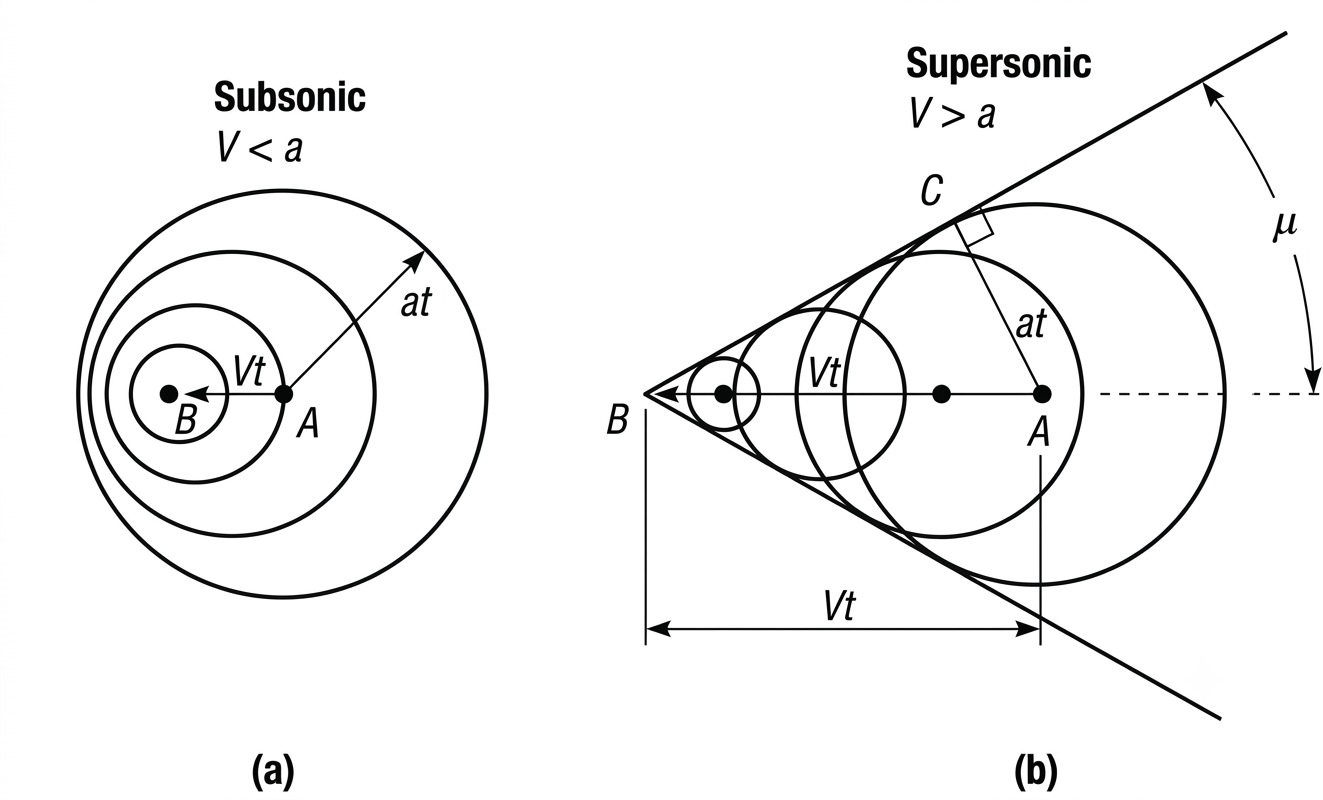
\includegraphics[width=0.5\textwidth]{figures/Moving sound waves.png}
    \caption{Propagation of information by an object moving at (a) subsonic speeds and (b) supersonic speeds, credit to Anderson \cite{TheBookOfAnderson}}
    \label{fig: Moving sound wave}
\end{figure}

Figure \ref{fig: Moving sound wave} shows an object leaving point A at a speed faster than the speed of sound, after a time interval $t$ it has traveled $Vt$, while the first emitted wave has only propagated a distance $at$. A supersonic wave is created tangentially to the emitted sound waves and has an oblique angle $\mu$ called the Mach Angle. The picture allows us to make the following geometric relationship:
\begin{equation}
    \sin \mu = \frac{a t}{V t} = \frac{1}{M}
\quad \Leftrightarrow \quad
\mu = \arcsin\!\left(\frac{1}{M}\right)
\end{equation}

\par The coalescence of the emitted waves creates an extremely thin region (of around $10^{-7}$m of magnitude) where the flow properties change drastically, in an almost explosive compression process that originates a seemingly discontinuous pressure increase across it \cite{TheBookOfAnderson}. When the emitted sound from the object becomes stronger, an oblique shock wave with an angle $\beta$ from the freestream air is formed, where $\beta > \mu$. Through this oblique shock wave, the pressure, density, temperature and entropy of the flow increases, while the total pressure, Mach number and velocity decreases. These relationships are described by the continuity, momentum and energy equations for oblique shocks, summarized by Equation \ref{equation: oblique continuity}, \ref{equation: oblique momentum} and \ref{equation: oblique energy} respectively, given the geometry of Figure \ref{fig: Oblique shock geometry}.

\begin{figure}[htbp]
    \centering
    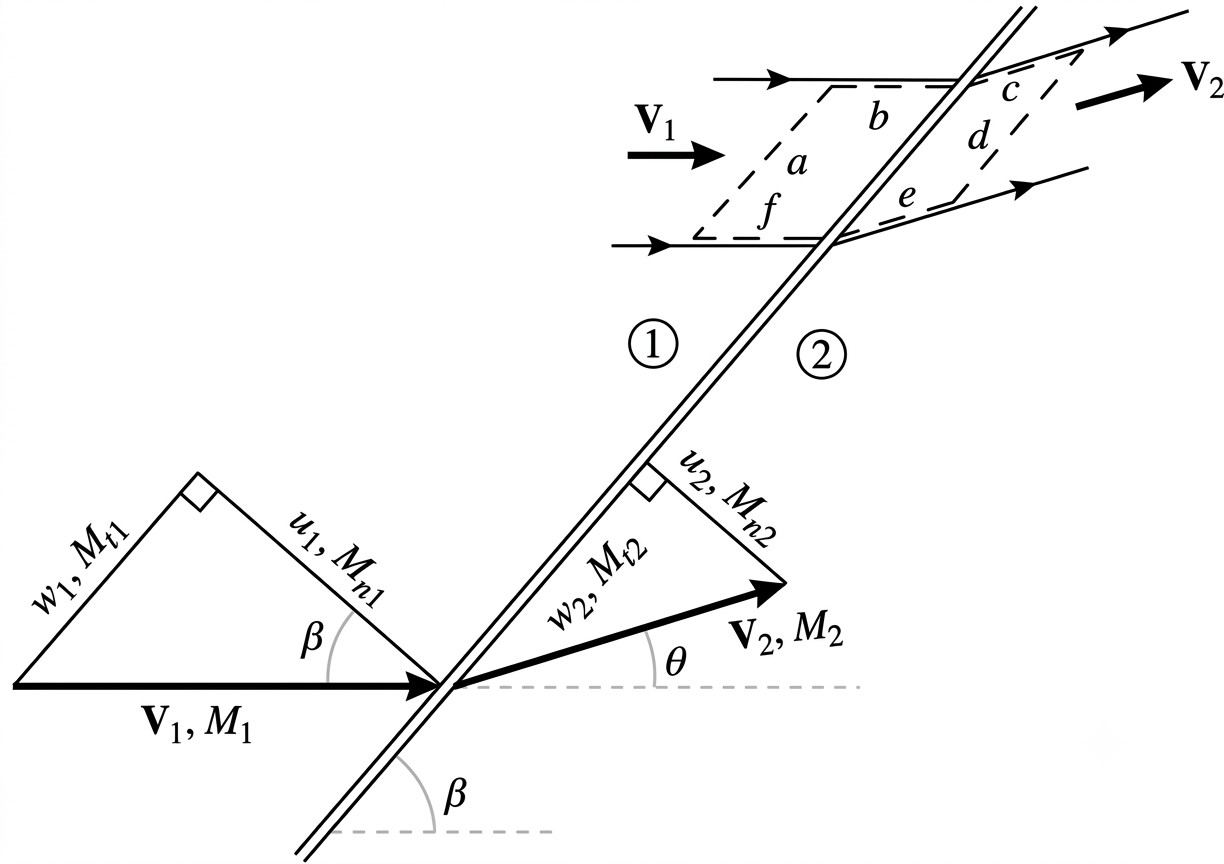
\includegraphics[width=0.5\textwidth]{figures/Oblique shock geometry.png}
    \caption{Oblique shock geometry, credit to Anderson \cite{TheBookOfAnderson}}
    \label{fig: Oblique shock geometry}
\end{figure}

\begin{align}
\rho_1u_1 &= \rho_2u_2 \label{equation: oblique continuity} \\
p_1 + \rho_1 u_1^2 &= p_2 + \rho_2 u_2^2 \label{equation: oblique momentum} \\
h_1 + \frac{u_1^2}{2} &= h_2 + \frac{u_2^2}{2} \label{equation: oblique energy}
\end{align}

\par These equations relate the flow properties before and after the shock. It is important to note that these changes depend only on the velocity component normal to the shock, with the tangential component maintaining constant. Considering a calorically perfect gas and adiabatic flow across the shock, it is possible to obtain the following relationships for $M_2, \rho_2$ and $p_2$ that rely only on $M_1$ and $\beta$.

\begin{align}
M_{n,1} &= M_1 \sin\beta, \\
 M_{n,2} &= M_2\sin(\beta-\theta)\\ 
M_{n,2}^{2}
&=
\frac{1 + M_{n,1}^{2}(\gamma - 1)/2}
{\gamma M_{n,1}^{2} - (\gamma - 1)/2}, \\
\frac{\rho_2}{\rho_1}
&=
\frac{(\gamma + 1)M_{n,1}^{2}}
{2 + (\gamma - 1)M_{n,1}^{2}}, \\
\frac{p_2}{p_1}
&=
1 + \left(\frac{2\gamma}{\gamma + 1}\right)
\left(M_{n,1}^{2} - 1\right).
\end{align}

\par These are important equations, as they allow the computation of the conditions after the shock by only knowing the initial flow conditions. Another important relationship defines the flow direction $\theta$ after it has passed through the oblique shock, called the $\theta-\beta-M$ relation. This equation gives two solutions for flows over concave wedges, defining a weak shock and strong shock pairing of $M_1$ and $\beta$. The classification of a shock as strong or weak relates to the pressure drop across it, the bigger the total pressure drop, the stronger the shock. Consequently, the bigger the density gradient as well. This relationship is shown below, together with equation 2.9 it shows how strong density gradients naturally appear in supersonic flow across shock waves.

\begin{equation}
\label{equation:theta-beta-M}
    \tan \theta = 2 \cot \beta \frac{M_1^2\sin^2\beta -1}{M_1^2(\gamma +\cos 2\beta )+2}
\end{equation}

Up until now only compressive waves have been discussed, however, a supersonic flow can also expand through a Prandtl-Meyer expansion fan. When a supersonic flow finds a convex corner instead of a concave one, it turns away from itself, creating a continuous low pressure zone that accelerates it even further. An important parameter in these scenarios is the Prandtl-Meyer Angle $\nu$, which can be used to know how much the flow must bend in order to achieve a certain Mach number $M_2$. Equation \ref{equation: Prandtl-Meyer function} and \ref{equation: Prandtl-Meyer turning angle} summarizes how $\nu$ can be used to find the convex corner angle and subsequent flow direction $\theta$.

\begin{equation}
\label{equation: Prandtl-Meyer function}
    \nu(M) = \sqrt{\frac{\gamma + 1}{\gamma - 1}} \tan^{-1} \sqrt{\frac{\gamma - 1}{\gamma + 1}\left(M^2 - 1\right)} - \tan^{-1} \sqrt{M^2 - 1}
\end{equation}

\begin{equation}
\label{equation: Prandtl-Meyer turning angle}
    \theta = \nu(M_2) - \nu(M_1)
\end{equation}

The flow through an expansion fan is isentropic, which means that entropy is conserved in the process. No change in entropy means that no losses are present, consequently total quantities such as temperature and pressure are also maintained. Through the isentropic relationships in Equations \ref{equation: isentropic pressure} and \ref{equation: isentropic density}, the static density and pressure after an expansion fan can be calculated. The equations shows that an increase in the Mach number leads to a decrease in both static density as well as pressure.

\begin{equation}
\label{equation: isentropic pressure}
    \frac{p_0}{p} = \left(1 + \frac{\gamma - 1}{2}M^2\right)^{\frac{\gamma}{\gamma - 1}}
\end{equation}

\begin{equation}
\label{equation: isentropic density}
    \frac{\rho_0}{\rho} = \left(1 + \frac{\gamma - 1}{2}M^2\right)^{\frac{1}{\gamma - 1}}
\end{equation}


\par This section clarifies the connection between compressible flow and density changes, by explaining how high-speeds generate compression and expansion waves that vary the flow's properties. The theory presented here can be used to interpret two notable study cases, the flow of a free high-speed jet and the flow structure of an aerospike nozzle exhaust. Since these variations in density produce corresponding variations in refractive index, shock and expansion structures can be detected using the deflection of light passing through the medium by employing schlieren methods. These techniques allow the visualization and quantification of the resulting density gradients, enabling experimental measurements to be compared with theoretical predictions.

\section{Compressible Jets}
\label{section: Compressible Jet Theory}

\par One important study case of compressible aerodynamics is the flow structure of a high pressure jet. Jets are produced by a flow coming from high pressure reservoir that passes through a nozzle outlet and meets a lower pressure environment. When the pressure between the nozzle inlet and the ambient air surpasses a certain threshold, the critical pressure ratio $NPR_c$, the Mach number at the minimum cross-section of the nozzle becomes 1 and the mass flow through the nozzle hits its maximum. The pressure ratio can continue to increase but the throat Mach number and mass flow will remain the same for that given geometry, this condition is called choked flow. If the geometry of the nozzle after the throat diverges, the flow expands, a favorable pressure gradient is established and the flow accelerates, increasing the Mach number. Depending on the pressure at the exit of the nozzle, a jet can be said: under-expanded, if $p_e > p_a$; perfectly expanded, if $p_e = p_a$ or over-expanded, if $p_e < p_a$. Figure \ref{fig: jet expansion regimes} shows the visual difference between these different cases. This section will focus on the flow structure of an under-expanded jet as it will be used later as a study case of the experimental campaign.

\begin{figure}[htbp]
    \centering
    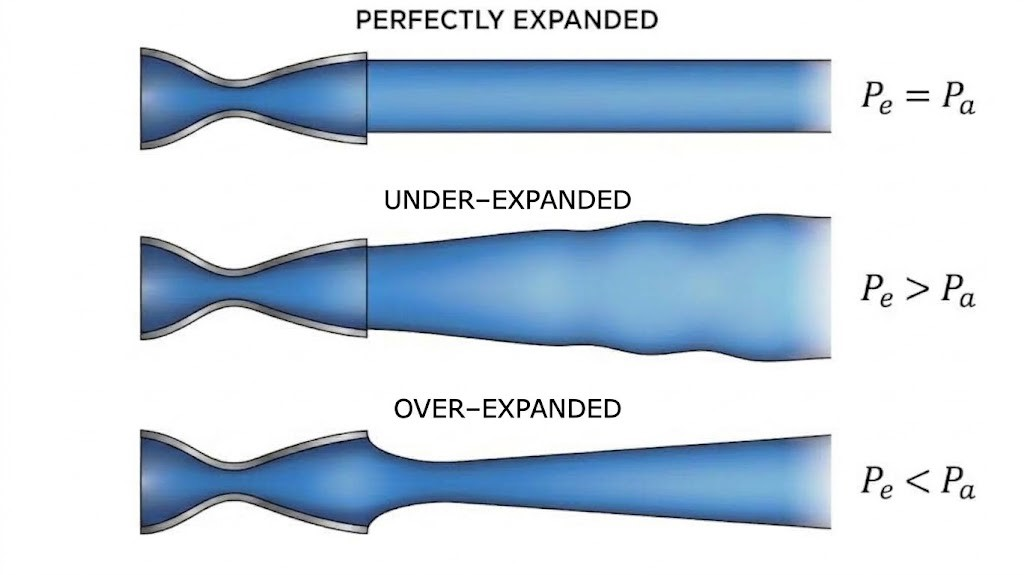
\includegraphics[width=0.8\textwidth]{figures/Under over and perfect expanded jets.jpg}
    \caption{Nozzle exit flow for the three expansion conditions: perfectly expanded ($p_e = p_a$), under-expanded ($p_e > p_a$) and over-expanded ($p_e < p_a$)}
    \label{fig: jet expansion regimes}
\end{figure}

\par Figure \ref{fig: planar underexpanded jet} shows the analytical solution of a planar under-expanded jet. It shows that the jet is marked by periodic structures called shock cells. These cells form as a mechanism of pressure adaptation between the nozzle exit and the ambient air through alternating Prandtl-Meyer expansion and compression waves \cite{vanHinsberg2014}. Since the the pressure at the nozzle exit is greater than the ambient pressure, the flow needs to expand to match the outside pressure. The results is a Prandtl-Meyer expansion fan anchored at the lip of the nozzle. These expansion waves are reflected at the axis of symmetry into another expansion fan, which in turn reflect at the jet boundary into compression waves. These converge into one another and coalesce, forming a shock. This shock increases the pressure, leading to another round of expansion waves. This process continues until, due to friction, the jet pressure equals the atmospheric pressure.


\begin{figure}[htbp]
    \centering
    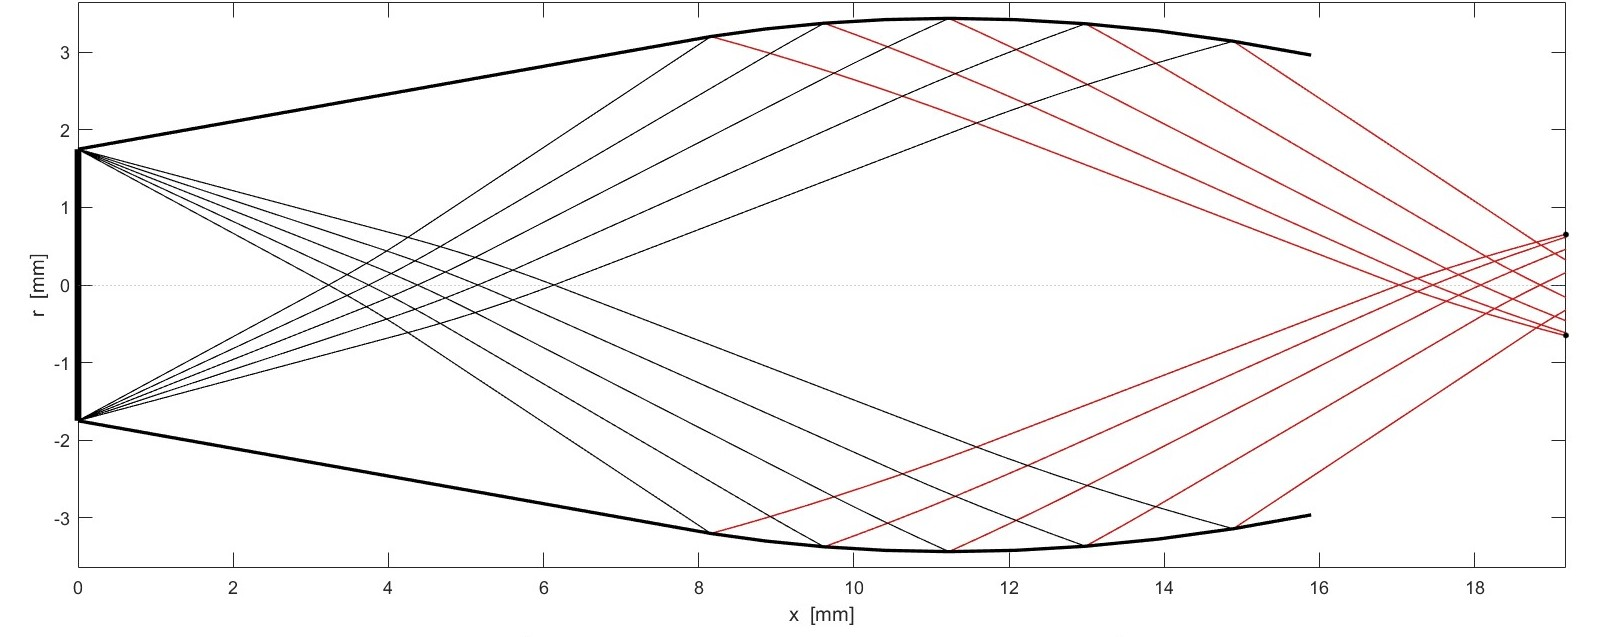
\includegraphics[width=\textwidth]{figures/under-expanded planar jet.jpg}
    \caption{Analytical solution of a planar under-expanded jet obtained using the Method of Characteristics with $M_e = 2$ and $p_e = 2 \cdot p_\infty$. The expansion waves leaving the nozzle lips (black) cross at the axis of symmetry, reflect at the jet boundary and return as compression waves (red), which converge and coalesce into a shock in the black dots at x= $19$mm}
    \label{fig: planar underexpanded jet}
\end{figure}

The three Figures \ref{fig: moderately underexpanded jet}, \ref{fig: highly underexpanded jet} and \ref{fig: unique barrel underexpanded jet} show sketches of under-expanded circular jets at different NPRs \cite{Duronio2023}. Due to it's axissymetry, the circular jet has a different structure to the planar case, displaying an early formation of an oblique shock extending from the lip to the jet axis, often called \emph{Intercepting shock}. When the NPR is between 2 and 4, as in Figure \ref{fig: moderately underexpanded jet}, this oblique shock reflects at the jet axis and goes to the shear layer, where it turns into an expansion fan, thus forming an "X" shape at each shock cell. For higher NPRs between 4 and 7, Figure \ref{fig: highly underexpanded jet}, the intercepting shock transitions to a singular reflection and produces a normal shock called \emph{Mach disk}, which gives each shock cell a "barrel" shape. For even higher NPRs, Figure \ref{fig: unique barrel underexpanded jet}, the jet is dominated by a single barrel. The last case is marked by a decreased jet boundary diameter and a very long plume caused by entraining air.

\begin{figure}[htbp]
    \centering
    \begin{subfigure}[b]{0.32\textwidth}
        \centering
        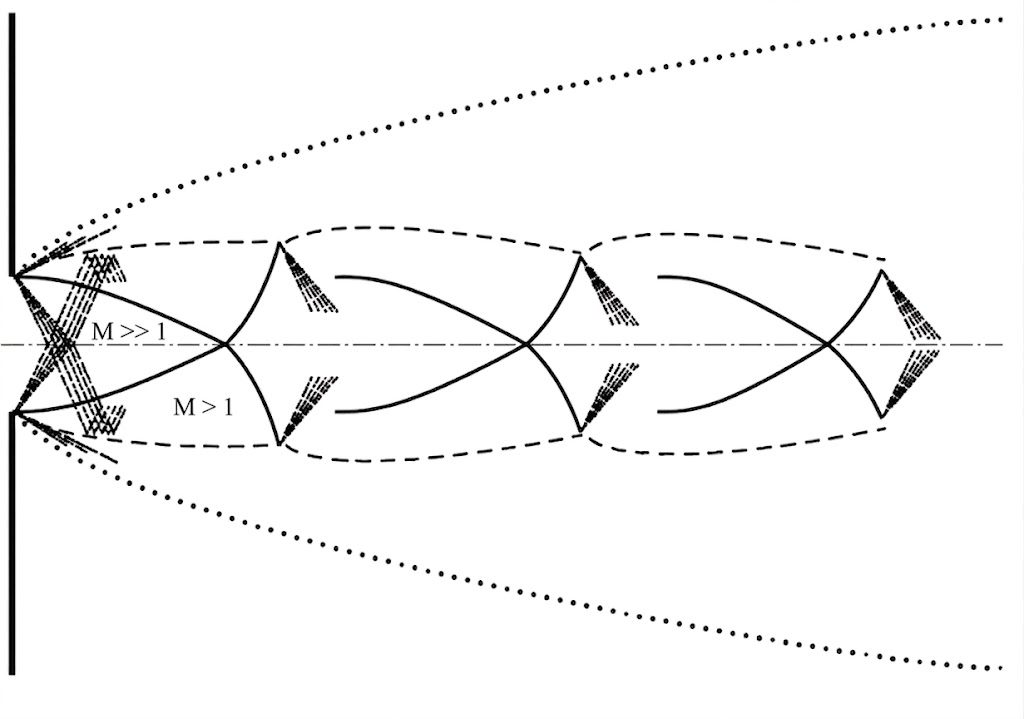
\includegraphics[width=\textwidth]{figures/moderately under-expanded jet.jpg}
        \caption{Moderately under-expanded, $2 < NPR < 4$}
        \label{fig: moderately underexpanded jet}
    \end{subfigure}
    \hfill
    \begin{subfigure}[b]{0.32\textwidth}
        \centering
        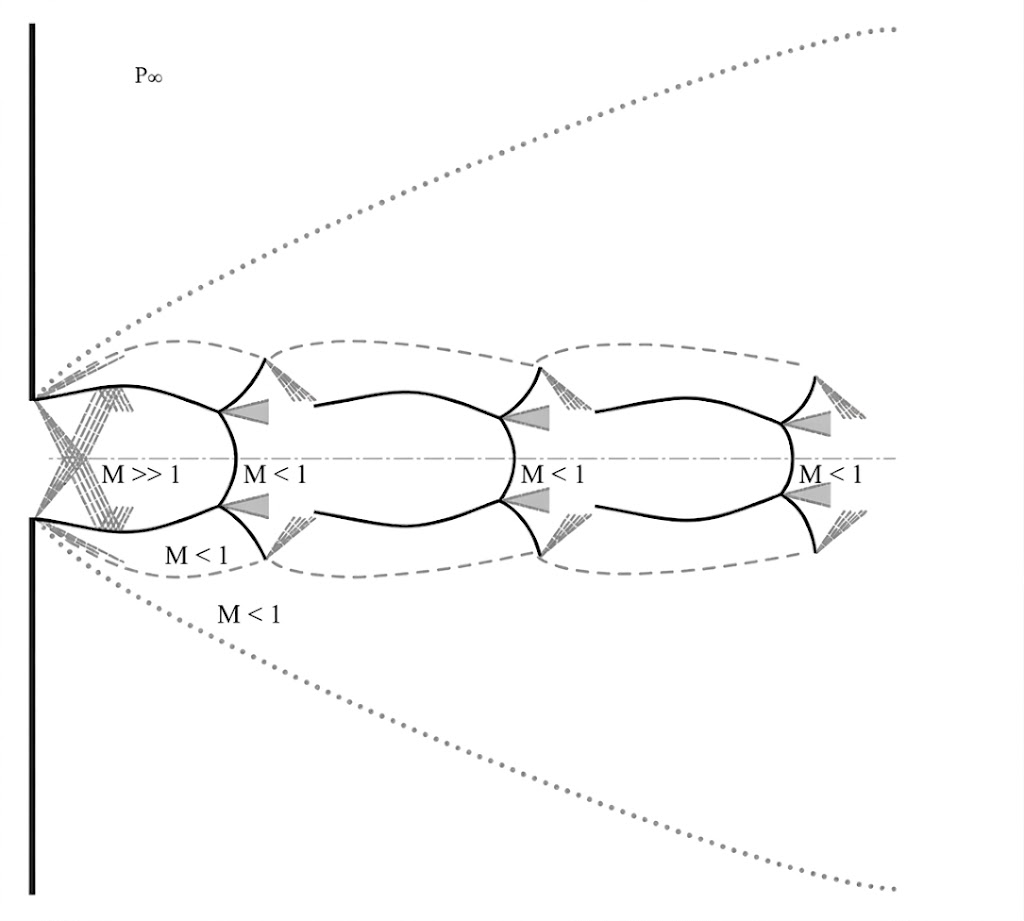
\includegraphics[width=\textwidth]{figures/highly under-expanded jet.jpg}
        \caption{Highly under-expanded, $4 < NPR < 7$}
        \label{fig: highly underexpanded jet}
    \end{subfigure}
    \hfill
    \begin{subfigure}[b]{0.32\textwidth}
        \centering
        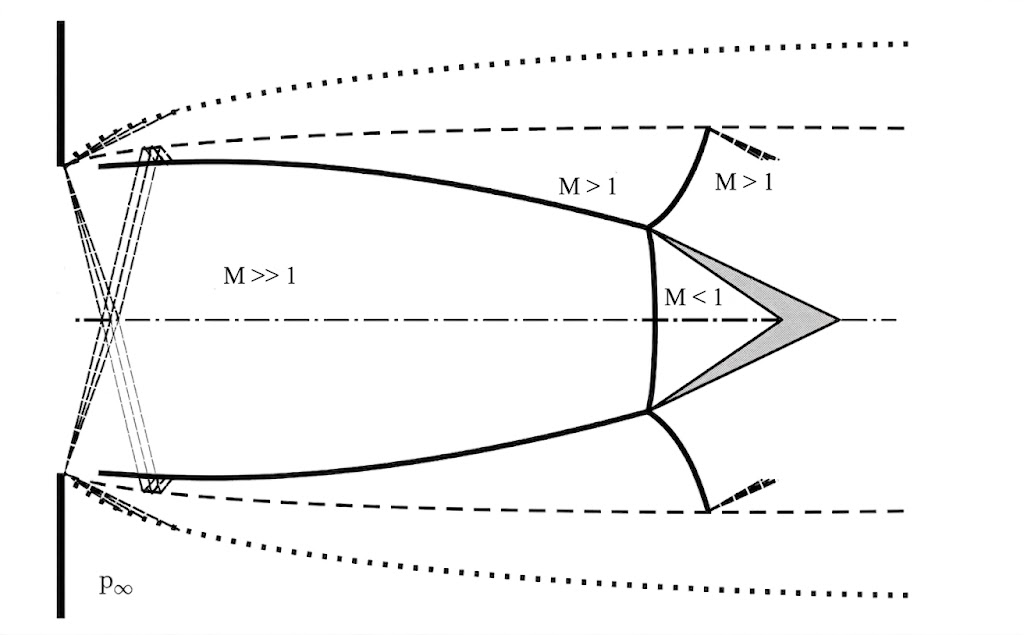
\includegraphics[width=\textwidth]{figures/unique barrel under-expanded jet.jpg}
        \caption{Single Barrel Structure, $NPR > 7$}
        \label{fig: unique barrel underexpanded jet}
    \end{subfigure}
    \caption{Sketches of circular under-expanded jets at increasing nozzle pressure ratio, credit to Duronio et al. \cite{Duronio2023}}
    \label{fig: circular underexpanded jets}
\end{figure}

As hinted by the scale of the sketches in Figure \ref{fig: circular underexpanded jets}, the $NPR$  also changes the length of the shock cells, $L_s$. Robert Emden was the first to correlate a weighted average of the $L_s$ of under-expanded choked jets with the $NPR$ in 1899 \cite{Powell2010, Emden1899}. After a series of experiments he reached the format of equation \ref{equation: Emden Formula}, where $k$ is a numerical coefficient that varies with the nozzle geometry and NPR range. The value of $k$ changed from 0.77 to 1.02 during the campaign, so Emden averaged the results of different nozzles to obtain $k = 0.88$. Later, Hartmann \& Lazarus \cite{Hartmann1941} used Emden's format with the average of all the cells except the first, achieving $k = 1.07$. They also correlated only the first shock cell length and introduced a constant term independent of $NPR$, obtaining the format of equation \ref{equation: Lazarus-Hartmann Formula}, with $a = 0.98$ and $b = 0.3$.
\begin{equation}
    \label{equation: Emden Formula}
    \frac{L_s}{d_N} = k\sqrt{NPR - NPR_c}
\end{equation}

\begin{equation}
    \label{equation: Lazarus-Hartmann Formula}
    \frac{L_s}{d_N} = a\sqrt{NPR - NPR_c}+b
\end{equation}

A circular jet created by a choked duct will be used to attest the capabilities of SBOS in producing a quantitative density field. In that context, this knowledge on axissymetric jet structure will be important to visually interpret the results after the experimental campaign. Furthermore, similar structures to those explained here for are present in different other applications, such as an aerospike nozzle. The next subsection will give a brief summary of the flow through a linear arospike nozzle and use much of what has been said here for that purpose.

\section{Aerospike Nozzle Flow}
\label{section: aerospike nozzle theory}
The distinct feature of an aerospike nozzle is the presence of its ramp right after its  exhaust. The ramp is designed so that the expansion fan anchored at the outside lip is not disturbed by the reflection of its own waves \cite{Wisse2005}. In the design condition, the flow expands through these waves, accelerating and reducing its static pressure, until design conditions are met, $M_{design}$ and $(p/p_a)_{design}$. In under-expanded condition, the same pressure adaptation process that happened in the free under-expanded jet now occurs in the ramp, where the flow is redirected to be parallel to the centerline. The result is a passive pressure adaptation mechanism that allows an aerospike to keep its thrust efficiency for a wide range of ambient pressures. In over-expanded condition, the flow is expanded below ambient pressure, the maximum turning angle of the fan increases, redirecting part of the exhaust flow sideways. Also, a shock may appear downstream so that ambient pressure is reached. Both mechanisms lead to a loss in thrust efficiency, so engineers try to avoid this condition and favor under-expanded and perfectly expanded flow. Figure \ref{fig: aerospike expansion regimes} shows the flow structure of an aerospike in under, perfectly and over expanded conditions.

\begin{figure}[htbp]
    \centering
    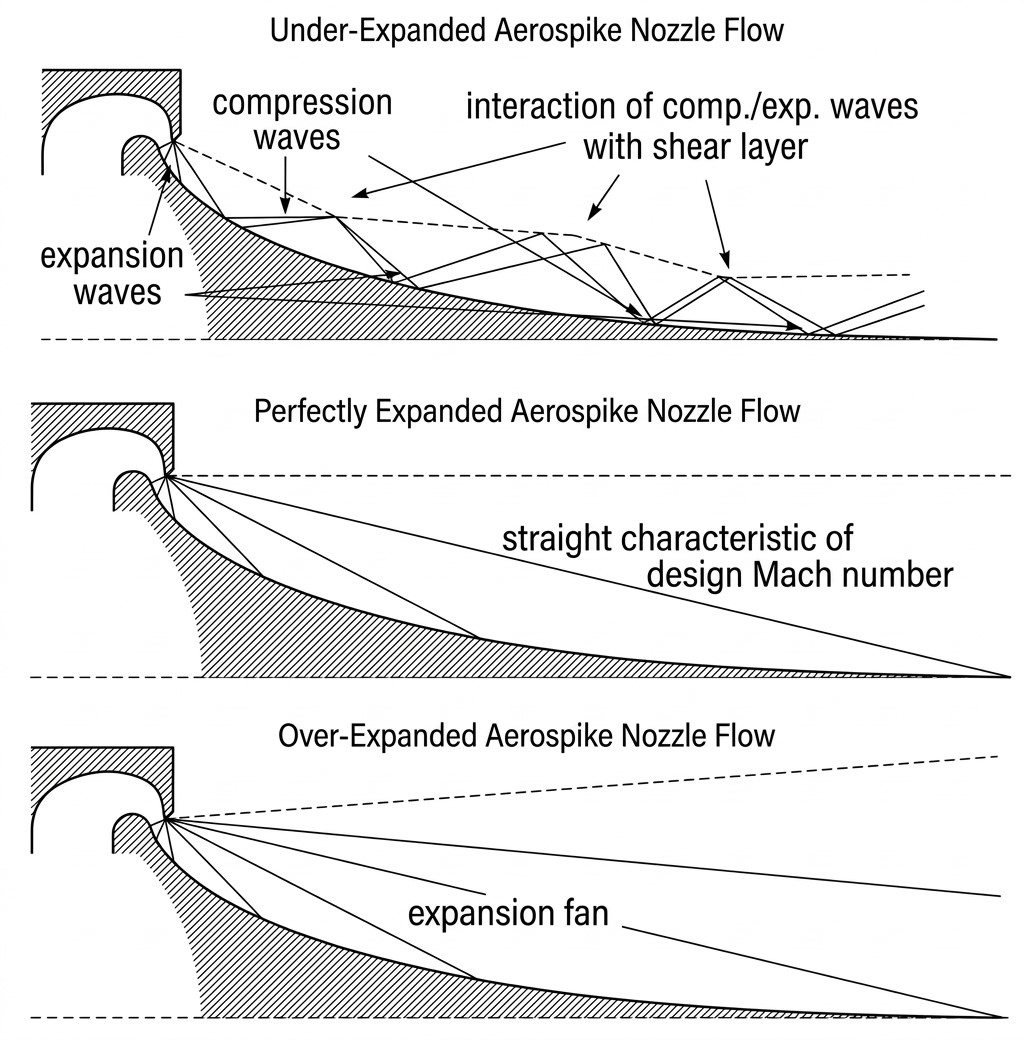
\includegraphics[width=0.6\textwidth]{figures/under perfect and over expanded aerospike.jpg}
    \caption{Flow structure of a linear aerospike nozzle in under-expanded, perfectly expanded and over-expanded conditions, credit to Wisse \cite{Wisse2005}}
    \label{fig: aerospike expansion regimes}
\end{figure}

It's the pressure adaptation feature present in an aerospike at under-expanded condition that makes it interesting for Single Stage to Orbit (SSTO) vehicles \cite{Wisse2005}. As shown in Figure \ref{fig: aerospike expansion regimes}, the process resembles the succession of expansion and compression waves present in the free under-expanded jet of Figure \ref{fig: planar underexpanded jet}. The mechanism always begins with an expansion wave at the outside lip of the exhaust exit. These waves reach the ramp and due to its concave geometry, the flow is compressed and reflect as compression waves. In the shear layer, the compression waves reflect into waves of other type and are redirected to the ramp. At this stage however, the curvature of the ramp is less accentuated and the waves reflect at the ramp to ones of the same family. The process continues with waves changing its type at the jet boundary and maintaining it when hitting the ramp, gradually fluctuating the ramp pressure around ambient conditions. This way, the flow is directed to be parallel to the centerline and there are no abrupt pressure differences capable of producing strong loss inducing shocks.

%The flow through the ramp of an aerospike nozzle will be investigated later using SBOS as a demonstration of the imaging method capabilities

The flow through the ramp of an aerospike nozzle will be investigated later using SBOS  to assess if the method has sufficient resolution and sensitivity to correctly study such complex flow field . In that context, the description of the flow physics will be of utmost important to assess if the method has sufficient resolution and sensitivity to correctly study the application. It is now clear from the previous sections how high-speeds and geometry leads to different flow structures that vary the fluid's density. The next section will explain how density influences the bending of light moving through a fluid, which is the fundamental principle behind optical density measurement techniques.

\section{Refraction}
\label{section: Refraction}
\par Refraction is the change in direction of a light ray as it propagates through a medium with spatially varying refractive index. This index is the ratio between the speed of light through vacuum, $c_0 \approx 3 \cdot 10^8$ m/s, and the speed of light through the medium, $c: n=c_0/c$.

\par The refractive index is a function of the light’s wavelength $\lambda$, and the thermochemical state of the environment it passes through. If $n$ is known at a certain wavelength and thermochemical state, it can be extrapolated to other states through the Lorentz-Lorentz equation, where $A$ is the molar refractivity, dependent on the wavelength, and $W_M$ the mean molecular weight \cite{Schmidt2025}.

\begin{equation}
    \frac{n^2 - 1}{\rho \left(n^2 + 2\right)}
=
\frac{A}{W_M}
=
\text{constant}
\end{equation}

\par The Gladstone-Dale is the linearization of this relationship for gases, where $n$ is almost 1 \cite{Head2021}. 

\begin{equation}
    n = 1 + G \rho
\end{equation}

\par This relationship directly links density with the refractive index, which in turn can be given by the distortion of light through the medium. $G$ is the Gladstone-Dale coefficient \cite{Head2021} \cite{Settles2001}.

\par As shown in Figure \ref{fig: Diagrams of light refraction}, when light passes from one medium to another it can behave differently depending on the refractive index field of the subsequent medium. The light’s interaction between two homogeneous media, shown in Figure \ref{fig: Diagrams of light refraction}a, is given by Snell’s Law of Refraction.

\begin{equation}
    n_1 \sin{\varepsilon_1} = n_2 \sin{\varepsilon_2}
\end{equation}

\begin{figure}[htbp]
    \centering
    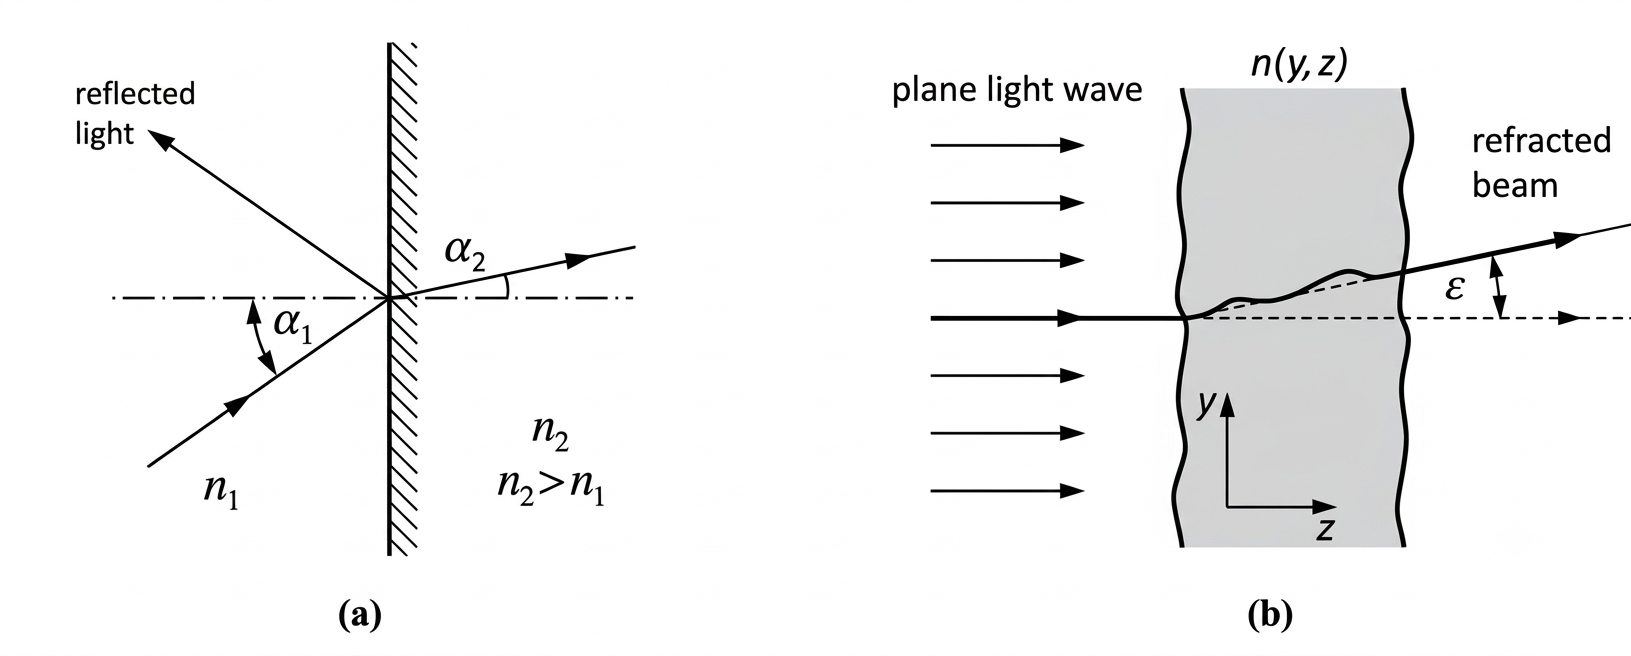
\includegraphics[width=0.8\textwidth]{figures/Diagrams of light refraction.png}
    \caption{Diagrams of Light refraction: (a) Change in the beam's direction between two homogeneous media as described by Snell's Law and (b) light refraction through an irregularly distributed refractive index environment. Credit to Schmidt et al. \cite{Schmidt2025}}
    \label{fig: Diagrams of light refraction}
\end{figure}

\par However, for inhomogeneous environments, as in Figure \ref{fig: Diagrams of light refraction}b, the change in light’s direction is not discrete. So a generalization must be performed to relate the deflection $\varepsilon$ to the refractive index field. Assuming small angle deflection and small refractive index gradient, the equation below is obtained, with $z$ being the line-of-sight direction \cite{Settles2001}.

\begin{equation}
    d\varepsilon_x = \frac{1}{n_o}\frac{\partial n}{\partial x}\,dz
\end{equation}

\par The total deflection is the integral of $d\varepsilon$ along the ray path, as is shown below. An analogous equation exists for $y$, by substituting it in $x$.

\begin{equation}
\label{equation: displacement integral}
    \varepsilon_x
=
\frac{1}{n_o}
\int \frac{\partial n}{\partial x} dz
\end{equation}

\par Now, if a substitution is applied with the Gladstone-Dale relationship, one can obtain:

\begin{equation}
\label{equation:epsilon-nabla rho}
    \vec{\varepsilon}
=
\frac{G}{n_o}
\int \nabla \rho \, dz
\end{equation}

\par Equation \ref{equation:epsilon-nabla rho} links directly the light deviation vector to the density gradient through media. Thus, in order to obtain a quantitative measure of the density field through a test section, one could employ a method to measure the displacement of light after passing through it. If the transversal refractive gradients are independent to the line of sight direction, such as a 2D planar flow, Equation \ref{equation:epsilon-nabla rho} can be simplified into Equation \ref{equation: Displacement and Density Gradient} for $x$, where $W$ is the refractive object thickness \cite{RajendranDotTracking}.

\begin{equation}
    \label{equation: Displacement and Density Gradient}
    \varepsilon_x = \frac{G\cdot W}{n_0} \frac{\partial \rho}{\partial x}
\end{equation}

The equation shows that light bends in the direction of the desnity gradient, that is, the direction of highest density. For a 2D planar flow, if the displacements caused by light passing through it are measured in a plane, the object density gradient can be computed and integrated to obtain a density field. For a more complex 3D flow, multiple line of-sights must be used to reconstruct a tomographic image of the density. However, some 3D flows can be reconstructed with only a 2D view due to it's symmetry. An axissymetric body is one of such case which occur frequently in various applications. The next section will demonstrate how axissymetry can be used to obtain the 3D density field using 2D displacement vectors.

\subsection{Axisymmetric Refractive Field}
\label{subsection: Axisymmetric Refractive Field}

When a refractive object is axially symmetric, it is possible to reconstruct its whole density distribution with only a 2D snapshot of the light displacements through it. In such scenario, the image is a 2D projection of a 3D axisymmetric body, and the inverse Abel transform can be used to obtain its radial and axial profile \cite{Abel1826}. Consider the case in Figure \ref{fig: Abel transform} and Equation \ref{equation: displacement integral} for y, it can be integrated in y in both sides into Equation \ref{equation: integral of epsilon}, which removes the partial derivative through the fundamental theorem of calculus.

\begin{figure}[h]
    \centering
    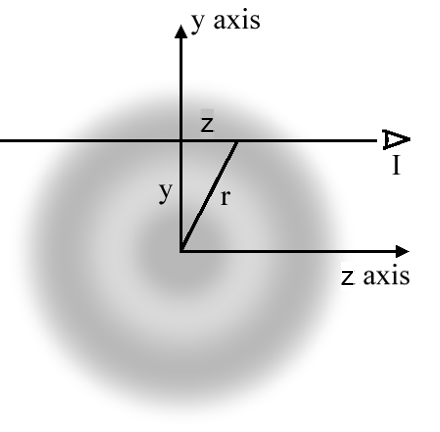
\includegraphics[width=0.3\textwidth]{figures/AbelTransform.png}
    \caption{Diagram of the geometry of an axisymmetric body being seen by an observer in I. If the body, in grey, is described by a function $f(r)$, the observer will see its projection $F(y)$, which is its Abel transform}
    \label{fig: Abel transform}
\end{figure}

\begin{equation}
\label{equation: integral of epsilon }
    E_y = \frac{2}{n_0}\int_0^R [n(r) - n_0]dz
\end{equation}

Now, by changing $z$ for the radius $r$, $E_y$ becomes the plain Abel transform of the refractive index $n$ in Equation \ref{equation: Abel transform of n}. This means that when the inverse Abel transformation is applied to $E_y$, a radial profile of $n$ is obtained, which can be translated to the density through the Gladstone-Dale relation.

\begin{equation}
    \label{equation: Abel transform of n}
    E_y = \frac{2}{n_0} \int_0^R \frac{[n(r) - n_0]}{\sqrt{r^2-y^2}}r dr
\end{equation}

This chapter has shown how changes in density can emerge in different flow conditions and how these variations modify the flow's refractive properties. It is the ability to relate optical distortions to density gradients that forms the foundation of schlieren-based diagnostic techniques. The next chapter will treat these methods by presenting a brief history of how researchers have been able to measure the bending of light and translate it into qualitative and quantitative thermodynamic measures over the years, culminating in the state of the art and the topic of this thesis, SBOS.
\chapter{Optical Density Measurement Techniques}
\label{chapter: LiteratureReview}

\par Several techniques have been developed which use light refraction as a principle to visualize changes in density. These methods can be grouped into classical techniques such as Shadowgraphy, Schlieren, Interferometry and modern methods, such as Background Oriented Schlieren and its variants. This section will provide a brief historical background on classical density gradient measurement techniques and explain how these methods have developed leading up to BOS. Then, a more detailed literature review is given in BOS and SBOS to better define the state of the art of these methods and provide context to the research gap that this thesis aims to fulfill.

%detailed description of the schlieren-based methods is given, finishing with laser %speckled BOS and the research gap.

\section{Classical Methods}

\par The earliest report of a density gradient measurement technique dates back to the 1600s, when Hooke tried to visualize the flow around a candle flame with the aid of a lens \cite{Settles2001}. His experiments resemble setups used for Shadowgraphy, where a test subject is positioned in between an observer and a light source, as shown in 
Figure \ref{fig: Hooke shadowgraphy}. The variations in the refractive index at the test section bends the light coming from the source, producing shadows and brighter regions captured by the observer. Shadowgraphy is valued by its simplicity, however it provides only qualitative results, as quantitative reconstruction is difficult due to second-derivative sensitivity on the line-of-sight integration. Nevertheless, Shadowgraphy continues to be an important flow visualization technique, complementing other more complex methods in the study of compressible flows \cite{Settles2017}.

\begin{figure}[htbp]
    \centering
    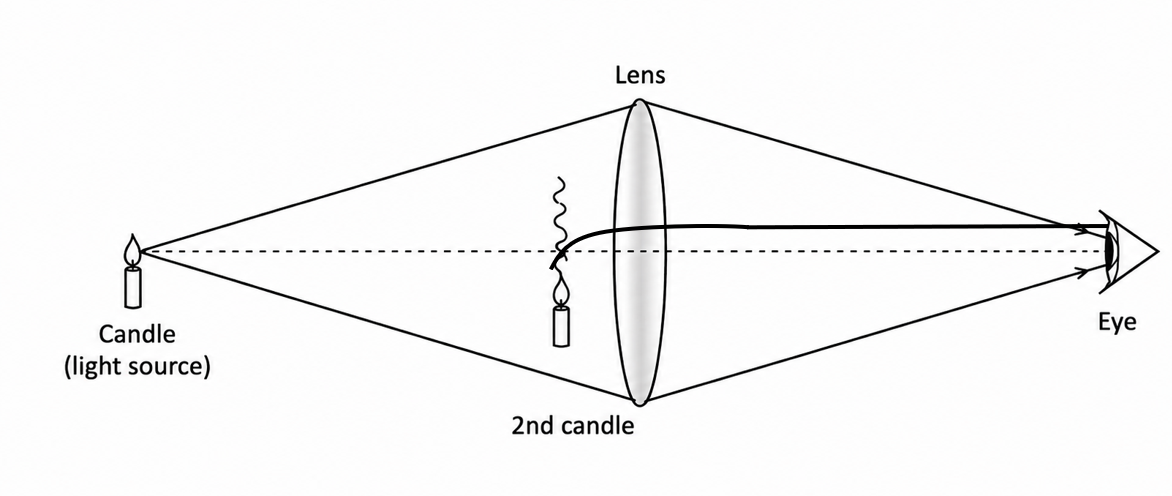
\includegraphics[width=0.8\textwidth]{figures/Hooke shadowgraphy setup.png}
    \caption{Hooke’s shadowgraphy setup, credit Settles \cite{Settles2001}}
    \label{fig: Hooke shadowgraphy}
\end{figure}

\par In the 19th century, Toepler coined the term “Schlieren” and was the first to apply the technique as a scientific tool \cite{Settles2001}. Toepler’s setup used a lens to focus the distorted light coming from the test section to a point where a knife’s edge was placed to block half of the image. The knife served as a filter and allowed Toepler to measure the light’s deviation on the axis perpendicular to it, quantifying the density gradient in that direction. A simple Schlieren setup can be seen in Figure \ref{fig: Schlieren setup}. The technique provides high sensitivity and has been extensively used throughout the years for the research of compressible flows, being famously implemented by Ernst Mach on the study of shock waves. However, the need for big, costly optical elements for larger scales and the sensitivity to only one axis put a constraint on the method, motivating the implementation of simpler whole-field techniques with a larger field of view. Nevertheless, the use of Schlieren is still relevant to this day and many derivations of the method exist, providing unique advantages and applications \cite{Settles2017}.

\begin{figure}[htbp]
    \centering
    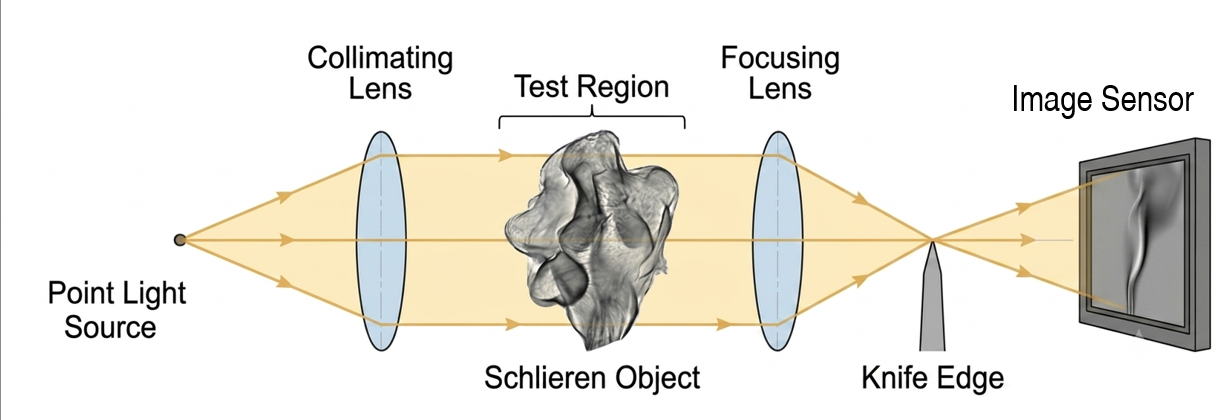
\includegraphics[trim={1cm 0cm 0cm 0cm}, clip, width=0.8\textwidth]{figures/Schlieren setup.png}
    \caption{Illustration of a simple schlieren setup}
    \label{fig: Schlieren setup}
\end{figure}


\par Another method that relies on light deviations to measure density gradients is interferometry. In this technique, the imaging sensor is exposed to two laser beams, one passes through the test subject, which bends it and slows it down; the other one reaches the sensor unaffected. When both beams interact with the imaging sensor, they interfere, producing interference fringes that can be related to the refractive index change in the test subject. One important application of the method is the use of laser speckle photography for interferometry by Debrus \cite{Debrus1972} and Köpf \cite{Kopf1972}. They used a ground glass lens diffuser to scatter the laser beam and produce a speckle pattern, then exposing a sensitive film to this laser-speckled pattern when there is an active flow and no flow passing through it. The double exposure produces Young’s fringes in the film which relates to light deviation \cite{NikitaFominBook}. Köpf’s setup can be seen in Figure \ref{fig: laser speckled interferometry}. This early use of speckle patterns foreshadows its later application in SBOS configurations.

\begin{figure}[htbp]
    \centering
    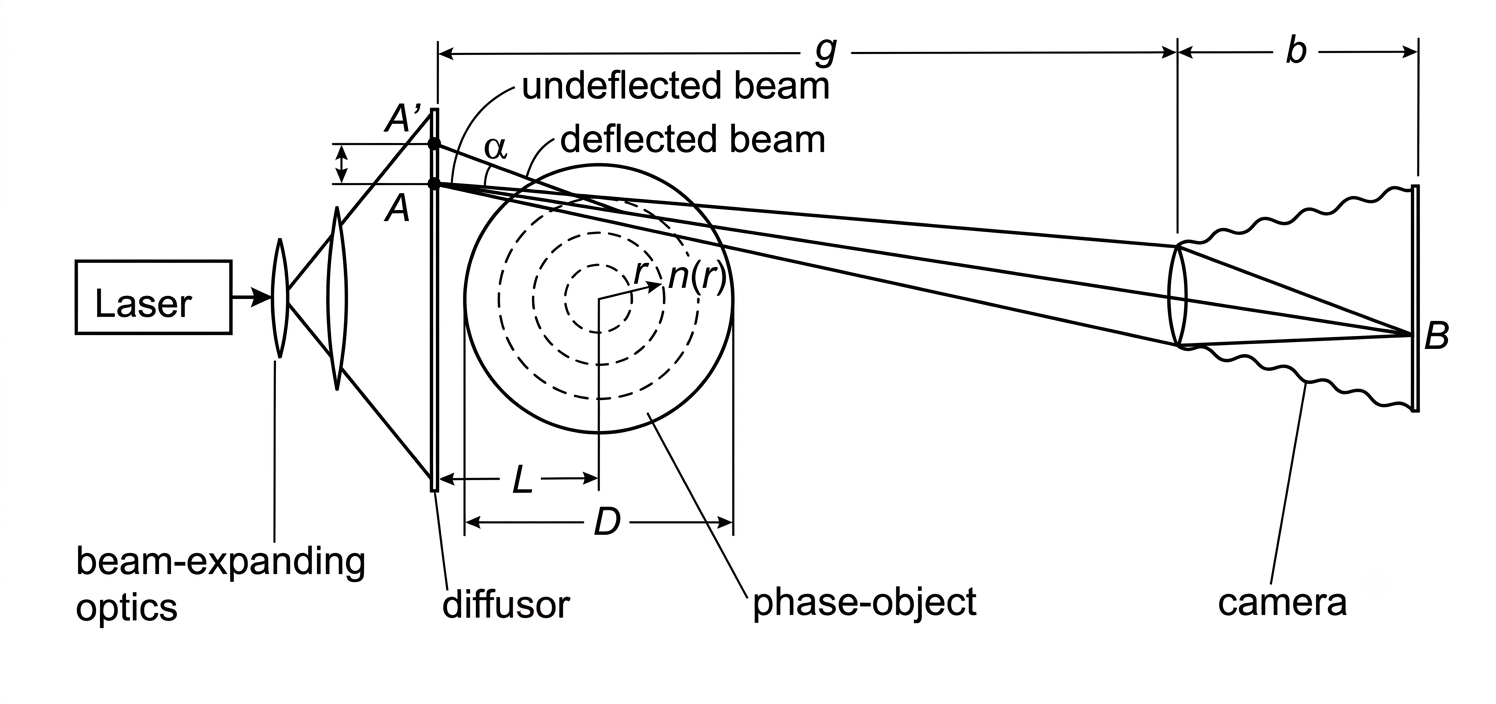
\includegraphics[width=0.8\textwidth]{figures/laser speckled interferometry.png}
    \caption{Laser-speckled Interferometry setup, credit to Köpf \cite{Kopf1972}}
    \label{fig: laser speckled interferometry}
\end{figure}

\par As aforementioned, the classical density gradient methods are still relevant to this day \cite{Settles2017}. Shadowgraphy’s simplicity gives relevant quick qualitative insights into the flow; Schlieren’s high sensitivity and small post-processing requirement motivates its use in many cases, with new developments even using colored filters to get information on more than one axis at a time; and Interferometry allowing for larger fields of view than the latter two. However, each of them lack in some way, as Shadowgraphy can only give qualitative results; Schlieren fails at larger scales and directional sensitivity; and interferometry uses a complicated setup with complex post-processing. Background Oriented Schlieren takes on the advantages of the latter methods and ameliorates its drawbacks, providing a simple, whole-field, scalable, high sensitivity technique, but still leaving some room for improvement, as will be discussed in the next section.

\section{Background Oriented Schlieren}
\label{section: Background Oriented Schlieren}
In the year 2000, a new technique emerged taking advantage of new sensors and image processing algorithms, the Background Oriented Schlieren (BOS) technique \cite{Raffel2001}. The method consists in measuring the distortion of a background image due to the presence of a test flow. To achieve that, a background pattern is positioned after the test section, an image of the pattern is captured when no flow is present and another when there is a density gradient that distorts the background. This displacement is quantified using image sensing algorithms and can be related to the flow’s density as shown in section \ref{section: Refraction} \cite{Schmidt2025}. This method greatly simplifies the Schlieren setup, provides a whole field analysis of the test section and it is easier to scale than the traditional methods. These advantages, together with its accuracy and non-intrusiveness, made the technique quite popular among experimentalists, with many improved versions being proposed over the years. Figure \ref{fig: BOS setup Raffel} shows a typical BOS setup.

\begin{figure}[htbp]
    \centering
    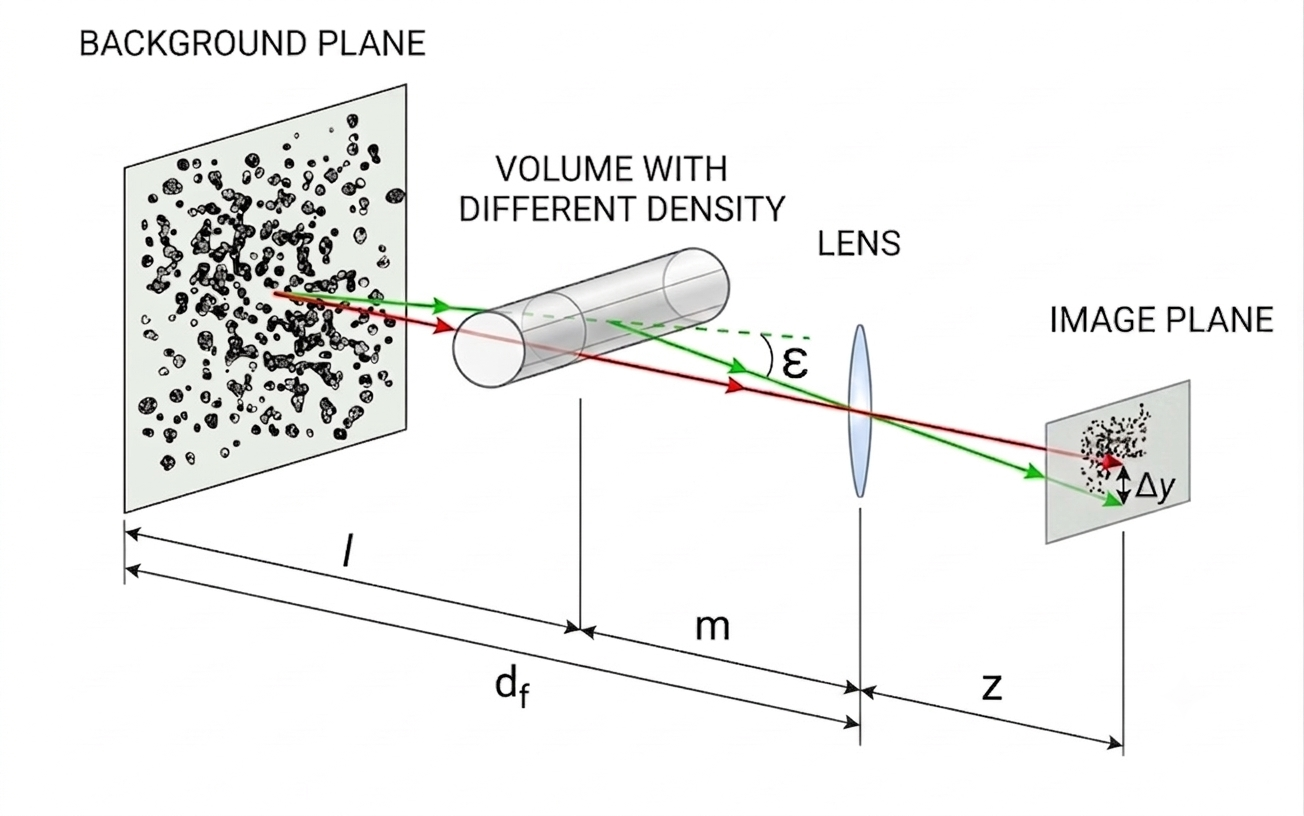
\includegraphics[width=0.6\textwidth]{figures/Raffel BOS setup.png}
    \caption{BOS setup, credit to Raffel \cite{Raffel2001}}
    \label{fig: BOS setup Raffel}
\end{figure}

%%% Now it comes the question. Should I talk about the equations now? Or leave then to mathodologies? a bit of both

\par Practical guidelines for the design of BOS setups have been established in the literature. Both Gojani et al. \cite{Gojani&Obayashi} and Schwarz et al.
\cite{Schwarz&Braukmann} highlighted the importance of sensitivity and spatial
resolution in defining the optical configuration for BOS. Sensitivity $S$ can be
interpreted as the capacity of the setup to magnify the light distortion from the
refractive object, and is set by the product of the defocus distance and the optical
magnification, $S = lM$. Spatial resolution refers to the smallest spatial scale of the studied flow that can be resolved, that is, the size of the smallest distinguishable flow feature $s_{min}$. It is governed by the blur of the refractive object, quantified by the circle of confusion $CoC$ \cite{Greenleaf1950}, its derivation can be found in Appendix \ref{Appendix: CoC derivation}. The complete set of relations linking these two performance parameters to the physical layout of the setup is assembled in Chapter \ref{chapter: methodology}, where it forms the basis of the design strategy of this thesis.

\par Sensitivity grows with the distance between the refractive object and the
background, so the first instinct is to place the background as far away as possible.
The returns diminish, however: as the defocus distance grows without bound the
sensitivity saturates at the focal length of the lens, $S \rightarrow f$. A longer
focal length therefore raises the ceiling on achievable sensitivity, but $f$ is itself
constrained by the desired field of view $L_{FoV_{obj}}$ and the camera sensor size
$L_{sens}$ \cite{Schmidt2025}. This asymptotic behavior is examined quantitatively in
Chapter \ref{chapter: methodology}.

\par Furthermore, there is an inherent focusing problem on BOS. During the setup assembly, one would like to focus on the background for better contrast and position the background farther away from the test subject for increased sensitivity. But, as the distance between the test subject and the in-focus plane increases, the blur of the refractive object is worsened and hinders the spatial resolution of the setup. One strategy would be to increase the depth of field, thus increasing the “thickness” of the in-focus plane, by increasing the $f_\#$ number (see Appendix~\ref{Appendix: CoC derivation} and \cite{Greenleaf1950}). However, reducing the lens aperture decreases the illumination reaching the camera sensor, which leads to reduced light signal and contrast. Consequently, a compromise must be made between spatial resolution and sensitivity, tuning the optical setup to achieve the maximum signal and acceptable blur.

\par Although it provides advantages compared to classical methods, the design of a BOS setup is marked by constraints and compromises. The achievable sensitivity is limited by the geometric configuration as increasing the sensitivity requires larger optical distances, which in turn degrade spatial resolution due to increased blur. Careful optimization of parameters is required to balance these competing effects. These limitations motivate the exploration of alternative approaches. By using Laser-Speckled Background Oriented Schlieren (SBOS) many of these shortcomings can be overcome, as it will be discussed. 

\par Before introducing SBOS, however, further aspects of BOS deserve attention. The first corresponds to an ambiguity found in the literature regarding the optical spatial resolution. Then, it will be discussed the influence of the imaging hardware and post-processing,as both bound accuracy and resolution as much as optics do. Lastly, a range of variants that has been derived from BOS over the past twenty-five years will be presented, which gives the context for understanding both the strengths and the particular niche SBOS occupies. The next subsections will treat these matters.
%I should maybe add a picture here

\subsection{Optical Spatial Resolution}
\label{subsection: Optical Spatial Resolution}
\par As  aforementioned, spatial resolution refers to the size of the smallest distinguishable feature in the image and in optical configurations that is limited by the amount of blur of the object. It is worth noting that, despite the clear conceptual definition, there is no consensus on a definitive mathematical formulation of this quantity in the literature, leading to ambiguity. Schwarz et al. \cite{Schwarz&Braukmann} tested various BOS setups and related the concept of Circle of Confusion ($CoC$) from Greenleaf \cite{Greenleaf1950} to the spatial resolution of the setup. Meanwhile, Gojani et al. \cite{Gojani&Obayashi} derived an equation for the spatial resolution using geometry and theoretical assumptions. The two formulations do not yield the same result, so an investigation on the methods used to obtain them was conducted.

\par Gojani et al.'s mathematical formulation has sound theoretical grounds, however it presents ambiguities and lack of experimental data to support some claims.  The paper makes the fundamental assumption that anything inside the $CoC$ is indistinguishable. Therefore, the smallest distinguishable size is obtained by tracing the cone of light from the $CoC$ in the sensor plane to a size in the object plane when the setup is focused on another plane (such as the background). Figure \ref{fig: Gojani cone of light} shows the cone of light used by Gojani to derive equation 10 in their article, showed in Appendix \ref{Appendix: Blurred Object} as equation \ref{equation: Gojani SR formulation}. On the image it is possible to see some distances that can be translated to the convention presented in Figure \ref{fig: BOS setup Raffel}, $s_t$ corresponds to the defocus distance $l$, $s_o$ is the in-focus distance $d_f$ and $s_i$ is the distance between the lens and the sensor $Z$.

\begin{figure}[h]
    \centering
    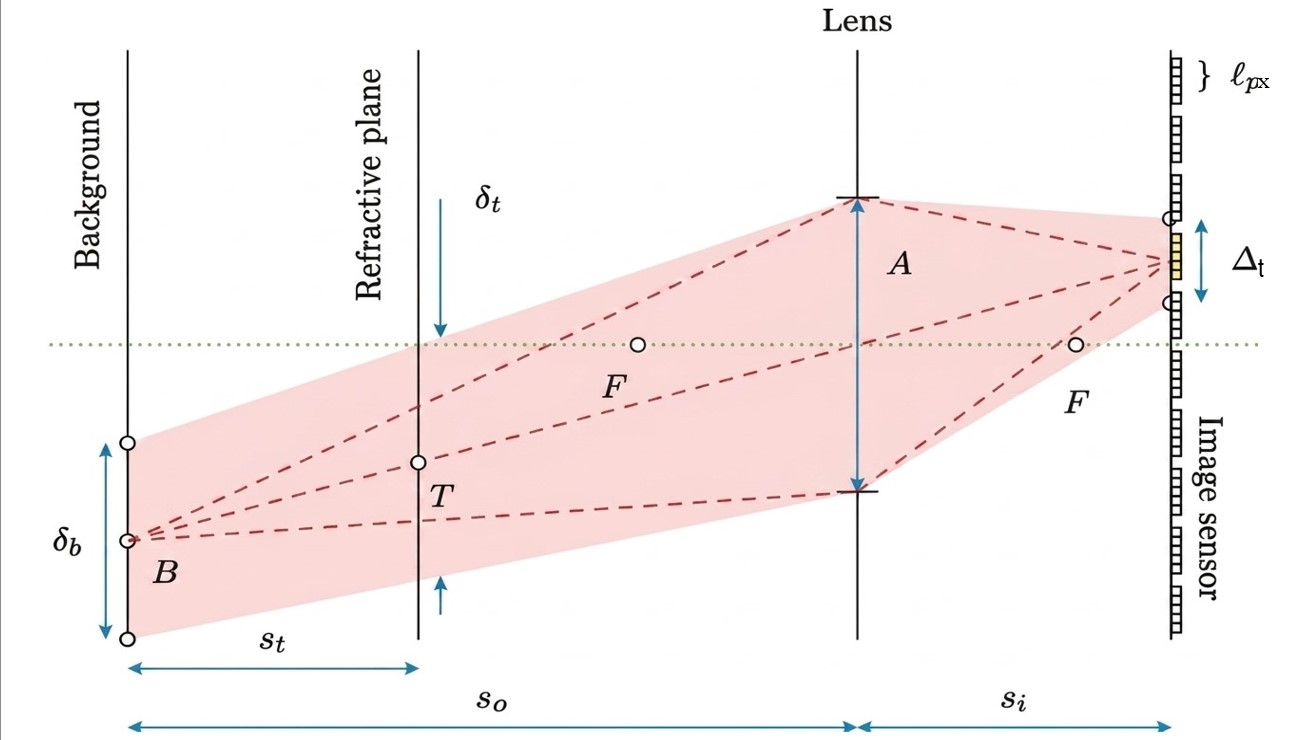
\includegraphics[width=0.8\textwidth]{figures/Gojani cone of light diagram.jpg}
    \caption{Diagram of the cone of light that reaches a length in the sensor $\Delta_t$, this image was used by Gojani et al. to derive his equation for spatial resolution. Credit to Gojani et al. \cite{Gojani&Obayashi}}
    \label{fig: Gojani cone of light}
\end{figure}

\par In Gojani's derivation of the blur circle $\delta_t$, they explicitly call the length in the sensor plane $\Delta_t$ as the "circle of confusion ($CoC$)" \cite{Gojani&Obayashi}. However, Ambiguity arises when they subsequently define it as a sampling cell $\Delta_t = k \cdot l_{px}$, where $k$ is a small integer and $l_{px}$ is the pixel pitch, do not explicitly say how $k$ is computed and fix $\Delta_t$ in the range of 5-50 $\mu$m. Appendix \ref{Appendix: Blurred Object} demonstrates that using Greenleaf's equation for the $CoC$ \cite{Greenleaf1950} to compute $\Delta_t$ places it outside that range for certain applications and yields a blur circle  $\delta_t = 2 \cdot CoC_{obj}$, which is four times the minimum distinguishable feature size $s_{min}$ measured by Schwarz and Braukmann \cite{Schwarz&Braukmann}. Moreover, no systematic experimental validation corroborating Gojani's claims has been found in the literature. Michalski used their formulation and attempted to compare it with the maximum density gradient width of a jet, still it was found to be only in a comparable order of magnitude to the computed value (width of 1.66 mm and $\delta_t$ of 0.86 mm) \cite{Michalski2018}. 

\par Contrasting to Gojani's approach, Schwarz and Braukmann systematically correlated $CoC$ with spatial resolution experimentally \cite{Schwarz&Braukmann}. First, they transferred the $CoC$ to refractive object plane by using a blurred object magnification, thus defining a $CoC_{obj}$ (this transfer was also derived in Appendix \ref{Appendix: Blurred Object}). Then, they obtained the smallest distinguishable size by measuring the contrast in light intensity of bright and dark bars of a resolution target for various optical setups. Schwarz's figure for spatial resolution is thus based on a separability criterion, it defines how close two points may lie before their image is merged. It was found that the minimum discernible feature was around half the $CoC_{obj}$, $s_{min} \approx 0.5 \cdot CoC_{obj}$. 

\par As it has been implicitly mentioned, Schwarz's result and Gojani's formulation are fundamentally different. Gojani derives the blur circle, whereas Schwarz is interested in a separability criterion. Therefore, Schwarz measure should be the radius of the circle derived by Gojani. Gojani's final formulation of $\delta_t$ in equation 12 corresponds to this, thus it is in agreement with Schwarz. However, his reasoning to drop the term containing $\Delta_t$ is weak, given that both terms in his formulation amount to the same value if $\Delta_t = CoC$, as shown by Appendix \ref{Appendix: Blurred Object}.

\par Ultimately, the experimental validation makes Schwarz's formulation the stronger of the two. Additionally, the loose definition of $\Delta_t$ in Gojani's formulation leads to ambiguity that can be interpreted into a result two times larger than the one corresponding to Schwarz's measurements. Since Schwarz's formulation is backed by experimental data, it is stronger than Gojani's and should be used to estimate the optical spatial resolution of a BOS setup. Therefore, the minimum distinguishable feature used for this thesis is the one derived by Schwarz and presented here in equation \ref{equation: smin}.

\par Up to this point, spatial resolution and sensitivity have been described primarily as functions of the optical setup, which governs the level of blur in the test section. However, these performance parameters are also significantly influenced by the choice of post-processing algorithms and hardware. Different image processing techniques can achieve varying levels of sensitivity and spatial resolution when converting captured images into displacement fields. While the characteristics of the background pattern such as speckle size and frequency also limits spatial resolution and influence the choice of post-processing algorithms. Therefore, each must be carefully selected for an experiment \cite{Schmidt2025}. 

\subsection{Imaging hardware and post-processing}
\label{subsection: Image processing}

%Add a picture on image processing?

\par On the imaging hardware level, the main parameter that influences resolution is the pixel density, which quantifies how many pixels correspond to a millimeter in the image. It is related to the magnification but also the size of the sensor and its pixels \cite{Schmidt2025, Gojani&Obayashi}. A smaller pixel size and higher magnification provides a higher pixel density, which means that a smaller feature can be imaged with more pixels, providing more detail. It is worth noting, that it is no use to have a higher spatial distribution of pixels if the blur limits the size of the smallest distinguishable feature. Consequently, an optimization must take place where the optical spatial resolution matches the hardware and post-processing resolution, so that the setup resources are used efficiently. Schwarz et al. make precisely this comparison by expressing both the circle of confusion and the interrogation window in the object domain and evaluating each against the size of the structure under study \cite{Schwarz&Braukmann}.

\par Once the BOS images are taken, they must be processed in a step that converts the recorded images into a displacement field data. The algorithm chosen for it bounds both the accuracy and the spatial resolution of the result. Cross-correlation (CC) was the first method applied to the technique \cite{Raffel2001} and remains the most widely used. Coming directly from its use in PIV, it divides the reference and the deflected image into interrogation windows, and uses a cross-correlation function applied to the intensity distribution of each window pair to find the displacement that best aligns them \cite{Schmidt2025}. One vector is returned per window, so the spacing of the resulting field follows from the window size $W$ and the fractional overlap $o$ as $W(1-o)$, for example, a 64 pixel window at $75\%$ overlap yields a vector every 16 pixels.

\par The inheritance from PIV comes with its drawbacks, Schmidt et al. \cite{Schmidt2025} point out two differences between the applications. Displacements in BOS are of the order of a few pixels rather than the ten to twenty typical of PIV \cite{Schmidt2025, Raffel2015}, so the dynamic range CC is designed to deliver goes largely unused while its penalty in accuracy and resolution is still present. Raffel notes that although displacements below half a pixel can still be determined with high accuracy, the smaller signal leaves BOS with relative errors of the order of 2--3\% of full scale against roughly 1\% for PIV \cite{Raffel2015}. Moreover, the background is manufactured in BOS as a field of discrete bright dots imitating tracer particles, which is not the best suited pattern to resolve a smooth displacement field \cite{Schmidt2025, CakirEtAl}.

\par These shortcomings motivated several alternatives. Iterative least squares (ILS) uses CC to locate the integer-pixel displacement and computes the subpixel part through a separate fit. This improves subpixel accuracy and reduces sensitivity to imaging noise. Optical flow (OF) abandons windows altogether and solves for the whole field at once, returning a vector at every pixel, at a computational cost roughly an order of magnitude above CC. Fourier demodulation (FCD) recovers the deflections from phase shifts in the Fourier domain and is faster than either, but demands a periodic background such as a sinusoid or a checkerboard. On idealized synthetic images OF and FCD reproduce the ground truth almost exactly, while CC and ILS visibly undersample sharp gradients \cite{Schmidt2025}, a ranking supported by Cakir et al. \cite{CakirEtAl}, who report a clear advantage of OF over CC in both accuracy and the range of resolvable density gradient amplitudes on a Prandtl-Meyer expansion fan.

\par Those margins narrow considerably in practice. Schmidt et al. observe that the advantage of a higher-fidelity algorithm is realized mainly when small-scale structures dominate and the images are essentially free of noise, and that defocusing can turn the advantages obsolete by blurring the fine scales out before processing begins \cite{Schmidt2025}. Schwarz et al. reach the same conclusion independently, reporting that in their own evaluations with synthetic BOS images they could not reliably match the resolution and accuracy of a $12 \times 12$ pixel cross-correlation using optical flow \cite{Schwarz&Braukmann}. Since a BOS setup is deliberately defocused on the refractive object, this technicality applies directly. Combined with the periodic pattern FCD demands, which a laser speckle field cannot provide, the computational cost of OF and the absence of both from commercially available packages, the practical balance favors cross-correlation with a potential iterative least squares refinement.

\par Within CC, the interrogation window governs the compromise between robustness and resolution. Indeed, Schwarz et al. name the window size and the geometric blur as the two factors that jointly limit the spatial resolution of a BOS measurement \cite{Schwarz&Braukmann}, so the optical and processing bounds cannot be chosen independently. Small windows are preferred in BOS precisely because the displacements are small \cite{Schmidt2025}, yet a window holding too few features yields an unreliable correlation peak. The minimum window size recommended in the literature ranges from four to five to ten background dots, depending on the author \cite{Schwarz&Braukmann}. Kähler et al. \cite{KahlerEtAl} quantified the resulting limit through the step response width, the smallest separation at which two vectors are genuinely independent, and showed it to grow both with the window size and the diameter of the imaged features. This means that a raise in the overlap produces a denser vector field without improving that independence, so the final window size, and not the vector spacing, is what sets the true spatial resolution of a measurement.

\par The same analysis determines the size of the background features themselves. Reliable subpixel interpolation of the correlation peak requires feature images larger than roughly two pixels. Below that threshold the fit can no longer locate the peak and the estimated displacements collapse toward integer values, an artifact known as peak locking \cite{KahlerEtAl}. Large features are equally unhelpful, since the step response width grows in proportion to their diameter, and once they reach about a quarter of the window size the partial features cut by the window edges degrade the response sharply. Holding the imaged feature between roughly two and five pixels satisfies both bounds. BOS literature converges on the same interval from experience: Raffel \cite{Raffel2015} reports background structures typically imaged at three to five pixels, with two to three preferable but rarely attainable because of diffraction at the small apertures BOS demands. He also cautions that the three-point peak fit inherited from PIV adds noise once the structures grow beyond that. Schwarz et al. quote an optimum dot image of about three pixels and worked at 3.4 to 5 pixels in their own experiments \cite{Schwarz&Braukmann}. For speckle backgrounds the same target applies, Michalski et al. sized their speckles at 61.6~\textmu m to cover roughly four pixels \cite{Michalski2018}. It is this requirement that is sought to be respected by the optical design of Chapter \ref{chapter: methodology}.

\par Processing and optics therefore impose complementary limits on what a BOS measurement can resolve. Neither has confined the technique to a single form: over the past twenty-five years it has been adapted to three-dimensional fields, to scales ranging from millimeters to aircraft in flight, and to backgrounds of very different kinds. Those developments are reviewed next.

\subsection{Variants of BOS}
\label{subsection: Variants of BOS}
\par Since BOS was introduced 25 years ago, the technique has not remained static, various authors have worked on modifications that enabled its application where it would be impractical to do so with the standard method. These developments were surveyed by Raffel \cite{Raffel2015} at the fifteen-year mark and, more recently, by Schmidt et al. \cite{Schmidt2025} across the full twenty-five years. A significant evolution was the development of tomographic BOS, which combines multiple camera perspectives to reconstruct three-dimensional density fields \cite{TomographicBOS, Raffel2015}. This method was demonstrated in applications ranging from supersonic wind tunnel tests to combustion imaging, and has since become the principal route to unsteady structures in variable-density flows \cite{Schmidt2025}. For setups where multiple cameras are unavailable, plenoptic BOS offers an alternative by capturing various perspectives from a single camera through a micro-lens array, enabling independent refocusing at different planes along the line of sight from a single image \cite{PlenopticBOS}. These modifications have greatly expanded the scope of BOS applications beyond single 2D gradient imaging.

%Add a picture here on one of these emethods

\par Other studies have focused on the limits of scaling BOS. At small scales, telecentric BOS addresses the geometric blur inherent to conventional setups through collection of parallel light rays onto the sensor \cite{TelecentricBOS}. This way perspective distortion is reduced and spatial resolution improved for fine-scale measurements. Van Hinsberg and Rösgen \cite{vanHinsberg2014} developed what they called Near-Field BOS. They modified the correction factor in the BOS relation presented by Dalziel et al. \cite{Dalziel2000} so that reliable densities can still be recovered when the background sits closely behind the flow. This removes the usual requirement for a large background-to-object distances. At larger scales, airborne BOS (AirBOS) has enabled schlieren imaging of supersonic aircraft in flight by using the Earth's natural surface texture as a background \cite{AirBOS, AirBOS2}, an approach whose viability rests on selecting terrain whose natural structures image at the same few-pixel scale demanded of a printed pattern \cite{Raffel2015, Schmidt2025}. Another method (BOSCO) has used celestial objects such as the Sun for the same purpose \cite{BOSCO}. Outdoor explosive and ballistic tests have  also leveraged natural backgrounds and zebra board patterns to visualize shock wave propagation over fields of view inaccessible to laboratory optics \cite{ExplosionsBOS, Schmidt2025}. As a result, BOS can be applied in contexts where normal schlieren would have been impractical as it would need unreasonably heavy and large optical elements.

\par For high-speed applications that demand high luminous intensity, developments have been made in background illumination strategies. Back-illuminated transparent patterns and retroreflective sheeting with co-linear illumination have both been demonstrated as effective solutions in large-scale ground test facilities \cite{RBOS, BackIluminatedBOS}. As Raffel \cite{Raffel2015} mentions, the methods are motivated by the fact that a small aperture is wanted to limit blur but starves the sensor of light, while short exposures are wanted to limit motion blur. Therefore, retroreflective material is valuable precisely because its on-axis return does not obey the inverse-square law that penalizes a diffuse background, allowing for better contrast. The same design pressure has driven sensor technology, from pulsed and high-framing-rate BOS \cite{Raffel2015} to event-based cameras, which record only pixel-level brightness changes, allowing them to reach kHz rates at a fraction of the illumination power and cost \cite{Schmidt2025}. More recently, laser speckle has been proposed as a background source due to its high intensity and the always-in-focus nature of the speckle pattern at the sensor \cite{Meier&Roesgen2013}, properties that form the conceptual basis for the SBOS method investigated in this thesis.

\section{Laser Speckled Background Oriented Schlieren}
\label{sectio: Laser Speckled BOS}
\par Laser-Speckled Background Oriented Schlieren is based on the same principles of BOS, with the distinct difference that a laser speckled pattern is used as reference instead of a physical background pattern. The speckle pattern is a result of the constructive and destructive interference caused by the interaction of scattered wavefronts originating from a previously collimated coherent light source, which arrive at the sensor with random phase differences. This interference pattern has been extensively investigated since the 1960s \cite{NikitaFominBook, Goodman2020} and has found applications in diversified fields such as the imaging of blood flow in medical fields \cite{Boas&Dunn2010}, non destructive analysis of structural materials through shearography \cite{Hung&Ho2005} and the study of density gradients using laser speckled interferometry \cite{Debrus1972}. However, the first reported use of a laser speckle pattern as a BOS background was by Meier and Rösgen in 2013 \cite{Meier&Roesgen2013}. It can be said then that SBOS is a relatively new development and being this recent, it is yet to be largely applied and studied, presenting the opportunity for novel and interesting developments.

\par Speckle creation has been extensively treated by Goodman \cite{Goodman2020} and its application to fluid mechanics measurements by Fomin \cite{NikitaFominBook}. As aforementioned, the speckles are created when light gets scattered by a surface rougher than its wavelength, which randomly changes the amplitude and the optical path length of the scattered rays and thus creates an interference pattern. This surface can be a rough projection plane or a diffuser such as a ground glass. The speckles can either be objective, when the scattered light propagates freely to an observation plane; or subjective, when it is collected by a lens. It is worth highlighting that speckle creation is random at its core \cite{Cloud2007, Goodman2020}. As a consequence, the theoretical mathematical treatment of this phenomenon involves complex Fourier analysis and statistics, which were considered out of scope. This thesis will treat more on the practical aspects of speckle generation and try to develop practical guidelines for its use.

\par The work of Meier and Rösgen \cite{Meier&Roesgen2013} introduced SBOS and showed that using a laser speckled background greatly expands the design space of a BOS experimental setup. By creating subjective speckles, the exit pupil of the imaging system itself can be regarded as the effective scattering spot \cite{Goodman2020}. Consequently, the speckles stay sharp at any virtual position the camera has its focus on. This permits the positioning of the pattern to be virtually anywhere along the laser beam, be it in front of the refractive object, inside of it, behind it, or even beyond the scattering plane. Consequently, optical arrangements that would be impossible in conventional BOS become feasible with SBOS. A picture of their experimental setup can be seen in Figure \ref{fig: SBOS Meier and Roesgen}.

\begin{figure}[h]
    \centering
    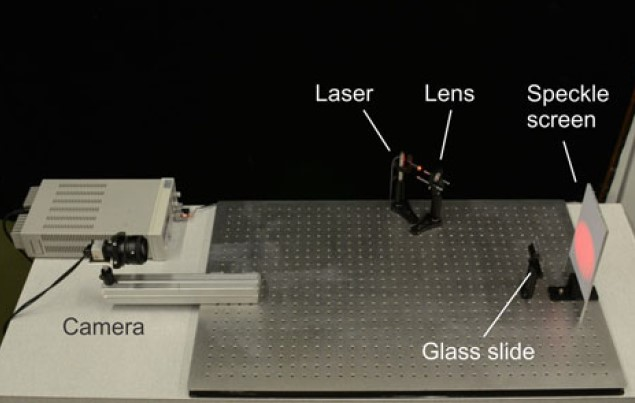
\includegraphics[width=0.6\textwidth]{figures/Meier and Roesgen single pass setup.jpg}
    \caption{Experimental SBOS setup (single pass) used by Meier and Rösgen \cite{Meier&Roesgen2013}}
    \label{fig: SBOS Meier and Roesgen}
\end{figure}

\par These new optical configurations promise great benefits compared to standard BOS \cite{Meier&Roesgen2013}. By focusing the camera in front of the test section, a larger increase in sensitivity can be achieved while maintaining the same spatial resolution. Positioning the focus beyond the physical position of the screen allows for larger effective defocusing distances while maintaining the screen close to the test section, which greatly reduces the physical size of the setup. Focusing the camera inside the test section improves the spatial resolution; the implications for image quality and sensitivity, however, are not clear. Meier and Rösgen also developed the double-pass mode, where the laser beam is directed coaxially with the camera through the test section, effectively doubling the sensitivity by capturing the deflection of both the illumination beam and the imaging path. The ability to choose among these optical configurations alleviates the constraints between sensitivity and spatial resolution present in standard BOS, allowing for a much more optimized optical setup. 

\par Furthermore, replacing the conventional printed background with a laser-generated speckle pattern offers advantages in terms of background quality and spatial frequency content. Unlike physical background patterns, whose feature size is constrained by printing and manufacturing limitations, the minimum speckle diameter is only limited by the Rayleigh diffraction criterion \cite{Barker&Fourney}. If the interference pattern becomes diffraction limited due to the camera aperture, it will be only constrained by the laser wavelength, the f-stop number and the camera magnification. Consequently, SBOS can produce significantly finer background structures, providing higher spatial-frequency information for image correlation and potentially improving the spatial resolution.

\par After the work of Meier and Rösgen, only a limited number of studies have explored SBOS experimentally. Bühlmann \cite{Buhlmann2020} employed the technique in the tomographic imaging of a heated jet near a wall where the laser-speckle was projected as a background. His measurements highlight the potential of SBOS as they would have been unfeasible with conventional BOS. Michalski et al. \cite{Michalski2018} applied the method using the in-focus plane in front of the refractive object to obtain the calorimetry of an electrical spark discharge. In contrast to the previously mentioned works that used a scattering screen, Michalski et al. used a ground glass diffuser to scatter the laser beam and pointed it directly to the camera sensor, much similar to the setup used by Debrus on speckle interferometry \cite{Debrus1972} as it can be seen in Figure \ref{fig: SBOS setup illustrated}. Their work also rigorously quantified the method's uncertainties and compared its accuracy with standard BOS, which will be discussed in the next section. Nakamura et al. \cite{Nakamura2021} also employed laser speckles in a different way to develop a methodology intended to compute the depth location of refractive structures inside the test section and used a compressible jet to demonstrate it. Both Nakamura's and Michalski's work highlight the usefulness of SBOS for imaging fast phenomena with low signal-to-noise ratio. These studies demonstrate the method's potential, nevertheless, most of its developments have originated from a small number of research groups. Consequently, important questions regarding implementation, uncertainty, spatial resolution, and applicability in demanding environments remain insufficiently explored.

\begin{figure}[htbp]
    \centering
    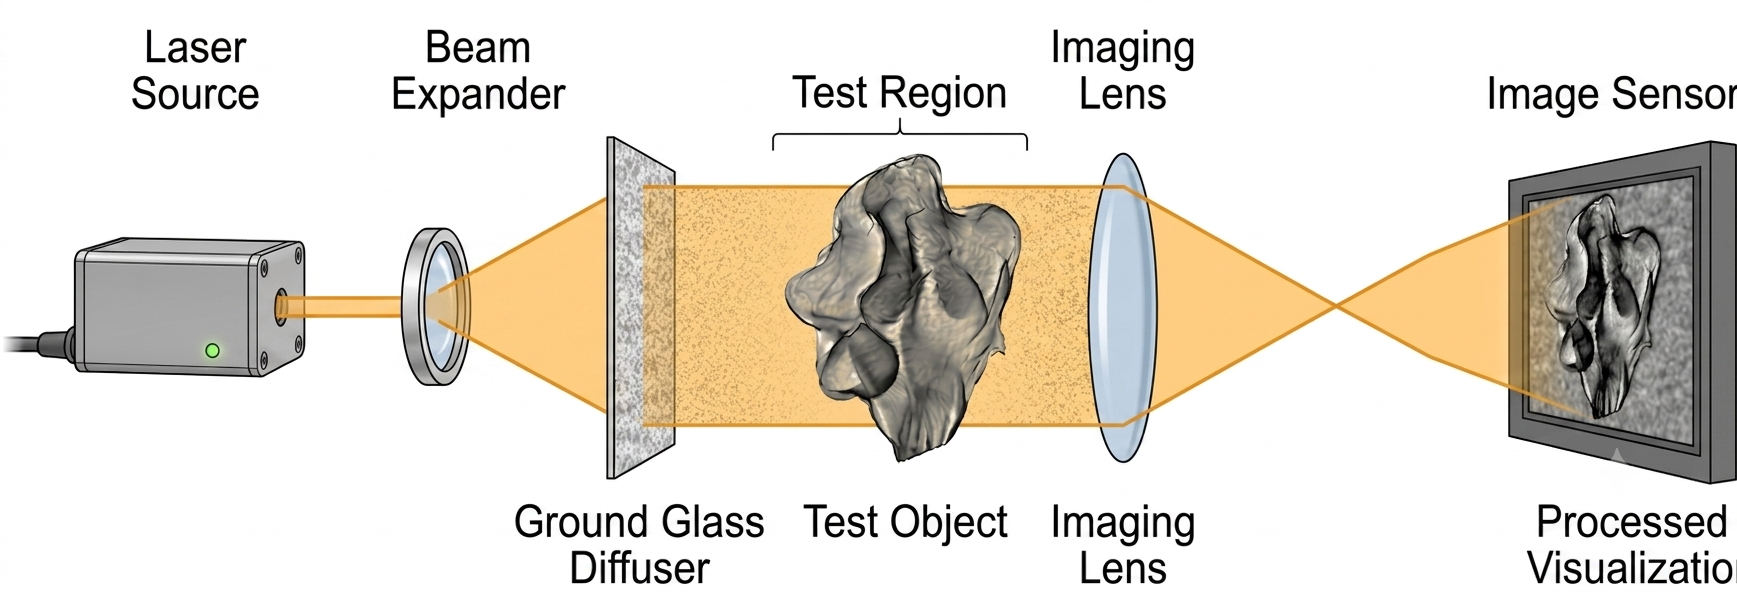
\includegraphics[width=0.6\textwidth]{figures/SBOS setup ilustrated.png}
    \caption{Illustration of a SBOS setup using ground-glass-diffused laser speckles, similar to Michalski's setup \cite{Michalski2018}}
    \label{fig: SBOS setup illustrated}
\end{figure}

\subsection{Limitations, accuracy and uncertainty of SBOS}

\par Despite its advantages, SBOS presents some constraints and drawbacks that must be considered in its implementation. Some of these are shared with BOS such as spatial resolution and sensitivity constraints due to the chosen processing algorithms and hardware. Others are exclusive to SBOS, such as higher complexity and possible decorrelation problems. This subsection will discuss how literature treats these limitations and how it provides a comparison of the method’s accuracies and uncertainties with standard BOS.

\par A natural complication of SBOS is the increased complexity that comes with using a laser instead of a physical background. It requires laser compatible lenses, more optical elements, special care when handling and maintaining the setup and additional safety concerns as the laser presents a hazard at high energy settings. By implementing the method, a trade-off must be made between the increased complication and the gains in resolution and sensitivity; this will be treated in more depth in the methodology chapter.

\par It is also worth noting that there have been two ways in the literature to generate the speckle pattern and both have been used successfully for SBOS. It is possible to classify them into projected speckles employed by Bühlmann \cite{Buhlmann2020} and Meier and Rösgen \cite{Meier&Roesgen2013}, and directed speckles used by Michalski et al. \cite{Michalski2018} and Nakamura et al. \cite{Nakamura2021}. It is not clear which one of them is more effective in generating speckles, that is, what the drawbacks and advantages of each approach are. It might be only a matter of convenience when only one optical access is available, maybe one of the methods presents a more uniform distribution of speckles or is more prone to decorrelation than the other. Given the lack of literature on the topic, it would be interesting to test them both and compare them.

\par Decorrelation is the failure to correlate the background shift with the reference pattern and it's a phenomenon that might arise when using a laser speckled pattern as background. Bühlmann encountered this as a substantial problem on his projected laser speckle setup, which required him to use large cross-correlation windows and apply corrections for the pattern shift \cite{Buhlmann2020}. Li and Chiang have researched decorrelation effects for laser speckle interferometry and concluded that the main sources of the effect are surface tilt, out-of-plane displacement and lens aberration \cite{Li&CHiang1986}. Meier and Rösgen have also mentioned linear induced errors due to projecting surface tilt, so it could be that using projected speckles, like in Bühlmann’s setup, makes the method more prone to decorrelation \cite{Meier&Roesgen2013}. Neither Nakamura et al. nor Michalski et al. have reported the issue in their direct laser-speckle setups, which suggests that the effect could be mitigated by this approach \cite{Nakamura2021, Michalski2018}.

\par Regarding the accuracy of the technique, both Michalski and Nakamura quantified errors in their applications \cite{Michalski2018, Nakamura2021}. Michalski et al. validated their implementation with a CO$_2$  jet and obtained a mean density for the core $0.8\% \pm 0.9\%$ lower than expected, yielding a $0.3\% \pm 0.3\%$ error for the final measured CO$_2$ density. Nakamura et al. described an approximated error of $10\%$ on their method to identify the depth position of refractive objects, but did not show the errors of their density field. Compared to BOS, whose measurement error has been found to be in the order of $2-3\%$ of the full scale by Raffel\cite{Raffel2015} and Elsinga et al. \cite{Elsinga2004} reporting an accuracy of around $2\%$ against theory for a Prandtl--Meyer expansion fan, SBOS applied by Michalski et al. performs well in terms of accuracy.

\par Uncertainty and noise are also important aspects to ascertain in experimental techniques. Michalski et al. \cite{Michalski2018} and Meier and Rösgen \cite{Meier&Roesgen2013} mention that the increased sensitivity of SBOS also makes it more prone to noise from vibration coming from setup equipment. Moreover, noise could come intrinsically from the camera sensor, room temperature gradients and even the image processing algorithm. Michalski et al. estimated the total uncertainty in their setup, quantifying partial uncertainties from the integration method, magnification, defocusing distance, cross-correlation, tomographic reconstruction and white noise, reaching a final value of $6.2\%$. In this project, the uncertainty sources of the designed setup will be documented in Chapter \ref{chapter: Experimental Setups} and their impact quantified in the results.

\section{Research Gap}

\par The literature review reveals that SBOS is a promising, but not yet mature, technique. While Meier and Rösgen established its conceptual foundation and demonstrated its advantages over standard BOS \cite{Meier&Roesgen2013}, the subsequent body of work remains sparse, originating largely from a small number of research groups and covering a narrow range of applications. This contrasts sharply with the extensive and well-validated literature surrounding conventional BOS. Three clusters of open questions emerge from this review. First, no systematic implementation guidelines exist for SBOS setup design. The sensitivity-resolution trade-off is well characterized for BOS, but whether and how those relationships translate to SBOS configurations, particularly for unusual background placements, has not been thoroughly addressed. Second, uncertainty quantification remains incomplete. Michalski et al. provide the most rigorous treatment to date \cite{Michalski2018}, but their setup is specific enough that their uncertainty budget cannot be straightforwardly transferred to other configurations. Third, the behavior of SBOS in demanding high-speed wind tunnel environments is entirely unexplored, leaving open questions about decorrelation, vibration sensitivity, and optical feasibility under those conditions.

\par Together, these gaps mean that a researcher wishing to implement SBOS today would find no coherent roadmap to follow. The present thesis addresses this by designing, building, and systematically investigating an SBOS setup, using a high-speed wind tunnel application as the target demonstration case. The specific research questions motivating this work are stated in Chapter \ref{chapter: introduction}.
\chapter{Practical Design Guidelines of BOS Setups}
\label{chapter: methodology}

This chapter describes the methodology used to design the experimental setups. First, a brief description of the geometry of two optical setups is presented, one typical to BOS and another exclusive to SBOS. The standard BOS setup, discussed in subsection \ref{subsection: standard BOS geometry}, places the in-focus plane on the background reference behind the refractive object, as the conventional configuration described in the literature. Subsection \ref{subsection: Negative defocus geometry} then introduces the negative defocus setup, a configuration made possible only by SBOS, where the in-focus plane is positioned in front of the test subject. For both geometries, the governing equations relate performance parameters such as sensitivity, spatial resolution and speckle size to physical setup variables.

A design strategy was then envisioned to define the setup variables and explore how they interact across the feasible design space. Rather than solving the system for a single configuration, a MATLAB script was developed to compute the full set of variables X = ($S, s_{min}, \Delta s, d_f, Z, M, CoC, m$) for a range of combinations of the parameters P = ($f_\#, l, f$). This design space exploration, presented in section \ref{section: Design Strategy}, allows the main trends that govern the optical setup to be visualized through surface maps and provides insight into how focal length, defocus distance and f-stop number affect the trade-off between sensitivity and spatial resolution. The strategy is applied first to the SBOS configuration (subsection \ref{subsection: Surface Maps for SBOS}), then to the standard BOS configuration (subsection \ref{subsection: Surface maps for BOS}) for comparison, before the effect of the object field of view is examined in subsection \ref{subsection: Effets of FoV}. Section \ref{section: Summary of Practical Guidelines} then collects the outcomes of this exploration into a single set of practical design guidelines. Together, these sections establish the reasoning behind the final design choices used in the experimental setups described in Chapter \ref{chapter: Experimental Setups}.

\section{Geometries of a SBOS optical setup}
\label{section: Geometries of a SBOS optical setup}
Laser speckled background oriented schlieren opens the possibility of novel and unusual optical configurations that would be otherwise unfeasible for a standard BOS setup. A description of the geometry of a normal BOS configuration is given below, followed by the detailing of the negative defocus position. This section presents and compares the equations used for both setups. These formulas will be used to assess the difference in performance of a standard BOS setup and an exclusive SBOS configuration.

\subsection{Positive defocus setup}
\label{subsection: standard BOS geometry}
\par A positive defocus setup is the standard BOS configuration, where the in-focus plane is on the background reference behind the refractive object, as shown in Figure \ref{fig: Geometry BOS}. The Figure displays relevant distances for the design of the setup: $d_f$ corresponds to the distance of the in-focus plane to the camera lens, $m$ is the distance between the lens and the refractive object and $l$ is the distance between the test section and the in-focus plane, also called defocus distance. $Z$ is the distance between the lens and the formed image, following the ideal lens relationship. The latter is important if a single converging lens is used to collect light, however it is not so relevant when compound lenses such as the ones present on modern cameras are used. Other parameters to be defined are: the magnification $M$ of the object in the image plane, the lens focal length $f$ and the camera f-stop number $f_\#$. All these variables will be defined by the equations below.

\begin{figure}[htbp]
    \centering
    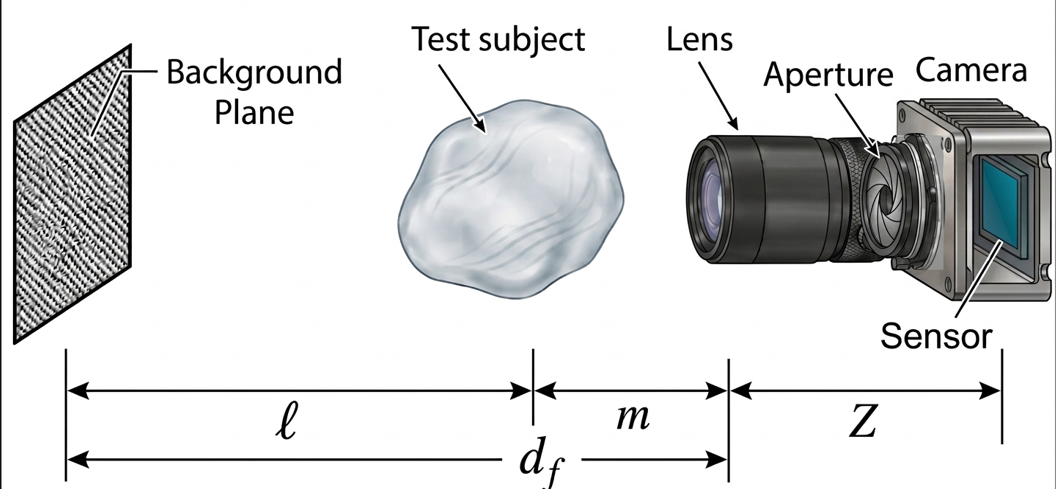
\includegraphics[width=0.6\textwidth]{figures/BOS setup.png}
    \caption{Geometry of a standard BOS Setup (positive defocus) }
    \label{fig: Geometry BOS}
\end{figure}

\par Equation \ref{equation: df} derives directly from Figure \ref{fig: Geometry BOS} and relates the distances $m, d_f$ and $l$. The defocus distance $l$ is measured from the refractive object to the in-focus plane, so it is treated as positive when the in-focus plane lies behind the object, and negative when it lies in front of it. The same equation therefore describes both geometries, with only the sign of $l$ changing.

\begin{equation}
    \label{equation: df}
    d_f = m + l
\end{equation}

\par For a first preliminary sizing, let's consider the camera lens as ideal. This permits the use of the gaussian thin lens equation (equation \ref{equation: Thin Lens equation}) and the coupled definition of magnification (equation \ref{equation: M}). In these equations, the object positioned at a distance $d_f$ from the lens is in focus and has its image at a distance $Z$ behind the lens with a magnification $M$. This formula comes with a specific convention regarding the sign of $M$, where negative $M$ corresponds to an inverted image and a positive to an upright image. Since a camera is being used, only the inverted image is going to be considered and for the sake of convenience this will be taken as positive. The camera also implies that $d_f > f$, as no image can form on the imaging sensor otherwise.

\begin{equation}
    \label{equation: Thin Lens equation}
    \frac{1}{f} = \frac{1}{d_f} + \frac{1}{Z}
\end{equation}

\begin{equation}
    \label{equation: M}
    M = \frac{Z}{d_f}
\end{equation}

As discussed in chapter \ref{chapter: LiteratureReview} Schwarz et al. \cite{Schwarz&Braukmann} and Gojani et al. \cite{Gojani&Obayashi} have drawn guidelines for the practical design of a BOS optical setup highlighting the importance of the sensitivity and spatial resolution. Sensitivity $S$ can be written as shown in equation \ref{equation: S BOS}, while the minimum distinguishable feature $s_{min}$ defined by Schwarz et al. \cite{Schwarz&Braukmann} is given by equations \ref{equation: CoC BOS} and \ref{equation: smin}.
%while the spatial resolution $s_{min}$ defined by Gojani et al. is written by equations \ref{equation: CoC BOS} and \ref{equation: d_av BOS} .

\begin{equation}
    \label{equation: S BOS}
    S = \frac{\Delta y}{\epsilon} = lM 
\end{equation}

\begin{equation}
    \label{equation: CoC BOS}
    CoC = \frac{lfM}{f_\#m}
\end{equation}

\begin{equation}
    \label{equation: smin}
    s_{min} = \frac{CoC}{2 \cdot M_{obj}}
\end{equation}

%\begin{equation}
%\label{equation: d_av BOS}
%    s_{min} = \frac{lM}{f_\#(M+1)} + \frac{CoC}{M} \left( 1 - \frac{l}{d_f}\right)
%\end{equation}
\par In equation \ref{equation: smin}, $M_{obj}$ is the blurred object magnification, which is defined by equation \ref{equation: M obj}.

\begin{equation}
    \label{equation: M obj}
    M_{obj} = \frac{L_{sens}}{L_{FoV_{obj}}}
\end{equation}

Equation \ref{equation: M obj} relates the field of view of the object and the camera sensor dimension. In the literature \cite{Schmidt2025, Schwarz&Braukmann}, many authors define the focal length $f$ by choosing a desired field of view of the object. They utilize equation \ref{equation: LFoVobj simplified} which is derived through the ideal lens equation and the definition of magnification. Thus it makes the fundamental assumption that the object is in focus as the ideal lens equation only applies to in-focus objects. Since the refractive object is out of focus, the assumption is fundamentally wrong and another equation must be derived to connect the lens' focal length to the blurred object's dimension. Geometry can be used to derive equation \ref{equation: LFoVobj BOS} without relying on the ideal lens relationship, the derivation can be found on Appendix \ref{Appendix: Blurred Object}.

\begin{equation}
    \label{equation: LFoVobj simplified}
    f = \frac{L_{sens}m}{L_{FoV_{obj}}+L_{sens}}
\end{equation}

%\par If the field of view of the object is small, blur plays a bigger role. The refractive object size differs from the one obtained before, which risks setting up a field of view that is too small than the one desired, consequently, losing information. In order to compute the $L_{FoV_{obj}}$ for small field of views, the same rationale used by Gojani et al. \cite{Gojani&Obayashi} can be used to derive equation \ref{equation: LFoVobj BOS}. Using this method, the test subject dimension is defined through the expanded cone of light that reaches the sensor screen. This way, the field of view of the captured object is more accurately estimated as it considers all the light that comes from the test section and reaches the sensor. The derivation of this equation can be found in the appendix.

\begin{equation}
    \label{equation: LFoVobj BOS}
    L_{FoV_{obj}} = \frac{m \cdot L_{sens}}{f(M+1)}
\end{equation}

%\par Since this project will test the standard BOS setup using laser speckles, the last equation is the Rayleigh diffraction limit, which is used to estimate the minimum speckle size $\Delta s$ \cite{Barker&Fourney}.

\subsection{Negative defocus setup}
\label{subsection: Negative defocus geometry}
Figure \ref{fig: SBOS with negative l} describes the geometry of a SBOS setting with negative defocus distance, which means that the in-focus plane is in front of the test subject. All the equations from the previous section remain valid in this case, that is, equations \ref{equation: df}, \ref{equation: Thin Lens equation}, \ref{equation: M}, \ref{equation: S BOS}, \ref{equation: CoC BOS}, \ref{equation: smin} and \ref{equation: LFoVobj BOS}. The single difference is that $l$ is now negative, so that equation \ref{equation: df} places the in-focus plane in front of the refractive object, as shown in Figure \ref{fig: SBOS with negative l}.
 
\begin{figure}[htbp]
    \centering
    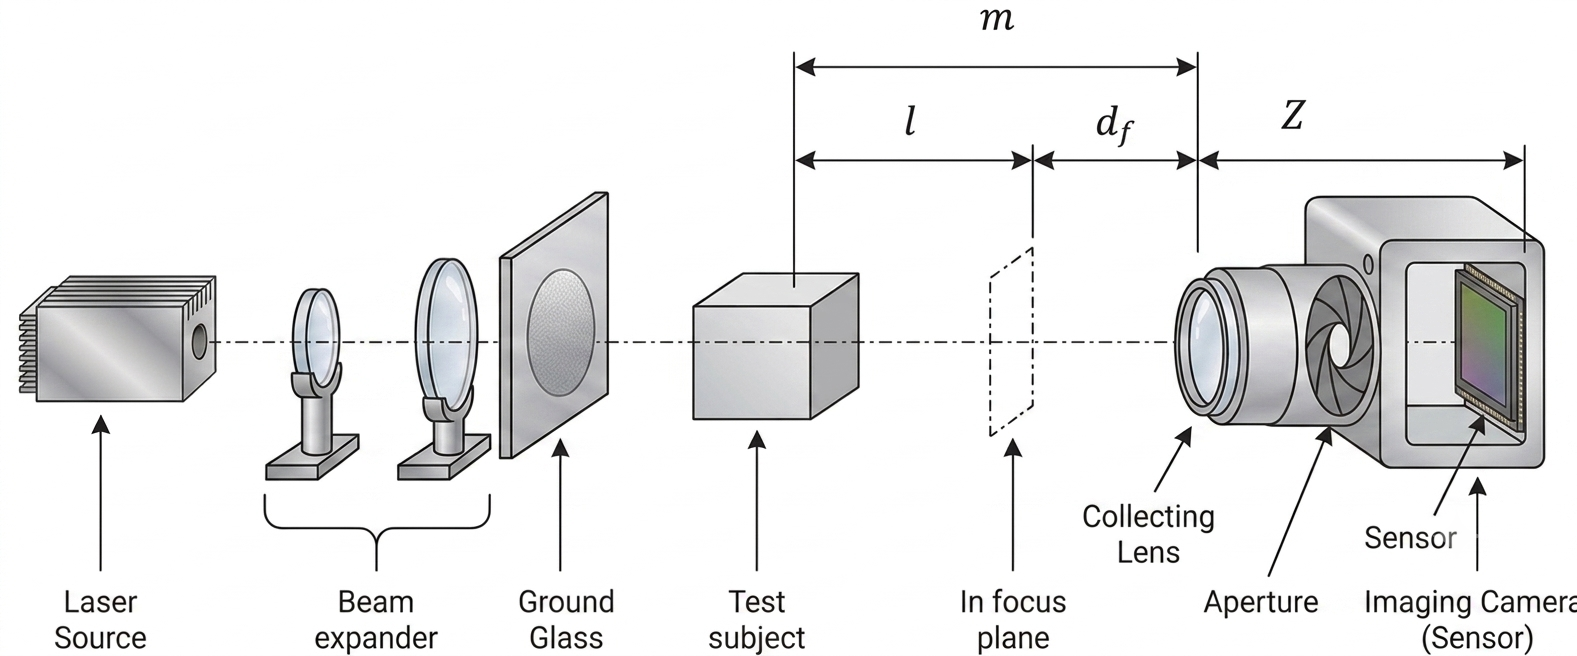
\includegraphics[width=0.6\textwidth]{figures/SBOS with negative l.png}
    \caption{Geometry of a SBOS setup with in-focus plane before the test subject (negative defocus) }
    \label{fig: SBOS with negative l}
\end{figure}

\par Another difference from BOS to SBOS is the speckle generation. Barker and Fourney \cite{Barker&Fourney} have used the Rayleigh limit to quantify the minimum speckle size when working with laser interferometry, the equation is presented as equation \ref{equation: Rayleigh Limit}.

\begin{equation}
   \label{equation: Rayleigh Limit}
   \Delta s = 1.22 \lambda f_\#(1+M)
\end{equation}


\par It has been mentioned in chapter \ref{chapter: LiteratureReview} that this configuration provides a better sensitivity for the same spatial resolution than standard BOS, this might be explained through a careful analysis of the setup geometry and the equations that govern it. In equation \ref{equation: S BOS}, $S$ is directly proportional to $M$, while in equation \ref{equation: M}, $M$ is inversely proportional to $d_f$. Comparing Figure \ref{fig: Geometry BOS} and Figure \ref{fig: SBOS with negative l}, it is clear that for the same defocus distance, $d_f$ is smaller in the latter case. Consequently, $M$ is larger and the sensitivity is higher. However, since $CoC$ also depends on $M$, it is not immediately obvious whether the gain in sensitivity is offset by the additional blur.
\section{Sensitivity-Resolution Ratio}
\label{section: Sensitivity-Resolution Ratio}
The dilemma of increasing sensitivity through magnification but also increasing blur can be solved by relating sensitivity and spatial resolution directly. Using the definition of $s_{min}$ in equation \ref{equation: smin} and substituting the circle of confusion (Eq. \ref{equation: CoC BOS}) yields Eq. \ref{equation: smin expanded}.

\begin{equation}
    \label{equation: smin expanded}
    s_{min} = \frac{l f M}{2 f_\# \, m \, M_{obj}}
\end{equation}

\par The field of view relation of Eq. \ref{equation: LFoVobj BOS} can be rewritten as $m M_{obj} = f(1+M)$, which leaves Eq. \ref{equation: smin compact}. Recognizing $lM$ as the sensitivity (Eq. \ref{equation: S BOS}), the ratio between the two performance parameters reduces to Eq. \ref{equation: S over smin}.

\begin{equation}
    \label{equation: smin compact}
    s_{min} = \frac{lM}{2f_\#(1+M)} = \frac{S}{2f_\#(1+M)}
\end{equation}

\begin{equation}
    \label{equation: S over smin}
    \frac{S}{s_{min}} = 2f_\#(1+M)
\end{equation}

\par Equation \ref{equation: S over smin} shows how the sensitivity-resolution trade-off is locked by the magnification and f-stop number. Since the negative defocus configuration allows for higher magnification, a larger ratio is achieved. This means that the sensitivity will grow larger than spatial resolution and a better trade-off is reached. As an example, for $f = 0.1$ m, $|l| = 0.1$ m, $f_\# = 16$ and $L_{FoV_{obj}} = 2$ cm, the positive defocus solution gives $M = 0.47$ and $S/s_{min} = 47$, while the negative defocus solution gives $M = 1.06$ and $S/s_{min} = 66$: the sensitivity rises by a factor of $2.2$ and $s_{min}$ by a factor of $1.6$, a net gain of roughly $40\%$ in the trade-off.

\par Another consequence is that the f-stop offers a convenient means of improving the sensitivity-resolution trade-off. Contrary to the magnification that, given a fixed field of view, is modified by the defocus distance and camera focal length; the f-stop is easily modifiable by reducing the lens aperture diameter without the need to change any other parameter in the optical setup. This comes with two caveats, as an increase in the f-stop decreases the amount of illumination in the camera sensor, reducing contrast; and it increases the minimum speckle size through Eq. \ref{equation: Rayleigh Limit}.

\par Moreover, it is worth noting that equation \ref{equation: S over smin} is bound by the same variables as equation \ref{equation: Rayleigh Limit} once the laser is selected. Since $\Delta s$ must be kept between 2 and 5 pixels for optimal cross-correlation \cite{KahlerEtAl}, the sensitivity-resolution ratio is confined to a fixed achievable interval. This is not a hard constraint, however, as the speckle size could be bigger than 5 pixels if the CC interrogation window is large enough, with the downside of decreased spatial resolution.

\par The relations derived in this subsection establish how the performance parameters are coupled, but not where in the design space a suitable configuration lies. The next section first shows how the system could be solved for a given specification, then explores the design space numerically. Surface maps are used to show how sensitivity, spatial resolution, speckle size and the setup distances respond to $f$, $l$ and $f_\#$, and how the trends seen there are the graphical counterpart of Eq. \ref{equation: S over smin}.

\section{Design Strategy}
\label{section: Design Strategy}
\par Through the equations derived in the previous sections, a system can be solved to define the geometric aspects of a BOS and SBOS optical arrangement. The sensitivity $S$ and the minimum distinguishable feature size $s_{min}$ are chosen from the requirements of the application, $L_{sens}$ is restricted by the camera and $L_{FoV_{obj}}$ is set by the object of study. Since the f-stop is a discrete variable depending on the camera lens hardware that is mostly independent of other variables, it is also specified as an input. This way, equations, \ref{equation: df},
\ref{equation: Thin Lens equation}, \ref{equation: M}, \ref{equation: S BOS}, \ref{equation: LFoVobj BOS} and \ref{equation: S over smin} form a system of six equations and six unknowns $M$, $l$, $d_f$, $m$, $f$ and $Z$, which admits a unique solution. The circle of confusion and the speckle size then
follow from equations \ref{equation: smin} and \ref{equation: Rayleigh Limit}. The latter must be  verified at the end to ensure the speckle size is in the range of 2-5 pixel, to achieve optimal cross-correlation. 

It is also interesting to follow the inverted direction of the solution and assess how the performance parameters change for different optical arrangements. A MATLAB script was written that would solve the system for a given combination of P = ($f_\#,l,f$) and compute X = ($S,s_{min},\Delta s,d_f,Z,M, m, CoC$). A design space exploration was conducted where the parameters P were varied within feasible ranges and the system solved for each combination. The data collected allowed the construction of surface maps that permitted the visualization of the main trends permeating the design space. With this script at hand, it is possible to select the design point that gives the sensitivity, field of view and spatial resolution desired for a given application. 

\subsection{Surface Maps for negative defocus setup}
\label{subsection: Surface Maps for SBOS}
\par Surface Maps for each variable in X were obtained to better understand the system at hand. This section will show and discuss the main trends in sensitivity, spatial resolution, $M, m, d_f$ and speckle size $\Delta s$, aiming to obtain a better preliminary insight on how to build an optimal negative defocus SBOS setup. For the sake of convenience, the maps presented here only deal with the absolute value of $l$. Moreover, $Z$ and $CoC$ have been omitted because the concept of $s_{min}$ encapsulates $CoC$, and $Z$ is not relevant for a setup with compound camera lenses. The pixel density and $L_{FoV}$ for the in-focus plane have also been computed and will be helpful for the validation of the design strategy during the first experimental campaign, information on them can be found in Appendix \ref{Appendix: Pixel density and FoV maps}. For this first iteration, $L_{FoV_{obj}}$ was set to 2cm, $\lambda = 632.8$nm, pixel size equal 6.5 $\mu$m and the camera sensor has 2560x2160 pixels, resulting in $L_{sens} = 1.4$ cm. Figure \ref{fig: S and dav design surfmap SBOS} shows surface maps of Sensitivity and $s_{min}$ given a range of P. The colored isolines are illustrative reference contours and do not correspond to a selected design point: the red isoline marks $s_{min} = 0.0004$ m and the white one $S = 0.02$ m.

\begin{figure}[htbp]
    \centering
    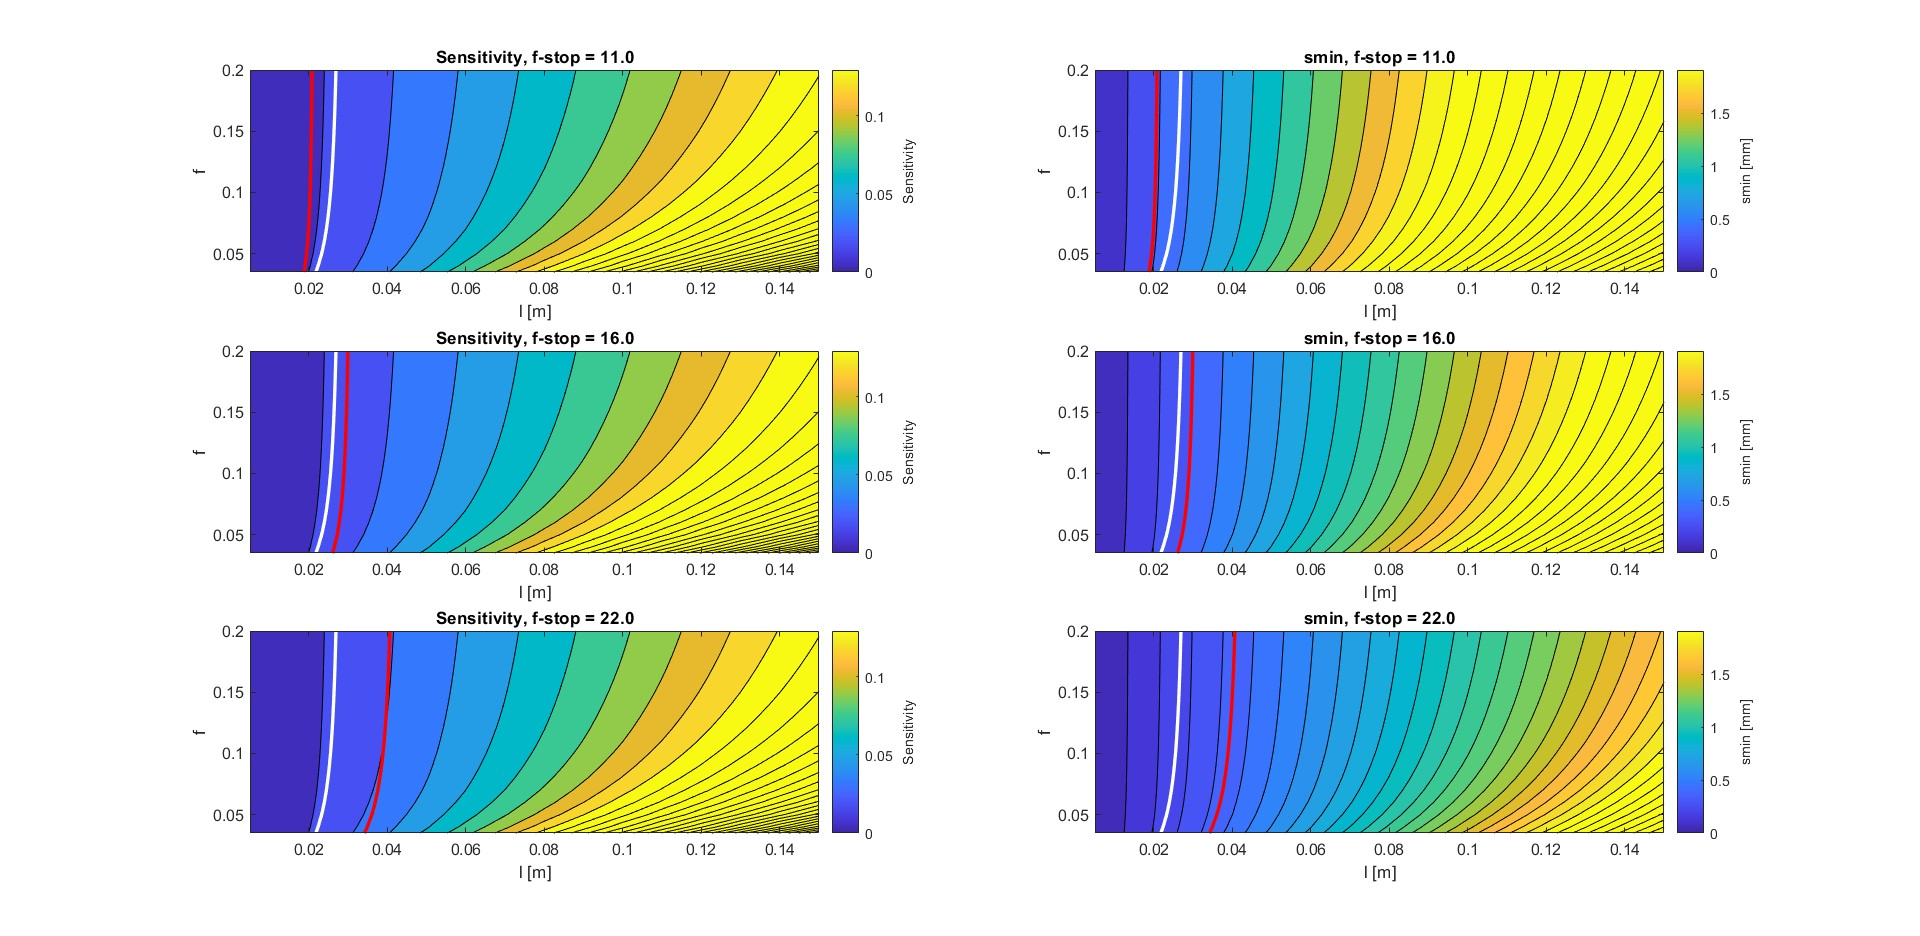
\includegraphics[width=1\textwidth]{figures/Sensitivity and dav SBOS surf map.jpg}
    \caption{Surface maps of $S$ and $s_{min}$ for $f_\# \in $ [11,16,22],  $f \in $ (0.035,0.200) and $l \in$ (0.005,0.15) for a negative defocus setup, with the red isoline representing the points where $s_{min}$ =0.0004 m and the white line showing $S=0.02$.}
    \label{fig: S and dav design surfmap SBOS}
\end{figure}

\par From Figure \ref{fig: S and dav design surfmap SBOS}, it is possible to draw the main trends in the two performance parameters, Sensitivity and $s_{min}$, with changing focal length $f$ and defocus distance $l$. The sensitivity seems to improve with a higher $l$, whereas the spatial resolution is worsened, signaled by an increase in the smallest distinguishable feature size $s_{min}$. For a fixed $l$, both $S$ and $s_{min}$ increase with lower $f$ but the effect becomes less prominent for higher focal length values. This means that a shorter focal length can reach the same sensitivity as a longer one at a smaller $l$, at the cost of a proportionally larger $s_{min}$. Moreover, the larger isoline gaps present at higher $f$ means that the system performance is less prone to changes for small deviations in $l$, which makes it more robust to uncertainties and errors induced during the setup assembly. This means that a higher $f$ and a lower $l$ are desirable for an optimal optical setup.

\par The figure also shows that the f-stop number can be used to easily increase the setup performance, as previously mentioned. When comparing the trends in sensitivity and $s_{min}$ for the 3 different $f_\#$, the red isoline moves more to the right than the white isoline when the f-stop increases. From this, it follows that a higher f-stop allows for better spatial resolution while still maintaining high sensitivity. From equations \ref{equation: df}, \ref{equation: Thin Lens equation}, \ref{equation: M} and \ref{equation: LFoVobj BOS}, it can be seen that $M$, $m$ and $d_f$ are independent of $f_\#$. This means that a change in $f_\#$ can be made by only changing it in the camera lens while maintaining the same optical setup. Consequently, the f-stop should ideally be set to the highest possible to optimize the sensitivity-resolution trade-off.

\par Other important parameters to analyze are the optical magnification $M$ and the distances $m$ and $d_f$, defined in Figure \ref{fig: SBOS with negative l}. The magnification describes how amplified the image is related to the real object and, as previously determined, it influences the sensitivity-resolution. The distances define how close the test section and in-focus plane are from the camera and directly influence $M$, which makes them important practical parameters that define the setup size. Figure \ref{fig: M,m and df design surfmap SBOS} presents the surface maps of these quantities for a given range of P.

\begin{figure}[htbp]
    \centering
    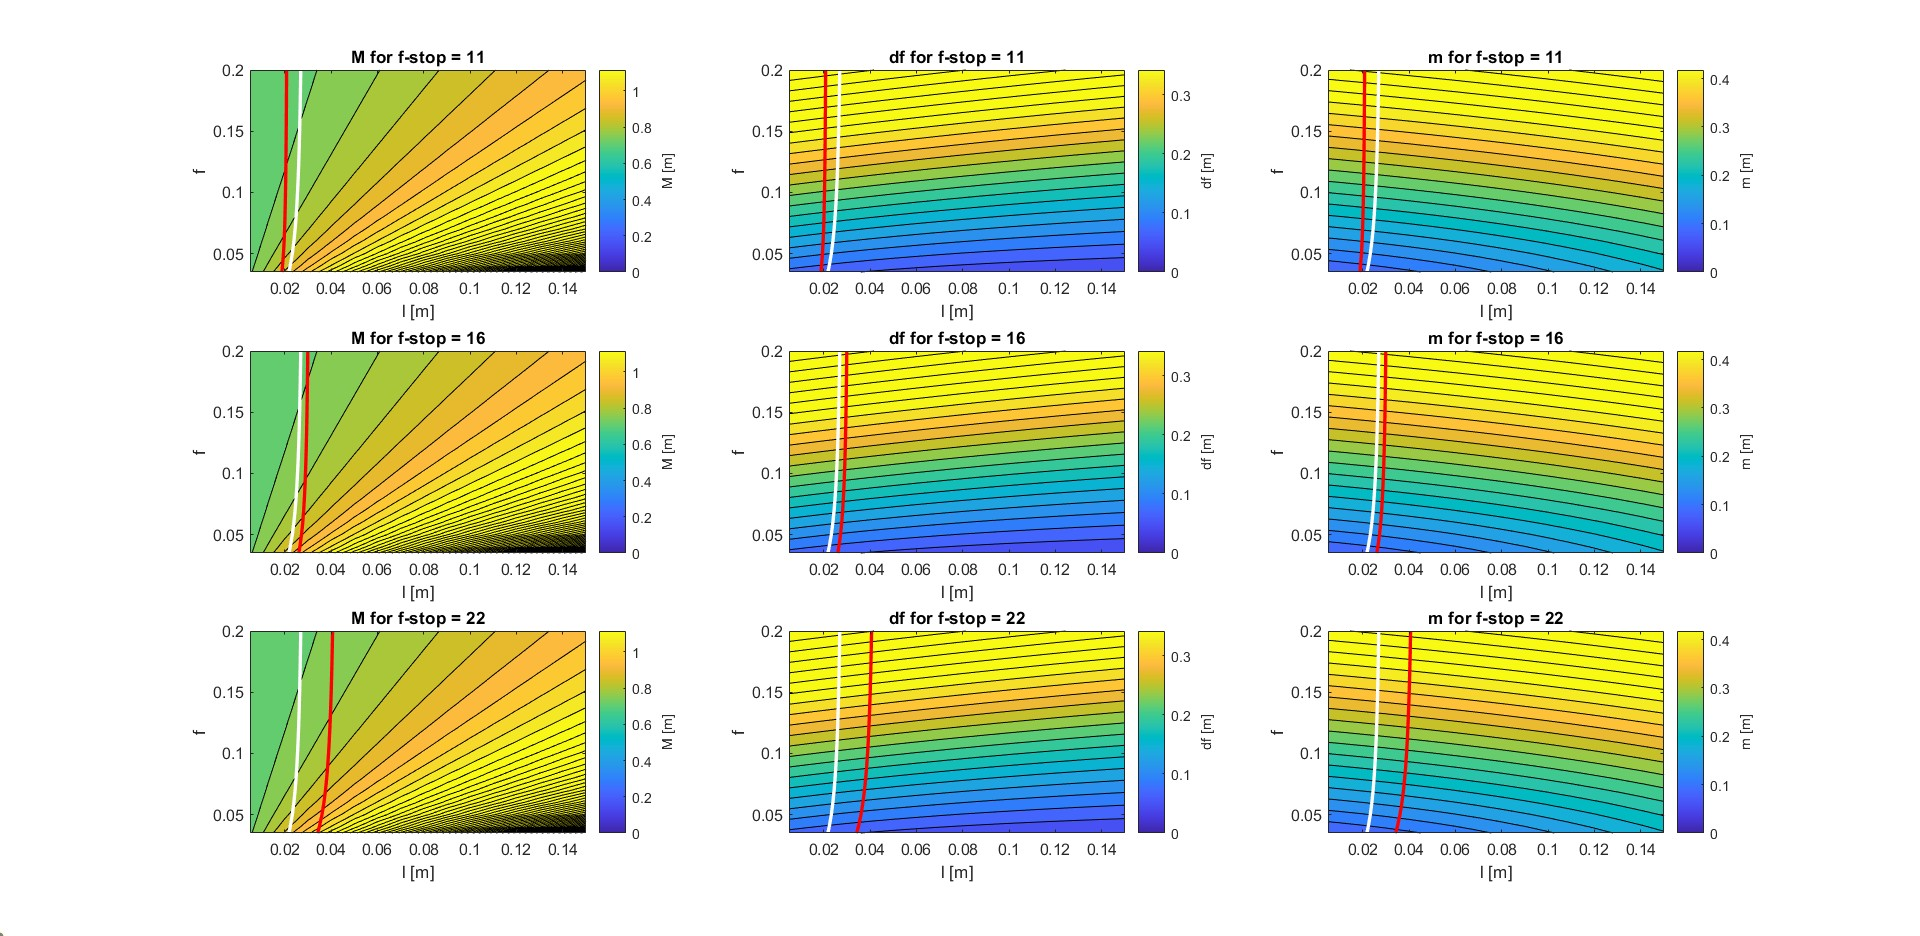
\includegraphics[width=1\textwidth]{figures/M,m,df surfmaps SBOS.jpg}
    \caption{Surface maps of $M$, $m$ and $d_f$ for $f_\# \in $ [11,16,22],  $f \in $ (0.035,0.200), $l \in$ (0.005,0.15) and $L_{FoV_{obj}}=$ 2cm of a negative defocus setup, with the red isoline representing the points where $s_{min}$ =0.0004 m and the white line showing $S=0.02$.}
    \label{fig: M,m and df design surfmap SBOS}
\end{figure}

From Figure \ref{fig: M,m and df design surfmap SBOS}, the distance $m$ only increases slightly along $l$ but presents a steep gradient in the $f$ axis. Together with the findings of Figure \ref{fig: S and dav design surfmap SBOS}, where $S$ and $s_{min}$ don't vary much with $f$, this suggests that a smaller focal length lens could be used to obtain a more compact setup with little cost in sensitivity and spatial resolution. Recall that the gradients of $S$ and $s_{min}$ in relation to $f$ become more intense with lower $f$. Consequently, a moderate focal length such as $f = 0.1$ m is preferable to a considerably shorter one such as $f = 0.05$ m, where the gradients of $S$ and $s_{min}$ are steepest. It can also be argued in favor of $f = 0.1$ m over a longer lens such as $f = 0.2$ m, given the savings in space. Nonetheless, the recommendations made for $f$ earlier in this section still hold, meaning that if the dimension of the setup is not a constraint, a higher $f$ is more desirable.

%\par The Figure also shows the trends on optical magnification. The surface maps show that $M$ increases with higher defocus distance, whereas it tends to decrease with higher$f$. It is true that a higher magnification allows the image to have more pixels per millimeter in the in-focus plane but if the object field of view is fixed, the pixel density in the object plane is also constant. Consequently the ability to capture details of the object is limited to how much blur is present. Figure \ref{fig: S and dav design surfmap SBOS} shows that a smaller $f_\#$ will lead to a blurrier image, so it is possible that a higher magnification won't help increase the resolution. A higher magnification also makes the captured image more prone to errors due to vibrations on the setup. Therefore, a trade-off must be done, where the level of blur is balanced such that the setup resources can be used efficiently. %This paragraph is confusing, I should REVISE it

\par The Figure also shows the trends on optical magnification. The surface maps show that $M$ increases with higher defocus distance, whereas it tends to decrease with higher $f$. The optical magnification can be accurately measured via a calibration plate in the in-focus plane, therefore it will be an important parameter to be validated during the experiment. Moreover, equation \ref{equation: S over smin} shows that the sensitivity-resolution ratio grows monotonically with $M$. 

\par As discussed in chapter \ref{chapter: LiteratureReview}, the minimum speckle size is also an important parameter as it limits the spatial resolution by restricting the allowable interrogation window size on the cross-correlation software. Figure \ref{fig: Delta s design surfmap SBOS} shows how the speckle size changes for a given range of P. Since $\Delta s$ is directly dependent on the magnification through equation \ref{equation: Rayleigh Limit}, it has the same trends as $M$. However, the f-stop number has a much bigger effect in $\Delta s$. It is recommended in the literature to limit the speckle size to 2-5 pixels to ensure optimal cross-correlation and avoid peak locking errors \cite{KahlerEtAl}, which essentially also limits the usable f-stop numbers of the setup. In this studied case, this means that $f_\#$ shouldn't be bigger than 22 nor smaller than 11.

\begin{figure}[htbp]
    \centering
    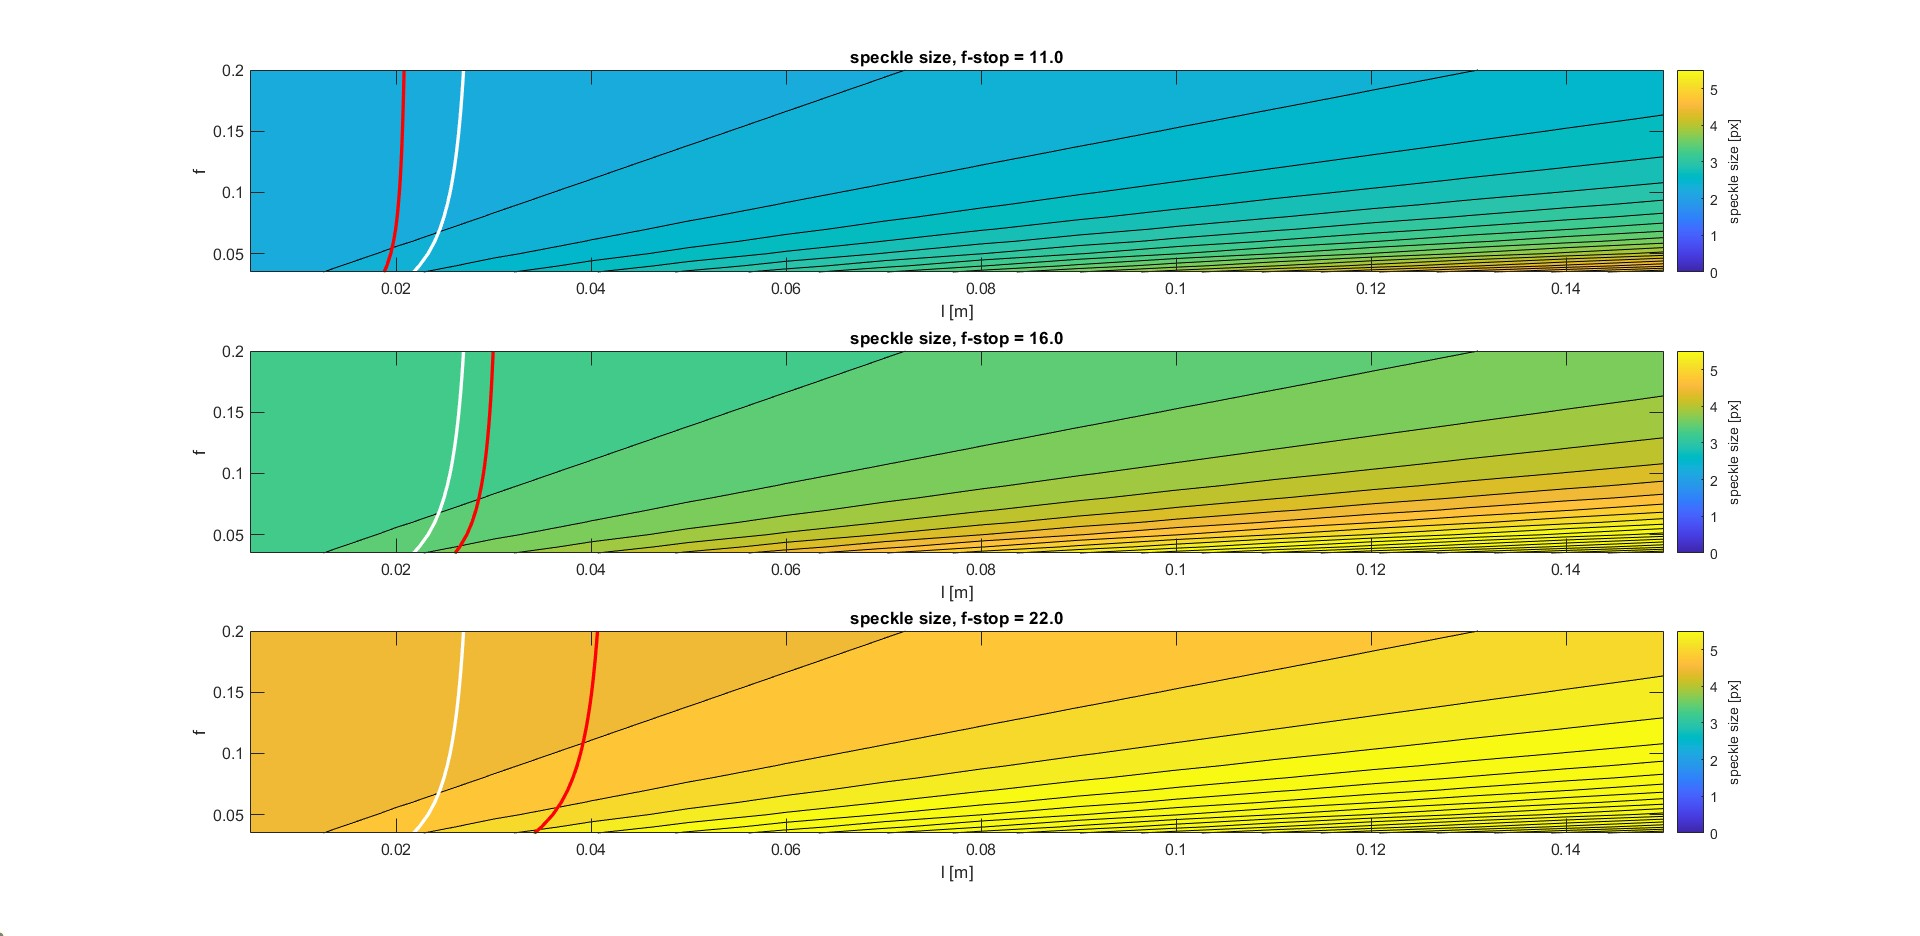
\includegraphics[width=1\textwidth]{figures/Speckle size surf map SBOS.jpg}
    \caption{Surface maps of $\Delta s$ for $f_\# \in $ [11,16,22],  $f \in $ (0.035,0.200), $l \in$ (0.005,0.15) and $L_{FoV_{obj}}=$ 2cm for a negative defocus setup, with the red isoline representing the points where $s_{min}$ =0.0004 m and the white line showing $S=0.02$.}
    \label{fig: Delta s design surfmap SBOS}
\end{figure}

\par It must be said that the speckle generation process is random at its heart \cite{Cloud2007}. The minimum speckle size is defined by the Rayleigh criterion but the average dimension might be bigger than the expected. If it happens that the average speckle size is bigger than 5 pixels, the downside will be the need to use larger interrogation windows, therefore reducing the spatial resolution. Nevertheless, if a high magnification is being used, a big interrogation window might still lead to a small vector pitch and an acceptable resolution. Therefore, there is more to the spatial resolution than the amount of blur in the image as it can also be affected by the CC post-processing. This amounts to the question: how is it possible to reconcile both resolutions such that no resource is being wasted to get a better optical resolution and obtaining a worse processing resolution? Section \ref{section: SR criteria} answers this question and provides a design criterion to choose the best BOS setup. Before getting into the SR criterion, it is worth first analysing how negative defocus compares with positive defocus in the next section.
 
\subsection{Surface Maps for positive defocus setup}
\label{subsection: Surface maps for BOS}

\par Surface maps for a standard BOS setup were also obtained. These maps allow for a comparison of the trends permeating the design space of a positive defocus to the negative defocus present in the last section. Similarly to subsection \ref{subsection: Surface Maps for SBOS}, this subsection will show and discuss the main trends in sensitivity, spatial resolution, $M, m, d_f$ and speckle size $\Delta s$, given $L_{FoV_{obj}}=$ 2cm, $\lambda = 632.8$nm, pixel size equal 6.5 $\mu$m, sensor dimension of 2560x2160 pixels, resulting in $L_{sens}$ = 1.4cm. Figure \ref{fig: S and smin surfmap BOS} contains surface maps of Sensitivity and $s_{min}$ given a range of P.

\begin{figure}[htbp]
    \centering
    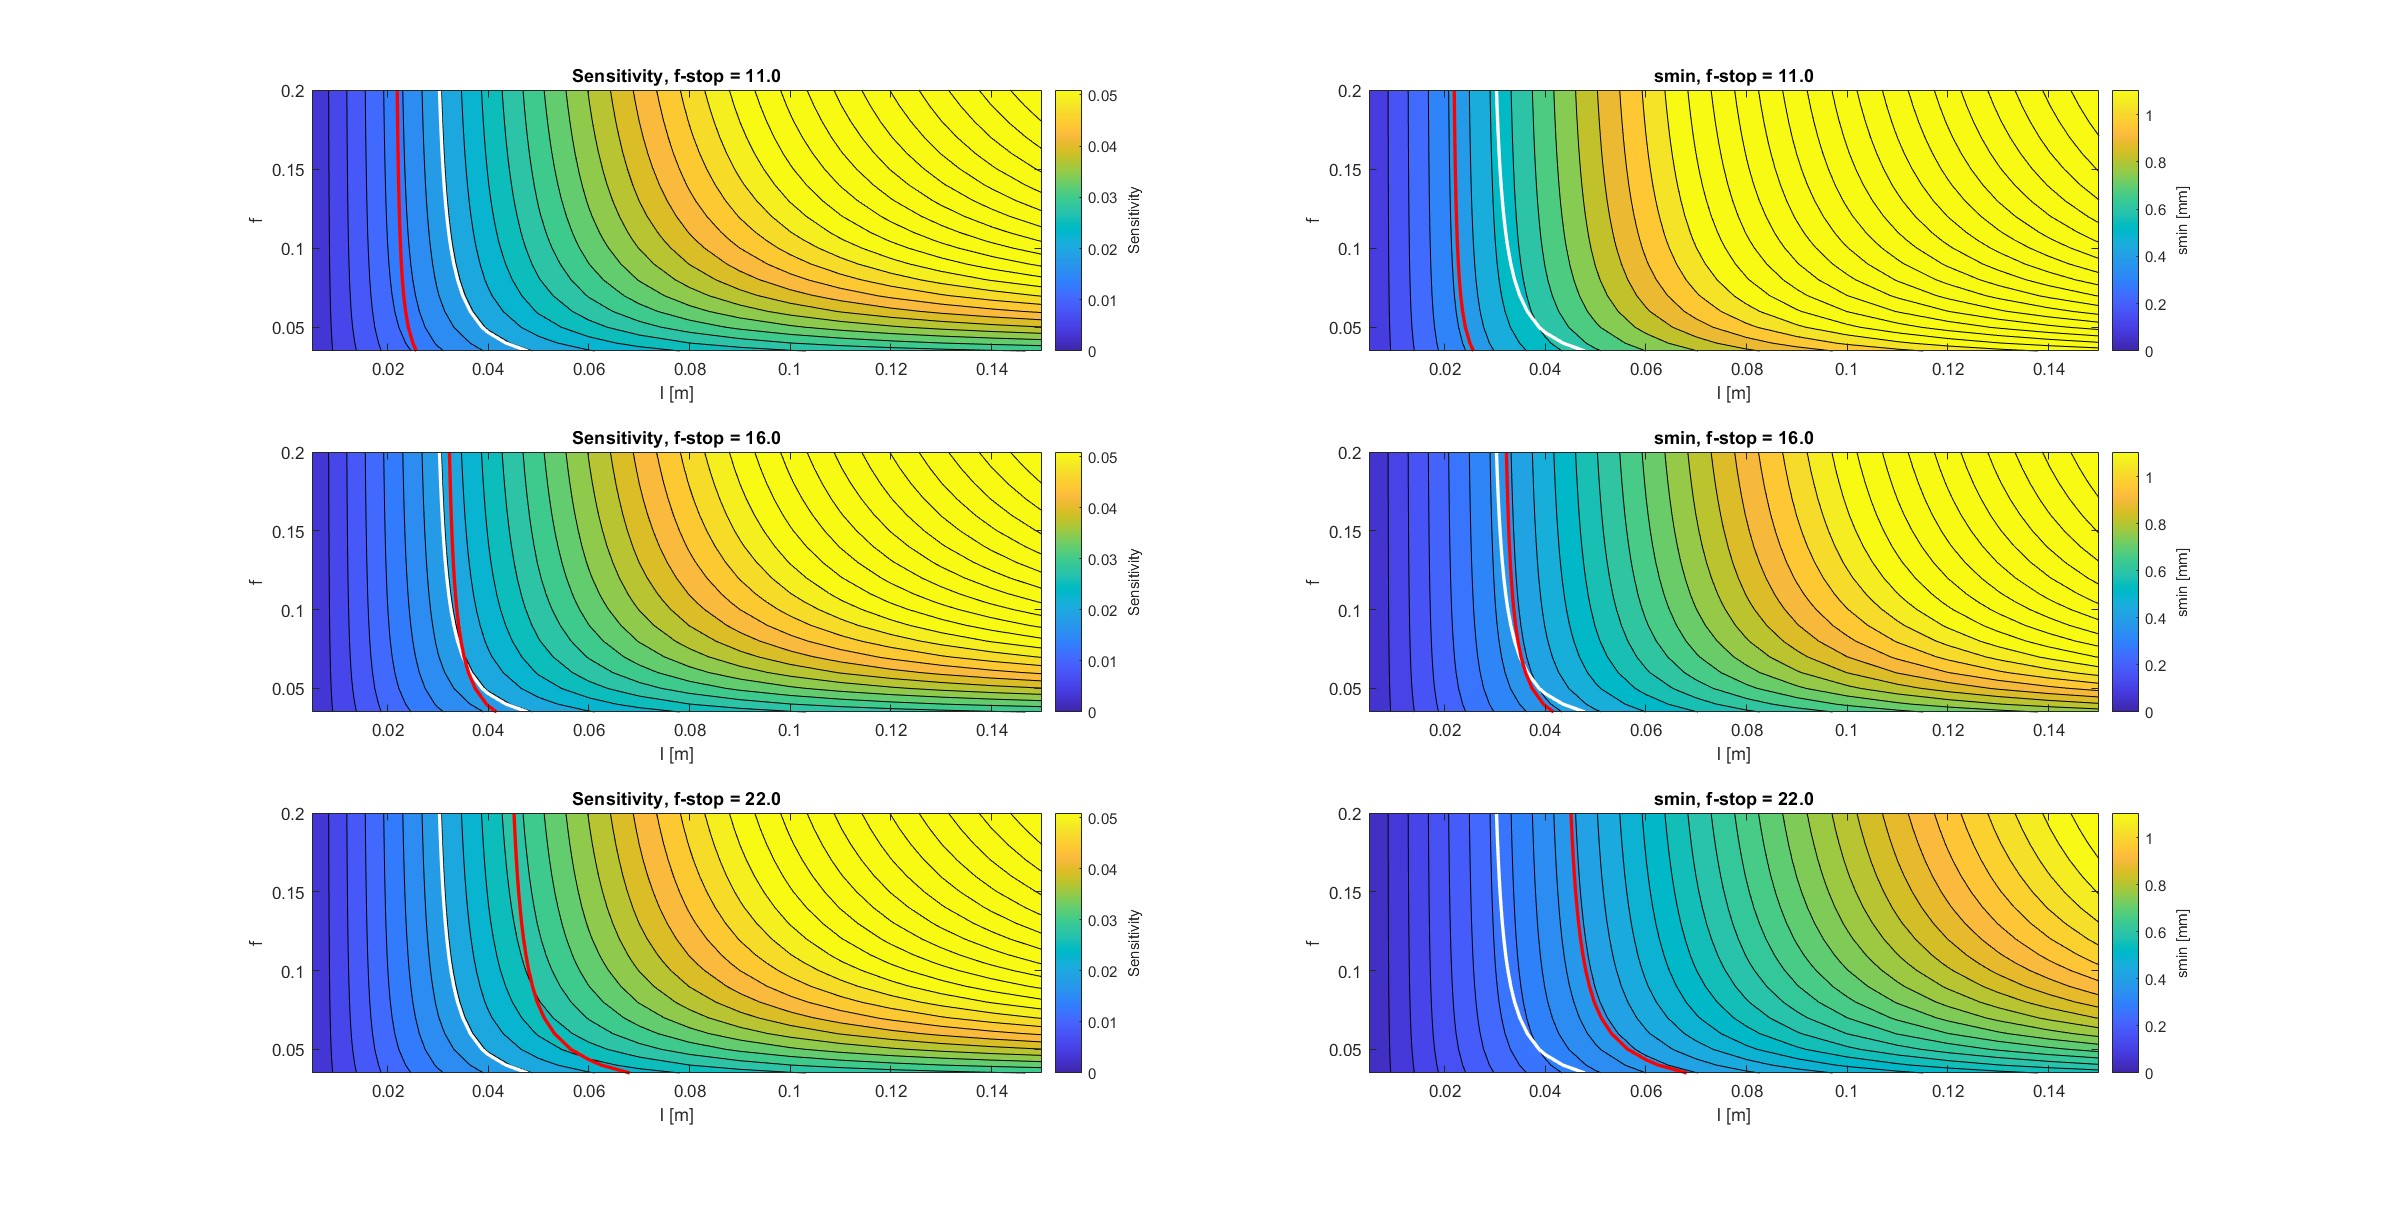
\includegraphics[width=1\textwidth]{figures/Sensitivity and smin BOS surf map.jpg}
    \caption{Surface maps of $S$ and $s_{min}$ for $f_\# \in $ [11,16,22],  $f \in $ (0.035,0.200), $l \in$ (0.005,0.15) and $L_{FoV_{obj}}=$ 2cm of a positive defocus setup, with the red isoline representing the points where $s_{min}$ =0.0004 m and the white line showing $S=0.02$.}
    \label{fig: S and smin surfmap BOS}
\end{figure}

\par Through Figure \ref{fig: S and smin surfmap BOS}, the main trends on sensitivity and spatial resolution for a positive defocus setup can be analyzed. Both parameters seem to reach an asymptote for higher $l$. The higher the $f$, the higher the asymptote value. Moreover, it seems that the sensitivity is unaffected by $f_\#$, while the $s_{min}$ asymptotes moves up and right for an increasing f-stop, meaning that a higher f-stop allows for a better spatial resolution for the same sensitivity, as demonstrated by equation \ref{equation: S over smin}. Recall the discussion from section \ref{section: Background Oriented Schlieren} where a fundamental limit of the sensitivity was obtained by taking the limit for $l \to \infty$. This means that the sensitivity asymptotes shown in Figure \ref{fig: S and smin surfmap BOS} will lead to $S$ converging to $f$, which is summarized in equation \ref{equation: BOS Sensitivity limit}. Consequently, no matter how far away the background is positioned in a positive defocus configuration, the sensitivity will ultimately be limited by the focal length of the camera, whereas with the negative defocus, sensitivity is unbounded. Nevertheless, while designing the setup, the same recommendation reached for SBOS also applies for BOS, a higher focal length and f-stop is the most desirable.

\begin{equation}
    \label{equation: BOS Sensitivity limit}
    \lim_{l \to \infty}S = f
\end{equation}

Regarding $M,m$ and $d_f$, Figure \ref{fig: M,m and df design surfmap BOS} shows that the positive defocus setup variables have different trends compared to a negative one. Variables $m$ and $d_f$ seem to have switched behaviors if compared to their trends in section \ref{subsection: Surface Maps for SBOS}, with $m$ increasing slightly with $l$, while $d_f$ decreases little with $l$, and both increasing considerably with $f$. Due to the large gradient of both distances in the $f$ axis and the nature of the $S$ and $s_{min}$, similarly to the negative defocus case, it is possible to obtain a more compact setup using a smaller focal length if needed, with little loss in sensitivity and spatial resolution. Comparing $M$ from positive $l$ to negative $l$, it is worth noting that the absolute values are smaller and the trend is inverted, which strengthens the argument that SBOS presents a higher $S$ for the same $s_{min}$ due to an increase in $M$. The decrease in $M$ also reflects in a smaller speckle size for the BOS case through equation \ref{equation: Rayleigh Limit}, this can be seen in Appendix \ref{Appendix: Speckle size BOS map}.

\begin{figure}[htbp]
    \centering
    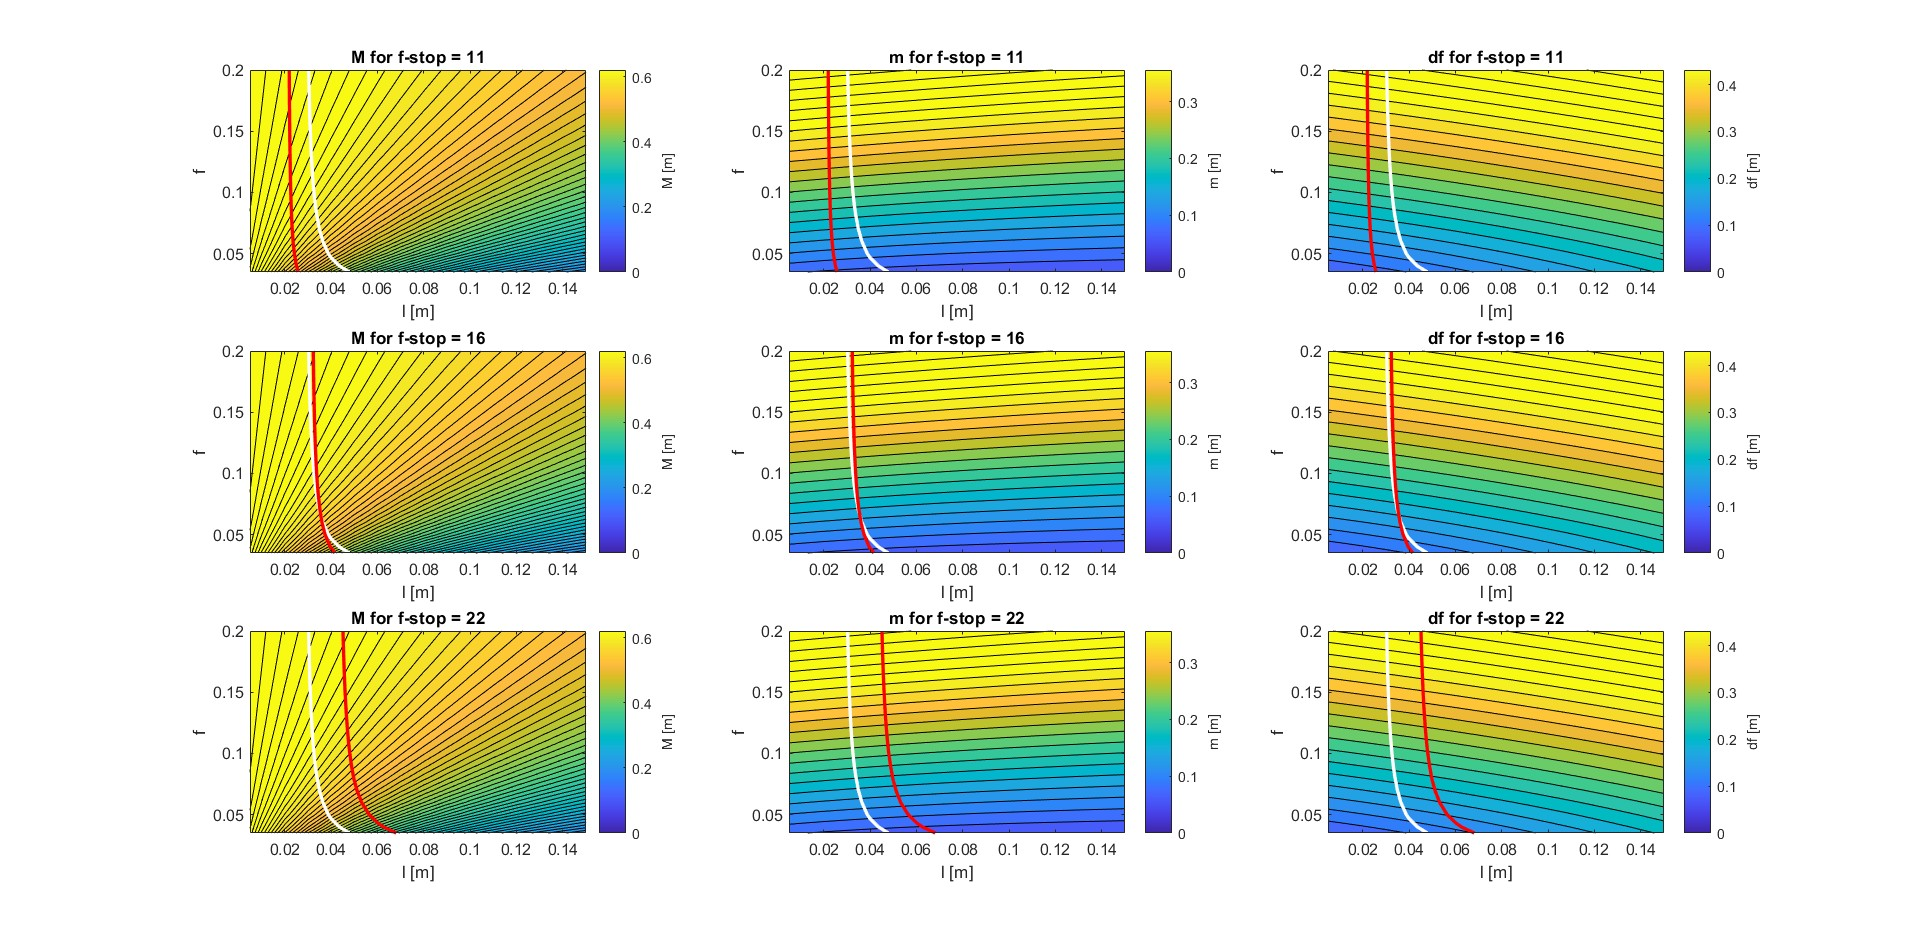
\includegraphics[width=1\textwidth]{figures/M,m,df surfmaps BOS.jpg}
    \caption{Surface maps of $M$, $m$ and $d_f$ for $f_\# \in $ [11,16,22],  $f \in $ (0.035,0.200), $l \in$ (0.005,0.15) and $L_{FoV_{obj}}=$ 2cm of a positive defocus setup, with the red isoline representing the points where $s_{min}$ =0.0004 m and the white line showing $S=0.02$.}
    \label{fig: M,m and df design surfmap BOS}
\end{figure}

\subsection{Effect of FoV}
\label{subsection: Effets of FoV}
\par Since the final goal of this thesis is to implement the SBOS method to a wind-tunnel application, it is also worth investigating the effect of altering the size of the field of view. Surface maps will be used to compare the trends in sensitivity and spatial resolution of negative and positive defocus setups when the $L_{FoV_{obj}}$ is changed from 2cm to 7cm. Figure \ref{fig: Surface maps altering FoV} shows these graphs, surface maps for other parameters can be found in Appendix \ref{Appendix: FoV 70mm maps}. For this case, the red isoline value has been slightly modified to $s_{min}$ =0.00035 m. However it still allows the comparison with previous images given the very small difference between them.

\begin{figure}[htbp]
  \centering
  \begin{subfigure}{0.9\textwidth}
    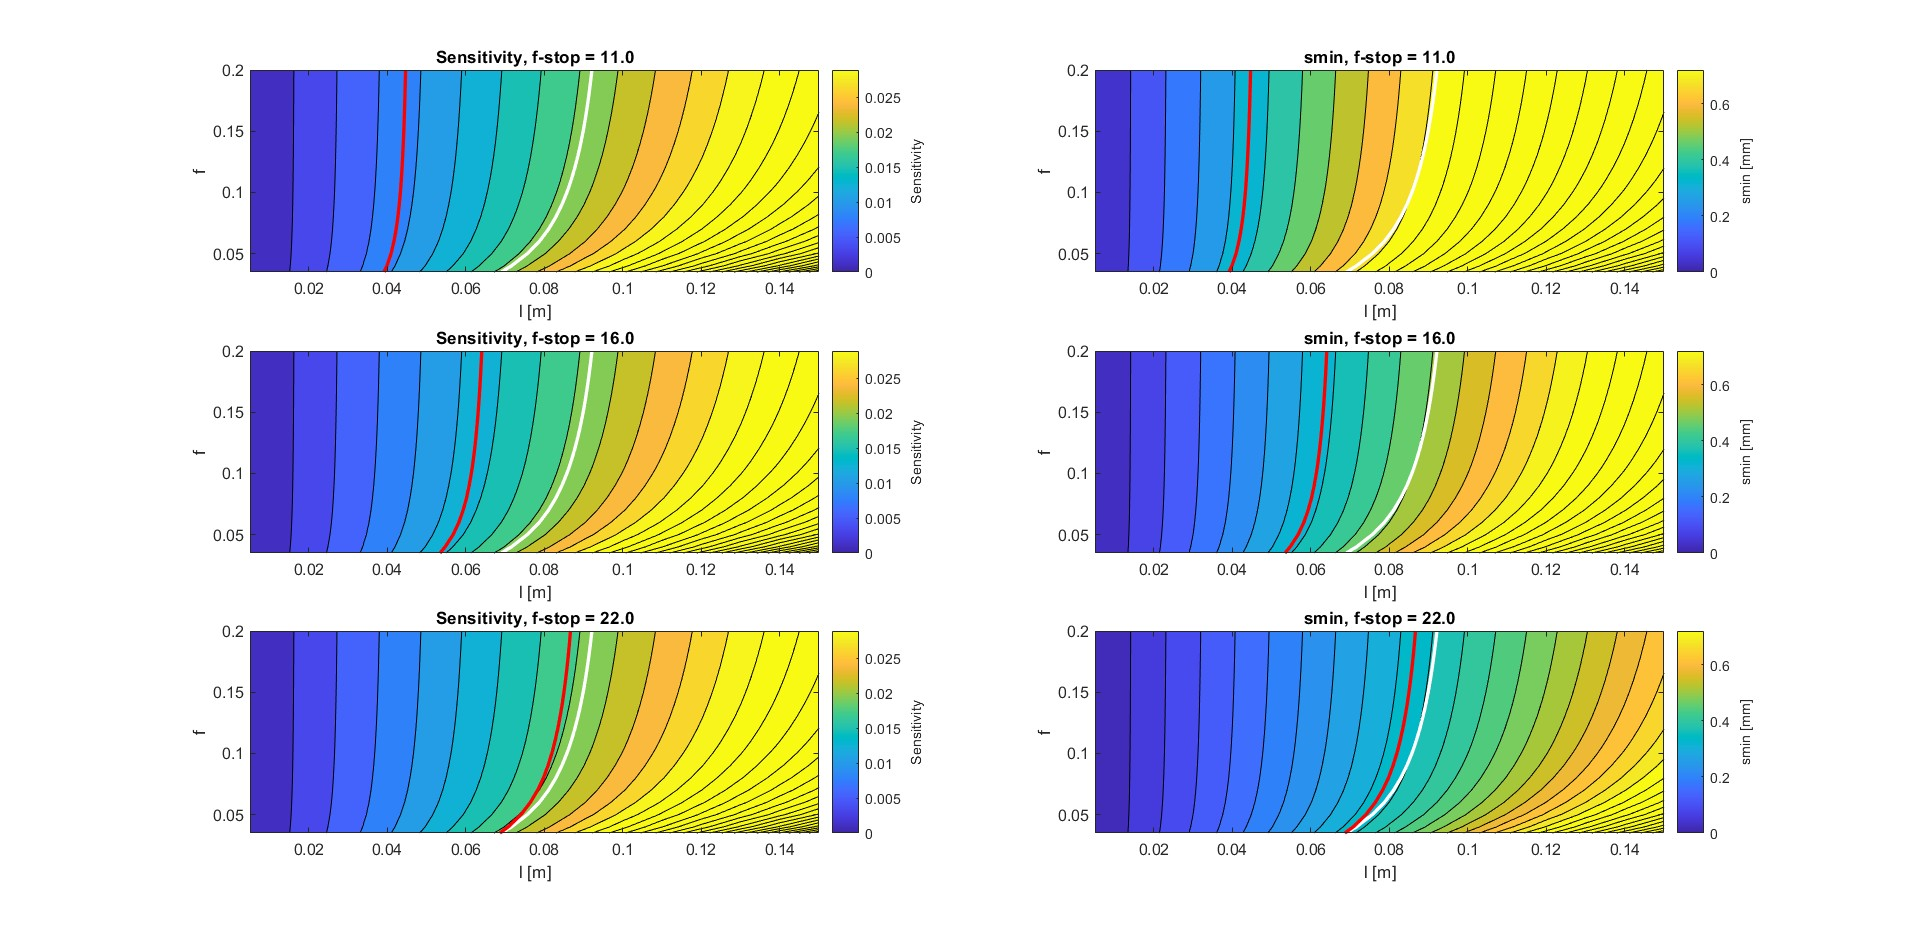
\includegraphics[width=\textwidth]{figures/Sensitivity and smin SBOS surf map 70cm.jpg}
    \caption{}
  \end{subfigure}
  \hfill
  \begin{subfigure}{0.9\textwidth}
    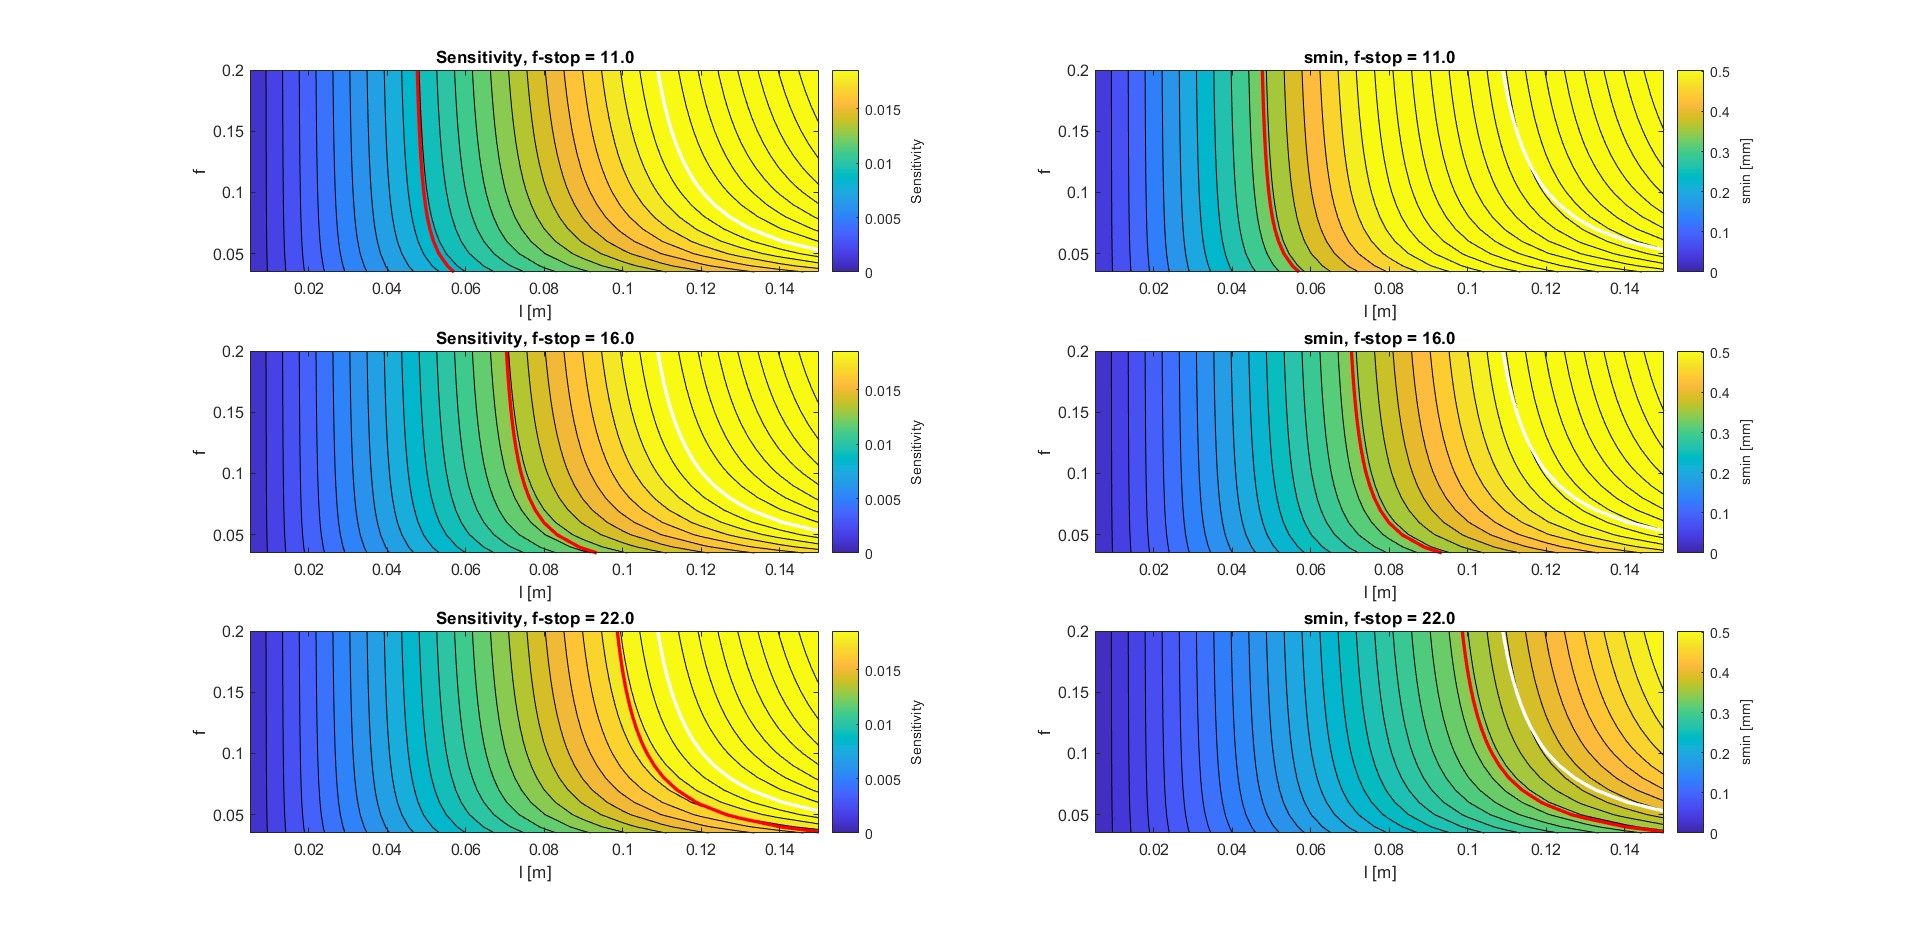
\includegraphics[width=\textwidth]{figures/Sensitivity and smin BOS surf map 70mm.jpg}
    \caption{}
  \end{subfigure}
  \caption{Surface maps of $S$ and $s_{min}$ for $f_\# \in $ [11,16,22],  $f \in $ (0.035,0.200), $l \in$ (0.005,0.15) and $L_{FoV_{obj}}=$ 7cm of a negative defocus setup (a) and a positive defocus setup (b), with the red isoline representing the points where $s_{min}$ =0.00035 m and the white line showing $S=0.02$.}
  \label{fig: Surface maps altering FoV}
\end{figure}

\par From Figure \ref{fig: Surface maps altering FoV} some differences from the surface maps presented at subsections \ref{subsection: Surface Maps for SBOS} and \ref{subsection: Surface maps for BOS} can be highlighted. Generally, a higher field of view results in smaller $S$ and $s_{min}$ due to the smaller optical magnifications needed to achieve the desirable window size, as per equation \ref{equation: M} and \ref{equation: S over smin}. This results in a much higher defocus distance needed to achieve the same $S$. It also translates in less susceptibility to obtain blurred images, which is signaled by the generally smaller $s_{min}$. This is evident from the position of the red and white isolines, which are both located at much higher $l$'s than their smaller $L_{FoV_{obj}}$ counterparts. This characteristic makes the advantage of SBOS even more prominent: with negative defocus a higher sensitivity can be achieved at lower $l$'s while maintaining a low $s_{min}$.

\par Up until now, the surface maps have been useful to visualize the equations displayed in section \ref{section: Geometries of a SBOS optical setup}, \ref{section: Sensitivity-Resolution Ratio} and understand better the trends that exist between variables. However, a definitive criterion to choose the best optical setup is still missing. This will be done by solving a problem mentioned in subsection \ref{subsection: Surface maps for BOS}, to match the optical spatial resolution and software spatial resolution so the experimenter can more efficiently use the its resources. The solution is presented in the next section.

\section{SR criterion}
\label{section: SR criteria}

To reconcile the optical spatial resolution and the post-processing resolution, it must be expressed in terms of pixels. Historically, $M$ has been used by researchers to provide an insight on how much detail the camera can capture, as it defines the pixel density through equation \ref{equation: Px density} \cite{Schmidt2025, Gojani&Obayashi}. However, since the object is blurred, it is not necessarily true that a higher pixel density will lead to a better spatial resolution as the number of pixels per millimeter may increase together with the size of the blur, as per equation \ref{equation: CoC BOS}. 

\par Moreover, given that the object is out of focus, its size differs from the one it would have if it were in focus (see appendix \ref{Appendix: Blurred Object}). Therefore, there are two magnifications at play in the setup, one for the blurred object and another for the in-focus plane. The blurred object magnification is fixed by the desired field of view and camera, defined by equation \ref{equation: M obj}. Whereas the optical magnification shown in Figure \ref{fig: M,m and df design surfmap SBOS} is defined by equation \ref{equation: M}. The amount of detail truly captured by the camera is constrained by $M_{obj}$, fixed by the defined object field of view. It also defines how many pixels can image a mm of the object, through the pixel density (equation \ref{equation: Px density}) and influences the blur of the image, via equation \ref{equation: smin}. Consequently, a trade-off must be done, where the level of blur is balanced with the pixel density such that the setup resources can be used efficiently.

\begin{equation}
    \label{equation: Px density}
    Px_{density} = \frac{M}{Px_{Size}},
    \qquad
    Px_{density_{obj}} = \frac{M_{obj}}{Px_{Size}}
\end{equation}

One way to make this trade-off is to express $s_{min}$ in pixels via Eq. \ref{equation: smin px}, which combines the pixel density with the spatial blur. Dividing the sensor dimension by this quantity gives the ratio $SR$ (Eq. \ref{equation: SR}), which is equivalent to $L_{FoV_{obj}}/s_{min}$ and therefore represents the number of resolvable features across the object field of view. Specifying $SR$ thus fixes how finely the flow is sampled, and with it the number of pixels available to image each feature. For example, $s_{min[px]} = 10$ px ($SR \approx 200$) could be selected: the feature is then spanned by 2–3 speckles and correlated with a 32 px interrogation window at 75\% overlap, giving a vector spacing of 8 px and ensuring the feature is resolved by the vector field.

\begin{equation}
    \label{equation: smin px}
    s_{min_{[px]}} = s_{min} \cdot Px_{density_{obj}}
\end{equation}

\begin{equation}
    \label{equation: SR}
    SR = \frac{L_{sens}}{s_{min_{[px]}} \cdot Px_{Size}}
\end{equation}

\par By defining $SR$, an isoline can be drawn in the surface maps where that condition is met. Together with the previous recommendations: select the highest $f$ for robustness, highest $f_\#$ to obtain the better $S/s_{min}$ trade-off, while keeping $\Delta s$ small enough; the physical distances $l$, $m$ and $d_f$ can be defined. This way, a design point can be selected that optimizes the performance parameters given the available resources.

\section{Summary of Practical Guidelines}
\label{section: Summary of Practical Guidelines}

\par Taken together, the geometric analysis of section \ref{section: Geometries of a SBOS optical setup}, the discussion of section \ref{section: Sensitivity-Resolution Ratio}, the design space exploration of section \ref{section: Design Strategy} and the SR design criterion of section \ref{section: SR criteria} establish a consistent set of guidelines for both BOS and SBOS setups: 

\begin{itemize}
    \item Higher focal length makes the SBOS system more robust to position errors and increases the sensitivity limit for BOS. If size is a constraint, a lower $f$ can result in a more compact setup
    \item A higher f-stop number is generally desirable, subject to the speckle-size constraint of 2–5 pixels
    \item Negative defocus configuration favors a lower defocus distance to exploit its inherent sensitivity advantage over standard BOS
    \item If $f$ and $f_\#$ are maximized, the $SR$ criterion can be used to select the setup that gives the best balance between the optical and CC spatial resolution
    \item SBOS allows for finer speckle sizes than printed BOS, making it possible to study smaller fields of view.
\end{itemize}

Taken together, these guidelines constitute the answer to the first research sub-question posed in Chapter \ref{chapter: introduction}, namely what the practical guidelines for the design of a SBOS setup should be when balancing the trade-off between sensitivity and spatial resolution. They were used to select the design point of the first experimental campaign, balancing sensitivity and spatial resolution. The following chapter describes the resulting experimental setups, built as a proof of concept to validate this design strategy before the method is applied to the more demanding wind tunnel environment. 

\chapter{Experimental Setups}
\label{chapter: Experimental Setups}

\par A small experimental setup using a simple object as a case study was built to prove the presented concepts and validate the design strategy. Moreover, this "proof of concept" experimental campaign was used to compare multiple optical configurations, assess their performance and investigate the underlying uncertainty sources. Later, a second experiment was conducted to improve the speckle pattern quality and image a compressible jet. All the information gathered was then applied to the visualization of the flow through an aerospike nozzle in a supersonic wind tunnel. The description of each setup follows below.

\par Each campaign is described by the same structure: the objective and the research question it addresses, the object of study, the optical layout and hardware, definition of the design points, the acquisition and processing settings, the sources of uncertainty specific to that setup, and the test matrix.


\section{Angled Glass Experiments}
\label{section: Angled Glass Experiment}

\par The first experimental campaign was envisioned to validate the surface maps presented in the last section and effectively compare a negative and positive defocus configuration in terms of its performance parameters for a similar object field of view. In order to achieve that, an experimental setup was built  where the optical distances could be easily set and modified. The setup was assembled on an optical rail close to the ground to avoid vibrations and followed the same structure as the schematic shown in Figure \ref{fig: SBOS with negative l}. 

\par Regarding hardware, Figure \ref{fig: Angled glass setup} shows the assembled setup. The laser used was a LIMAB model RC 0.5, a class 2 continuous red light laser ($\lambda = 632.8$ nm) with 0.5 mW of power. Given the class of the laser, safety was inherently guaranteed against accidental exposure, as the risk of eye injury is limited by the blink reflex. Nevertheless, simple procedures were made to make sure that the laser paths were contained and terminated. To diffuse the laser and create the speckle pattern, a small ground glass was used with only 1.27 cm of diameter. As it can be seen in the picture, the ground glass was positioned close to laser collimator, which was adjusted to fill the whole diameter of the ground glass. To image the displacements, LaVision's Imager sCMOS CLHS was used, it has a pixel size of 6.5 \si{\micro \meter} and a sensor dimension of $2560 \times 2160$ pixels. The camera was equipped mainly with a 200 mm camera lens. Two images with a 105 mm lens were taken, however, it was quickly changed back to the 200mm one, as it provided a more stable and robust assembly.

\begin{figure}[h]
    \centering
    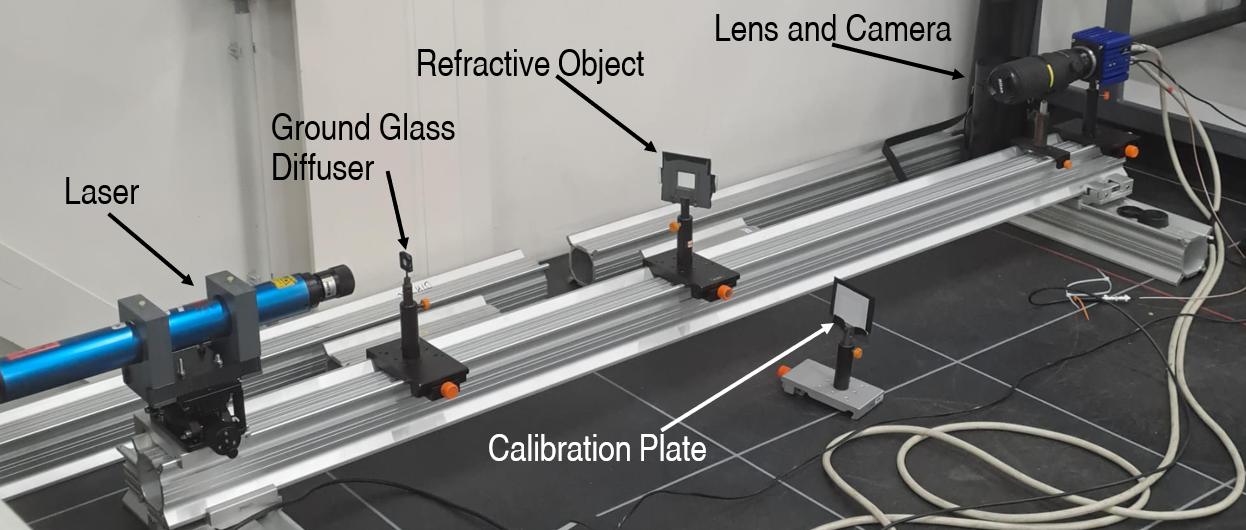
\includegraphics[width=\textwidth]{figures/small sbos setup with captions.png}
    \caption{Assembled setup of the angled glass campaign. The laser and the ground glass diffuser are mounted at the near end of the rail, the angled glass refractive object at mid-span and the lens and camera at the far end. The calibration plate, used to measure the optical magnification $M_{ag}$ in the in-focus plane, is shown on its own mount.}
    \label{fig: Angled glass setup}
\end{figure}



\par To simplify the experiment, a small angled piece of glass was used as refractive object, similar to what Schwarz \& Braukmann \cite{Schwarz&Braukmann} and Meier \& Rösgen \cite{Meier&Roesgen2013} have used. As shown in Figure \ref{fig: Angled glass geometry}, the angled glass introduces a uniform unidirectional displacement to the speckle background that can be predicted using Equation \ref{equation: Displacement of angled glass}. By dividing the displacement measured by the camera $\Delta x$ and the displacement induced by the refractive object $\varepsilon$, it is possible to obtain the setup sensitivity $S$, as shown in Equation \ref{equation: S BOS}. It is worth noting that the definition of $\varepsilon$ in this case is an artifice because the real displacement $\Delta x$ is independent of $l$. The $\varepsilon$ is used to connect a simple refractive object to a real experimental scenario. The glass piece used had a thickness $T = 2$ mm and a refractive index of around $n = 1.52 \pm 0.02$. 


 \begin{figure}[h]
   \centering
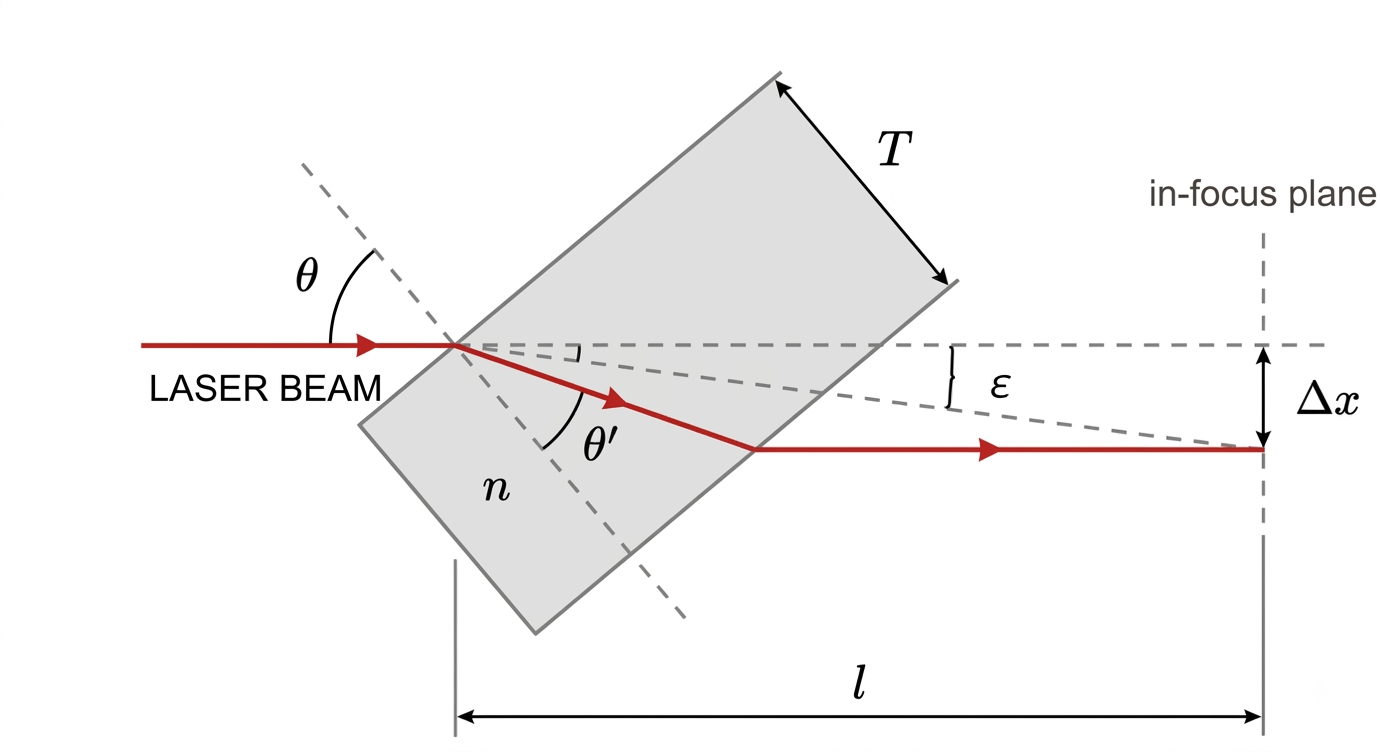
\includegraphics[width=0.7\textwidth]{figures/angled laser schematic.png}
    \caption{Geometry of the angled glass plate used as refractive object. A beam incident at an angle $\theta$ on a plate of thickness $T$ and refractive index $n$ is refracted to $\theta'$ and leaves the plate parallel to its original direction, laterally displaced by $\Delta x$. Over the defocus distance $l$ this displacement is equivalent to a uniform deflection angle $\varepsilon$.}
    \label{fig: Angled glass geometry}
\end{figure}

\begin{equation}
    \label{equation: Displacement of angled glass}
    \varepsilon = \frac{\Delta x}{l} =\frac{T}{l} \sin(\theta) \left( 1 - \frac{\cos(\theta)}{\sqrt{n^2-\sin^2(\theta)}}\right)
\end{equation}

\par Table \ref{tab: angled glass test matrix} shows the information of each point tested during the first campaign. The table lists not only the camera, lens configuration and optical distances, but also the theoretical magnification, sensitivity, predicted displacement given the measured glass angle and whether the in-focus plane was behind or in front of the refractive object. The points vary the type of configuration, the f-stop number, the defocus distance and the focal length of the camera and all of them have been obtained by computing the object field of view to be 2cm and inspecting the surface maps obtained with the code described in Chapter \ref{chapter: methodology}. In this instance then, the SR criterion has not been used, as the intention of the experiment was to validate the methodology by testing various different setups. Therefore, by comparing the theoretical sensitivity, magnification and the displacement with the ones obtained experimentally at each of these points, the methodology presented in Chapter \ref{chapter: methodology} can be validated. Moreover, through the comparison of experimental sensitivities obtained with a negative defocus against a positive defocus configuration, the difference in performance of SBOS versus BOS is obtained.

\begin{table}[h]
    \centering
    \caption{Optical configurations acquired during the angled glass campaign. $\theta$ is the angle at which the glass plate was set. ``Negative'' and ``Positive'' denote the in-focus plane lying respectively in front of or behind the test section, following the convention of Chapter \ref{chapter: methodology}. Points 1-9 correspond to the experiment with a similar $L_{FoV}$, whereas points 10-20 correspond to the linear slider experiment. In point 10 the refractive object is coincident with the in-focus plane, so no defocus type is defined.}
    \label{tab: angled glass test matrix}
    \begin{tabular}{lrrrrrrrl}
        \toprule
        Point & $f_\#$ & $f$ & $l$ & $d_f$ & $M_{ag}$ & $S$ & $\theta$  & Type of Defocus \\
              &         & [mm] & [mm] & [mm] & [--] & [mm] & [$^{\circ}$] & \\
        \midrule
        1    & 16 & 200 &  80 & 409.0 & 0.956 &  76.50 & 17 & Negative \\
        2    & 16 & 200 &  80 & 505.0 & 0.656 &  52.50 & 17  & Positive \\
        3    & 16 & 200 & 100 & 391.0 & 1.050 & 105.00 & 17  & Negative \\
        4    & 16 & 200 & 100 & 511.0 & 0.643 &  64.30 & 17  & Positive \\
        5   & 11 & 200 &  80 & 393.0 & 1.037 &  83.00 & 17  & Negative \\
        6   & 11 & 200 &  80 & 490.0 & 0.690 &  55.20 & 17  & Positive \\
        7   & 11 & 105 &  80 & 189.0 & 1.250 & 100.00 & 20  & Negative \\
        8   &  4 & 105 &  80 & 285.0 & 0.583 &  46.60 & 20  & Positive \\
        9   & 16 & 200 & 150 & 527.0 & 0.611 &  91.60 & 20  & Positive \\
        \midrule
        10 & 8 & 200 &  0 & 470.0 & 0.741 &  0.00 & 20    & --       \\
        11 & 8 & 200 & 10 & 470.0 & 0.741 &  7.41 & 20 & Positive \\
        12 & 8 & 200 & 20 & 470.0 & 0.741 & 14.81 & 20  & Positive \\
        13 & 8 & 200 & 30 & 470.0 & 0.741 & 22.22 & 20  & Positive \\
        14 & 8 & 200 & 40 & 470.0 & 0.741 & 29.63 & 20  & Positive \\
        15 & 8 & 200 & 50 & 470.0 & 0.741 & 37.04 & 20  & Positive \\
        16 & 8 & 200 & 10 & 470.0 & 0.741 &  7.41 & 20  & Negative \\
        17 & 8 & 200 & 20 & 470.0 & 0.741 & 14.81 & 20  & Negative \\
        18 & 8 & 200 & 30 & 470.0 & 0.741 & 22.22 & 20  & Negative \\
        19 & 8 & 200 & 40 & 470.0 & 0.741 & 29.63 & 20 & Negative \\
        20 & 8 & 200 & 50 & 470.0 & 0.741 & 37.04 & 20 & Negative \\
        \bottomrule
    \end{tabular}
\end{table}

Points 10-20 of Table \ref{tab: angled glass test matrix} describe the optical arrangement of a different configuration to the previous points. The setup presented in Figure \ref{fig: Angled glass setup} was modified to run an experiment intended to demonstrate the SBOS capacity of achieving different defocus configurations. The experiment consisted in keeping the in-focus plane fixed and moving the refractive object in steps with a linear slider, shown in Figure \ref{fig: Angled Glass Slider}. This kept the optical magnification constant, while permitting the exploration of a range of defocusing distances. Therefore the experiment can establish whether the advantage of the negative defocus configuration in achieving a higher sensitivity comes only from $M_{ag}$, or also from some other mechanism related to $l$.

The data acquisition followed standard BOS procedure using LaVision's DaVis 8.4 software. First, a calibration plate was used to define the in-focus plane, it can be seen in Figure \ref{fig: Angled glass setup}. From the calibration, DaVis computed the magnification and the pixel density of the setup. Then, the laser is turned on and a reference image is taken. The laser is turned back off and the refractive object is put into position following the distances presented in the surface maps of Chapter \ref{chapter: methodology}. With the laser back on, a displaced image is taken. Post-processing was done using LaVision DaVis 11 software. The images were first pre-processed to obtain a 2 frame sequence. Then the cross-correlation (CC) algorithm was used to reconstruct the displacement. Due to an unexpected large average speckle size, the smallest interrogation window had a size of $64 \times 64$ with 4 multipass and 75\% of overlap, while the biggest had $256 \times 256$ pixels with 1 pass and 75\% overlap. Nevertheless, given the large magnification, the vector pitch obtained is still quite small.


 \begin{figure}[h]
   \centering
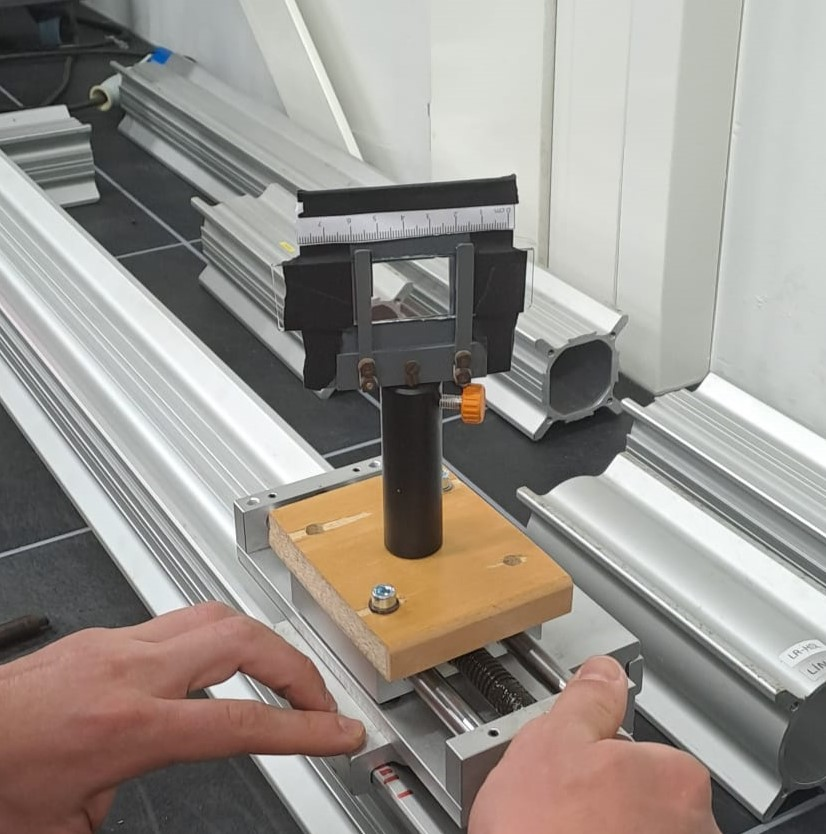
\includegraphics[width=0.5\textwidth]{figures/angled glass slider.jpeg}
    \caption{Picture of the angled glass in a linear slider, used to investigate the effect of $M_{ag}$ in the sensitivity}
    \label{fig: Angled Glass Slider}
\end{figure}

\subsection{Uncertainty Sources}
\label{subsection: angled glass uncertainty}

\par The campaign compares a displacement predicted by Equation \ref{equation: Displacement of angled glass} against a displacement measured by cross-correlation. Each side carries its own uncertainty, so two budgets are required before any disagreement between them can be interpreted. The defocus distance $l$ enters neither budget, since it cancels from the ratio of the predicted to the measured displacement. An error in $l$ can therefore not account for a disagreement between the two, although it does propagate into the sensitivity $S$.

\par Three quantities feed the prediction: the plate thickness $T$, the plate angle $\theta$ and the refractive index $n$. Thickness was measured with a calliper and the angle was set with a protractor. The refractive index was not measured and was taken from the value quoted for the glass, $n = 1.52 \pm 0.02$. Each input is treated as a rectangular distribution of half-width $a$, so its standard uncertainty is $u = a/\sqrt{3}$.

\par Sensitivity coefficients were obtained numerically from Equation \ref{equation: Displacement of angled glass} at both glass angles of the campaign. Table \ref{tab: angled glass uncertainty} collects them. The plate angle dominates. A deviation of $0.1^{\circ}$ moves the predicted displacement by 0.63\% at $\theta = 17^{\circ}$ and by 0.55\% at $\theta = 20^{\circ}$, whereas thickness and refractive index together account for less than half of the combined figure.

\begin{table}[h]
    \centering
    \caption{Uncertainty budget for the displacement predicted by Equation \ref{equation: Displacement of angled glass}. Each input is treated as a rectangular distribution of half-width $a$, so that $u = a/\sqrt{3}$. The last two columns give the relative contribution of each input to the predicted displacement at the two glass angles used in the campaign.}
    \label{tab: angled glass uncertainty}
    \begin{tabular}{llrrrr}
        \toprule
        Source & Instrument & $a$ & $u(x_i)$ & \multicolumn{2}{c}{Contribution [\%]} \\
        \cmidrule(lr){5-6}
               &            &     &          & $\theta = 17^{\circ}$ & $\theta = 20^{\circ}$ \\
        \midrule
        Plate thickness $T$  & Calliper   & 0.02 mm         & 0.012 mm         & 0.58 & 0.58 \\
        Refractive index $n$ & Literature & 0.02            & 0.012            & 1.40 & 1.37 \\
        Plate angle $\theta$ & Protractor & $0.50^{\circ}$  & $0.29^{\circ}$   & 1.82 & 1.59 \\
        \midrule
        Combined             &            &                 &                  & 2.37 & 2.18 \\
        \bottomrule
    \end{tabular}
\end{table}

\par Two quantities feed the measurement. The first is the scatter of the cross-correlation vector field $\sigma_\Delta$, already listed in Table \ref{tab: angled glass displacement results}, which runs from 2.0\% to 6.0\% of the mean displacement with an average of 3.2\%. The standard deviation of the field is used here in place of the standard error of the mean, because a 75\% window overlap leaves neighbouring vectors strongly correlated and the effective number of independent samples well below the vector count. The second is the optical magnification returned by the DaVis calibration, which converts the measured displacement from pixels to millimetres. \todo{insert the DaVis calibration fit residual}

\par The two budgets combine in quadrature to a standard uncertainty of approximately 4\% on the comparison between prediction and measurement, or 8\% at a coverage factor of $k = 2$. \todo{recompute once the calibration residual is available}

\par Three consequences follow for the results of Chapter \ref{chapter: Results}. Points 2 to 9 disagree by 0.5\% to 2.6\%, which falls below the standard uncertainty and calls for no further explanation. Point 1 shows the largest disagreement of the campaign at 7.9\%, close to twice the standard uncertainty and at the edge of the interval defined by $k = 2$. The value stays compatible with the budget as a whole, although no single input accounts for it on its own: an error in $\theta$ alone would have to reach $1.26^{\circ}$, which exceeds the reading uncertainty of the protractor by more than a factor of four. Points 10 to 20 sit between 2.4\% and 3.7\%, all of the same sign and with no dependence on $l$. A one-signed offset of this kind indicates a systematic error rather than scatter, and an angle offset of $0.57^{\circ}$ reproduces it exactly. Those eleven points share a single setting of the glass plate, so a small constant error in $\theta$ is the most plausible source.

\par No beam expander was used during the first experimental campaign. Since no specification in the literature was found to size the laser diffuser and given the small field of view of 2cm, it was believed that the scattering and diffusion alone from the ground glass would be sufficient to fill the whole field of view. However that belief was proven wrong. Moreover, the small size of the diffuser made the laser beam diffraction limited at the ground glass and not at the camera aperture, this meant that changing the f-stop of the camera had no effect in the average speckle pattern size and the average speckles were a lot bigger than expected. Another effect was the vignetting of the speckle pattern diameter, meaning that the pattern size would change with the aperture diameter and magnification ($D_{\Delta s} \approx D \cdot M_{ag}$), which limited the usable $f_\#$. Faced with these limitations, another experimental campaign was envisioned with a bigger ground glass and a beam expander to try and produce a finer speckle pattern.

\section{Speckle Pattern Investigation}
\label{section: Speckle Pattern Investigation}
The second experimental campaign was intended to investigate further the speckle pattern and tackle the limitations of the first experiments. The main goals were to better understand the creation of a finer speckle pattern that would not experience vignetting, assess how the average speckle size correlates to the Rayleigh limit of Equation \ref{equation: Rayleigh Limit} and also compare the generation of speckles through direct ground glass diffusion and by projecting the laser into a surface. The setup used for the direct speckles investigation resembles the one shown in Section \ref{section: Angled Glass Experiment} and can be seen in Figure \ref{fig: Directed speckles investigation setup}.

\begin{figure}[h]
    \centering
    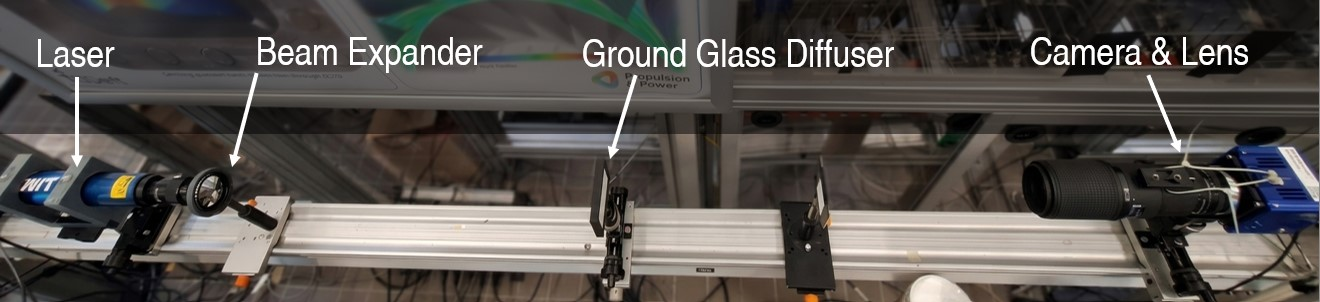
\includegraphics[width=\textwidth]{figures/speckle pattern investigation.jpg}
    \caption{Assembled directed speckle investigation setup. Configuration is quite similar from the one presented in Section \ref{section: Angled Glass Experiment} with the distinct presence of the beam expander lens in-between the laser and ground glass diffuser.}
    \label{fig: Directed speckles investigation setup}
\end{figure}

%%Modify this Picture ^^^ to show dgg and df

The main difference between the setup in Figure \ref{fig: Angled glass setup} and the one in Figure \ref{fig: Directed speckles investigation setup} is the presence of a larger ground glass diffuser and a lens to expand the laser beam. The new ground glass diffuser has 88 mm of length and 61 mm of width, which makes it capable of filling larger fields of view. The beam expander consists of a convergent lens with focal length of $f = 80$ mm, positioned at a distance $d_{GG}$ behind the ground glass, which was varied to see its effects in the speckle creation. The camera and laser are the same from the last experiment, only the camera lens with $f=200$mm was used.

A series of pictures were taken where $d_{GG}, M_{ag}$ and $f_\#$ were varied. Table \ref{tab: speckle investigation matrix} summarizes the experimental condition of each picture. The average speckle size was then computed using LaVision's DaVis 11 software processing function \emph{particle/speckle size over time} which computes the spatial averaged particle size through a defined sliding average length and subtracting the sliding minimum \cite{Pan2010}. For this application, both quantities were set to 16 pixels. These pictures will enable the selection of a ground glass distance capable of producing the desired speckle pattern, it will also quantify the effect of the magnification and f-stop number in the speckle production.

\begin{table}[h]
    \centering
    \caption{Configurations acquired during the speckle pattern investigation.
    $d_{GG}$ is the distance between the beam expander lens and the ground glass
    diffuser, $M_{ag}$ the magnification measured from the calibration and
    $\Delta s_{th}$ the speckle size predicted by the Rayleigh criterion
    (Equation \ref{equation: Rayleigh Limit}).}
    \label{tab: speckle investigation matrix}
    \begin{tabular}{lrrrrr}
        \toprule
        Point & $f_\#$ & $d_{GG}$ & $M_{ag}$ & $d_f$ & $\Delta s_{th}$ \\
              &         & [mm]     & [--] & [mm] & [px] \\
        \midrule
         1 &  4 & 740 & 0.9635 & 415 & 0.93 \\
         2 & 11 & 740 & 0.9635 & 415 & 2.57 \\
         3 & 22 & 740 & 0.9635 & 415 & 5.13 \\
         4 &  4 & 740 & 0.2956 & 930 & 0.62 \\
         5 & 11 & 740 & 0.2956 & 930 & 1.69 \\
         6 & 22 & 740 & 0.2956 & 930 & 3.39 \\
         7 & 11 & 450 & 0.2956 & 930 & 1.69 \\
         8 & 11 & 280 & 0.2956 & 930 & 1.69 \\
         9 & 11 & 190 & 0.2956 & 930 & 1.69 \\
        10 & 11 & 100 & 0.2956 & 930 & 1.69 \\
        11 &  4 & 300 & 0.4572 & 680 & 0.69 \\
        12 & 11 & 300 & 0.4572 & 680 & 1.90 \\
        13 & 22 & 300 & 0.4572 & 680 & 3.81 \\
        \bottomrule
    \end{tabular}
\end{table}

% This table is missing the experiments where we varied the zoom based on the lens indications, worth adding here (??) Definitely.

\begin{figure}[h]
    \centering
    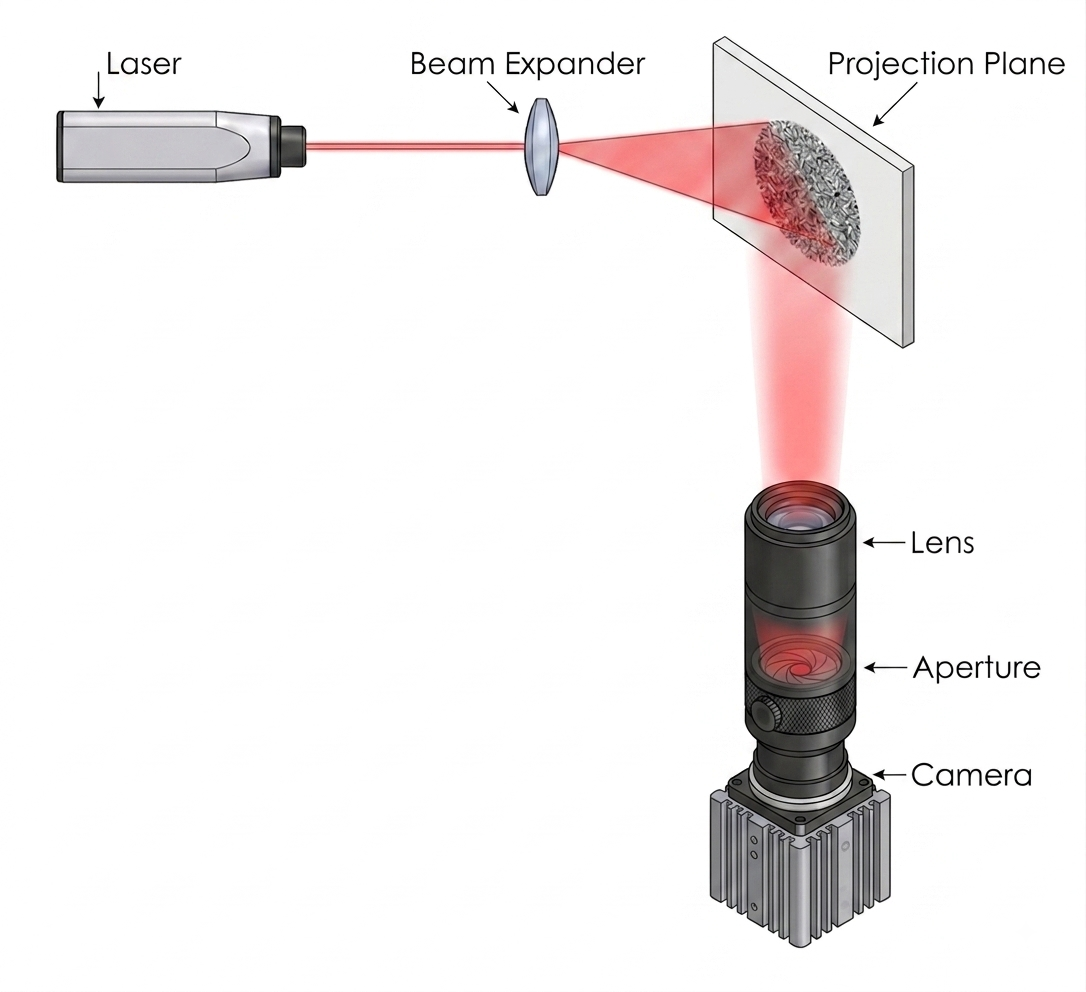
\includegraphics[width=0.5\textwidth]{figures/projected speckle schematic.png}
    \caption{Diagram of the setup used to create and study projected speckles}
    \label{fig: projected speckle setup diagram}
\end{figure}

The previous setup was modified to also test the creation of speckles by projecting the laser in a blank canvas, similar to what was done by Meier \& Rösgen and Bühlmann \cite{Meier&Roesgen2013,Buhlmann2020}. As shown by the schematic in Figure \ref{fig: projected speckle setup diagram}, a blank surface angled at $45^{\circ}$ has been placed in the beam path and the camera assembly has been moved to a perpendicular beam. The laser is expanded by the same $f=80$ mm lens. When it hits the surface, its light diffuses and creates an interference pattern captured by the camera. Figure \ref{fig: projected speckle experiment} shows a picture of the speckle pattern being generated in the projection plane, there it is also possible to see the camera assembly and the beam expander.


\begin{figure}[h]
    \centering
    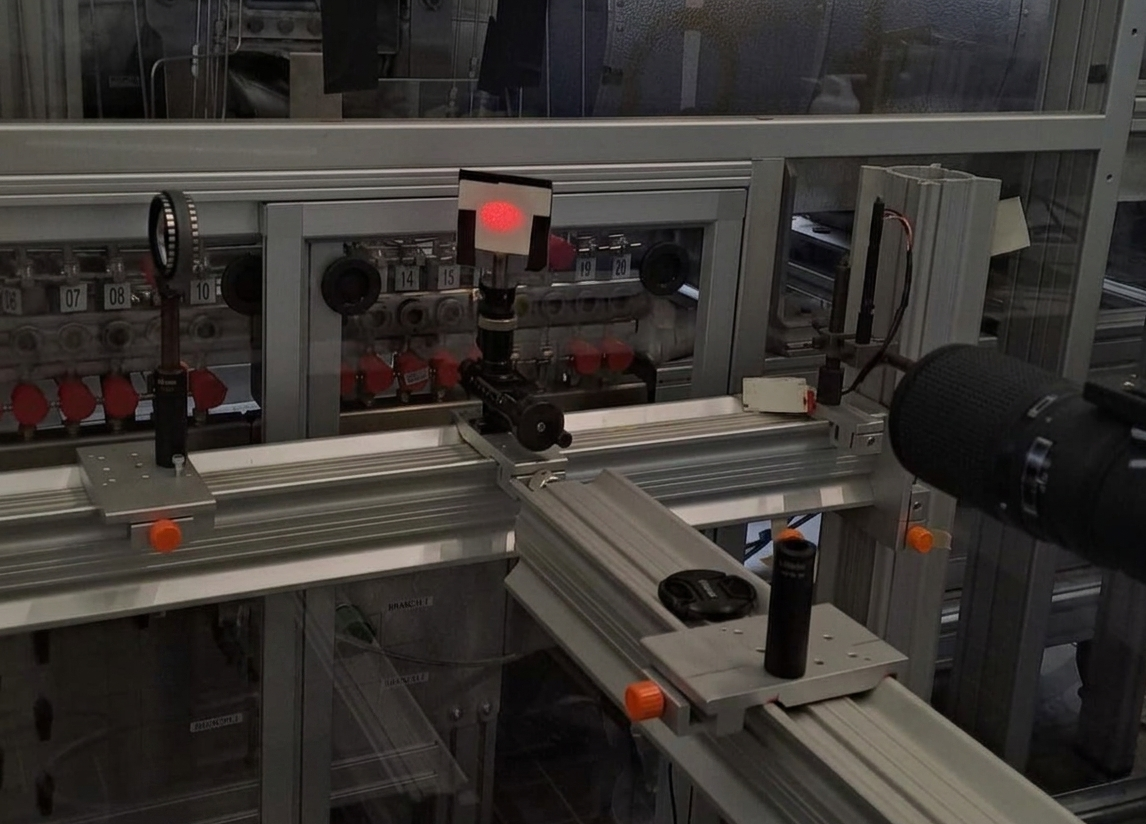
\includegraphics[width=0.7\textwidth]{figures/projected speckle pattern experiment.png}
    \caption{Photograph of the projected speckle experimental setup. In the projection plane it is possible to see the speckle pattern formed}
    \label{fig: projected speckle experiment}
\end{figure}

\subsection{Uncertainty Sources}
\label{subsection: speckle uncertainty}

\par This campaign sets a measured average speckle size against the Rayleigh limit of Equation \ref{equation: Rayleigh Limit}. The two quantities are not equivalent. Equation \ref{equation: Rayleigh Limit} returns the smallest speckle the optical system can form, whereas the DaVis function returns a spatial average over a real pattern. A measured value above the prediction is therefore the expected outcome, and the comparison tests a floor rather than an equality. Only a measured value below the limit would indicate an error.

\par The prediction rests on three inputs. The wavelength is fixed by the laser line at $\lambda = 632.8$ nm and contributes nothing of consequence. The optical magnification comes from the same DaVis calibration discussed in Subsection \ref{subsection: angled glass uncertainty}, so its uncertainty carries over unchanged. The f-stop number deserves attention, because the values engraved on a lens barrel are rounded members of a geometric series. Table \ref{tab: fstop correction} lists the effect. Marked apertures of 4, 8 and 16 are exact, whereas 11 and 22 stand for 11.31 and 22.63. The $\Delta s_{th}$ column of Table \ref{tab: speckle investigation matrix} is consequently low by 2.9\% for the ten points acquired at those two settings.

\begin{table}[h]
    \centering
    \caption{Effect of the rounded f-stop scale on the speckle size predicted by Equation \ref{equation: Rayleigh Limit}. The engraved values follow powers of $\sqrt{2}$, and two of the three settings of this campaign are rounded. The correction applies to every point of Table \ref{tab: speckle investigation matrix} acquired at $f_\# = 11$ or $f_\# = 22$.}
    \label{tab: fstop correction}
    \begin{tabular}{lrrl}
        \toprule
        Marked $f_\#$ & Actual $f_\#$ & Correction on $\Delta s_{th}$ & Points affected \\
        \midrule
        4  &  4.00 & 0.0\% & 1, 4, 11 \\
        11 & 11.31 & 2.9\% & 2, 5, 7, 8, 9, 10, 12 \\
        22 & 22.63 & 2.9\% & 3, 6, 13 \\
        \bottomrule
    \end{tabular}
\end{table}

\par On the measurement side the dominant term is the estimator itself. The DaVis function subtracts a sliding minimum from a sliding average, and both lengths were fixed at 16 pixels for every point of the campaign. That choice is arbitrary and the returned size depends on it. A repeat of the analysis at other lengths bounds the effect. \todo{repeat the speckle size analysis at 8 and 32 px and quote the spread}

\par Speckle formation is random in nature, as established in Chapter \ref{chapter: LiteratureReview}. A single image therefore yields a finite sample estimate rather than a fixed property of the setup, and the spread across the field or across repeated frames sets a statistical floor that no choice of estimator can improve upon. \todo{quote the standard deviation of the speckle size across the field}

\par One condition governs whether the comparison is meaningful at all. Section \ref{section: Angled Glass Experiment} established that the small diffuser of the first campaign made the beam diffraction limited at the ground glass instead of at the camera aperture, which placed the setup outside the regime that Equation \ref{equation: Rayleigh Limit} describes. The larger diffuser was introduced to restore that regime. Evidence for the restoration is the response of the measured size to the f-stop, since a diffraction limit set at the aperture must scale with $f_\#$ and one set at the diffuser must not. Points 1 to 3, 4 to 6 and 11 to 13 each hold the magnification fixed and vary only the aperture, so the three groups provide that test directly. Residual vignetting would break the same condition across the field and is checked by a comparison of the estimate between the centre and the edge of the image.

Up until now, the designed setup made it known how to create an appropriate speckle pattern and how to set the optical distances so a desirable sensitivity and spatial resolution is achieved. This knowledge now can be applied in a proof of concept case that enables the visualization of a true density gradient and even its integration into a density field. The next experiment will build on that basis to visualize a compressible jet, which will serve as proof of concept and allow for the reconstruction of a density field using SBOS.

\section{Compressible Jet Experiment}
\label{section: Compressible jet experiment}

A similar setup to the one shown in Figure \ref{fig: Directed speckles investigation setup} was used to image a compressible jet. For this experiment, $l = 3$ cm, $d_{GG} = 83$ cm, $d_f = 74$ cm and $f_\# = 11$, which gives $M_{ag} = 0.37$, $S = 11.1$ mm and $s_{min} = 0.369$ mm. Figure \ref{fig: Compressible Jet experiment} shows a picture of the assembled setup. The jet was achieved by connecting a standard air gun with a nozzle diameter $d_N = 3.5$ mm to a wall air tap with a hose. This setup allowed to adjust the pressure coming out of the air tap, however, a big limitation was the lack of loss quantification through the hose, quick-disconnect couplings and the air gun itself, meaning that the actual pressure right before the nozzle exit was unknown.

\begin{figure}[h]
    \centering
    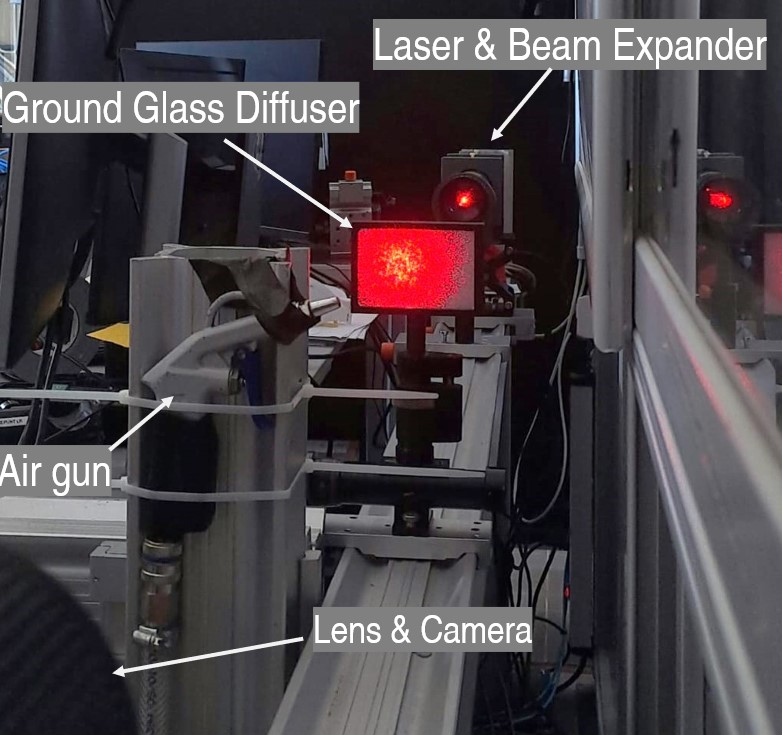
\includegraphics[width=0.5\textwidth]{figures/compressible jet setup.jpeg}
    \caption{Photograph of the compressible jet experimental setup.}
    \label{fig: Compressible Jet experiment}
\end{figure}

The data acquisition followed a similar procedure than the one explained at Section \ref{section: Angled Glass Experiment}. A target plate was put at the in-focus position and a picture was captured to calibrate laVision's DaVis software. Then, the laser was turned on and a reference picture was taken. The pressure was set at the air tap valve and the air gun was triggered, while the camera captured 100 images with an exposure time of 300 $\mu$s. In total, 6 cases were captured with pressures at the air tap valve ranging from 3 bar to 8 bar with 1 bar step. The speckle size obtained was checked following the procedure of Section \ref{section: Speckle Pattern Investigation}. The 100 images for each case were averaged and cross-correlated with an interrogation window of 12 px, 75\% of overlap and 4 multipasses.


\subsection{Uncertainty Sources}
\label{subsection: jet uncertainty}

\par The jet measurement runs through a longer chain than the two campaigns before it. A displacement field is converted into a deflection angle, the deflection angle into a density gradient through the Gladstone-Dale relation, and the gradient into a density field through the inverse Abel transform of Subsection \ref{subsection: Axisymmetric Refractive Field}. Every stage adds a term, and the terms fall into three groups: the flow condition, the optical setup, and the reconstruction.

\par The flow condition carries the largest uncertainty and the one least under control. As stated at the start of this section, the pressure at the air tap valve is known but the pressure immediately upstream of the nozzle is not, because the losses across the hose, the quick-disconnect couplings and the air gun body were never quantified. Any comparison against compressible flow theory inherits that gap, since the nozzle pressure ratio follows from the stagnation pressure alone. An independent route exists. The shock cell length of an underexpanded jet depends on the nozzle pressure ratio through the relation of Emden \cite{Emden1899}, so a measurement of the cell length recovers the pressure without a gauge at the nozzle. \todo{bound the nozzle pressure from the measured shock cell length}

\par The optical terms are those of Subsection \ref{subsection: angled glass uncertainty} and transfer without modification. Sensitivity follows from $S = l M_{ag}$, so the defocus distance and the calibration magnification enter directly. Both were set once for the whole pressure series, which makes their contribution a common bias across the six cases rather than a source of scatter between them. Relative comparisons between pressures are therefore tighter than the absolute density level.

\par Processing contributes a term that the current settings hide. The 100 frames of each case were averaged before cross-correlation, so the algorithm returns a single mean field and no estimate of its own repeatability. Correlation of the frames individually recovers that estimate, and the standard deviation across the 100 realisations then plays the role that $\sigma_\Delta$ plays in Table \ref{tab: angled glass displacement results}. The same operation separates measurement noise from genuine unsteadiness in the jet, which the average discards. \todo{correlate the frames individually and quote the scatter across realisations}

\par Three terms belong to the reconstruction. The Gladstone-Dale coefficient for air at $\lambda = 632.8$ nm is known to better than one percent and is negligible against the rest. The width assigned to the refractive object in the near-field correction is not measured but inferred, so its influence on the recovered density needs a sensitivity study across a plausible range. \todo{quantify the density sensitivity to the assumed object width} The inverse Abel transform assumes axial symmetry and involves a derivative, which amplifies noise towards the jet axis and makes the centreline density the least reliable part of the field. A jet from a commercial air gun nozzle is unlikely to be perfectly symmetric, and a comparison of the two halves of the measured field quantifies the departure.

\section{Aerospike Experiment}
\chapter{Results}
\label{chapter: Results}

% REVIEW: chapter introduction still a placeholder.
Write Introduction paragraph 

\section{Angled Glass Experiment Results}
\label{section: Angled Glass Experiment Results}
The Angled Glass Experiment aimed to validate the methodology and compare the different defocus configurations treated in Chapter \ref{chapter: methodology}. This section presents the data gathered, describes how it was treated, discusses the uncertainty of the results, and concludes whether these objectives have been achieved. The tables that follow give an overview of the results.

Table \ref{tab: angled glass displacement results} compares the displacements measured through SBOS with the predicted shift induced by the angled glass. $\Delta_x$ is the mean of the cross-correlation vector field in pixels, $\Delta x_{SBOS}$ is the latter transferred to mm in the focal plane and $\Delta x_{glass}$ is the glass-induced ray shift, calculated through Equation \ref{equation: Displacement of angled glass}. Since the glass piece produces a uniform displacement field, the standard deviation of the cross-correlation field $\sigma_\Delta$ quantifies the precision of the SBOS measurement, while the relative error quantifies the accuracy of the method. The last column displays the total combined uncertainty of measurement of $\Delta x$, which will be treated in more detail later this section.

The table allows the comparison of the measurement error with its inherent uncertainty. In general terms, the error obtained is below the combined uncertainty, with the exception of points 1, 17 and 18. Only point 1, however, differs significantly from the uncertainty, with a difference of 4.76 percentage points, while 17 and 18 deviate by less than 0.5 percentage points. Regarding point 1, an error of $1.26^{\circ}$ in the glass angle measurement would be needed to cause its deviation of 7.87\%, which exceeds the reading uncertainty of the protractor. The cause for such error could be a misread angle or an unnoticed movement that changed the angle when setting it in the rail.

% REVIEW: "every point except 1 stays ... below its measurement uncertainties" contradicts the previous paragraph, where points 17 and 18 exceed their uncertainty.
The slider experimental error is also worth a remark due to the distinct behavior of its deviation. As it can be seen in Table \ref{tab: angled glass displacement results}, all the deviations of the slider experiments are positive and have a similar magnitude, which leads to the interpretation of an induced bias in the measurement. It is not clear what caused this bias, although it could have been introduced by an error in the magnification added to one in the glass angle, as both were fixed throughout the measurements. Nevertheless, the deviation of every point except 1 stays well within 5\%, below its measurement uncertainties, and the scatter signaled by $\sigma_\Delta$ is well within 2px. Consequently, these metrics indicate that the technique has been well implemented and is capable of producing accurate and precise results.

%Alternative for the above paragraph
%Every point except point 1 falls within its own standard uncertainty, and points 17 and 18 are the only ones that require the interval defined by $k = 2$. The agreement is therefore better than the raw percentages suggest, since the points with the largest deviations are also the ones with the largest scatter. Point 1 is the exception at 7.87\%, which is 2.5 times its combined standard uncertainty of 3.11\%. The glass angle alone does not explain it, because an error of $1.26^{\circ}$ would be required and that value exceeds the reading uncertainty of the protractor by more than a factor of four. The most likely explanation is a combination of a misread angle and a plate that was not seated flat against its mount. not seated flat against it mount? What?


\begin{table}[h]
    \centering
    \caption{Displacements measured in the angled glass campaigns. $\Delta_x$ is the mean displacement returned by the cross-correlation, $\sigma_\Delta$ its standard deviation over the vector field, $\Delta x_{SBOS}$ is that displacement referred to the focal plane, $\Delta x_{glass}$ the value calculated by Equation \ref{equation: Displacement of angled glass} for a plate of thickness $T = 2$ mm and refractive index $n = 1.52$ at the measured angle $\theta$. The $\Delta x_{SBOS}$ dev. column is the relative deviation of the two. Points 1 to 9 follow the fixed field of view configurations of Table \ref{tab: angled glass test matrix}; points 10 to 20 follow the linear slider configurations of the same table. The column $u_{tot}$ gives the combined standard uncertainty of the comparison between $\Delta x_{SBOS}$ and $\Delta x_{glass}$ calculated from the budgets of Tables \ref{tab: angled glass uncertainty} and \ref{tab: measurement uncertainty}.}
    \label{tab: angled glass displacement results}
    \begin{tabular}{lrrrrrrr}
        \toprule
        Point & $\theta$ & $\Delta_x$ & $\sigma_\Delta$ & $\Delta x_{SBOS}$ & $\Delta x_{glass}$ & $\Delta x_{SBOS}$ dev. & $u_{tot}$ \\
              & [$^{\circ}$] & [px] & [px] & [mm] & [mm] & [\%] & [\%] \\
        \midrule
         1 & 17 & 29.818 & 0.6001 & 0.1933 & 0.2099 & $-7.87$ &  3.11 \\
         2 & 17 & 22.613 & 1.3660 & 0.2136 & 0.2099 & $+1.77$ &  6.49 \\
         3 & 17 & 34.355 & 0.8521 & 0.2137 & 0.2099 & $+1.84$ &  3.43 \\
         4 & 17 & 21.368 & 0.5763 & 0.2071 & 0.2099 & $-1.30$ &  3.59 \\
         5 & 17 & 33.414 & 0.7710 & 0.2082 & 0.2099 & $-0.78$ &  3.31 \\
         6 & 17 & 23.067 & 1.0230 & 0.2088 & 0.2099 & $-0.51$ &  5.03 \\
         7 & 20 & 41.386 & 1.8830 & 0.2552 & 0.2500 & $+2.05$ &  5.05 \\
         8 & 20 & 22.306 & 0.6617 & 0.2537 & 0.2500 & $+1.46$ &  3.68 \\
         9 & 20 & 25.238 & 0.7720 & 0.2565 & 0.2500 & $+2.59$ &  3.76 \\
        \midrule
        10 & 20 & 29.373 & 0.7733 & 0.2561 & 0.2500 & $+2.42$ &  3.42 \\
        11 & 20 & 29.432 & 0.8055 & 0.2566 & 0.2500 & $+2.63$ &  3.50 \\
        12 & 20 & 29.595 & 0.7575 & 0.2580 & 0.2500 & $+3.20$ &  3.36 \\
        13 & 20 & 29.613 & 0.7711 & 0.2582 & 0.2500 & $+3.26$ &  3.40 \\
        14 & 20 & 29.580 & 0.7661 & 0.2579 & 0.2500 & $+3.15$ &  3.39 \\
        15 & 20 & 29.662 & 0.8175 & 0.2586 & 0.2500 & $+3.43$ &  3.51 \\
        16 & 20 & 29.559 & 0.7815 & 0.2577 & 0.2500 & $+3.07$ &  3.43 \\
        17 & 20 & 29.653 & 0.7694 & 0.2585 & 0.2500 & $+3.40$ &  3.39 \\
        18 & 20 & 29.746 & 0.7815 & 0.2593 & 0.2500 & $+3.73$ &  3.41 \\
        19 & 20 & 29.653 & 0.8264 & 0.2585 & 0.2500 & $+3.40$ &  3.54 \\
        20 & 20 & 29.617 & 0.8570 & 0.2582 & 0.2500 & $+3.28$ &  3.62 \\
        \bottomrule
    \end{tabular}
\end{table}

Through Table \ref{tab: df and Mag angled glass results}, the design strategy of Chapter \ref{chapter: methodology} can be assessed. It presents a comparison of the optical distances and magnifications prescribed by the surface maps with the ones obtained through the focal plane calibration. In addition, the resulting $L_{FoV_{obj}}$ was compared with the enforced 17 mm field of view of the object. The table was restricted to the 9 points where the methodology of Chapter \ref{chapter: methodology} was used to size the optical setup. The relative magnification errors are all below 5\% with the exception of point 7. The latter was obtained using the minimum distance at which the calibration plate could be brought into focus when using an $f = 105$ mm lens. That distance was bigger than the one prescribed by the surface map, resulting in a large $d_f$, $M_{ag}$ and $L_{FoV_{obj}}$ error. The propagation of that error is also evident in the sensitivity shown in Table \ref{tab: sensitivity comparison}. Point 9 also deviates from the enforced field of view by more than 5\%, in this case by $-8.64$\%. It was acquired at $l = 150$ mm, the longest defocus distance of the campaign. Points 7 and 9 are therefore the two geometric extremes of the design space, the shortest focal length and the largest defocus, and they are also the only two points whose field of view falls outside 5\%. All remaining deviations are within that band, which signals the correct implementation of the method. The contribution of the optical magnification to the uncertainty was obtained through the maximum fit residual of the DaVis calibration and can be seen in Table \ref{tab: measurement uncertainty}.

\begin{table}[h]
    \centering
    \caption{Optical design values against measured values of the experimental campaign. $d_{f,th}$ and $M_{ag_{th}}$ are, respectively, the focal distance and optical magnification prescribed by the design methodology of Chapter \ref{chapter: methodology} and listed in Table \ref{tab: angled glass test matrix}. $M_{ag_{exp}}$ was measured with a calibration plate at the in-focus plane and $d_{f,exp}$ was calculated through $d_f = f(M_{ag_{exp}}+1)/M_{ag_{exp}}$. The $d_f$ and $M_{ag}$ deviation columns are the relative difference with respect to the design value. $L_{FoV_{obj}}$ is the field of view achieved at the refractive object, obtained from Equation \ref{equation: LFoVobj BOS} with the experimental magnification. Its deviation was taken with respect to the 17 mm $L_{FoV_{obj}}$ enforced during the design.}
    \label{tab: df and Mag angled glass results}
    \begin{tabular}{lrrrrrrrr}
        \toprule
        Point & $d_{f,th}$ & $d_{f,exp}$ & $d_f$ dev. & $M_{ag_{th}}$ & $M_{ag_{exp}}$ & $M_{ag}$ dev. & $L_{FoV_{obj}}$ & $L_{FoV_{obj}}$ dev. \\
              & [mm] & [mm] & [\%] & [--] & [--] & [\%] & [mm] & [\%] \\
        \midrule
        1 & 409.0 & 399.5 & $-2.32$ & 0.9561 & 1.0025 &  $+4.85$ & 16.81 & $-1.12$ \\
        2 & 505.0 & 490.6 & $-2.85$ & 0.6557 & 0.6882 &  $+4.96$ & 17.07 & $+0.43$ \\
        3 & 391.0 & 391.4 & $+0.11$ & 1.0498 & 1.0449 &  $-0.47$ & 16.87 & $-0.76$ \\
        4 & 511.0 & 498.2 & $-2.50$ & 0.6433 & 0.6706 &  $+4.24$ & 16.73 & $-1.56$ \\
        5 & 393.0 & 391.7 & $-0.32$ & 1.0369 & 1.0431 &  $+0.59$ & 16.21 & $-4.65$ \\
        6 & 490.0 & 478.5 & $-2.35$ & 0.6897 & 0.7181 &  $+4.12$ & 16.28 & $-4.22$ \\
        7 & 189.0 & 204.6 & $+8.25$ & 1.2500 & 1.0543 & $-15.66$ & 18.52 & $+8.97$ \\
        8 & 285.0 & 288.7 & $+1.30$ & 0.5831 & 0.5715 &  $-1.98$ & 17.76 & $+4.46$ \\
        9 & 527.0 & 512.7 & $-2.71$ & 0.6109 & 0.6395 &  $+4.69$ & 15.53 & $-8.64$ \\
        \bottomrule
    \end{tabular}
\end{table}

The data collected during the experimental campaign allows the assessment of sensitivity through two experimental routes. Table \ref{tab: sensitivity comparison} compares the theoretical sensitivity given by the surface map of Chapter \ref{chapter: methodology} to the sensitivity obtained through the geometry $S_{geom} = l \cdot M_{ag_{exp}}$ and the sensitivity obtained with the displacement data $S_\Delta = \Delta_x \cdot l_{px}/\varepsilon_{glass}$. With the exception of point 7, which has already been discussed, all data is within 8\% of agreement. It is worth noting that the $S_{geom}$ error is the same as the magnification error, while $S_\Delta$ stacks both the displacement measurement error and the geometric setup error. The total combined uncertainty of $S_\Delta$ has also been calculated and is displayed in the last column, most points are below $u_{tot}$ in magnitude or within 1\% to it with the exception of point 7 and 9. It is worth noting that most points whose error exceeds the total uncertainty belong to the slider experiment, which could have experienced a bias, as previously mentioned. Nevertheless, the data shows that the optical configuration parameters defined by the methodology of Chapter \ref{chapter: methodology} produce a setup with the predicted sensitivity within an acceptable error range. Therefore, it validates the methodology as it demonstrates that the physical setup reproduces the predicted performance.

\begin{table}[h]
    \centering
    \caption{Sensitivity obtained by two routes compared to theoretical sensitivity. $S_{th} = l M_{ag_{th}}$ is the design sensitivity of Table \ref{tab: angled glass test matrix}. $S_{geom} = l M_{ag_{exp}}$ is the sensitivity measured with the calibration plate, carrying the same deviation of Table \ref{tab: df and Mag angled glass results}. $S_{\Delta} = \Delta_x \cdot l_{px} / \varepsilon_{glass}$ follows from the displacements measured. The $S_{geom}$ dev. and $S_{\Delta}$ dev. columns give the deviation of $S_{geom}$ and $S_{\Delta}$ to $S_{th}$. The column $u_{tot}$ displays the combined standard uncertainty on $S_{\Delta}$ for each point, obtained from the budgets of Tables \ref{tab: angled glass uncertainty} and \ref{tab: measurement uncertainty}.}
    \label{tab: sensitivity comparison}
    \begin{tabular}{lrrrrrr}
        \toprule
        Point & $S_{th}$ & $S_{geom}$ & $S_{\Delta}$ & $S_{geom}$ dev. & $S_{\Delta}$ dev. & $u_{tot}$ \\
              & [mm] & [mm] & [mm] & [\%] & [\%] & [\%] \\
        \midrule
         1 &  76.5 &  80.2 &  73.9 &  $+4.84$ &  $-3.42$ &  3.19 \\
         2 &  52.5 &  55.1 &  56.0 &  $+4.87$ &  $+6.73$ &  6.53 \\
         3 & 105.0 & 104.5 & 106.4 &  $-0.49$ &  $+1.34$ &  3.48 \\
         4 &  64.3 &  67.1 &  66.2 &  $+4.29$ &  $+2.93$ &  3.64 \\
         5 &  83.0 &  83.4 &  82.8 &  $+0.54$ &  $-0.24$ &  3.39 \\
         6 &  55.2 &  57.4 &  57.2 &  $+4.08$ &  $+3.55$ &  5.08 \\
         7 & 100.0 &  84.3 &  86.1 & $-15.66$ & $-13.93$ &  5.10 \\
         8 &  46.6 &  45.7 &  46.4 &  $-1.88$ &  $-0.45$ &  3.75 \\
         9 &  91.6 &  95.9 &  98.4 &  $+4.73$ &  $+7.44$ &  3.78 \\
        \midrule
        10 &   0.0 &   0.0 &   0.0 &  --   &  -- &    -- \\
        11 &   7.4 &   7.5 &   7.7 &  $+0.75$ &  $+3.40$ &  6.75 \\
        12 &  14.8 &  14.9 &  15.4 &  $+0.75$ &  $+3.97$ &  4.43 \\
        13 &  22.2 &  22.4 &  23.1 &  $+0.75$ &  $+4.04$ &  3.90 \\
        14 &  29.6 &  29.8 &  30.8 &  $+0.75$ &  $+3.92$ &  3.68 \\
        15 &  37.0 &  37.3 &  38.6 &  $+0.75$ &  $+4.21$ &  3.70 \\
        16 &   7.4 &   7.5 &   7.7 &  $+0.75$ &  $+3.85$ &  6.71 \\
        17 &  14.8 &  14.9 &  15.4 &  $+0.75$ &  $+4.18$ &  4.45 \\
        18 &  22.2 &  22.4 &  23.2 &  $+0.75$ &  $+4.50$ &  3.92 \\
        19 &  29.6 &  29.8 &  30.8 &  $+0.75$ &  $+4.18$ &  3.82 \\
        20 &  37.0 &  37.3 &  38.5 &  $+0.75$ &  $+4.05$ &  3.80 \\
        \bottomrule
    \end{tabular}
\end{table}

\par Tables \ref{tab: angled glass displacement results} and \ref{tab: sensitivity comparison} both show total uncertainties that were obtained to better assess the measurement error. These values were computed through uncertainty budgets following the Guide to the Expression of Uncertainty in Measurement \cite{JCGM2008}. The campaign compared a displacement obtained by Equation \ref{equation: Displacement of angled glass} against the displacement measured by cross-correlation. Therefore, two budgets were constructed, one for the glass displacement and another for the CC measurement. Afterwards, the collected uncertainties were combined to obtain the sensitivity uncertainty. A description of each budget and the formulas used to assess the total contribution follows.

The glass displacement's uncertainty budget is summarized in Table \ref{tab: angled glass uncertainty}. It focuses on the three inputs of the angled glass displacement estimate, namely the plate thickness $T$, the plate angle $\theta$ and the refractive index $n$. Thickness was measured with a caliper and the angle was set with a protractor, while the refractive index was obtained from the literature for common glass. Each input was treated as a rectangular probability distribution of half-width $a$ with a standard uncertainty of $u = a/\sqrt{3}$. The sensitivity coefficients and contributions of each input variable regarding the two glass angles were also estimated based on Equation \ref{equation: Displacement of angled glass}. These coefficients measure how much a change in each variable affects the final displacement. They are also used to calculate the contribution of each variable to the combined uncertainty as it is equal to the sensitivity coefficient times uncertainty \cite{JCGM2008}. These quantities are presented in Table \ref{tab: angled glass uncertainty}, where the half-width and the standard uncertainty are listed for every input, followed by its contribution at each glass angle. The combined uncertainty for each angle is given at the bottom row and corresponds to the root of the sum of squares of the above percentages.

\begin{table}[htbp]
    \centering
    \caption{Uncertainty budget for the displacement predicted by Equation \ref{equation: Displacement of angled glass}. The three input variables are described under the Source column together with the instrument used to measure them in the instrument column. Each input is treated as a rectangular distribution of half-width $a$, so that $u = a/\sqrt{3}$ \cite{JCGM2008}. The contributions $c_i$ are the sensitivity coefficients, computed by inspecting the deviation in $\Delta x_{glass}$ after a small difference of each variable, multiplied by the uncertainty $u$. On the bottom row, the combined uncertainty of $\Delta x_{glass}$ can be found together with the formula used to compute it.}
    \label{tab: angled glass uncertainty}
    \begin{tabular}{llrrrr}
        \toprule
        Source & Instrument & $a$ & $u$ & \multicolumn{2}{c}{Contribution $c_i$ [\%]} \\
        \cmidrule(lr){5-6}
               &            &     &          & $\theta = 17^{\circ}$ & $\theta = 20^{\circ}$ \\
        \midrule
        Plate thickness $T$  & Caliper    & 0.02 mm         & 0.012 mm         & 0.58 & 0.58 \\
        Refractive index $n$ & Literature & 0.02            & 0.012            & 1.40 & 1.37 \\
        Plate angle $\theta$ & Protractor & $0.50^{\circ}$  & $0.29^{\circ}$   & 1.82 & 1.59 \\
        \midrule
        Combined, $u_{glass} = \sqrt{c_T^2 + c_n^2 + c_\theta^2}$             &            &                 &                  & 2.37 & 2.18 \\
        \bottomrule
    \end{tabular}
\end{table}

\par Regarding the uncertainty of the cross-correlation displacement measurement, it is affected mainly by two variables. The first is the scatter of the cross-correlation vector field $\sigma_\Delta$, listed in Table \ref{tab: angled glass displacement results}. It ranges from 2.0\% to 6.0\% of the mean displacement with an average of 3.0\%. This term is evaluated from the vector field itself, varying from point to point. The second is the optical magnification returned by the DaVis calibration. The calibration fit residual stayed within 2.9 px over the sensor width of 2560 px, which gives a contribution of 0.11\%. The pixel pitch $l_{px}$ is fixed by the manufacturer and is negligible against the other two. Table \ref{tab: measurement uncertainty} presents the second budget, together with the uncertainty of the defocus distance $l$, which is required for the sensitivity.

\begin{table}[htbp]
    \centering
    \caption{Uncertainty budget for the displacement measured by cross-correlation and sensitivity. The scatter of the vector field is evaluated from the data of Table \ref{tab: angled glass displacement results} and varies per point. For the magnification, DaVis calibration residual was used as its uncertainty which slightly varies per point, so the maximum was taken here. The pixel pitch is common to the whole campaign. The defocus distance was obtained with a metric tape and judged by about $\pm$ 1mm. The contributions were obtained as explained in Table \ref{tab: angled glass uncertainty}. The bottom rows show the combined uncertainty for $\Delta x$ and $S_\Delta$ together with the formulas used to compute them. Since the values vary per point, its range is presented here but they can be found in Tables \ref{tab: angled glass displacement results} and \ref{tab: sensitivity comparison}, respectively.}
    \label{tab: measurement uncertainty}
    \begin{tabular}{llrrr}
        \toprule
        Source & Instrument & $a$ & $u$ & Contribution $c_i$ [\%] \\
        \midrule
        Vector field scatter $\sigma_\Delta$        & Cross-correlation & --     & per point & 2.01 to 6.04 \\
        Optical magnification $M_{ag}$              & DaVis calibration & --     & 2.9 px    & 0.11 \\
        Pixel pitch $l_{px}$                        & Manufacturer      & --     & --        & negligible \\
        Defocus distance $l$                        & Metric tape       & 1 mm   & 0.58 mm   & 0.38 to 5.77 \\
        \midrule
        Combined, $u_{\Delta x} = \sqrt{u_{glass}^2+\sigma_{rel}^2 + c_{M_{ag}}^2 }$             &  &  &  & 3.11 to 6.49 \\
        Combined, $u_{S_\Delta} = \sqrt{u_{glass}^2+\sigma_{rel}^2 + c_{l}^2 }$  &  &  &  & 3.19 to 6.75 \\
        \bottomrule
    \end{tabular}
\end{table}


\par The total uncertainties that follow from the budgets are reported per point in the last column of their respective tables. The first total concerns the comparison between the predicted and the measured displacement. It combines the prediction budget with the scatter and the magnification, and it ranges from 3.11\% at point 1 to 6.49\% at point 2. The second total concerns the sensitivity $S_{\Delta}$, which stays within 3.19\% to 6.75\%. It reaches its largest values at points 11 and 16, for which the defocus distance of only 10 mm makes the contribution of $l$ dominant. Points 2, 6 and 7 sit above 5\% in both totals. In each case the cross-correlation scatter is the dominant contribution.

% REVIEW: points 7 and 8 used the f = 105 mm lens (Table 6.2), so they cannot be among the f = 200 mm points of Figure 6.1(a). State which points are plotted.
Regarding the research objectives, one of the goals of the experimental campaign was the comparison of the new capacities of SBOS to a standard BOS configuration. With the data at hand it is possible to compare the performance of a setup that uses negative defocus to another with positive defocus, effectively answering the experiment's objective. Figure \ref{fig: S vs l experimental} plots the sensitivity versus defocus distance of points 1 to 9 that were captured with $f=200$ mm, with error bars corresponding to the standard deviation divided by the mean cross-correlation displacement times the sensitivity values.

\begin{figure}[h]
    \centering
    \begin{subfigure}[b]{0.49\textwidth}
        \centering
        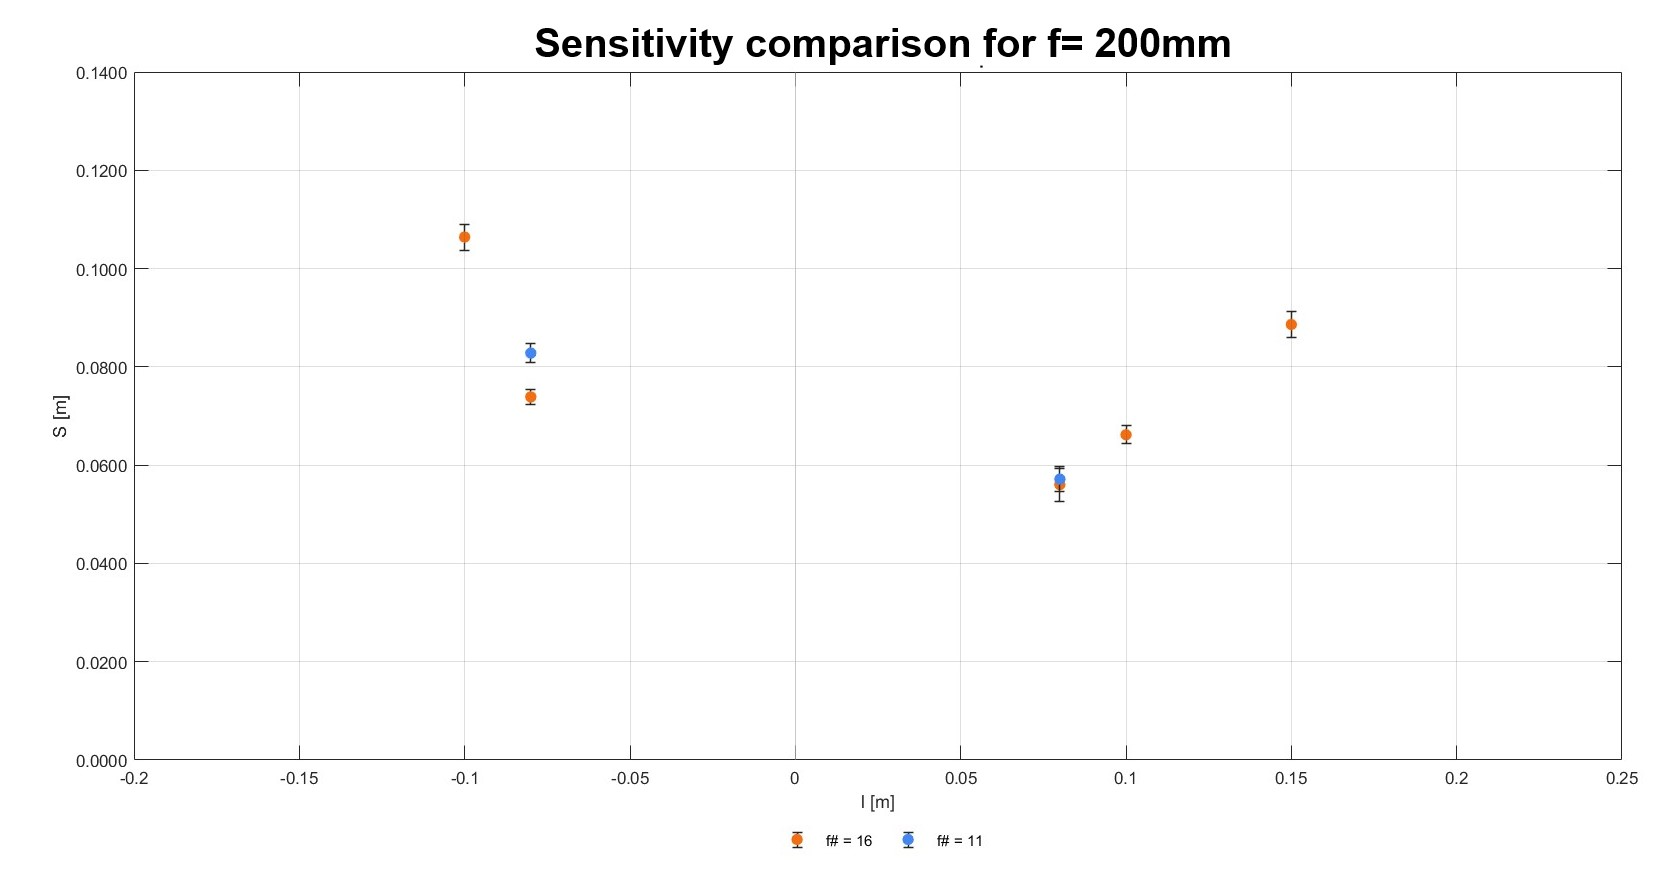
\includegraphics[width=\textwidth]{figures/S vs l experimental.jpg}
        \caption{}
        \label{fig: S vs l experimental}
    \end{subfigure}
    \hfill
    \begin{subfigure}[b]{0.49\textwidth}
        \centering
        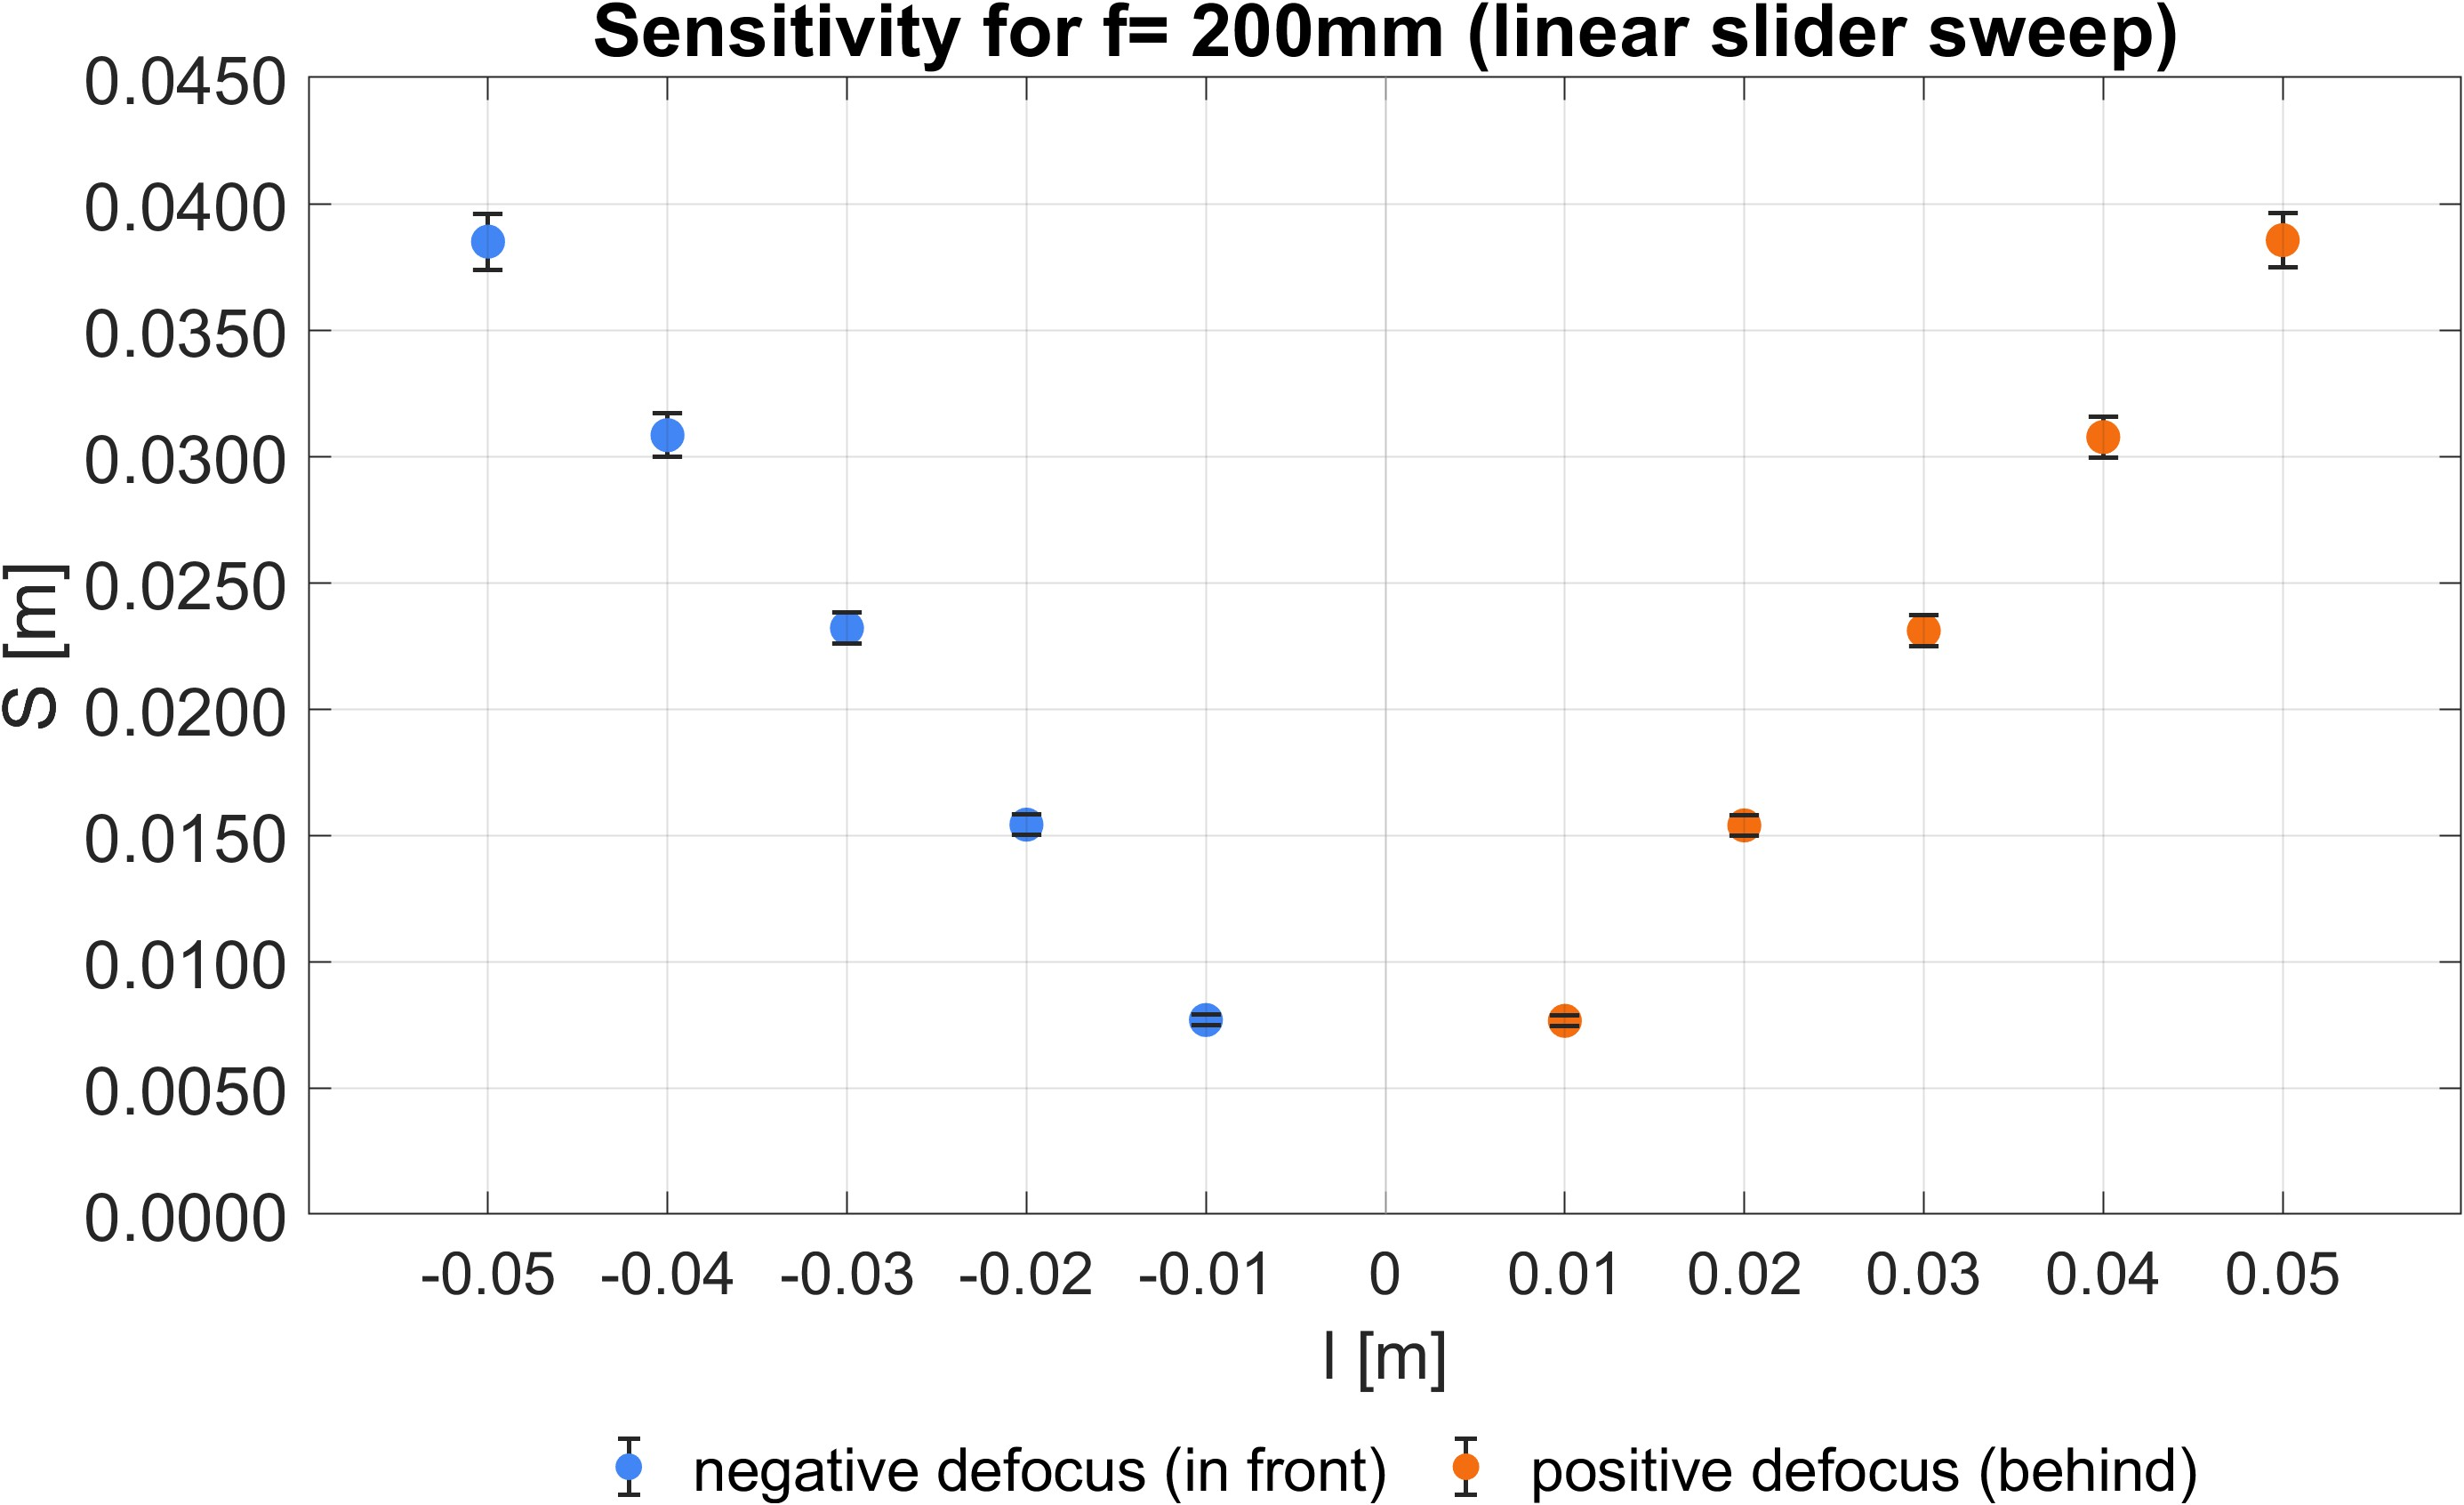
\includegraphics[width=\textwidth]{figures/S vs l slider experiment.jpg}
        \caption{}
        \label{fig: S vs l slider experiment}
    \end{subfigure}
    \caption{Sensitivity versus defocus distance for a camera lens of $f = 200$ mm. (a) Points obtained with $f_\# = 11$ and $f_\# = 16$ for an enforced $L_{FoV_{obj}} = 17$ mm. (b) Points obtained in the slider experiment, with a fixed measured magnification of $M_{ag} = 0.746$}
    \label{fig: S vs l experiments}
\end{figure}

Figure \ref{fig: S vs l experimental} replicates one of the predictions of Chapter \ref{chapter: methodology}, where a higher sensitivity was obtained for the same defocus distance if a negative defocus was chosen instead of its positive one. It is also worth noting that all points were obtained with the same field of view of the object. Therefore, a higher sensitivity and magnification are achieved while capturing the same area of the object. Although the resolution has not been measured in this case, it is also to be expected through Equation \ref{equation: S over smin} that the spatial resolution trade-off is improved by this increase in magnification. This figure effectively compares the performance of SBOS with BOS, answering one of the research questions posed in Chapter \ref{chapter: introduction}.


% REVIEW: the last two sentences say the same thing. The second one says "shorter focal length", but f was fixed; the quantity that changes is the focal distance d_f. "More powerful" is vague, consider "more sensitive".
Points 10 to 20 of Tables \ref{tab: angled glass displacement results} and \ref{tab: sensitivity comparison} show the results of the experiment where the angled glass was positioned in a linear slider with a fixed magnification and only the defocus position was changed. Figure \ref{fig: S vs l slider experiment} plots the resulting sensitivity against the defocusing distance. The points are symmetric around the Y-axis, which means that the mechanism that makes a negative defocus configuration more powerful than its positive counterpart is not the negative distance per se but the increased magnification that comes with a shorter focal distance to the camera. Therefore, the mechanism making negative defocus more sensitive than standard defocus is the higher magnification that comes with a shorter focal length.

% REVIEW: Chapter 4 presents Equation 4.9 as the minimum speckle size, here it is the predicted average size. The discrepancy is not only "at some points": every point exceeds the prediction by at least a factor of four.
Section \ref{section: Angled Glass Experiment} mentioned a discrepancy between the predicted average speckle size obtained through the Rayleigh diffraction limit and the ones obtained experimentally and computed using Hamarová's method \cite{Hamarova2016}. Table \ref{tab: angled glass speckle results} displays both quantities side by side together with the $f_\#$ and $M_{ag}$ used at each point. The $\Delta s$ deviation shows that at some points the discrepancy exceeds the theoretical value several times. Speckle formation is an intrinsically random phenomenon, described by complex physics \cite{Goodman2020, NikitaFominBook, Cloud2007}, so it is not exactly clear what is precisely the root of this difference. Nevertheless, the data gives some clues on what could be improved.

% REVIEW: this section finds that the speckle size follows M_ag and ignores f#, while Section 6.2 finds the opposite. Consider one paragraph that names both regimes. The mechanism is also stated three ways: imaged phase cells at the diffuser (here), laser diffraction limited in the diffuser (section summary) and small beam on the diffuser (Section 6.2). Pick one.
It seems that the f-stop number did not influence the average speckle size obtained experimentally. This becomes evident from observing points 4 and 8--10. In these points, the $f_\#$ ranges from 4 to 16 whereas $\Delta s$ stays within 12.35 px to 12.94 px. In contrast, changes in magnification were observed to have an effect in the experimental average speckle size considerably. From points 1--4 the $f_\#$ is fixed and $M_{ag}$ changes from 0.671 to 1.045, displaying $\Delta s$ from 12.74 px to 21.21 px. These factors contradict the Rayleigh equation for subjective speckles where its size is only dependent on the light's wavelength, imaging lens $f_\#$ and $M_{ag}$. The independence to the aperture size indicates that the interference pattern is not being created at the lens pupil as it should \cite{Goodman2020}. The magnification effect, in turn, means that the speckle is behaving like an imaged object. These factors lead to the belief that the pattern did not form a Rayleigh distribution at the lens pupil, rather what is being imaged are just the phase cells illuminated at the diffuser.

%This is a stretch from Goodman "If the diffuser overfills the projection lens, then each projector resolution cell undergoes a random walk of amplitudes scattered from the diffuser, resulting in an independent Rayleigh-distributed amplitude and uniformly distributed phase for each of such projection-lens resolution cells incident on the screen."


\begin{table}[htbp]
    \centering

% REVIEW: Delta s_th was computed with the design magnification (point 1: 3.72 px with M_th = 0.956, 3.80 px with M_exp = 1.002), but the column shows M_ag_exp. Recompute or state it in the caption.
    \caption{Speckle sizes measured during the angled glass campaign, for the configurations of Table \ref{tab: angled glass test matrix}. $M_{ag_{exp}}$ is the magnification measured with the calibration plate, $\Delta s_{th}$ the size predicted by the Rayleigh limit of Equation \ref{equation: Rayleigh Limit} and $\Delta s_{exp}$ the size returned by the one-dimensional autocorrelation method of Hamarová et al. \cite{Hamarova2016}, taken as the lag at which the normalised autocorrelation of intensity falls to $1/e$. The last column is the difference between the two. Points 11 to 20 share the optical layout of point 10, so their predicted and measured sizes are identical and have been omitted.}
    \label{tab: angled glass speckle results}
    \begin{tabular}{lrrrrr}
        \toprule
        Point & $f_\#$ & $M_{ag_{exp}}$ &  $\Delta s_{th}$ & $\Delta s_{exp}$ & $\Delta s$ dev. \\
              & [--] & [--] & [px] & [px] & [px] \\
        \midrule
         1 & 16.00 & 1.002 &   3.72 &  20.30 & $+16.58$ \\
         2 & 16.00 & 0.688 &   3.15 &  13.05 & $+9.90$ \\
         3 & 16.00 & 1.045 &   3.90 &  21.21 & $+17.31$ \\
         4 & 16.00 & 0.671 &   3.12 &  12.74 & $+9.62$ \\
         5 & 11.31 & 1.043 &   2.74 &  20.78 & $+18.04$ \\
         6 & 11.31 & 0.718 &   2.27 &  14.12 & $+11.85$ \\
         7 & 11.31 & 1.054 &   3.02 &  25.32 & $+22.30$ \\
         8 &  4.00 & 0.572 &   0.75 &  12.35 & $+11.60$ \\
         9 & 16.00 & 0.640 &   3.06 &  12.65 & $+9.59$ \\
        10 &  8.00 & 0.746 &   1.65 &  12.94 & $+11.29$ \\
        \bottomrule
    \end{tabular}
\end{table}


% REVIEW: the mechanism given here (laser diffraction limited in the diffuser) differs from the one in the speckle paragraph above and from the one in Section 6.2.
In this section, the results, errors and associated uncertainties of the angled glass experiments have been presented. The two plots constructed with the data collected permit answering one of this thesis' research questions and infer the mechanism that explains the advantage in performance of SBOS in comparison to BOS. Nevertheless, there was one prediction from theory that could not be verified in this experimental campaign: the average speckle size given by Rayleigh diffraction. The speckles obtained were considerably larger and did not change with the lens f-stop number, which led to the belief that the laser ray was becoming diffraction limited in the ground glass diffuser instead of the lens pupil. Another experimental campaign was envisioned to try and obtain a finer speckle pattern before the implementation of SBOS to a wind-tunnel application.


\section{Speckle Pattern Investigation Results}
\label{section: Speckle Pattern Experiment Results}

Faced with the difficulties in creating a satisfactory speckle pattern in the first experimental campaign, the second experiment aimed to investigate ways to generate a finer average speckle size, try to produce a Rayleigh distribution at the lens pupil and compare the implications of generating a speckle through direct diffusion or by projecting the laser into a surface. Table \ref{tab: speckle results} presents the data obtained with the experimental setups described in Section \ref{section: Speckle Pattern Investigation} with the conditions displayed in Tables \ref{tab: speckle investigation matrix} for direct speckles and \ref{tab: projected speckle matrix} for projected speckles. This section discusses the computed average speckle sizes obtained at each point, the deviation from the Rayleigh limit of Equation \ref{equation: Rayleigh Limit} and a quantification of the experiment's associated uncertainties.


%The main goals were to better understand the creation of a finer speckle pattern assess how the average speckle size correlates to the Rayleigh limit of Equation \ref{equation: Rayleigh Limit} and also compare the generation of speckles through direct ground glass diffusion and by projecting the laser into a surface.

\begin{table}[htbp]
    \centering
% REVIEW: Delta s_th of points 1-13 and 29-31 uses the design magnification (point 29: 0.67 px with M = 0.417, 0.69 px with M_exp = 0.457). The caption says M_ag_exp was measured with the calibration plate, but the magnification sweep figure says points 14-28 used the lens distance marks, and that uncertainty is not in the budget.
    \caption{Speckle sizes measured during the experimental campaign, using the optical configurations of Table \ref{tab: speckle investigation matrix}. $M_{ag_{exp}}$ is the magnification measured with the calibration plate, $\Delta s_{th}$ is the size predicted by the Rayleigh limit and $\Delta s_{exp}$ is the estimated experimental size, reported both by the DaVis function and by the method of Hamarová et al. \cite{Hamarova2016}. The deviation columns give the difference of each measurement from the prediction. The column $u_{tot}$ is the combined standard uncertainty of $\Delta s_{exp}$. Points 1 to 13 vary the aperture and the ground glass distance, whereas points 14 to 28 hold both fixed and sweep the magnification. Points 29 to 31 were obtained with projected speckles, using the parameters of Table \ref{tab: projected speckle matrix}.}
    \label{tab: speckle results}
    \begin{tabular}{lrrrrrrrrr}
        \toprule
        Point & $f_\#$ & $d_{GG}$ & $M_{ag_{exp}}$ & $\Delta s_{th}$ & \multicolumn{3}{c}{Hamarová} & \multicolumn{2}{c}{DaVis} \\
        \cmidrule(lr){6-8} \cmidrule(lr){9-10}
              & [--] & [mm] & [--] & [px] & $\Delta s_{exp}$ & $\Delta s$ dev. & $u_{tot}$ & $\Delta s_{exp}$ & $\Delta s$ dev. \\
              &      &      &      &      & [px] & [px] & [\%] & [px] & [px] \\
        \midrule
         1 &  4.00 &  740 & 0.964 &  0.92 &  1.74 &  $+0.82$ &  6.35 &   1.20 &  $+0.28$ \\
         2 & 11.31 &  740 & 0.964 &  2.59 &  2.73 &  $+0.14$ &  1.50 &   1.48 &  $-1.11$ \\
         3 & 22.63 &  740 & 0.964 &  5.19 &  3.83 &  $-1.36$ & 11.45 &   2.00 &  $-3.19$ \\
         4 &  4.00 &  740 & 0.296 &  0.61 &  1.62 &  $+1.02$ &  2.62 &   1.19 &  $+0.59$ \\
         5 & 11.31 &  740 & 0.296 &  1.71 &  2.71 &  $+1.00$ &  7.11 &   1.56 &  $-0.15$ \\
         6 & 22.63 &  740 & 0.296 &  3.42 &  3.81 &  $+0.39$ &  4.87 &   2.04 &  $-1.39$ \\
         7 & 11.31 &  450 & 0.296 &  1.71 &  2.29 &  $+0.58$ &  6.60 &   1.35 &  $-0.36$ \\
         8 & 11.31 &  280 & 0.296 &  1.71 &  2.45 &  $+0.74$ &  2.87 &   1.40 &  $-0.31$ \\
         9 & 11.31 &  190 & 0.296 &  1.71 &  2.91 &  $+1.20$ &  2.79 &   1.59 &  $-0.12$ \\
        10 & 11.31 &  100 & 0.296 &  1.71 &  4.59 &  $+2.88$ &  3.12 & failed &       -- \\
        11 &  4.00 &  300 & 0.877 &  0.88 &  2.42 &  $+1.54$ &  1.50 &   1.45 &  $+0.57$ \\
        12 & 11.31 &  300 & 0.877 &  2.49 &  2.98 &  $+0.49$ &  1.50 &   1.67 &  $-0.82$ \\
        13 & 22.63 &  300 & 0.877 &  4.97 &  4.15 &  $-0.83$ &  1.55 &   2.41 &  $-2.56$ \\
        \midrule
        14 & 22.63 &  300 & 1.000 &  5.37 &  3.05 &  $-2.33$ &  1.52 &   1.81 &  $-3.57$ \\
        15 & 22.63 &  300 & 0.909 &  5.13 &  3.14 &  $-1.99$ &  1.50 &   1.76 &  $-3.38$ \\
        16 & 22.63 &  300 & 0.800 &  4.84 &  3.26 &  $-1.58$ &  1.50 &   1.86 &  $-2.98$ \\
        17 & 22.63 &  300 & 0.667 &  4.48 &  2.66 &  $-1.81$ &  6.43 &   1.60 &  $-2.88$ \\
        18 & 22.63 &  300 & 0.571 &  4.22 &  2.80 &  $-1.42$ &  4.78 &   1.65 &  $-2.57$ \\
        19 & 22.63 &  300 & 0.500 &  4.03 &  2.39 &  $-1.64$ &  2.80 &   1.47 &  $-2.56$ \\
        20 & 22.63 &  300 & 0.400 &  3.76 &  3.60 &  $-0.16$ &  2.39 &   1.68 &  $-2.08$ \\
        21 & 22.63 &  300 & 0.333 &  3.58 &  2.16 &  $-1.42$ &  4.13 &   1.42 &  $-2.16$ \\
        22 & 22.63 &  300 & 0.286 &  3.46 &  2.38 &  $-1.07$ &  3.39 &   1.48 &  $-1.97$ \\
        23 & 22.63 &  300 & 0.222 &  3.28 &  2.53 &  $-0.76$ &  4.66 &   1.59 &  $-1.70$ \\
        24 & 22.63 &  300 & 0.167 &  3.13 &  2.88 &  $-0.25$ &  3.33 &   1.74 &  $-1.39$ \\
        25 & 22.63 &  300 & 0.118 &  3.00 &  3.06 &  $+0.06$ &  3.42 &   1.91 &  $-1.09$ \\
        26 & 22.63 &  300 & 0.074 &  2.89 &  2.72 &  $-0.17$ &  3.05 &   1.65 &  $-1.23$ \\
        27 & 22.63 &  300 & 0.054 &  2.83 &  2.76 &  $-0.07$ &  1.82 &   1.71 &  $-1.12$ \\
        28 & 22.63 &  300 & 0.035 &  2.78 &  3.09 &  $+0.31$ &  5.47 &   1.87 &  $-0.91$ \\
        \midrule
        29 &  4.00 &  300 & 0.457 &  0.67 &  1.59 &  $+0.92$ &  1.54 &   1.22 &  $+0.55$ \\
        30 & 11.31 &  300 & 0.457 &  1.90 &  2.21 &  $+0.31$ &  1.80 &   1.44 &  $-0.46$ \\
        31 & 22.63 &  300 & 0.457 &  3.81 &  3.61 &  $-0.20$ &  2.08 &   2.09 &  $-1.72$ \\
        \bottomrule
    \end{tabular}
\end{table}

Table \ref{tab: speckle results} and Figure \ref{fig: speckle size per point} show the average speckle size obtained experimentally for each point. They present the experimental speckle sizes obtained using DaVis' function together with the ones computed through Hamarová et al.'s autocorrelation method \cite{Hamarova2016}. A comparison between the two methods yielded some differences in magnitudes, with DaVis ranging from 1.19 to 2.41 px, while the autocorrelation spans from 1.59 to 4.59 px. Despite this difference, both methods reproduce the same trends reliably as shown by Figure \ref{fig: speckle size per point}. Since it is known how the estimator of Hamarová et al. works, contrary to the DaVis estimator, and both reproduce the same behavior, from now on the discussion will focus only on the results obtained with the autocorrelation method.

\begin{figure}[htbp]
    \centering
    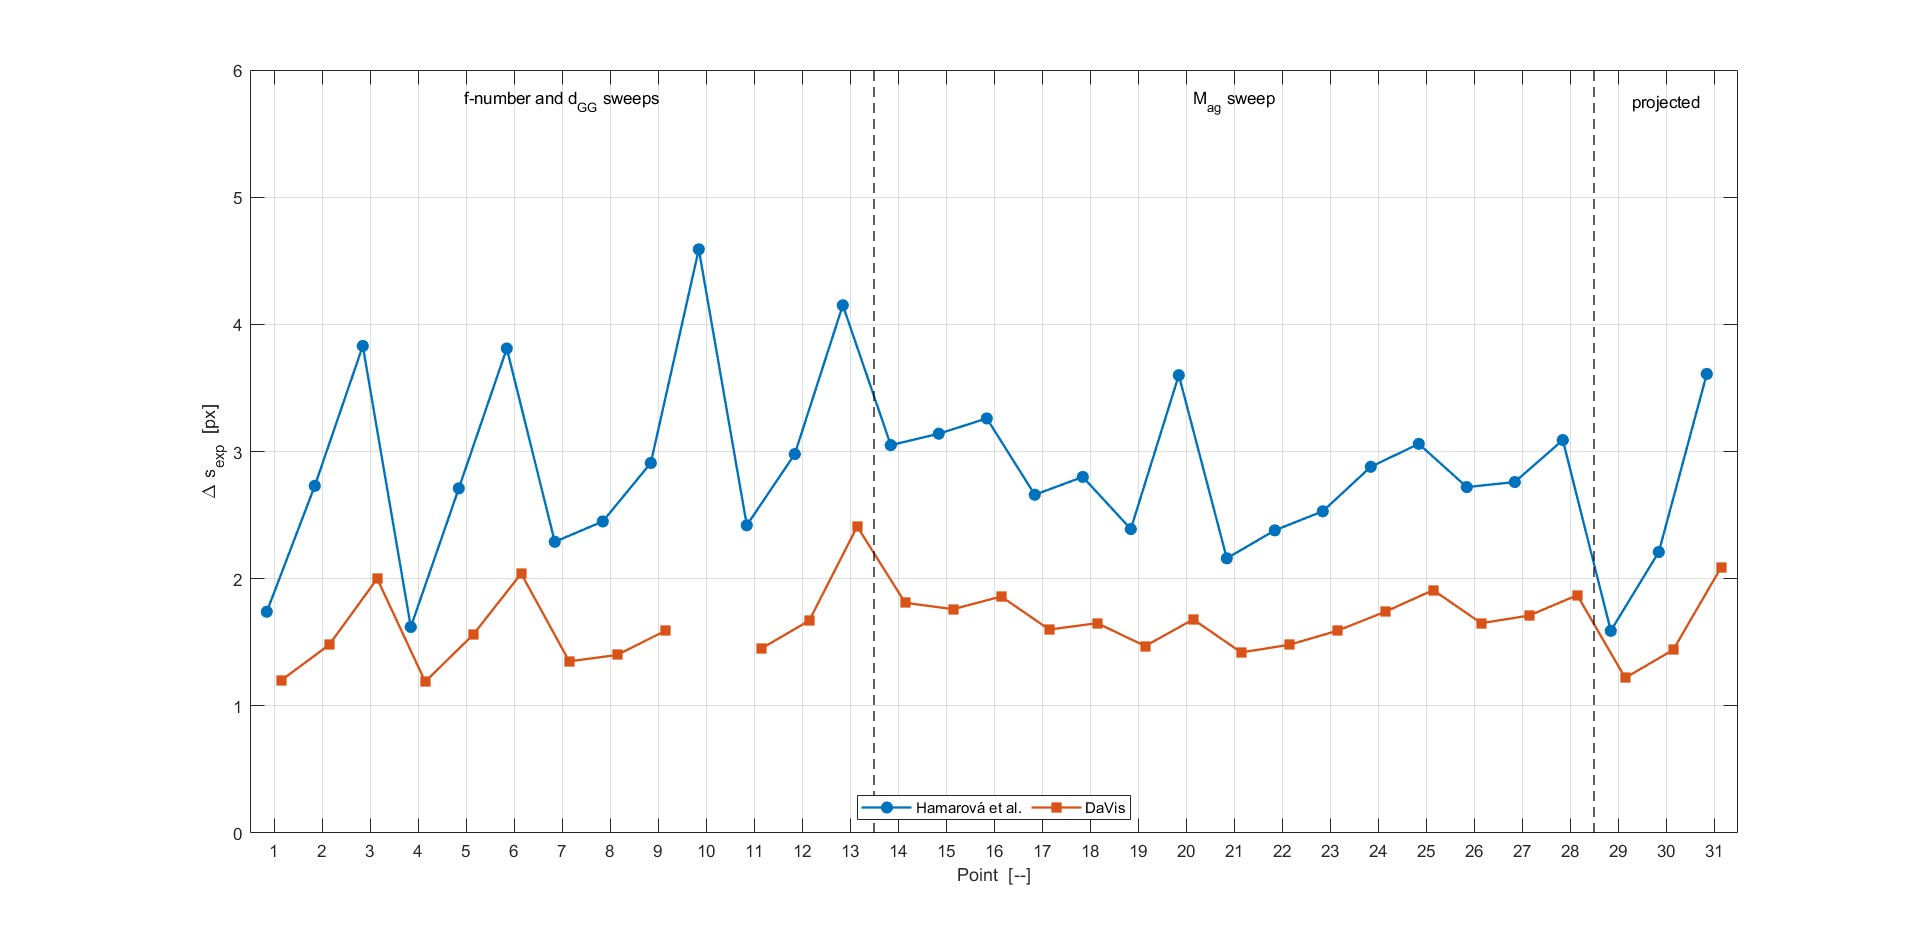
\includegraphics[width=\textwidth]{figures/speckle size per point.jpg}
    \caption{Average speckle size of every point of Table \ref{tab: speckle results}, computed with the autocorrelation method of Hamarová et al. \cite{Hamarova2016} and with the DaVis function. The dashed lines separate the $f_\#$ and $d_{GG}$ sweeps, the magnification sweep and the projected speckle points. DaVis returned no value for point 10}
    \label{fig: speckle size per point}
\end{figure}

% REVIEW: the deviations are in px while u_tot is in percent, so "vastly surpasses" compares different units, and it does not hold at every point (point 25: 0.06 px on 3.00 px is 2 percent, below u_tot = 3.42 percent). The magnification uncertainty "within 5% for a 10% deviation" has no budget in the thesis.
Regarding the Rayleigh limit reproduction, it is possible to see that the results are much more similar to the predicted values in order of magnitude if compared to the ones presented previously in Table \ref{tab: angled glass speckle results}. The deviations now span from 0.06 px to a maximum of 2.88 px, instead of 9.59 to 22.30 px from before. Nevertheless, the relative error is still large overall, with the worst results at the points with subpixel speckles and close to 5 px. The error also vastly surpasses the uncertainty associated with magnification, which stayed within 5\% for a 10\% deviation in $M_{ag}$, and post-processing, which had a maximum of 11.45\%. Regardless, the data obtained provides a better fit to the Rayleigh diffraction prediction, showing that the equation can be used as a rough preliminary estimator of the speckle size. The results also allow for the identification of useful trends and comparisons in speckle production, as will be shown.

% REVIEW: "direct speckles provide more intensity, which allows for lower exposures" is not supported by data in this chapter. Add a measurement or a citation.
Points 29 to 31 of Table \ref{tab: speckle results} were obtained with projected speckles. Compared to direct speckles, the projected speckles show a similar deviation to theory and an overall smaller speckle size, which is hinted by Figure \ref{fig: speckle f-number sweep}. The results are too similar to the direct speckle approach to discriminate which method to use based on speckle size. Therefore, the trade-off on how to create the speckle pattern depends more on practical considerations than on its speckle characteristics. Projected speckles might be preferable in applications where only one optical access is available; where powerful lasers are being used that could damage the camera or when the double-pass method of Meier \& Rösgen \cite{Meier&Roesgen2013} needs to be used for increased sensitivity. Direct speckles, on the other hand, provide more intensity, which allows for lower exposures, and might be preferable when a see-through optical access is available. 

%However, it might be more vulnerable to vibrations and decorrelation \cite{Buhlmann2020}, specially in cases where the background is very close to the test-section.

% The vulnerability to decorrelation mentioned in chapter 3 doesn't seem to be an exclusive issue to projected speckle but transversal to both configurations. It is caused when the diffusor is submitted to some degree of motion or vibration, specially when positioned very close to the test section. 

% REVIEW: the text and Table 6.8 describe the budget differently. Half-width: the standard deviation that minimizes the tail beyond 60 px (text) vs the range of widths within the noise floor (caption). Estimator term: the 1.5 percent reported by Hamarova (text) vs the spread between three estimators (caption). "As a consequence" does not follow from the previous sentence.
To better judge the deviation of the experiment, an uncertainty budget was constructed to compute the total uncertainties. They are displayed for each experimental point in Table \ref{tab: speckle results}. This total uncertainty corresponds to the ones obtained for the implementation of Hamarová et al.'s method and is reported in Table \ref{tab: speckle size uncertainty}. In their paper, the researchers reported an uncertainty of 1.5\% associated with their estimator. As a consequence, the budget is dominated by the Gaussian filter implemented. The Gaussian standard deviation was taken as a parameter and varied such that the tail of the autocorrelation function result after 60 px was minimized. The half-width of the method is, therefore, the achieved standard deviation and its individual uncertainty, assuming a rectangular distribution, is $u = a / \sqrt{3}$. The contribution is $u$ times the sensitivity coefficient. In the last row, the combined figure of the post-processing uncertainty can be found.

\begin{table}[htbp]
    \centering
    \caption{Uncertainty budget for the average speckle size obtained by the autocorrelation method. The flattening filter width is not measured with an instrument; it is selected by driving the tail of the autocorrelation to zero, so its half-width $a$ is the range of widths for which that tail remains within its noise floor, taken as $1/\sqrt{N_s}$ for a frame holding $N_s$ speckles. As in Table \ref{tab: angled glass uncertainty}, the width is treated as a rectangular distribution so that $u = a/\sqrt{3}$ \cite{JCGM2008}, and the contribution $c_\sigma$ is the sensitivity $\partial \Delta s_{exp} / \partial \sigma$, obtained by re-evaluating the speckle size one pixel either side of the selected width, multiplied by $u$. The estimator contribution is the spread between the two-dimensional, the average one-dimensional and the long vector estimators reported by Hamarová et al. \cite{Hamarova2016}. Both terms vary per point, so their range over the 31 points is given here and the totals are listed per point in Table \ref{tab: speckle results}.}
    \label{tab: speckle size uncertainty}
    \begin{tabular}{llrrr}
        \toprule
        Source & Instrument & $a$ & $u$ & Contribution $c_i$ [\%] \\
        \midrule
        Filter width $\sigma$      & Tail criterion & 2.0--67.0 px & 1.2--38.7 px & 0.06--11.36 \\
        Estimator choice           & Literature     & --           & 1.5 \%       & 1.50 \\
        \midrule
        Combined, $u_{\Delta s} = \sqrt{c_\sigma^2 + c_{est}^2}$ &  &  &  & 1.50--11.45 \\
        \bottomrule
    \end{tabular}
\end{table}

%Maybe this paragraph could be split into mag, aperture, d_GG and projected
% REVIEW: long paragraph, consider splitting it into aperture, magnification, d_GG and projected speckles. The magnification insensitivity found here is the opposite of Section 6.1 and needs to be reconciled.
Now that the error and uncertainties of the results have been discussed, the data can be plotted to better understand its behavior, such as f-stop dependency. The various $f_\#$ sweeps made during the experimental campaign allow the evaluation of whether the interference waves became diffraction limited at the pupil. Figure \ref{fig: speckle f-number sweep} shows the trend of average speckle size with f-stop number for four different configurations. All lines follow the characteristic increasing trend of a developed subjective speckle, which follows Equation \ref{equation: Rayleigh Limit}, and signals that the interference front is becoming diffraction limited at the lens pupil \cite{Goodman2020}. The red and yellow lines both share the same $d_{GG}$, which makes them viable for direct comparison. It appears that the increased magnification of the red line caused practically no effect in the average speckle size, displaying almost the same values as the yellow line. The same insensitivity to magnification was also experienced through points 14--28 shown in Figure \ref{fig: speckle magnification sweep}. Looking at the purple line compared to the latter two, it appears that the different $d_{GG}$ introduced some difference in the speckle size, with the purple exceeding the red by 0.68, 0.25 and 0.32 px for $f_\#$ = 4, 11.31 and 22.63, respectively, although the difference is only subpixel. In green, the projected speckle trend can also be analyzed, and it demonstrates that projected speckles are generally smaller, presenting smaller speckles even than the yellow line, which has a lower magnification than green. The figure shows some promising trends as there is a clear dependence on $f_\#$ and it indicates a tendency of projected speckles to be smaller than direct ones. However, it also shows an insensitivity to the optical magnification, contradicting Equation \ref{equation: Rayleigh Limit}, and the effect of $d_{GG}$ which will be further discussed next.

\begin{figure}[htbp]
    \centering
    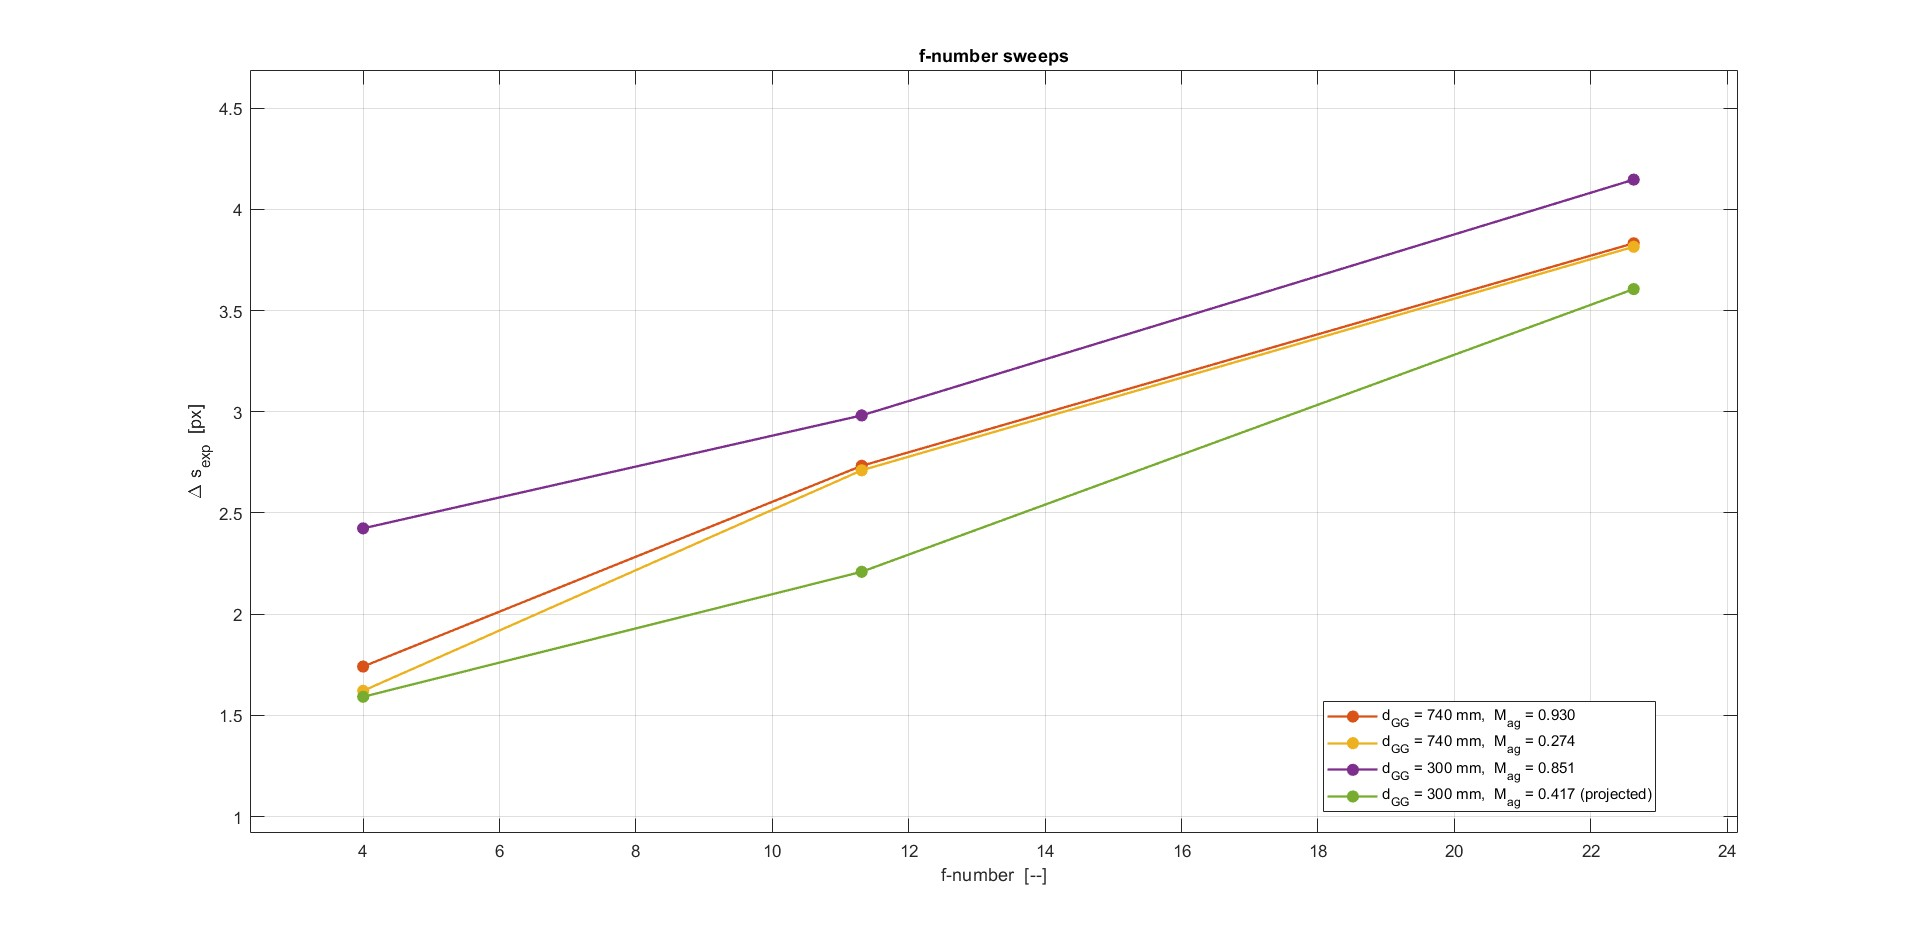
\includegraphics[width=\textwidth]{figures/speckle exp f-number sweep.jpg}
    \caption{Average speckle size versus f-stop number for the four aperture sweeps of the speckle investigation campaign. The red and yellow lines correspond to points 1--3 and 4--6, which share $d_{GG} = 740$ mm at two different magnifications. The purple line corresponds to points 11--13, acquired at $d_{GG} = 300$ mm, and the green line to points 29--31, obtained with projected speckles at the same $d_{GG}$}
    \label{fig: speckle f-number sweep}
\end{figure}


% REVIEW: "beam ratio of 0.25" is not defined. The literature argument is from silence ("does not mention the effect"). The final recommendation generalizes from five points at one f# and one M_ag. The mechanism should match the one used in Section 6.1.
Since the beam was expanded through a convergent lens, the distance between that lens and the ground glass diffuser is a proxy for the beam diameter, therefore, it is possible to verify the influence of the beam diameter in the speckle generation by plotting the points where only $d_{GG}$ was varied. Figure \ref{fig: speckle dGG sweep} shows that the average speckle size remains consistent for high $d_{GG}$, as it varies from 2.91 px at 190 mm, dips to 2.29 px at 450 mm and goes to 2.71 px at 740 mm. This variation is consistent with the findings of Figure \ref{fig: speckle f-number sweep}. It demonstrates that $d_{GG}$ can increase the speckle size but for large distances the spread is practically subpixel. However, the figure also shows a spike at low $d_{GG}$ when the beam diameter is small, reaching 4.59 px at 100 mm with beam ratio of 0.25. The DaVis function failed to compute a value for this point, as the illuminated envelope was too small and the speckles too large. The effect can be better visualized through Figure \ref{fig: speckle patterns dGG} which displays side-by-side the captured speckle patterns for points 5, 8 and 10 respectively. This data supports the hypothesis that the larger speckle size in the angled glass experiment was caused by the small diameter of the laser when it hit the 1.27 cm ground glass diffuser. The fact that the speckle size changed less for larger distances is also backed up by the literature, which does not mention the effect of the laser diameter in the speckle generation. In addition, it means that, when designing the laser optical setup, an experimentalist must only worry about expanding the laser beam to fill the desired field of view.

\begin{figure}[htbp]
    \centering
    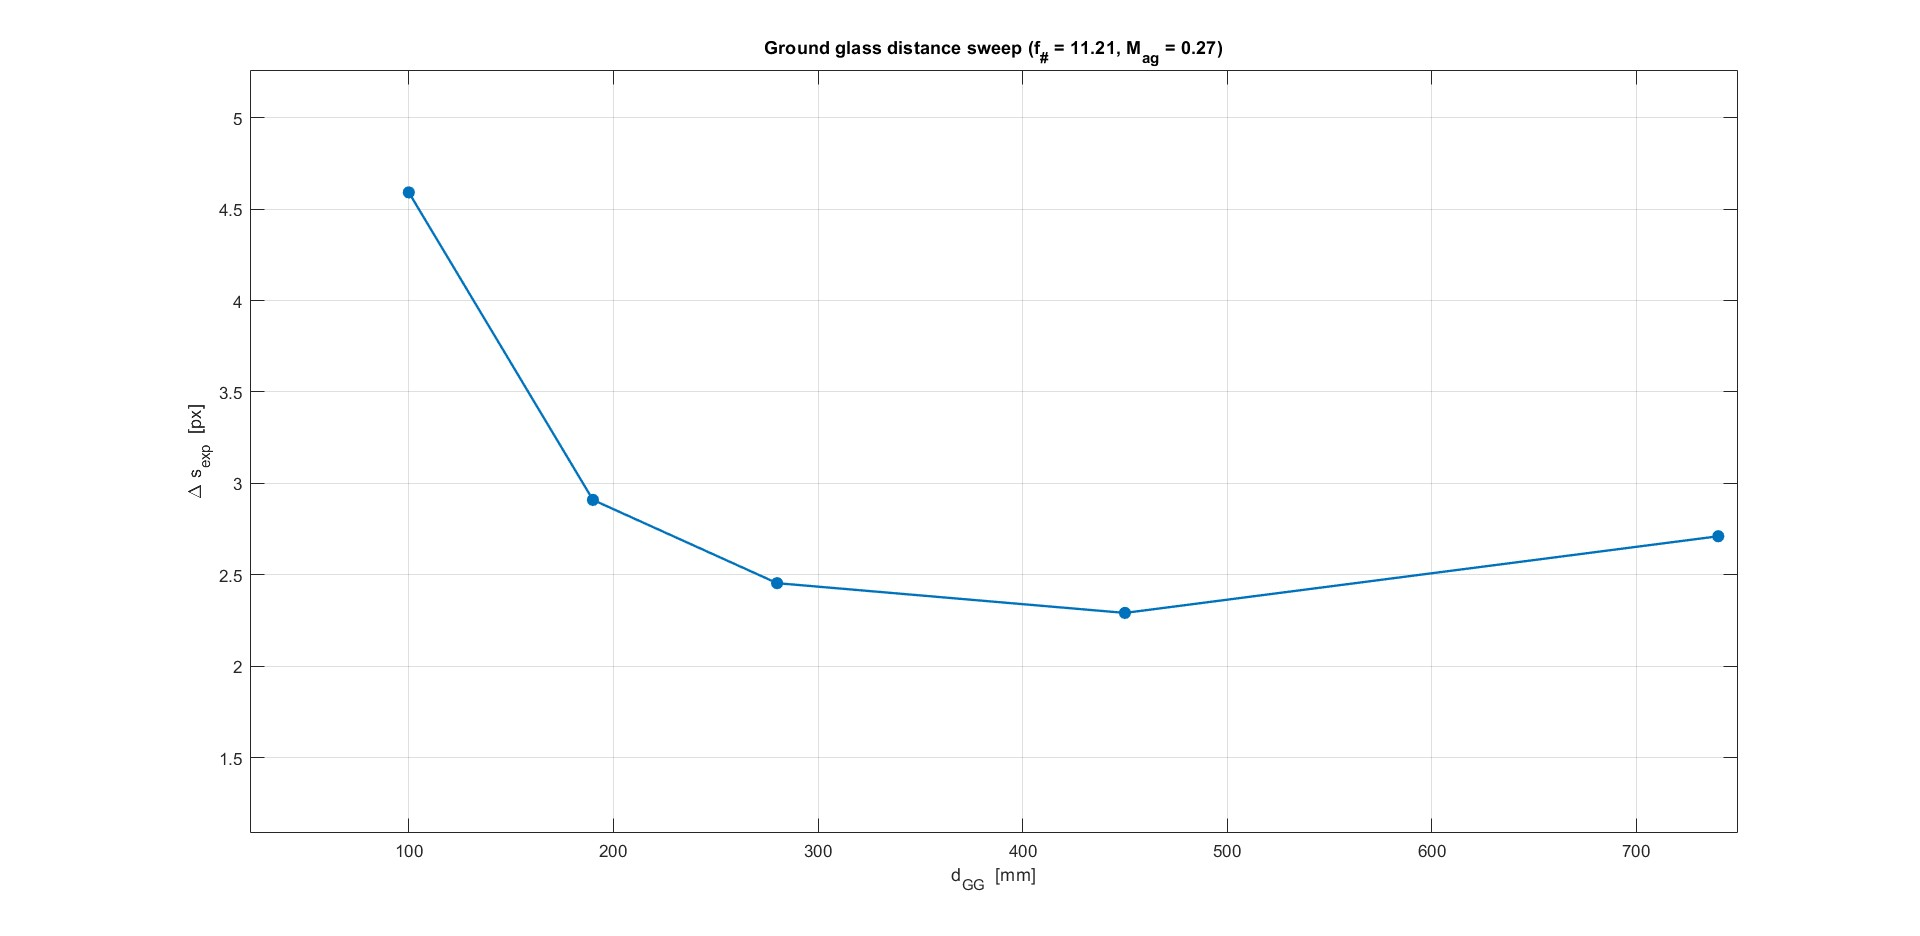
\includegraphics[width=\textwidth]{figures/Speckle d_GG Sweep.jpg}
    \caption{Average speckle size versus the distance between the beam expander lens and the ground glass diffuser, for points 5 and 7--10 of Table \ref{tab: speckle results}, all acquired at $f_\# = 11.31$ and $M_{ag_{exp}} = 0.296$}
    \label{fig: speckle dGG sweep}
\end{figure}

\begin{figure}[htbp]
    \centering
    \begin{subfigure}[b]{0.32\textwidth}
        \centering
        
\includegraphics[width=\textwidth]{figures/Speckle pattern point 5.jpg}
        \caption{Point 5, $d_{GG} = 740$ mm}
        \label{fig: speckle pattern point 5}
    \end{subfigure}
    \hfill
    \begin{subfigure}[b]{0.32\textwidth}
        \centering
        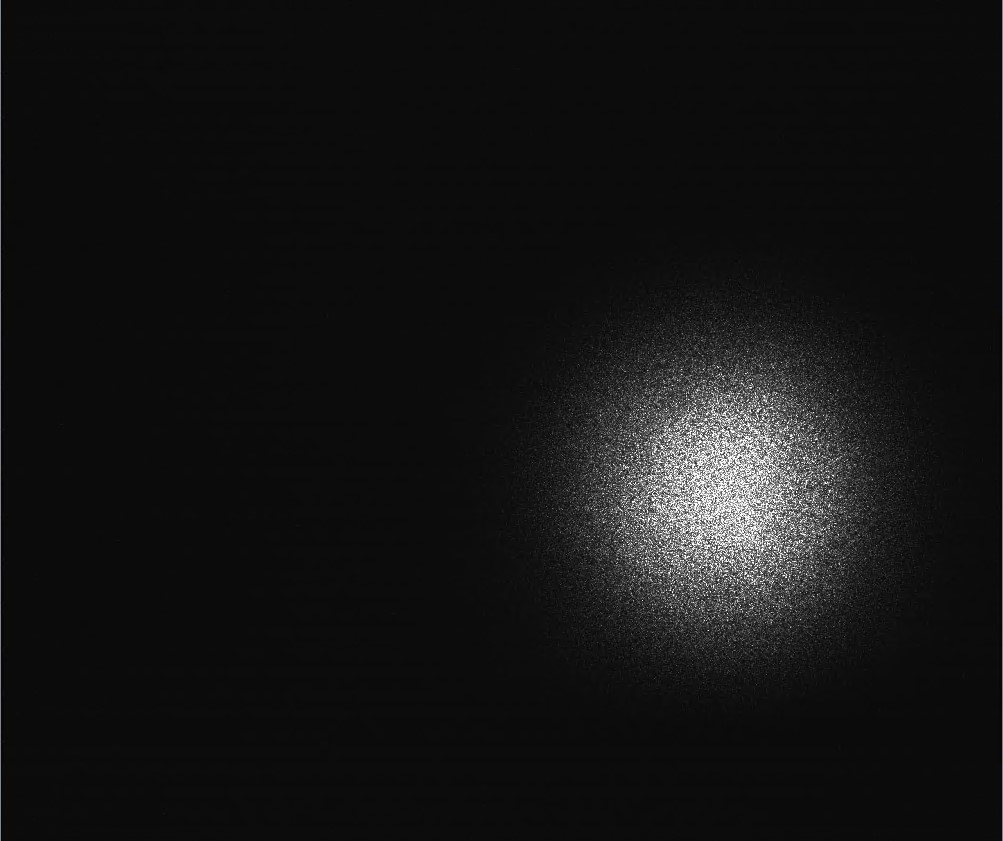
\includegraphics[width=\textwidth]{figures/Speckle pattern point 8.jpg}
        \caption{Point 8, $d_{GG} = 280$ mm}
        \label{fig: speckle pattern point 8}
    \end{subfigure}
    \hfill
    \begin{subfigure}[b]{0.32\textwidth}
        \centering
        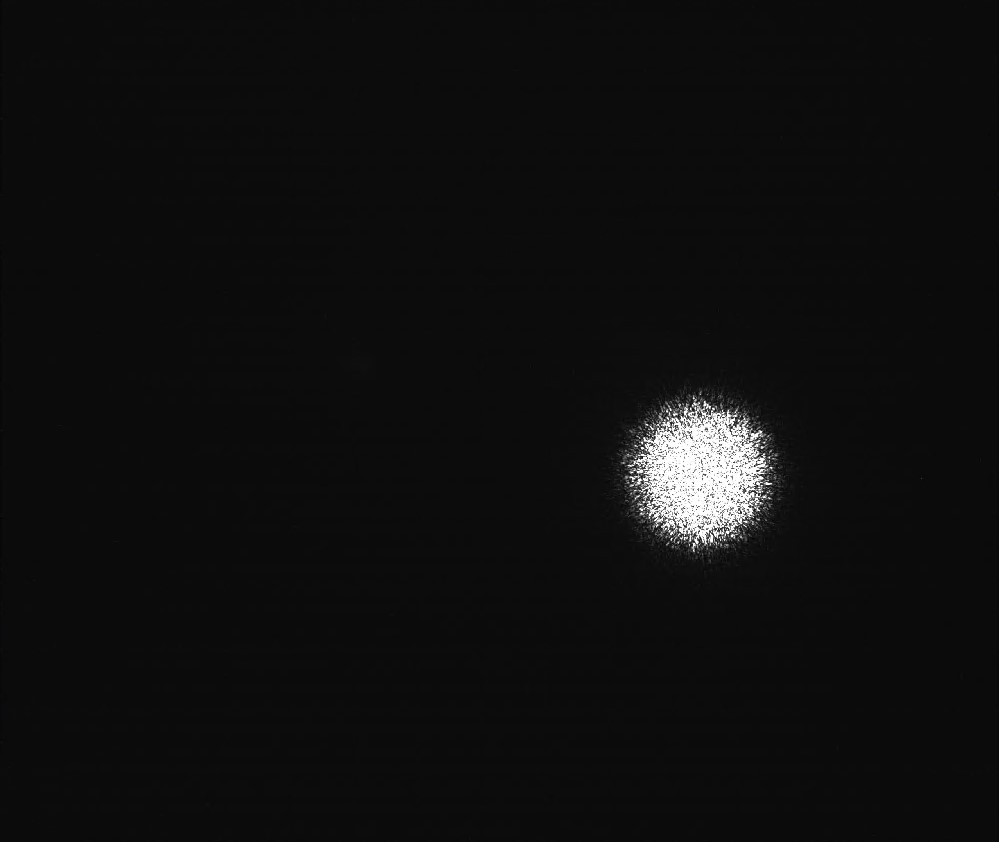
\includegraphics[width=\textwidth]{figures/Speckle pattern point 10.jpg}
        \caption{Point 10, $d_{GG} = 100$ mm}
        \label{fig: speckle pattern point 10}
    \end{subfigure}
    \caption{Raw speckle patterns captured at $f_\# = 11.31$ and $M_{ag_{exp}} = 0.296$ for three distances between the beam expander lens and the ground glass diffuser. As $d_{GG}$ decreases, the illuminated area on the diffuser shrinks and the speckle pattern contracts from filling the sensor to a small bright spot}
    \label{fig: speckle patterns dGG}
\end{figure}


To better assess the effect of optical magnification in the speckle generation process, a sweep of the focal distance was conducted through points 14--28 and is shown in Figure \ref{fig: speckle magnification sweep}. It is worth mentioning that the magnification value of these points is less accurate than the others, as the focal distance was obtained through the distance marks of the camera lens. Nevertheless, the figure shows, for a different $d_{GG}$, the same speckle size insensitivity to optical magnification that was identified in Figure \ref{fig: speckle f-number sweep}. That effectively contradicts the Rayleigh diffraction limit equation and reduces the number of control variables an experimentalist would have when designing the experimental setup.

\begin{figure}[htbp]
    \centering
    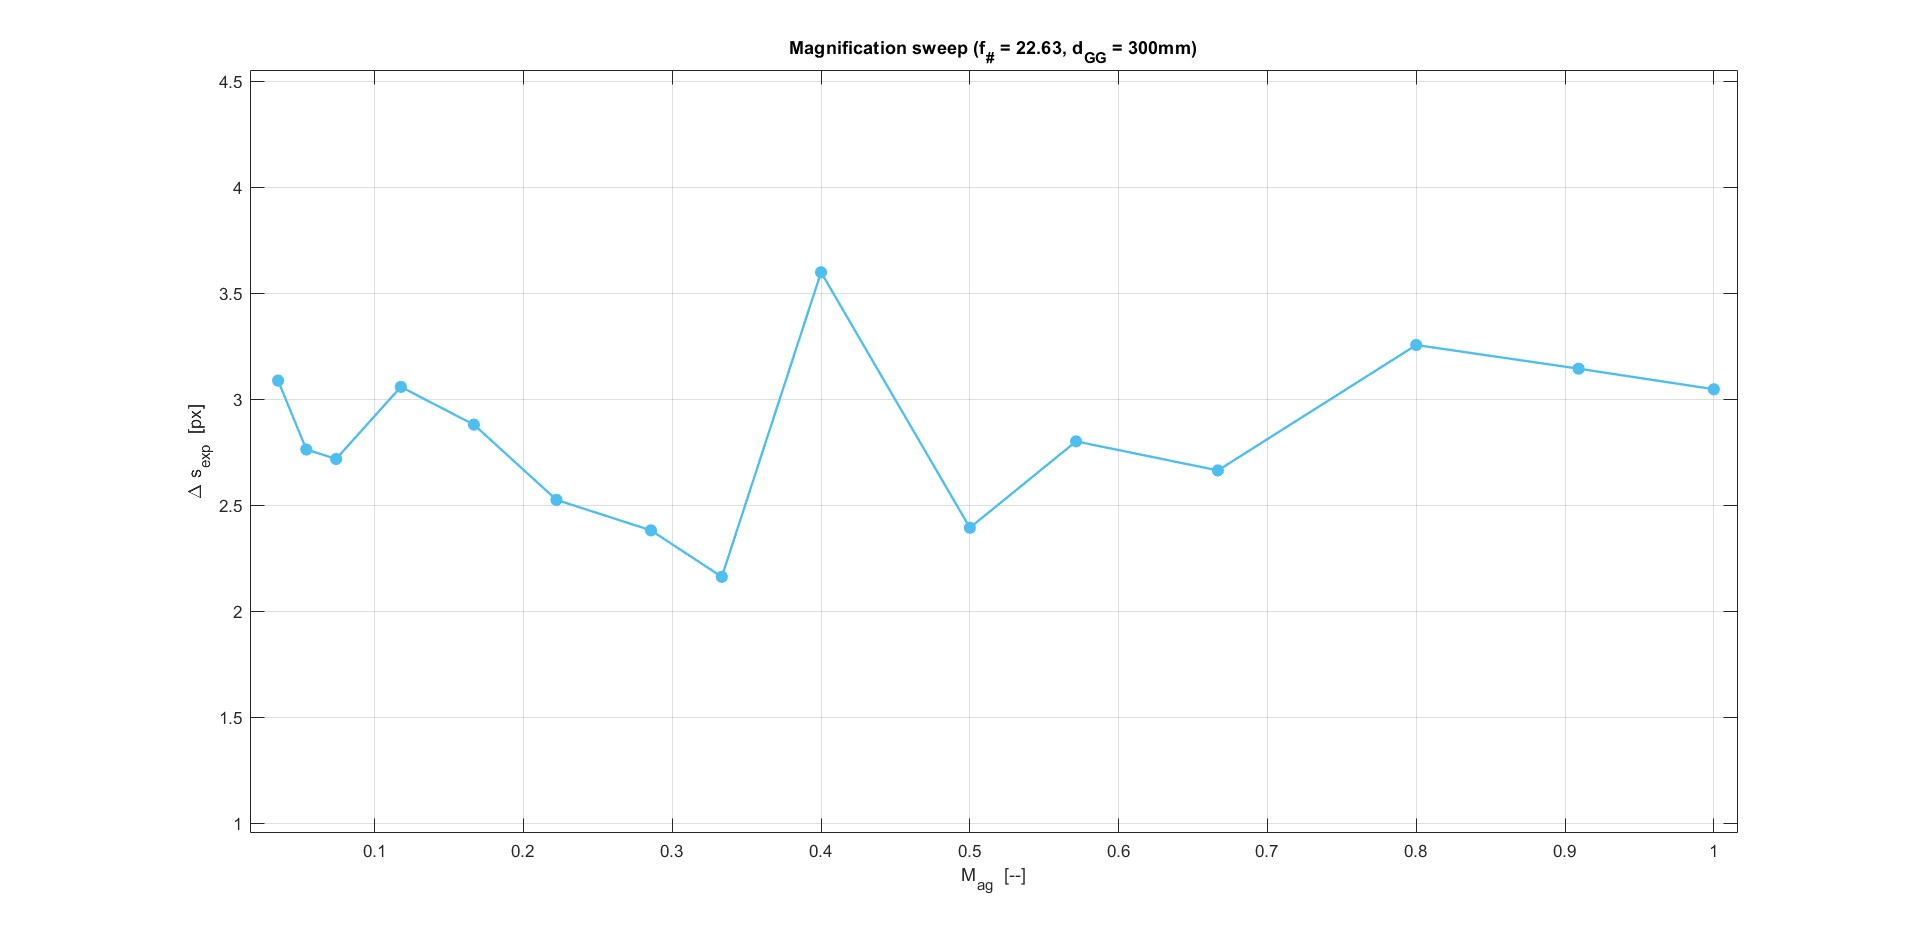
\includegraphics[width=\textwidth]{figures/speckle exp mag sweep.jpg}
    \caption{Average speckle size versus optical magnification for points 14--28 of Table \ref{tab: speckle results}, acquired at a fixed $f_\# = 22.63$ and $d_{GG} = 300$ mm. The magnification of these points was obtained from the distance marks of the camera lens rather than with the calibration plate}
    \label{fig: speckle magnification sweep}
\end{figure}

The speckle pattern investigation campaign allowed for the study of the speckle generation process. It successfully reproduced finer speckles than the angled glass experiment, showed the dependence of the speckle size on the f-stop number, investigated the effect of a small incidence beam in the diffuser and compared direct with projected speckle. However, the data showed unexpected insensitivity to magnification variations and still deviated significantly from the speckle predicted through the Rayleigh limit. It is worth reiterating that the speckle generation process is a complex intrinsically random phenomenon and to treat it with much more detail would be out of the scope of this thesis. For now, the data at hand make it possible to define a laser speckle generator capable of producing speckles within the 2--5 pixel range. Therefore, the findings of this campaign are enough to proceed to the correct application of Laser Speckled BOS to image a real schlieren object, in this case a compressible jet.


\section{Compressible Jet Experiment Results}
\label{section: Compressible Jet Experiment Results}

% REVIEW: NPR_g in the subfigure captions of the next figure is not defined anywhere. This introduction also promises a quantitative density field, but that subsection is still empty.
An underexpanded compressible jet was chosen as the object of study for the implementation of SBOS to a real schlieren object. The goal of this experiment was to image the jet at various nozzle pressure ratios ($NPR$), post-process the raw displacement data into a quantitative density field, analyze the jet structure and study the influence of an increase in nozzle pressure. The setup of this experiment was explained in Section \ref{section: Compressible jet experiment}. Figure \ref{fig: compressible jet displacement fields} displays the results of the cross correlation for the 6 different gauge pressures set at the wall air tap.

\begin{figure}[htbp]
    \centering
    \begin{subfigure}[b]{0.32\textwidth}
        \centering
        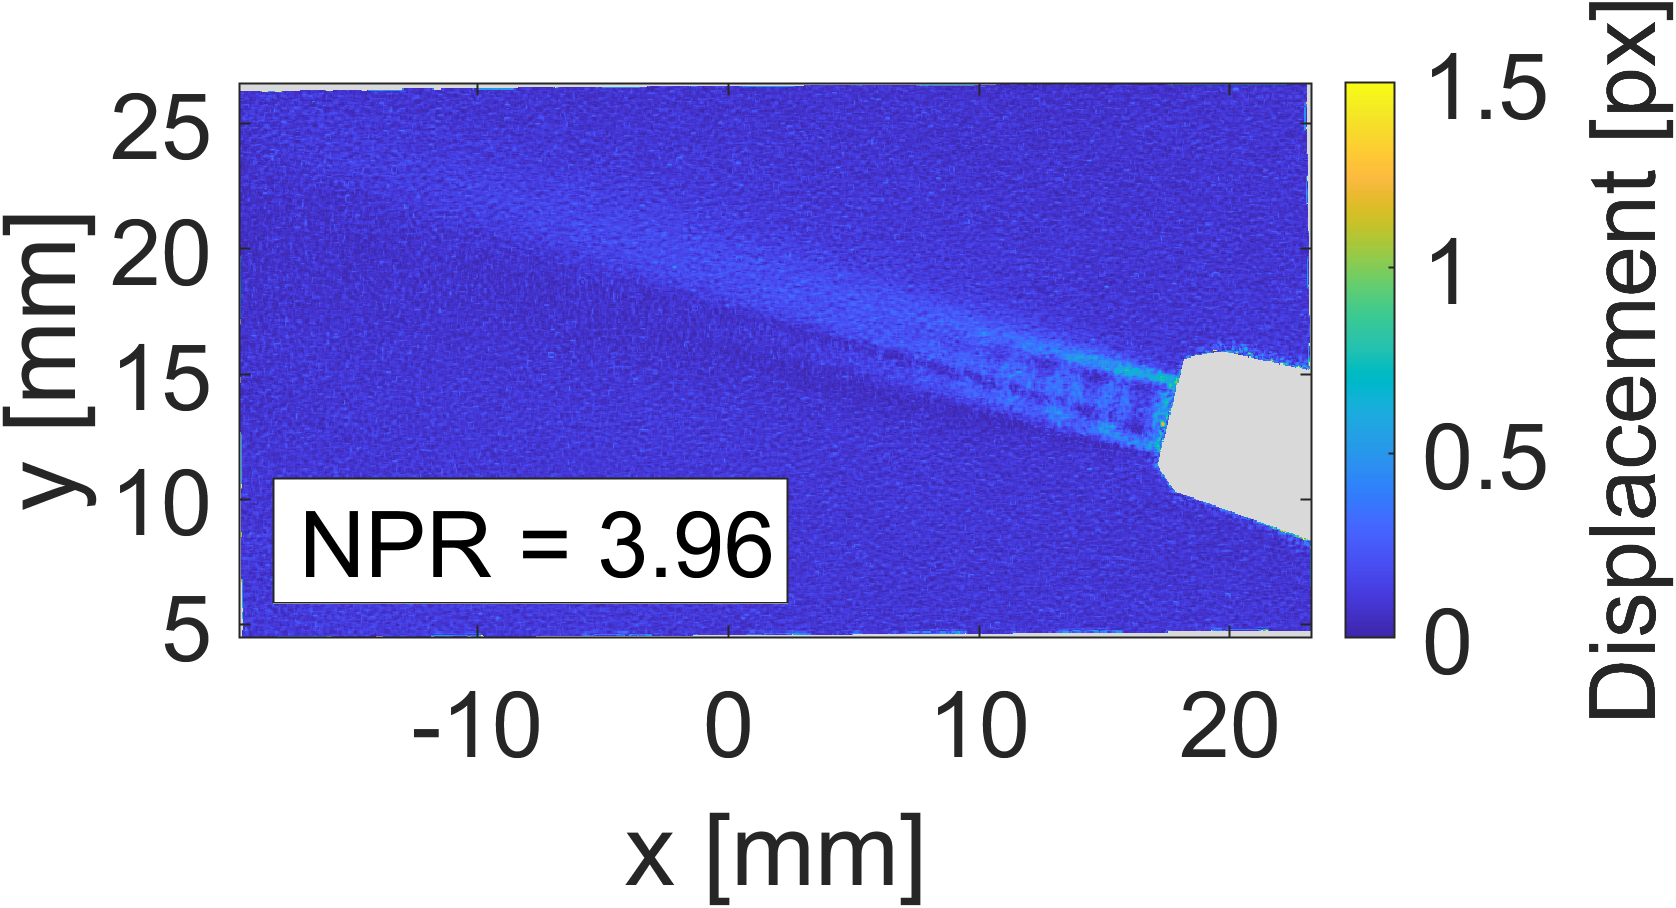
\includegraphics[width=\textwidth]{figures/jet displacement 3bar.png}
        \caption{$p_g = 3$ bar, with respective $NPR_g = 3.96$}
        \label{fig: jet displacement 3bar}
    \end{subfigure}
    \hfill
    \begin{subfigure}[b]{0.32\textwidth}
        \centering
        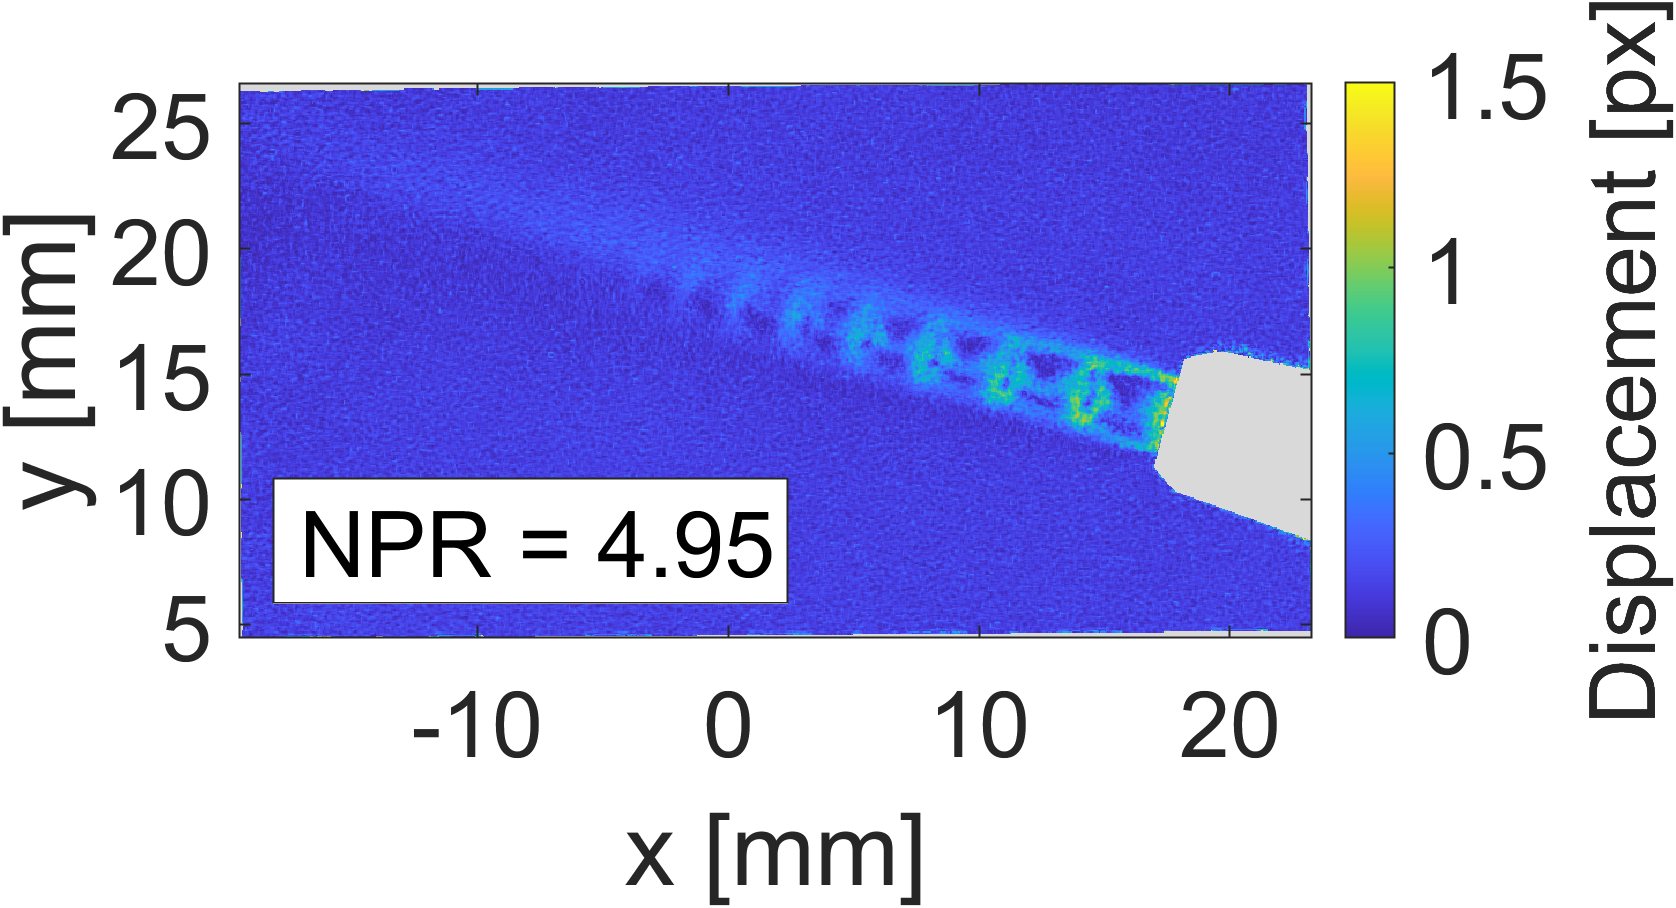
\includegraphics[width=\textwidth]{figures/jet displacement 4bar.png}
        \caption{$p_g = 4$ bar, with respective $NPR_g = 4.95$}
        \label{fig: jet displacement 4bar}
    \end{subfigure}
    \hfill
    \begin{subfigure}[b]{0.32\textwidth}
        \centering
        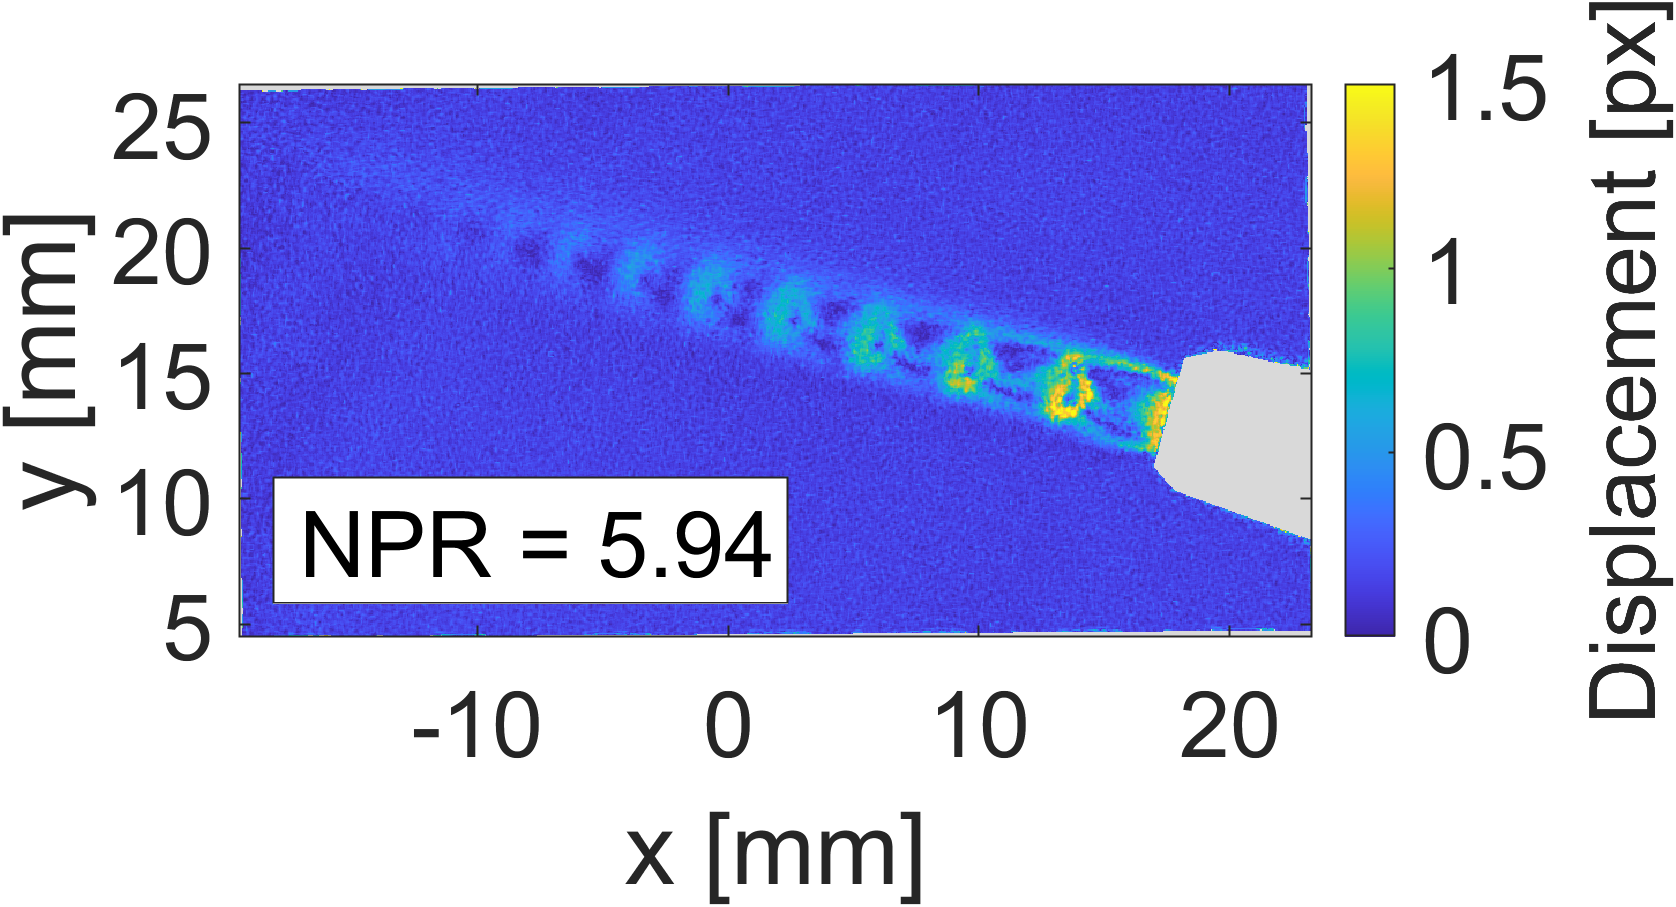
\includegraphics[width=\textwidth]{figures/jet displacement 5bar.png}
        \caption{$p_g = 5$ bar, with respective $NPR_g = 5.94$}
        \label{fig: jet displacement 5bar}
    \end{subfigure}

    \vspace{0.5em}

    \begin{subfigure}[b]{0.32\textwidth}
        \centering
        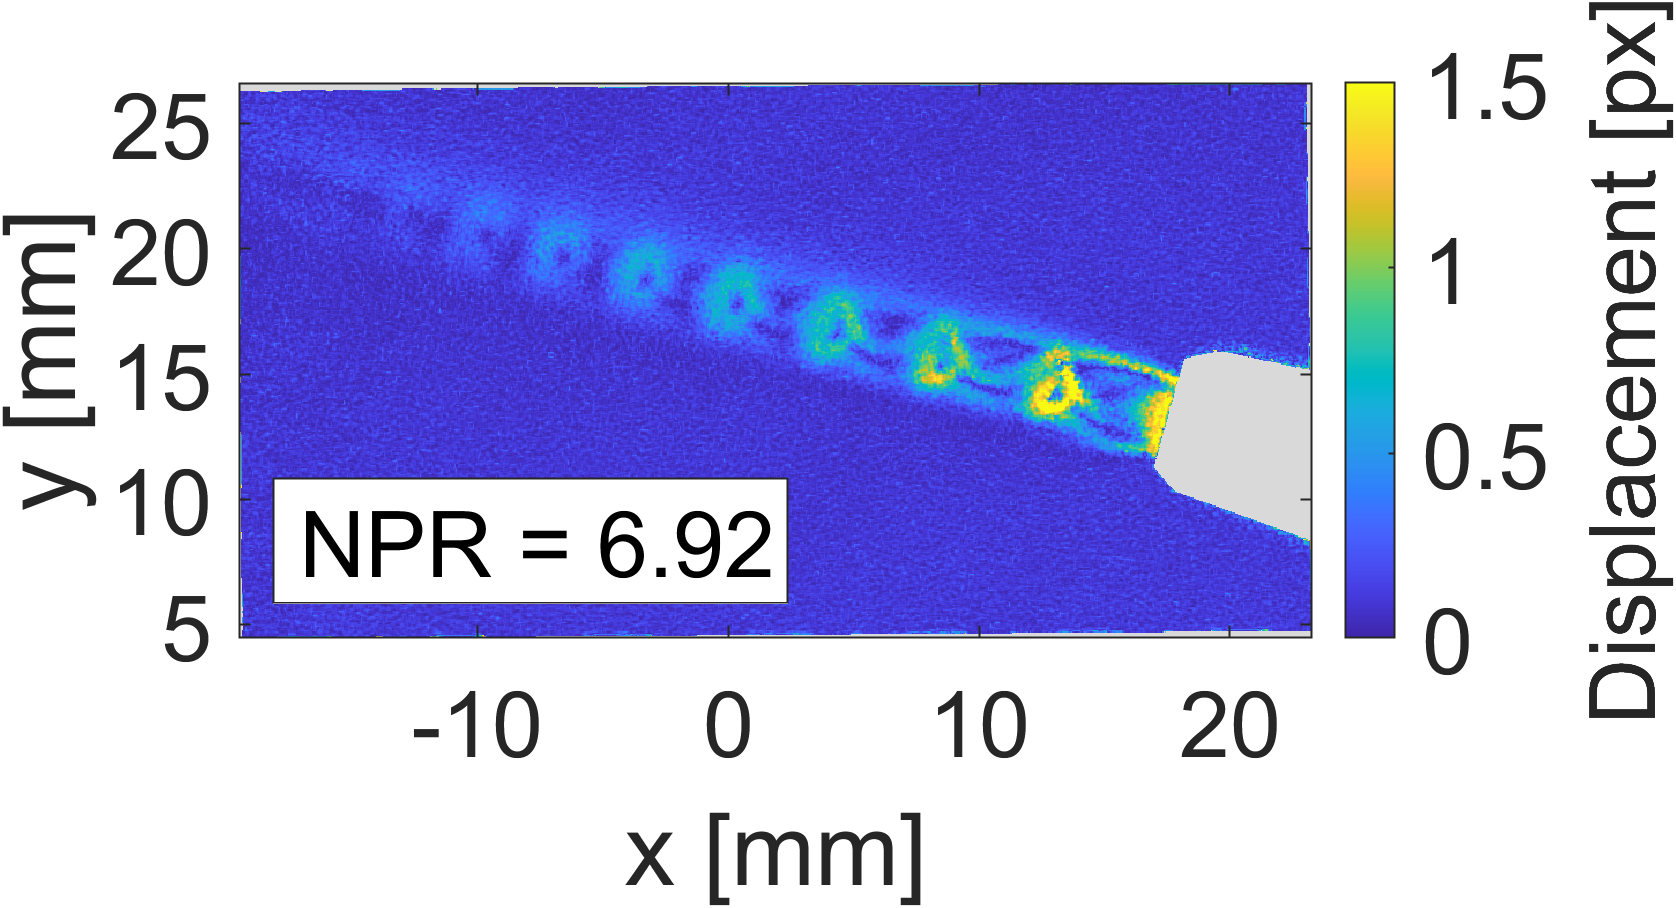
\includegraphics[width=\textwidth]{figures/jet displacement 6bar.png}
        \caption{$p_g = 6$ bar, with respective $NPR_g = 6.92$}
        \label{fig: jet displacement 6bar}
    \end{subfigure}
    \hfill
    \begin{subfigure}[b]{0.32\textwidth}
        \centering
        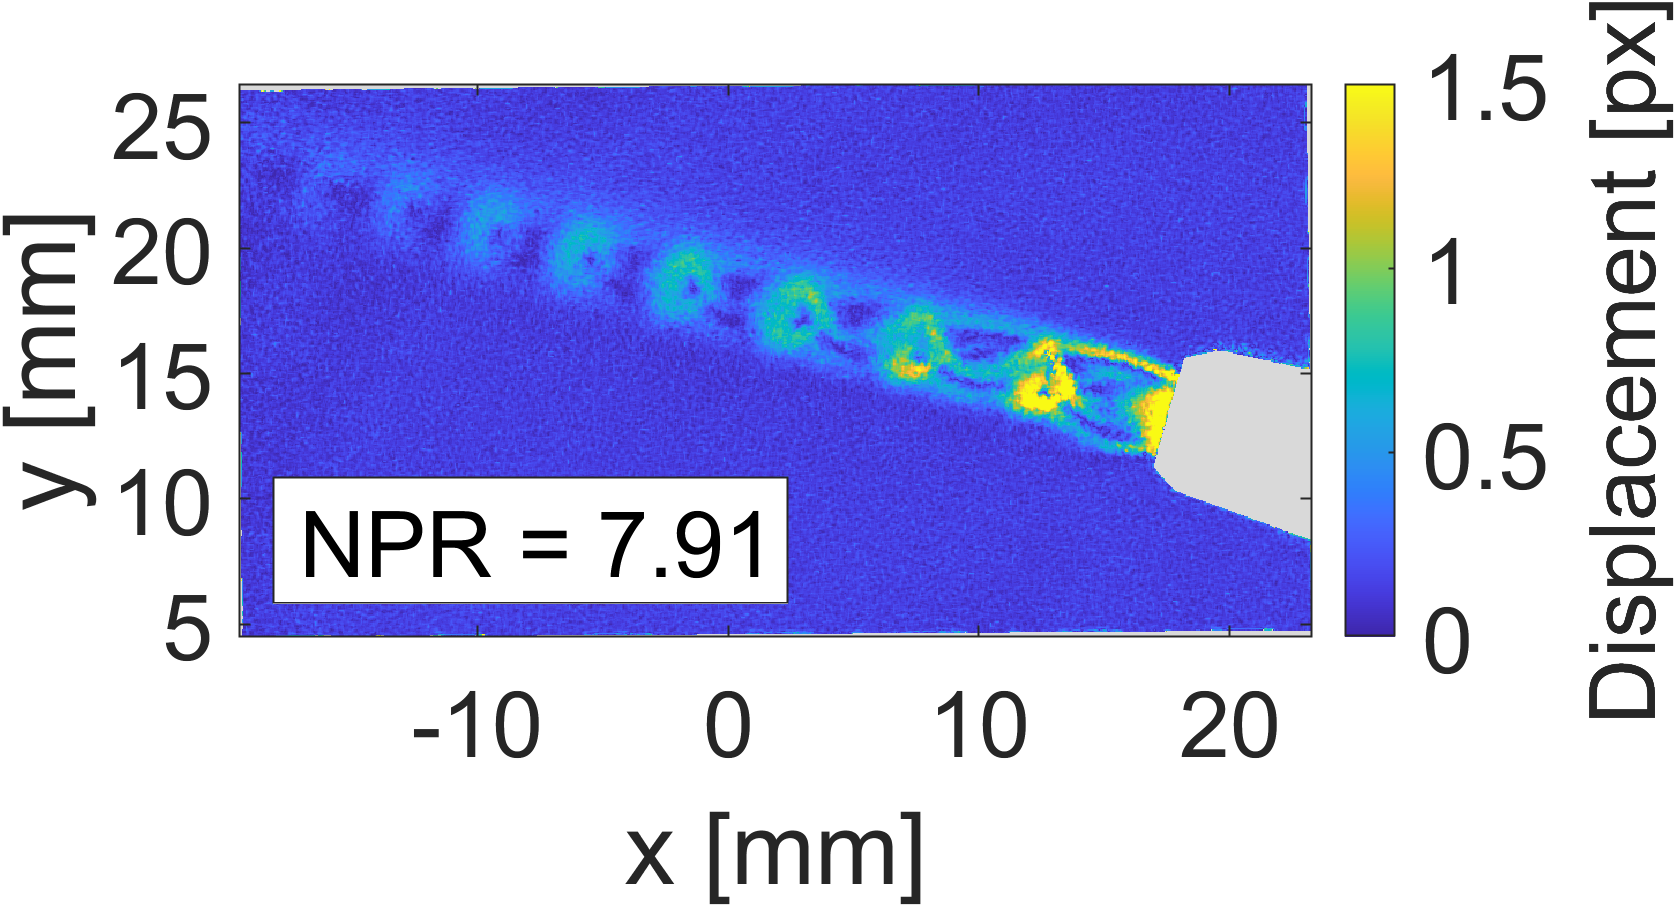
\includegraphics[width=\textwidth]{figures/jet displacement 7bar.png}
        \caption{$p_g = 7$ bar, with respective $NPR_g = 7.91$}
        \label{fig: jet displacement 7bar}
    \end{subfigure}
    \hfill
    \begin{subfigure}[b]{0.32\textwidth}
        \centering
        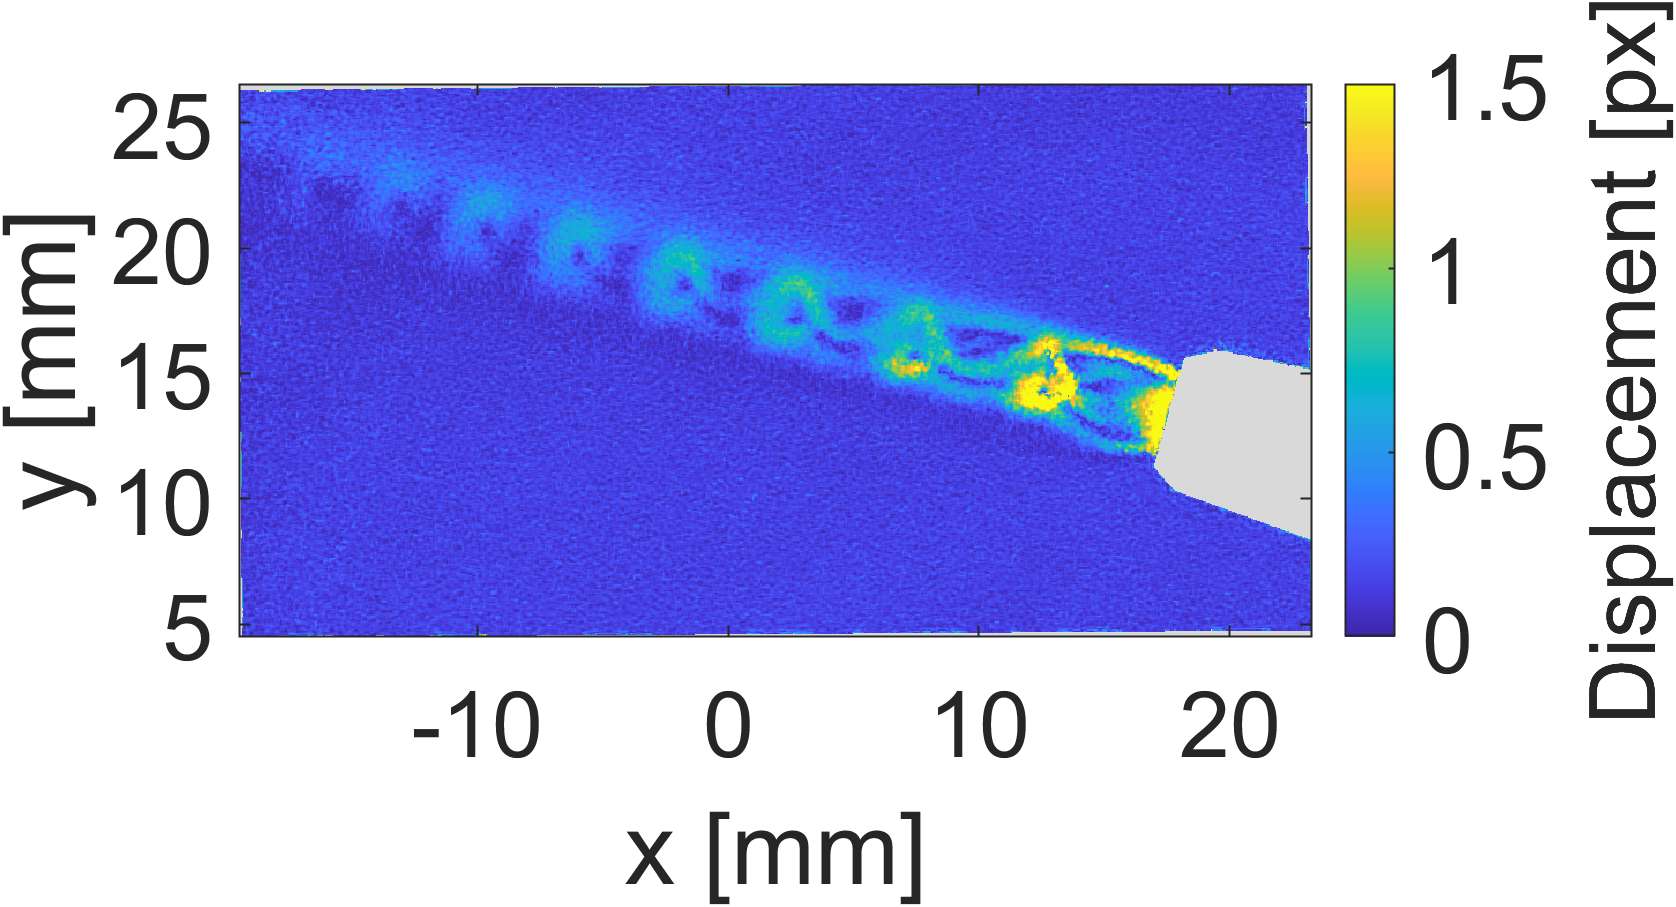
\includegraphics[width=\textwidth]{figures/jet displacement 8bar.png}
        \caption{$p_g = 8$ bar, with respective $NPR_g = 8.90$}
        \label{fig: jet displacement 8bar}
    \end{subfigure}
    \caption{SBOS results for a compressible jet. Displacement magnitude fields obtained through cross correlation for air tap gauge pressures from 3 bar to 8 bar with a step of 1 bar. All fields share the same color scale and masked vectors are shown in grey}
    \label{fig: compressible jet displacement fields}
\end{figure}

% REVIEW: the 7 and 8 bar cases have NPR_g = 7.91 and 8.90, above the 4 to 7 range, so they would fall in the single barrel regime.
Comparing the different images displayed by Figure \ref{fig: compressible jet displacement fields}, it is possible to assess the effect of different $NPR$ to the underexpanded jet structure. As explained in Section \ref{section: Compressible Jet Theory}, an increase in $NPR$ leads to an increase in shock cell length and a fundamental change in the jet structure at certain pressure ranges. Comparing the result for $p_g = 3$ bar to $p_g = 8$ bar, the shock cell length does indeed increase, together with the number of cells and a bigger bulge mid-cell. However, there is very little change in the shock cell length for gauge pressures 6 through 8 bar. Moreover, from Figure \ref{fig: jet displacement 4bar} onward the $NPR$ is within 4 to 7 so the formation of a Mach disk together with a "barrel" shaped shock cell would be expected, see Figure \ref{fig: highly underexpanded jet}. Nevertheless, all images seem to display an "X" shape, related to a nozzle pressure ratio of 2 to 4, Figure \ref{fig: moderately underexpanded jet}. Together, these deviations from theory indicate that the real pressure ratios at the nozzle are not what they would be if the total pressure were maintained from the wall air tap gauge, through the hose and out of the air gun. Therefore, there must be heavy pressure losses present throughout the line that need to be accounted for and new estimates of the nozzle pressure ratios must be computed.

% REVIEW: the text says p_e is obtained, but Table 6.9 reports p_0. The uncertainties are said to correspond to +1 deg in nu, but rows b to e use the -1 deg bound and row a the smaller bound. Row a rests on nu = 1 deg with a 1 deg reading uncertainty; consider commenting on that precision.
The strategy envisioned to better estimate the nozzle pressure ratio builds on top of the definition of the Prandtl-Meyer angle. As explained in Section \ref{section: Compressibility}, $\nu$ is the turning angle needed for a flow at a certain Mach number $M_1$ to expand to a Mach number $M_2$. In the case studied, the flow is choked at the nozzle exit, so the Mach number at the exit is assumed to be equal to one $M_e = 1$. At the lip, the flow expands isentropically until it reaches a certain $M_j$ at ambient pressure. Therefore, the angle of the flow at the shear layer is equal to $\varphi = \nu(M_j)$ relative to the jet axis. So, to better estimate the $NPR$, the images were then treated to make the jet axis horizontal, then the shear layer angle at the lip was measured, $M_j$ was calculated through the Prandtl-Meyer function and a value for $p_e$ was obtained using isentropic expansion. The values can be found in Table \ref{tab: compressible jet NPR estimates} together with the uncertainty corresponding to $+ 1^\circ$ in $\nu$.

\begin{table}[htbp]
    \centering
    \caption{Estimated jet conditions for each Prandtl-Meyer angle $\nu$. $M_j$ is the jet Mach number, $NPR$ the nozzle pressure ratio and $p_0$ the absolute total pressure. The uncertainties $u_{M_j}$, $u_{NPR}$ and $u_{p_0}$ are given relative to their respective values. The data is organized in letters from "a)" to "f)", corresponding to the order of the images in Figure \ref{fig: compressible jet displacement fields}}
    \label{tab: compressible jet NPR estimates}
    \begin{tabular}{lrrrrrrr}
        \toprule
        Data & $\nu$ & $M_j$ & $u_{M_j}$ & $NPR$ & $u_{NPR}$ & $p_0$ & $u_{p_0}$ \\
             & [$^{\circ}$] & [-] & [\%] & [-] & [\%] & [bar] & [\%] \\
        \midrule
        a) &  1 & 1.082 & 4.71 & 2.088 & 6.51 & 2.115 & 6.52 \\
        b) &  3 & 1.177 & 3.74 & 2.353 & 5.48 & 2.384 & 5.49 \\
        c) &  5 & 1.257 & 3.10 & 2.613 & 5.17 & 2.647 & 5.14 \\
        d) &  8 & 1.366 & 2.64 & 3.032 & 5.01 & 3.072 & 5.01 \\
        e) & 10 & 1.435 & 2.44 & 3.344 & 5.02 & 3.387 & 5.02 \\
        f) & 13 & 1.537 & 2.21 & 3.875 & 5.08 & 3.925 & 5.10 \\
        \bottomrule
    \end{tabular}
\end{table}

% REVIEW: e to f is the largest NPR step in Table 6.9 (3.344 to 3.875), not a small one. L_s changes least there (4.95 to 5.00 mm), which is also where the Emden fit diverges.
The $NPR$ estimates displayed in Table \ref{tab: compressible jet NPR estimates} better fit the theory but also mean that the pressure losses in the line were extremely high. The nozzle pressure ratios range from 2 to 4, exactly the range where an "X" shaped shock cell would be expected. Moreover, the pressures of datasets e and f change very little between them, while there is a big difference between a and f, which is coherent with the similar pictures obtained. A question arises, however, when the estimate of total pressure is compared with the one at the air tap gauge, as loss of over 40\% cannot be explained with friction losses alone. These other sources of loss were probably choke points in the line, at quick disconnect joints or at a non-fully pressed air gun trigger. Another way to verify these estimates is by computing the density gradient field, measuring the shock cell length and relating them to the NPR through the relationships of Section \ref{section: Compressible Jet Theory}, this way validating it with literature data.

A density gradient field can be obtained assuming a planar field, through Equation \ref{equation: Displacement and Density Gradient}. This result corresponds to the projection of the axisymmetric body. In reality, the thickness of the object $W$ and the density gradient vary with the radius, so this solution will underestimate the density gradients at the borders of the jet. Nevertheless, it is useful to qualitatively study the shock cell structure, as the periodicity of the cell and the gradient signs are maintained in the projection. Figure \ref{fig: dataset f density gradients} shows the gradients for dataset f in the two directions s and n together with the magnitude of the vector. For this application, the background of the image was removed by calculating the median vector of a window only containing the background, then the image was rotated and translated such that the jet axis is horizontal and corresponds to n = 0.

\begin{figure}[htbp]
    \centering
    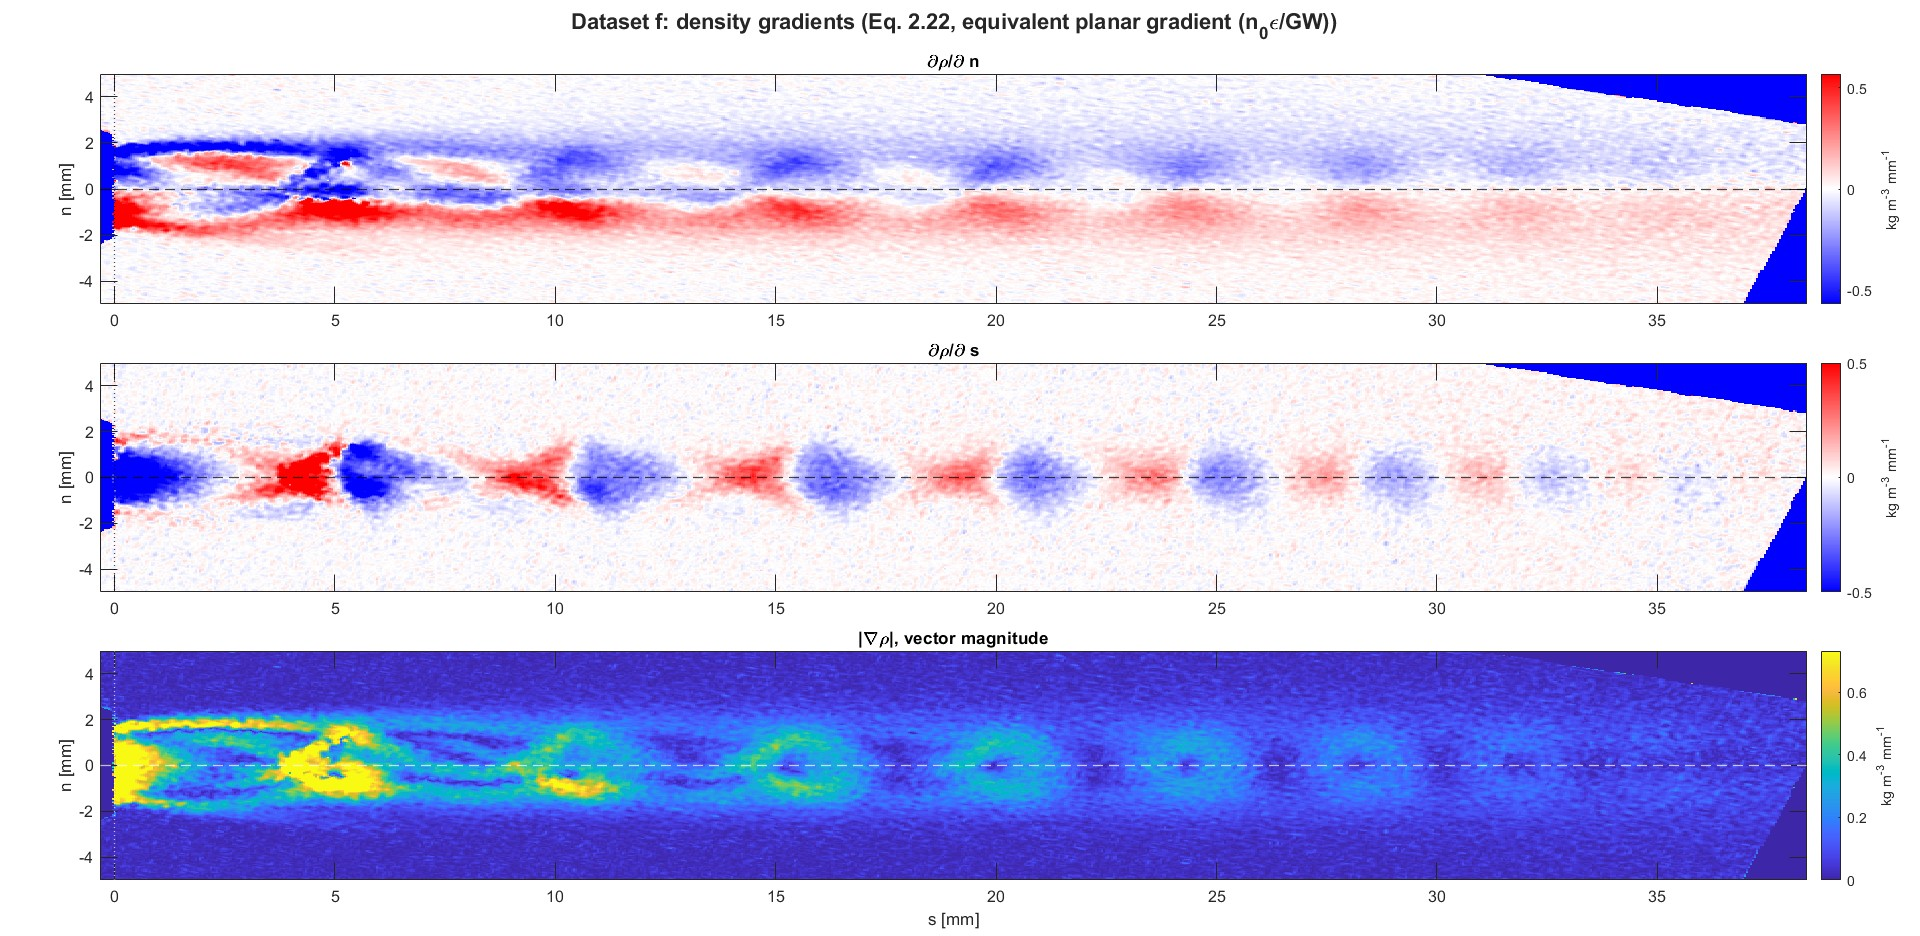
\includegraphics[width=\textwidth]{figures/Dataset f density gradients.jpg}
    \caption{Density gradient fields of dataset f obtained assuming a planar field. The top plot displays the density gradient in the n direction, the middle plot the density gradient in the s direction and the bottom plot the magnitude of the density gradient vector. The s axis is aligned with the jet axis with its origin at the nozzle exit, while n is normal to it}
    \label{fig: dataset f density gradients}
\end{figure}

Following the middle plot of Figure \ref{fig: dataset f density gradients}, correspondent to the density gradient in the s direction, the jet structures can be easily identified. Spanning from the lip to the axis at the nozzle exit, an expansion fan causes the density to decrease severely, indicated by the blue region in the core of the jet. A little above the lip, an oblique shock is marked in red going from the lip to the axis downstream, where it reflects in direction to the shear layer, forming an "X" shape. This intercepting shock produces a region of increasing density, marked in red. After the density peaks, a new round of expansion waves causes the density to decrease, thus starting a new shock cell. The periodicity of the shock cells is also evident if the centerline density gradient is plotted. Figure \ref{fig: centerline density gradients} displays such a graph for the 6 datasets.

\begin{figure}[htbp]
    \centering
    \begin{subfigure}[b]{0.32\textwidth}
        \centering
        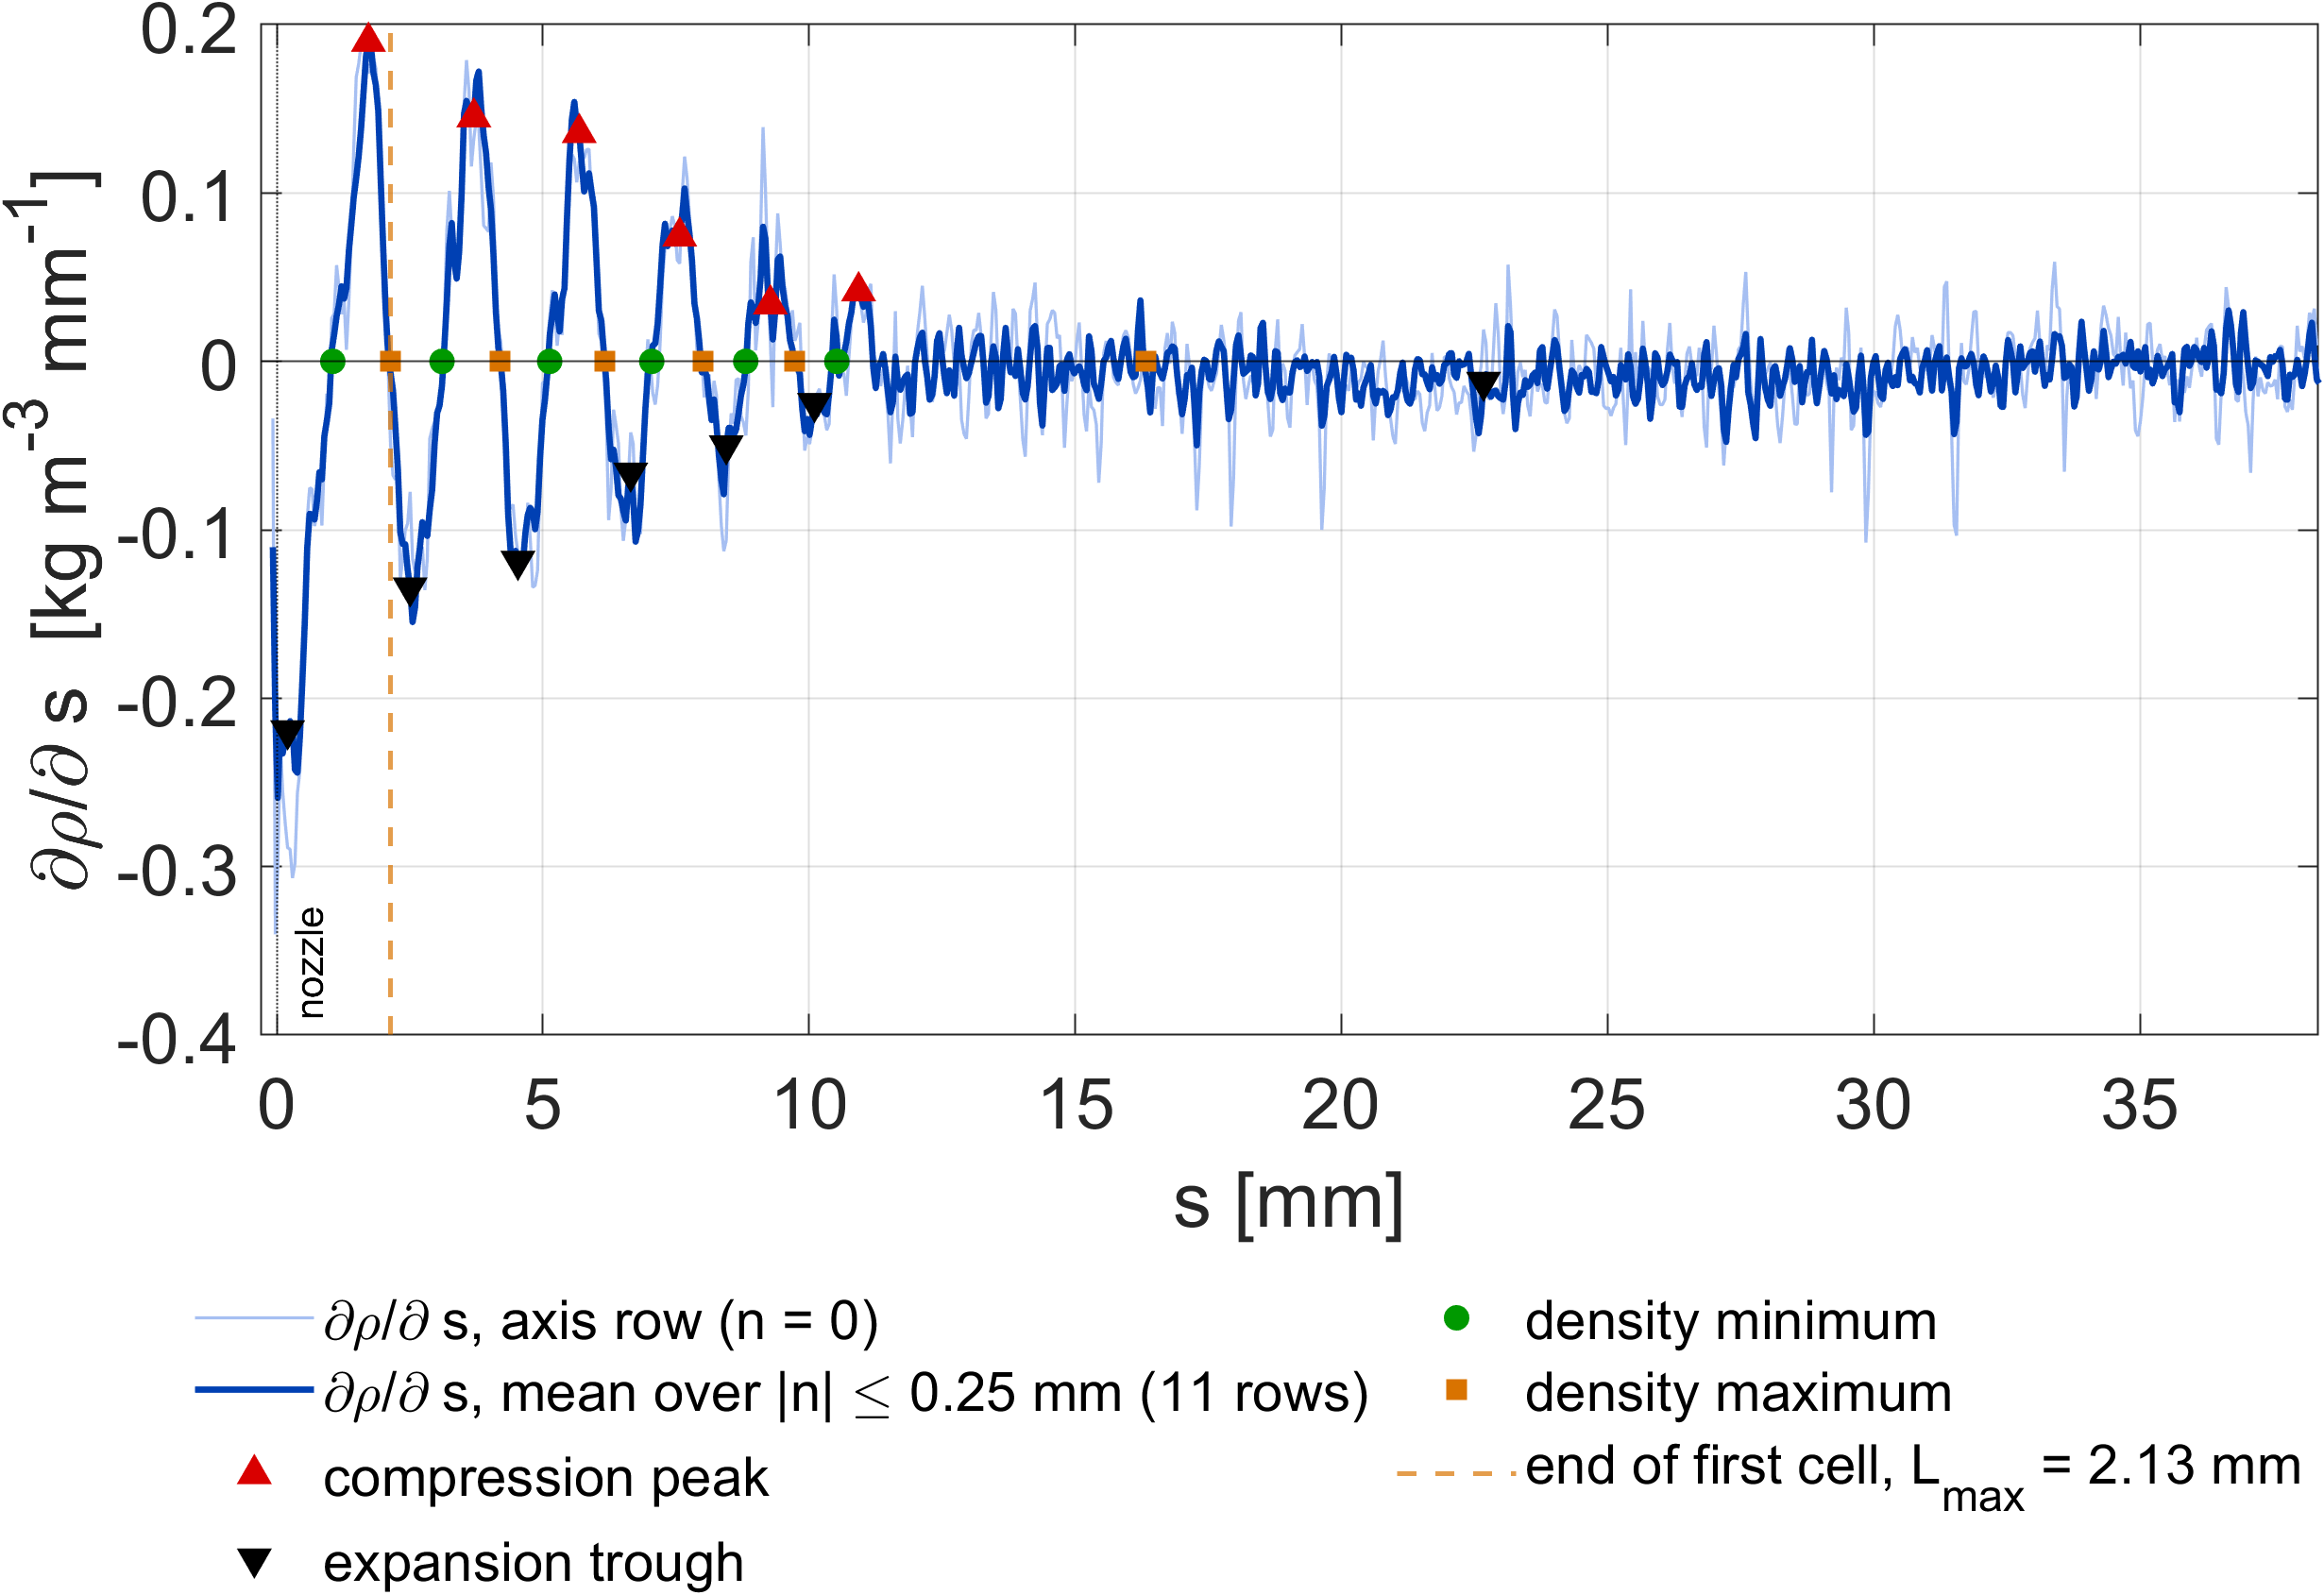
\includegraphics[width=\textwidth]{figures/centerline density gradient dataset a.png}
        \caption{Dataset a, with respective $NPR = 2.088$ and $L_s = 2.13$ mm}
        \label{fig: centerline density gradient dataset a}
    \end{subfigure}
    \hfill
    \begin{subfigure}[b]{0.32\textwidth}
        \centering
        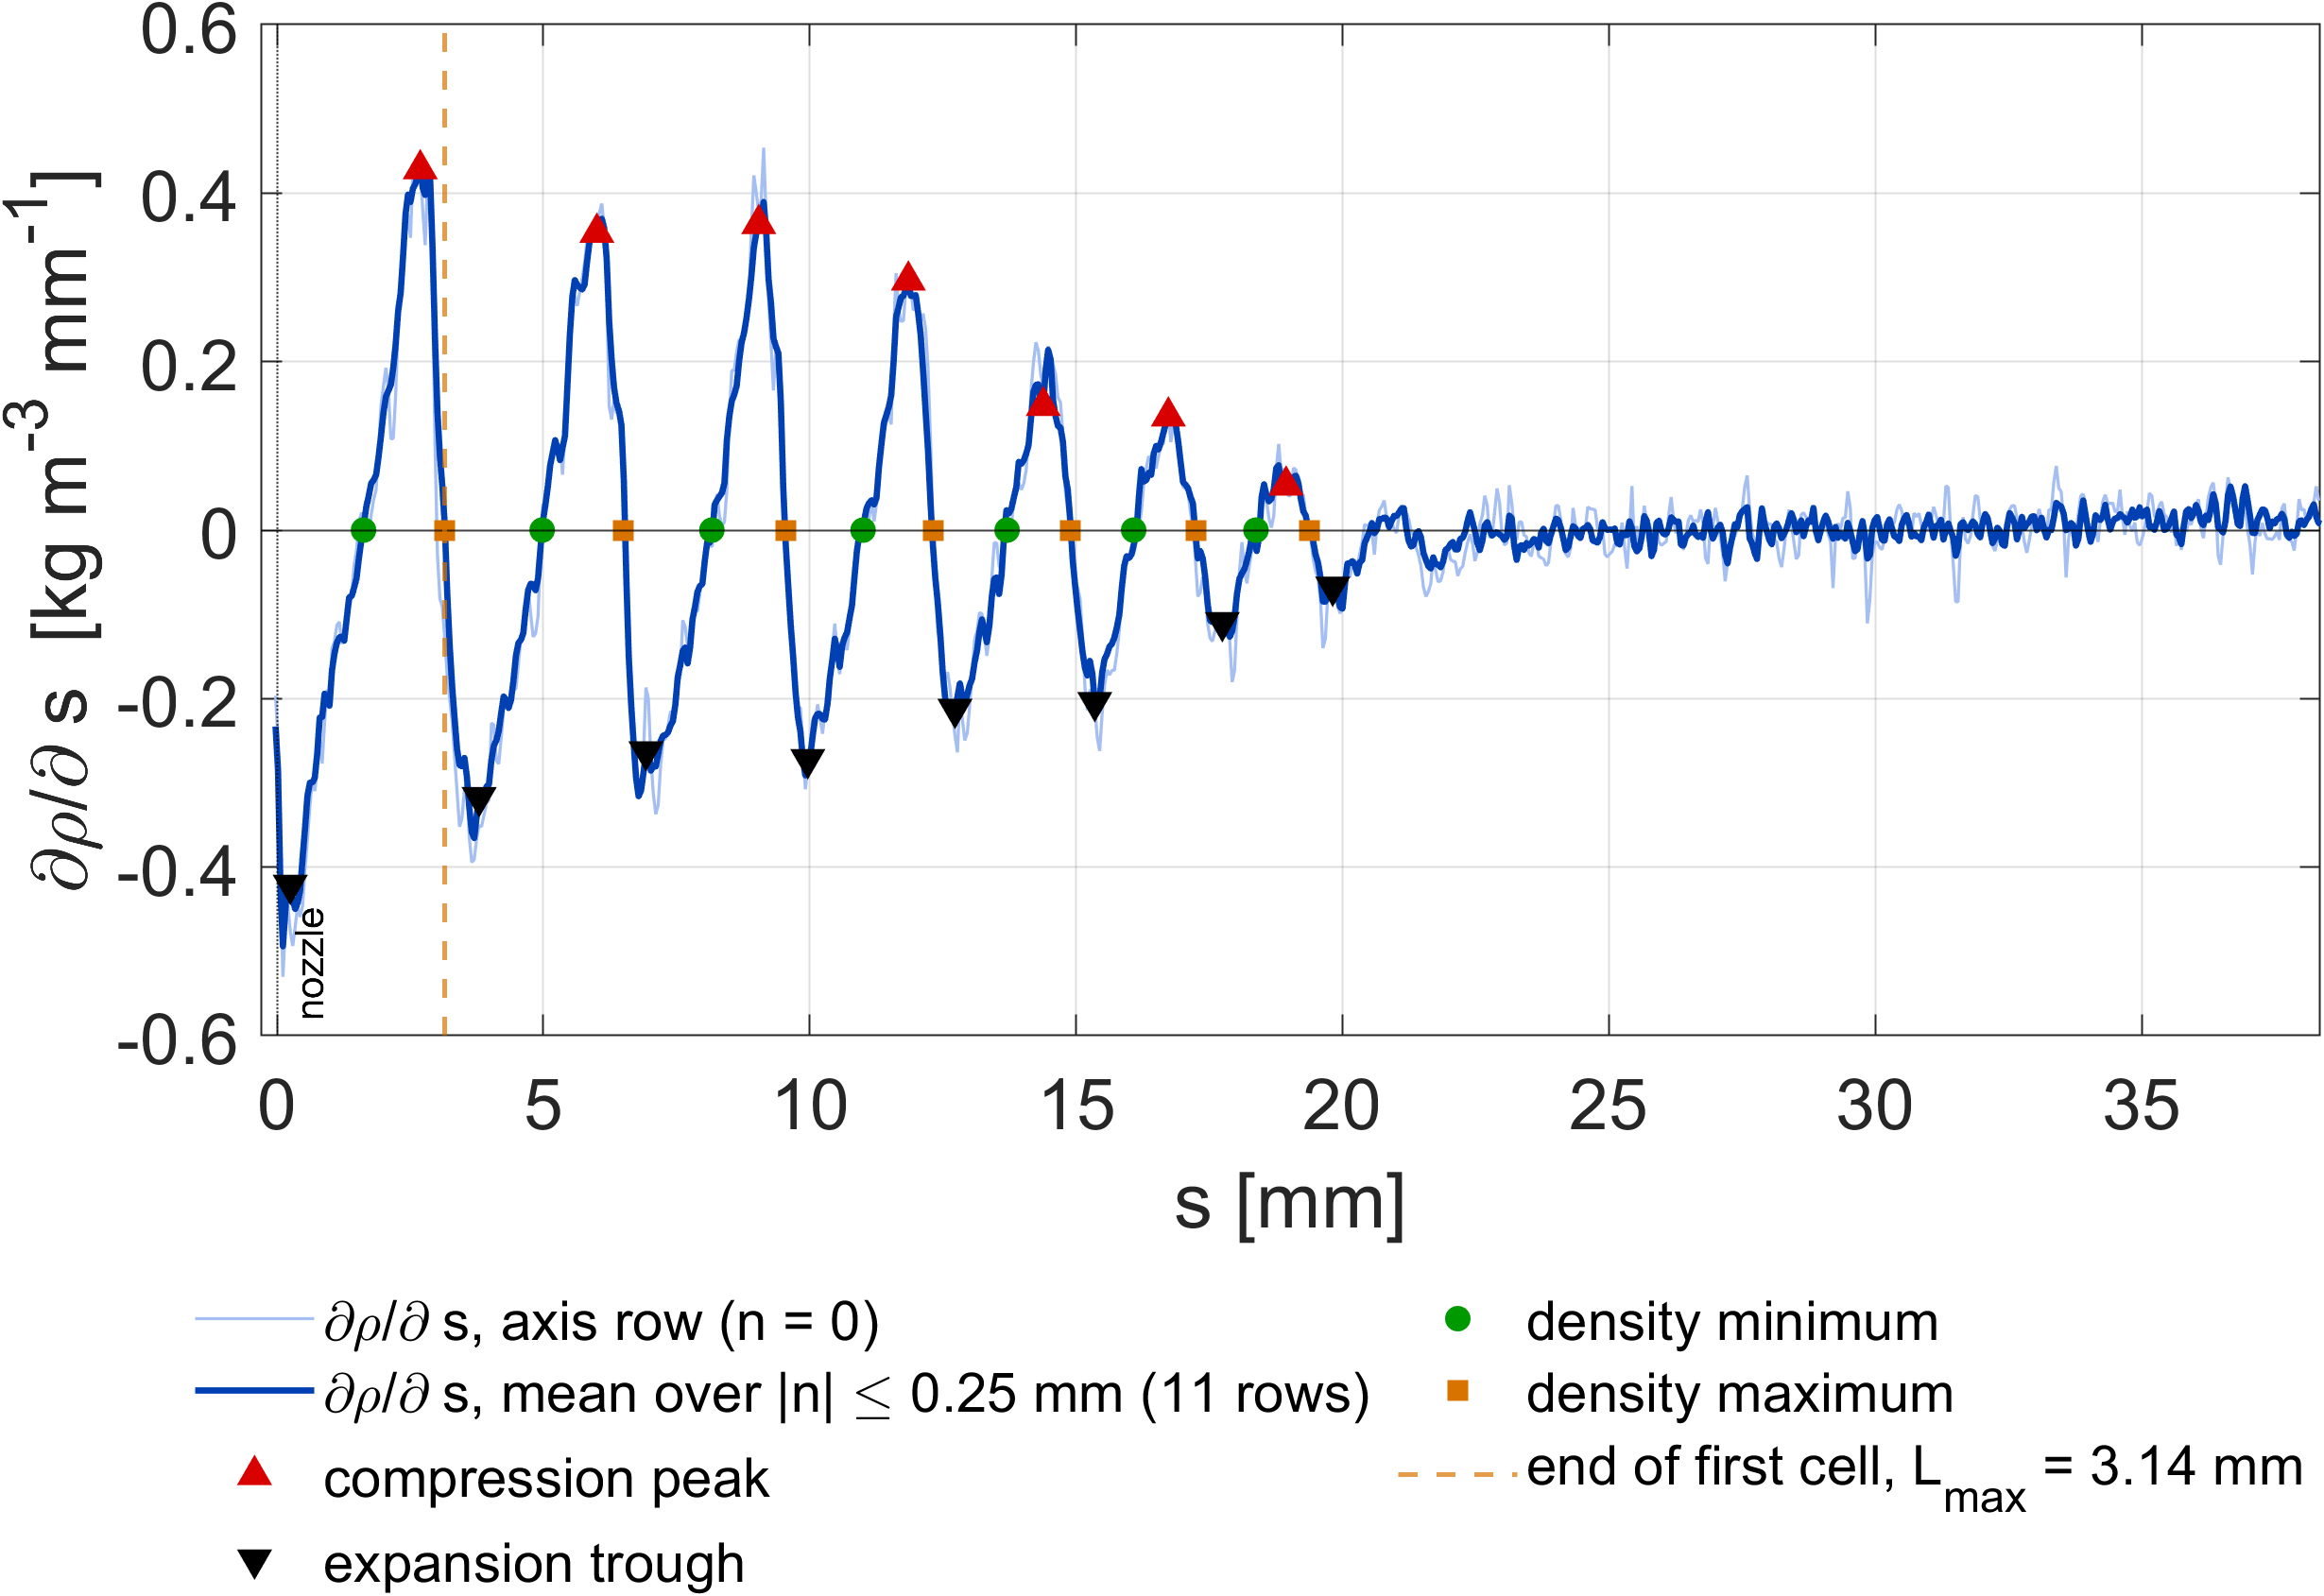
\includegraphics[width=\textwidth]{figures/centerline density gradient dataset b.png}
        \caption{Dataset b, with respective $NPR = 2.353$ and $L_s = 3.14$ mm}
        \label{fig: centerline density gradient dataset b}
    \end{subfigure}
    \hfill
    \begin{subfigure}[b]{0.32\textwidth}
        \centering
        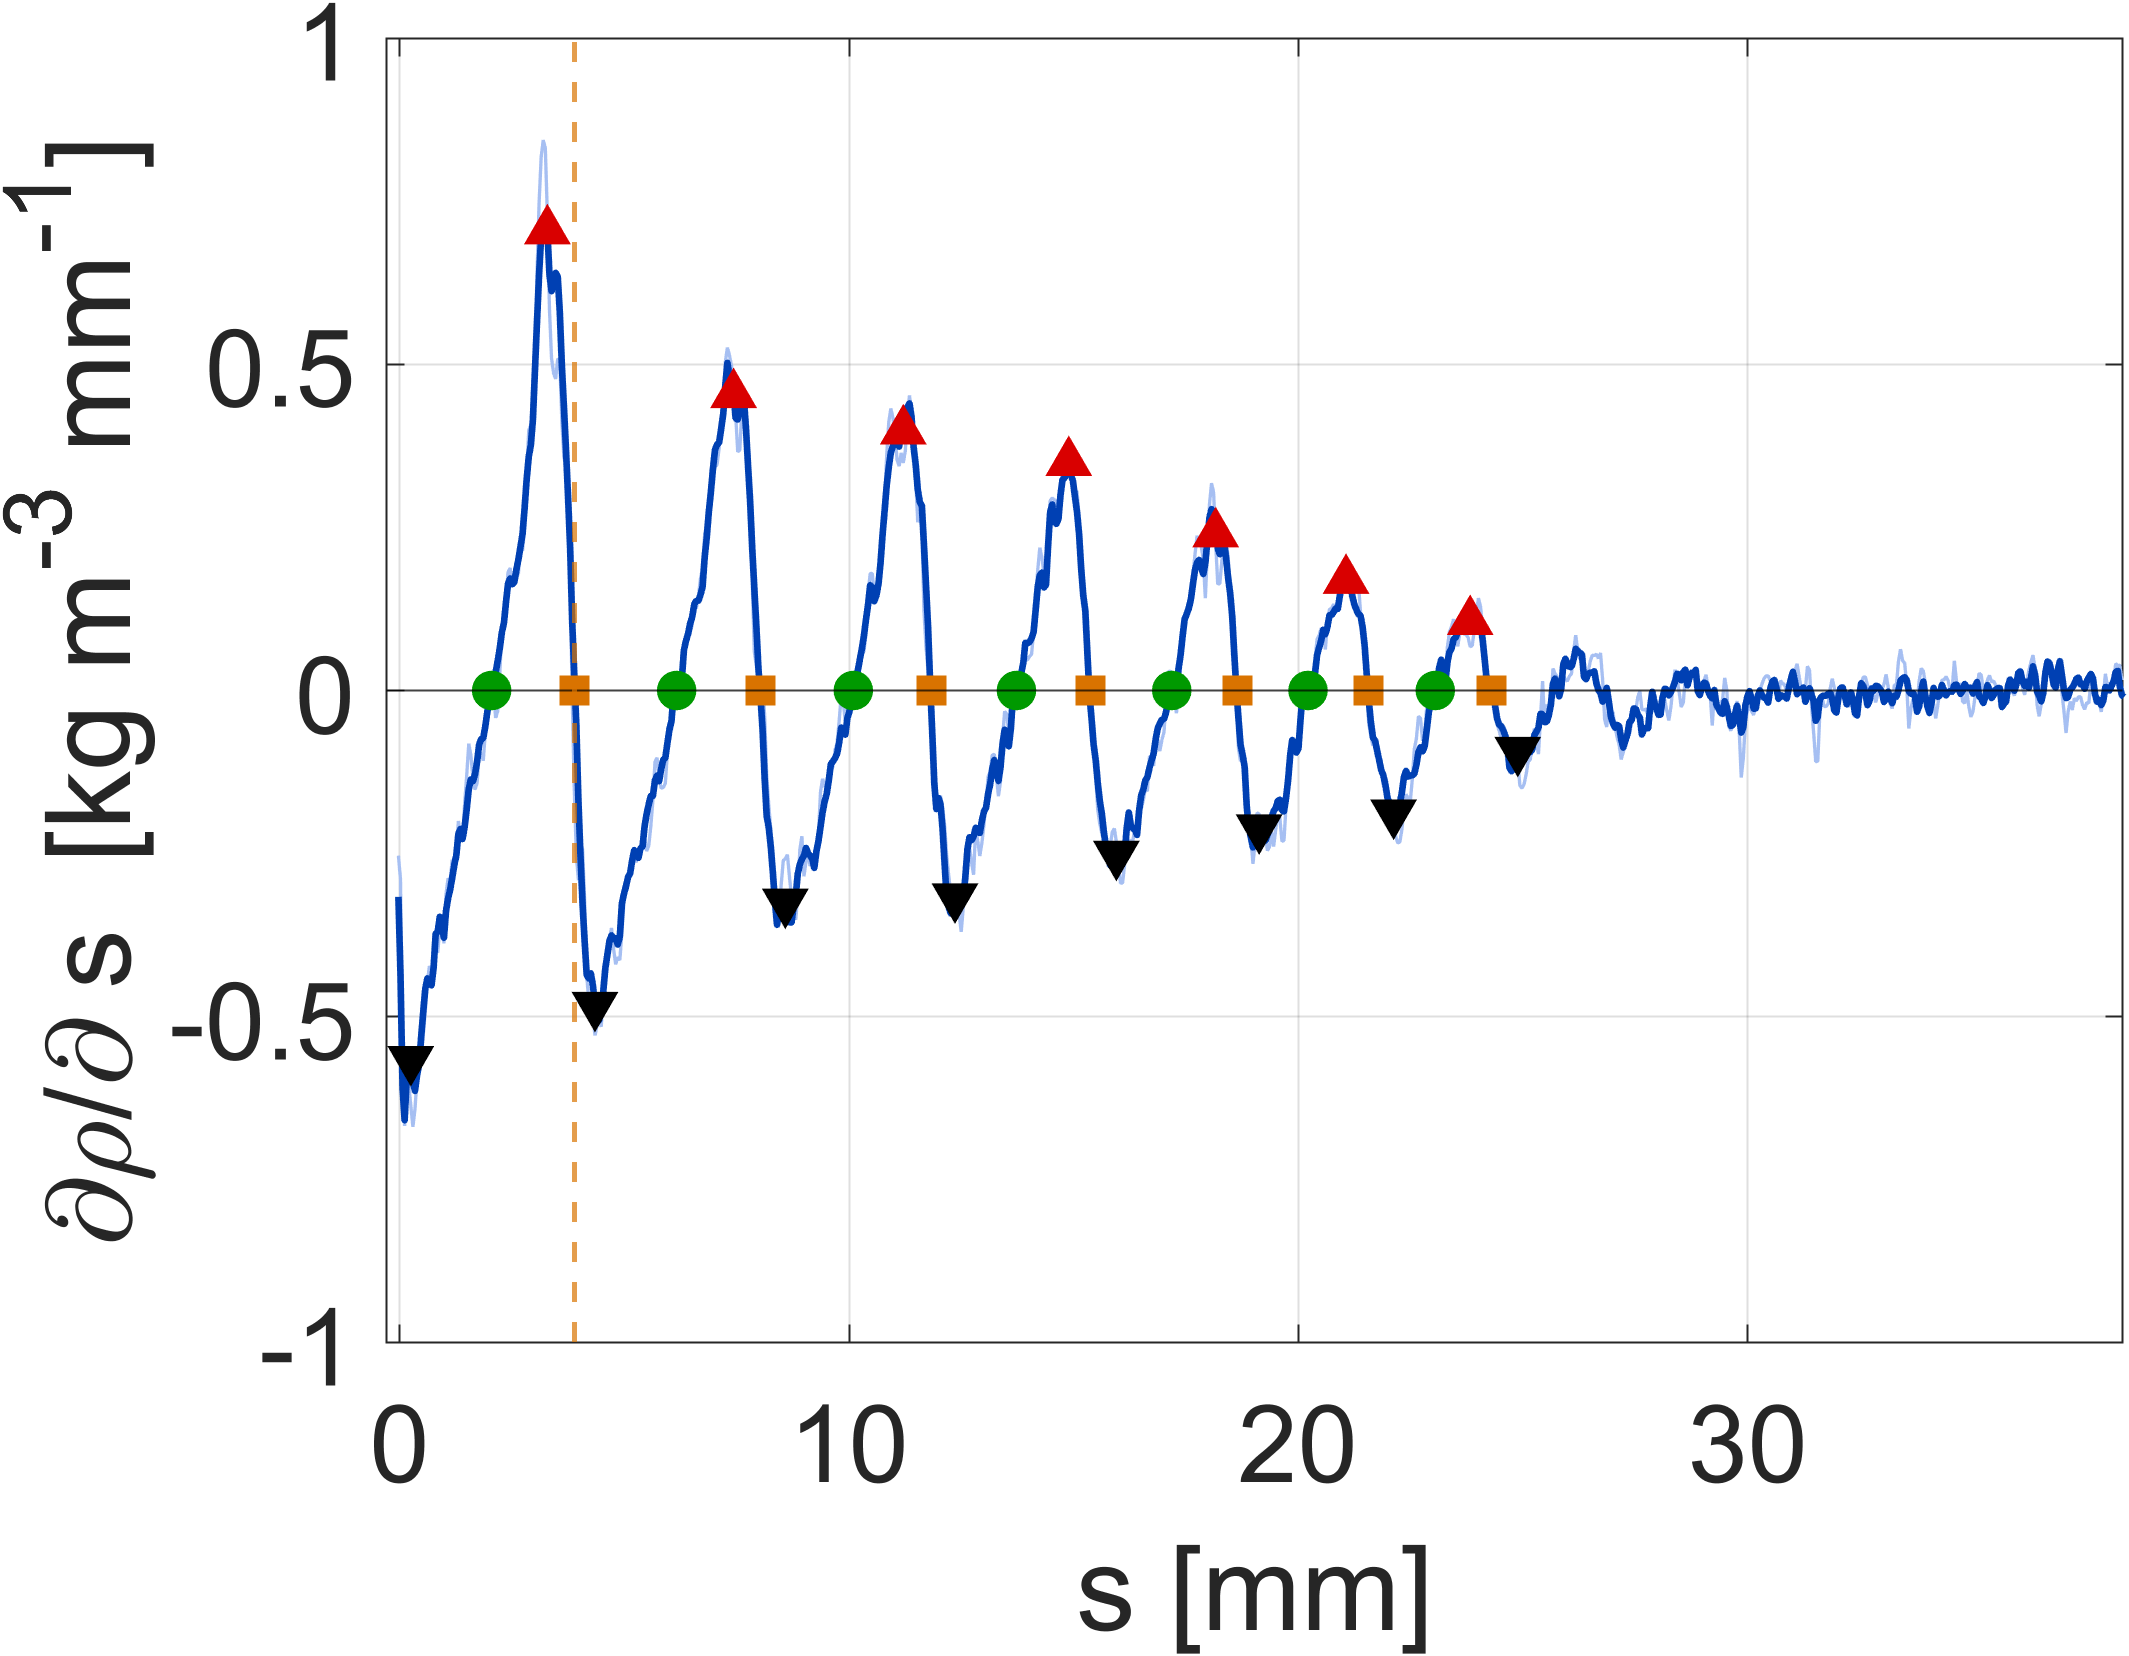
\includegraphics[width=\textwidth]{figures/centerline density gradient dataset c.png}
        \caption{Dataset c, with respective $NPR = 2.613$ and $L_s = 3.90$ mm}
        \label{fig: centerline density gradient dataset c}
    \end{subfigure}

    \vspace{0.5em}

    \begin{subfigure}[b]{0.32\textwidth}
        \centering
        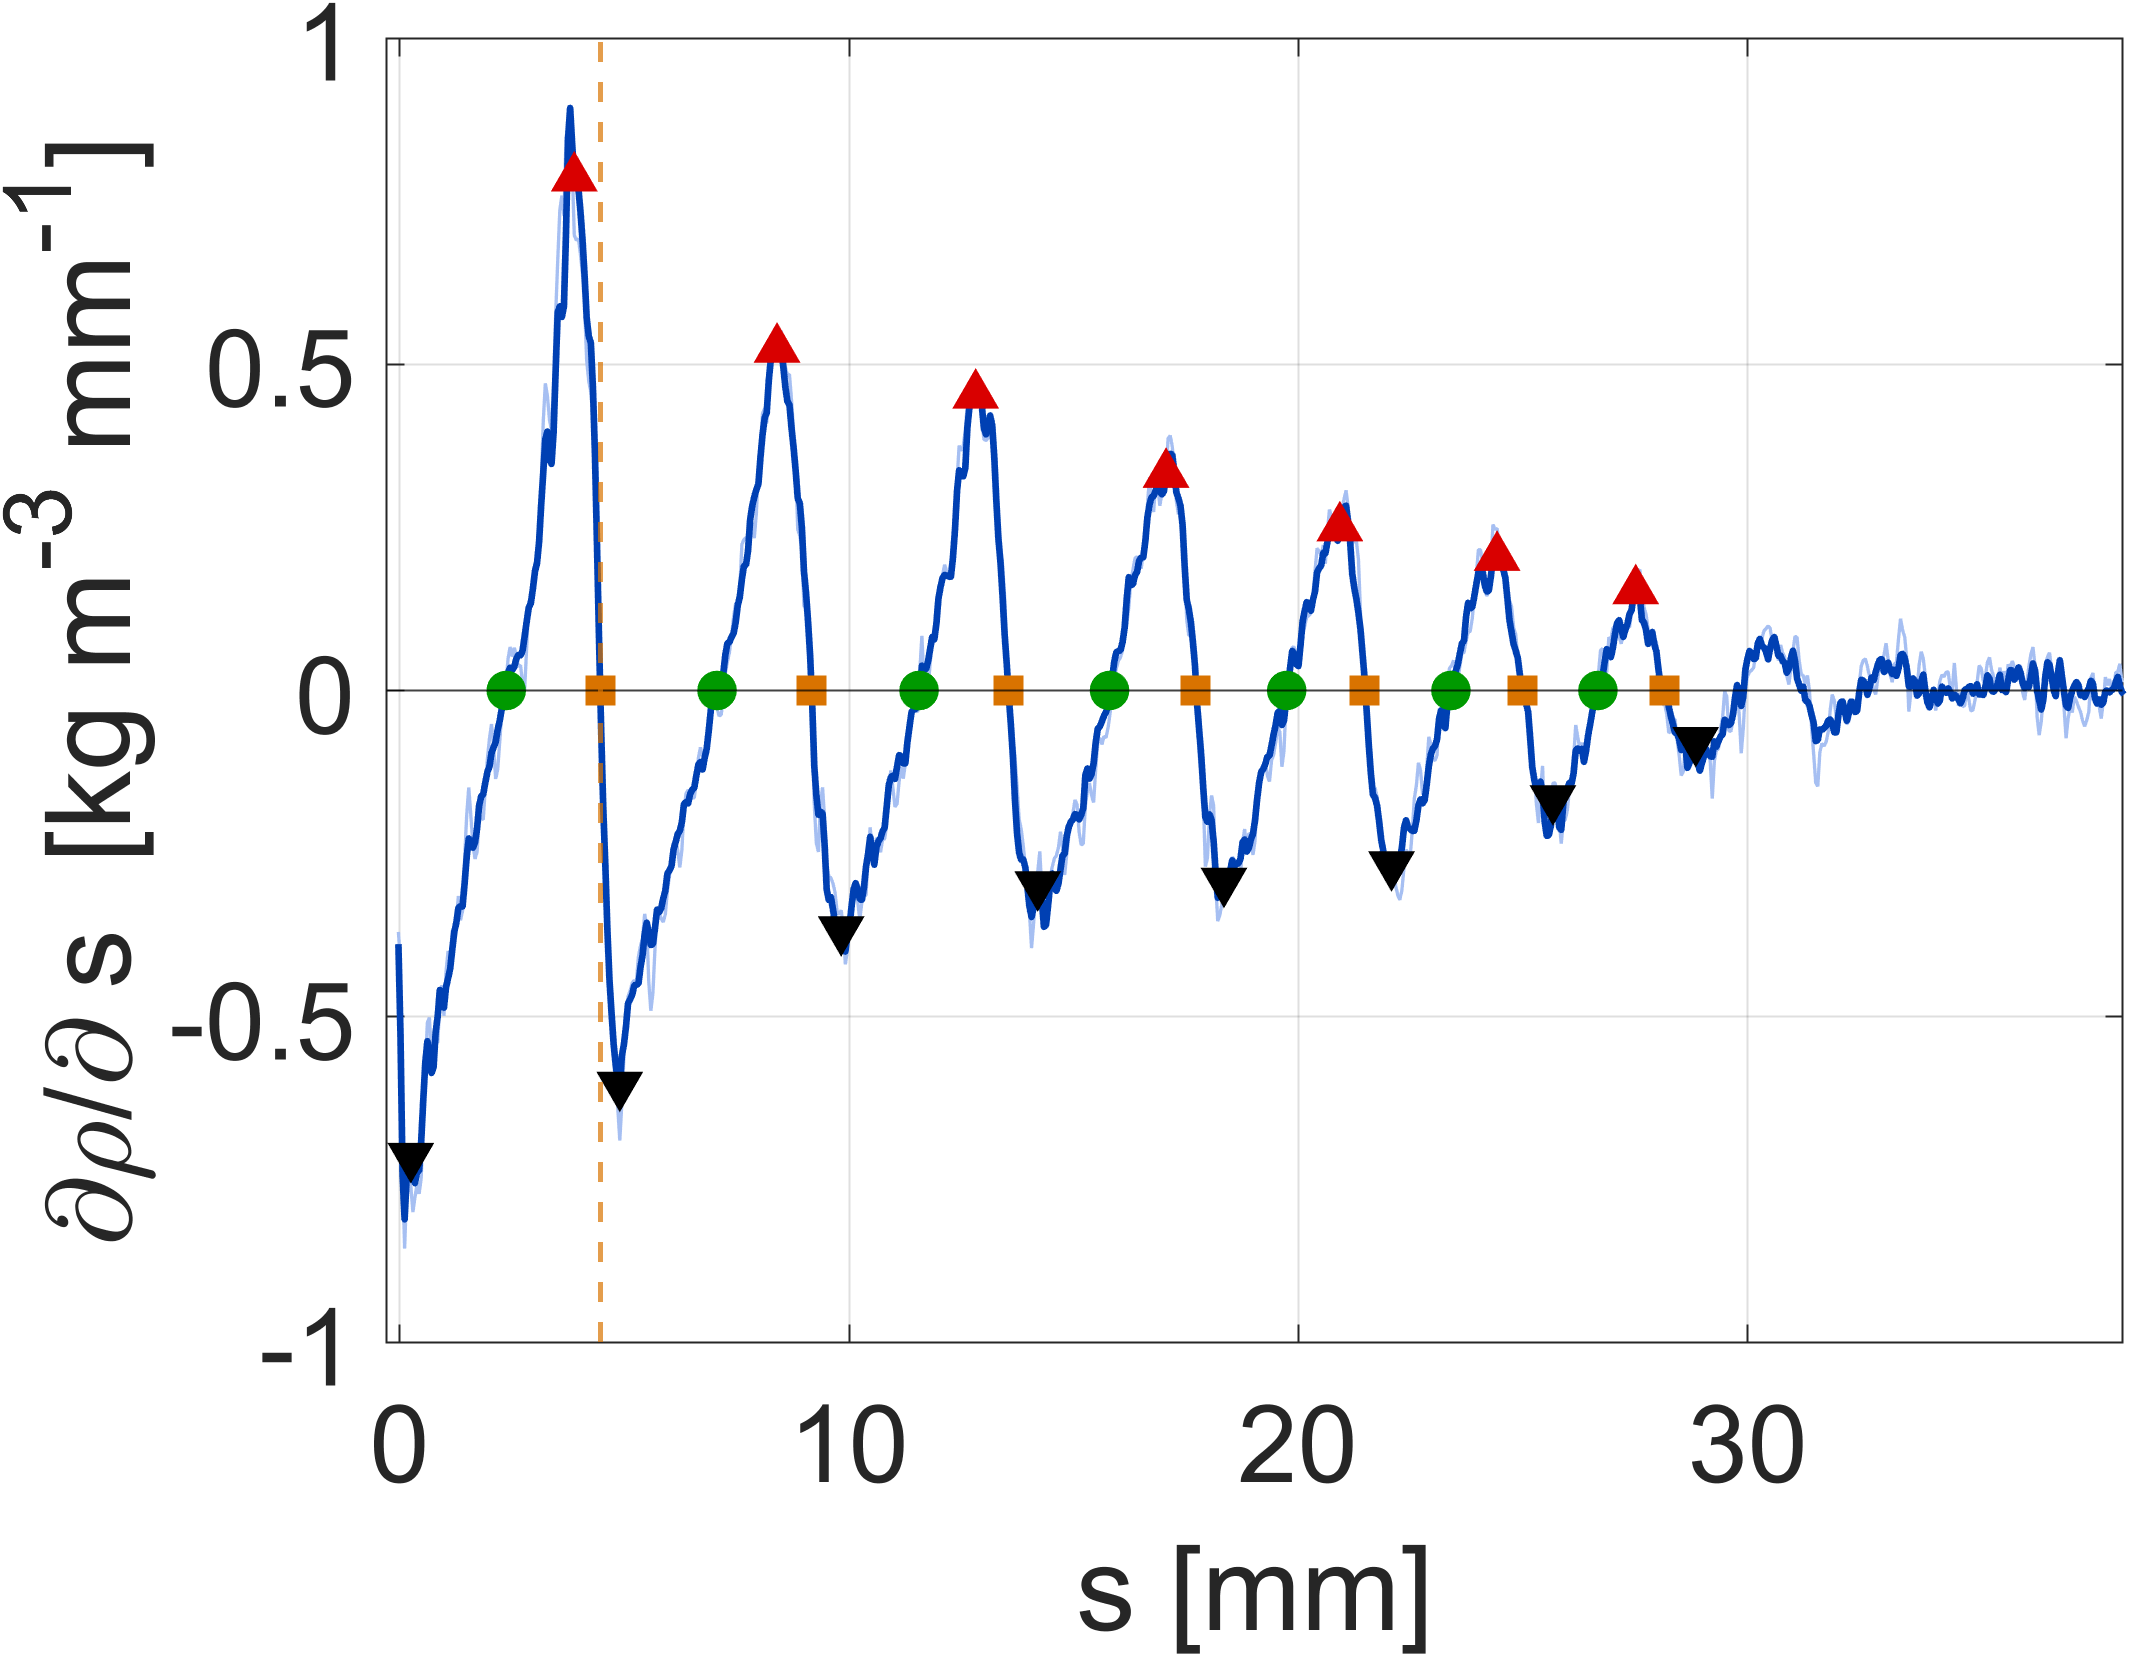
\includegraphics[width=\textwidth]{figures/centerline density gradient dataset d.png}
        \caption{Dataset d, with respective $NPR = 3.032$ and $L_s = 4.48$ mm}
        \label{fig: centerline density gradient dataset d}
    \end{subfigure}
    \hfill
    \begin{subfigure}[b]{0.32\textwidth}
        \centering
        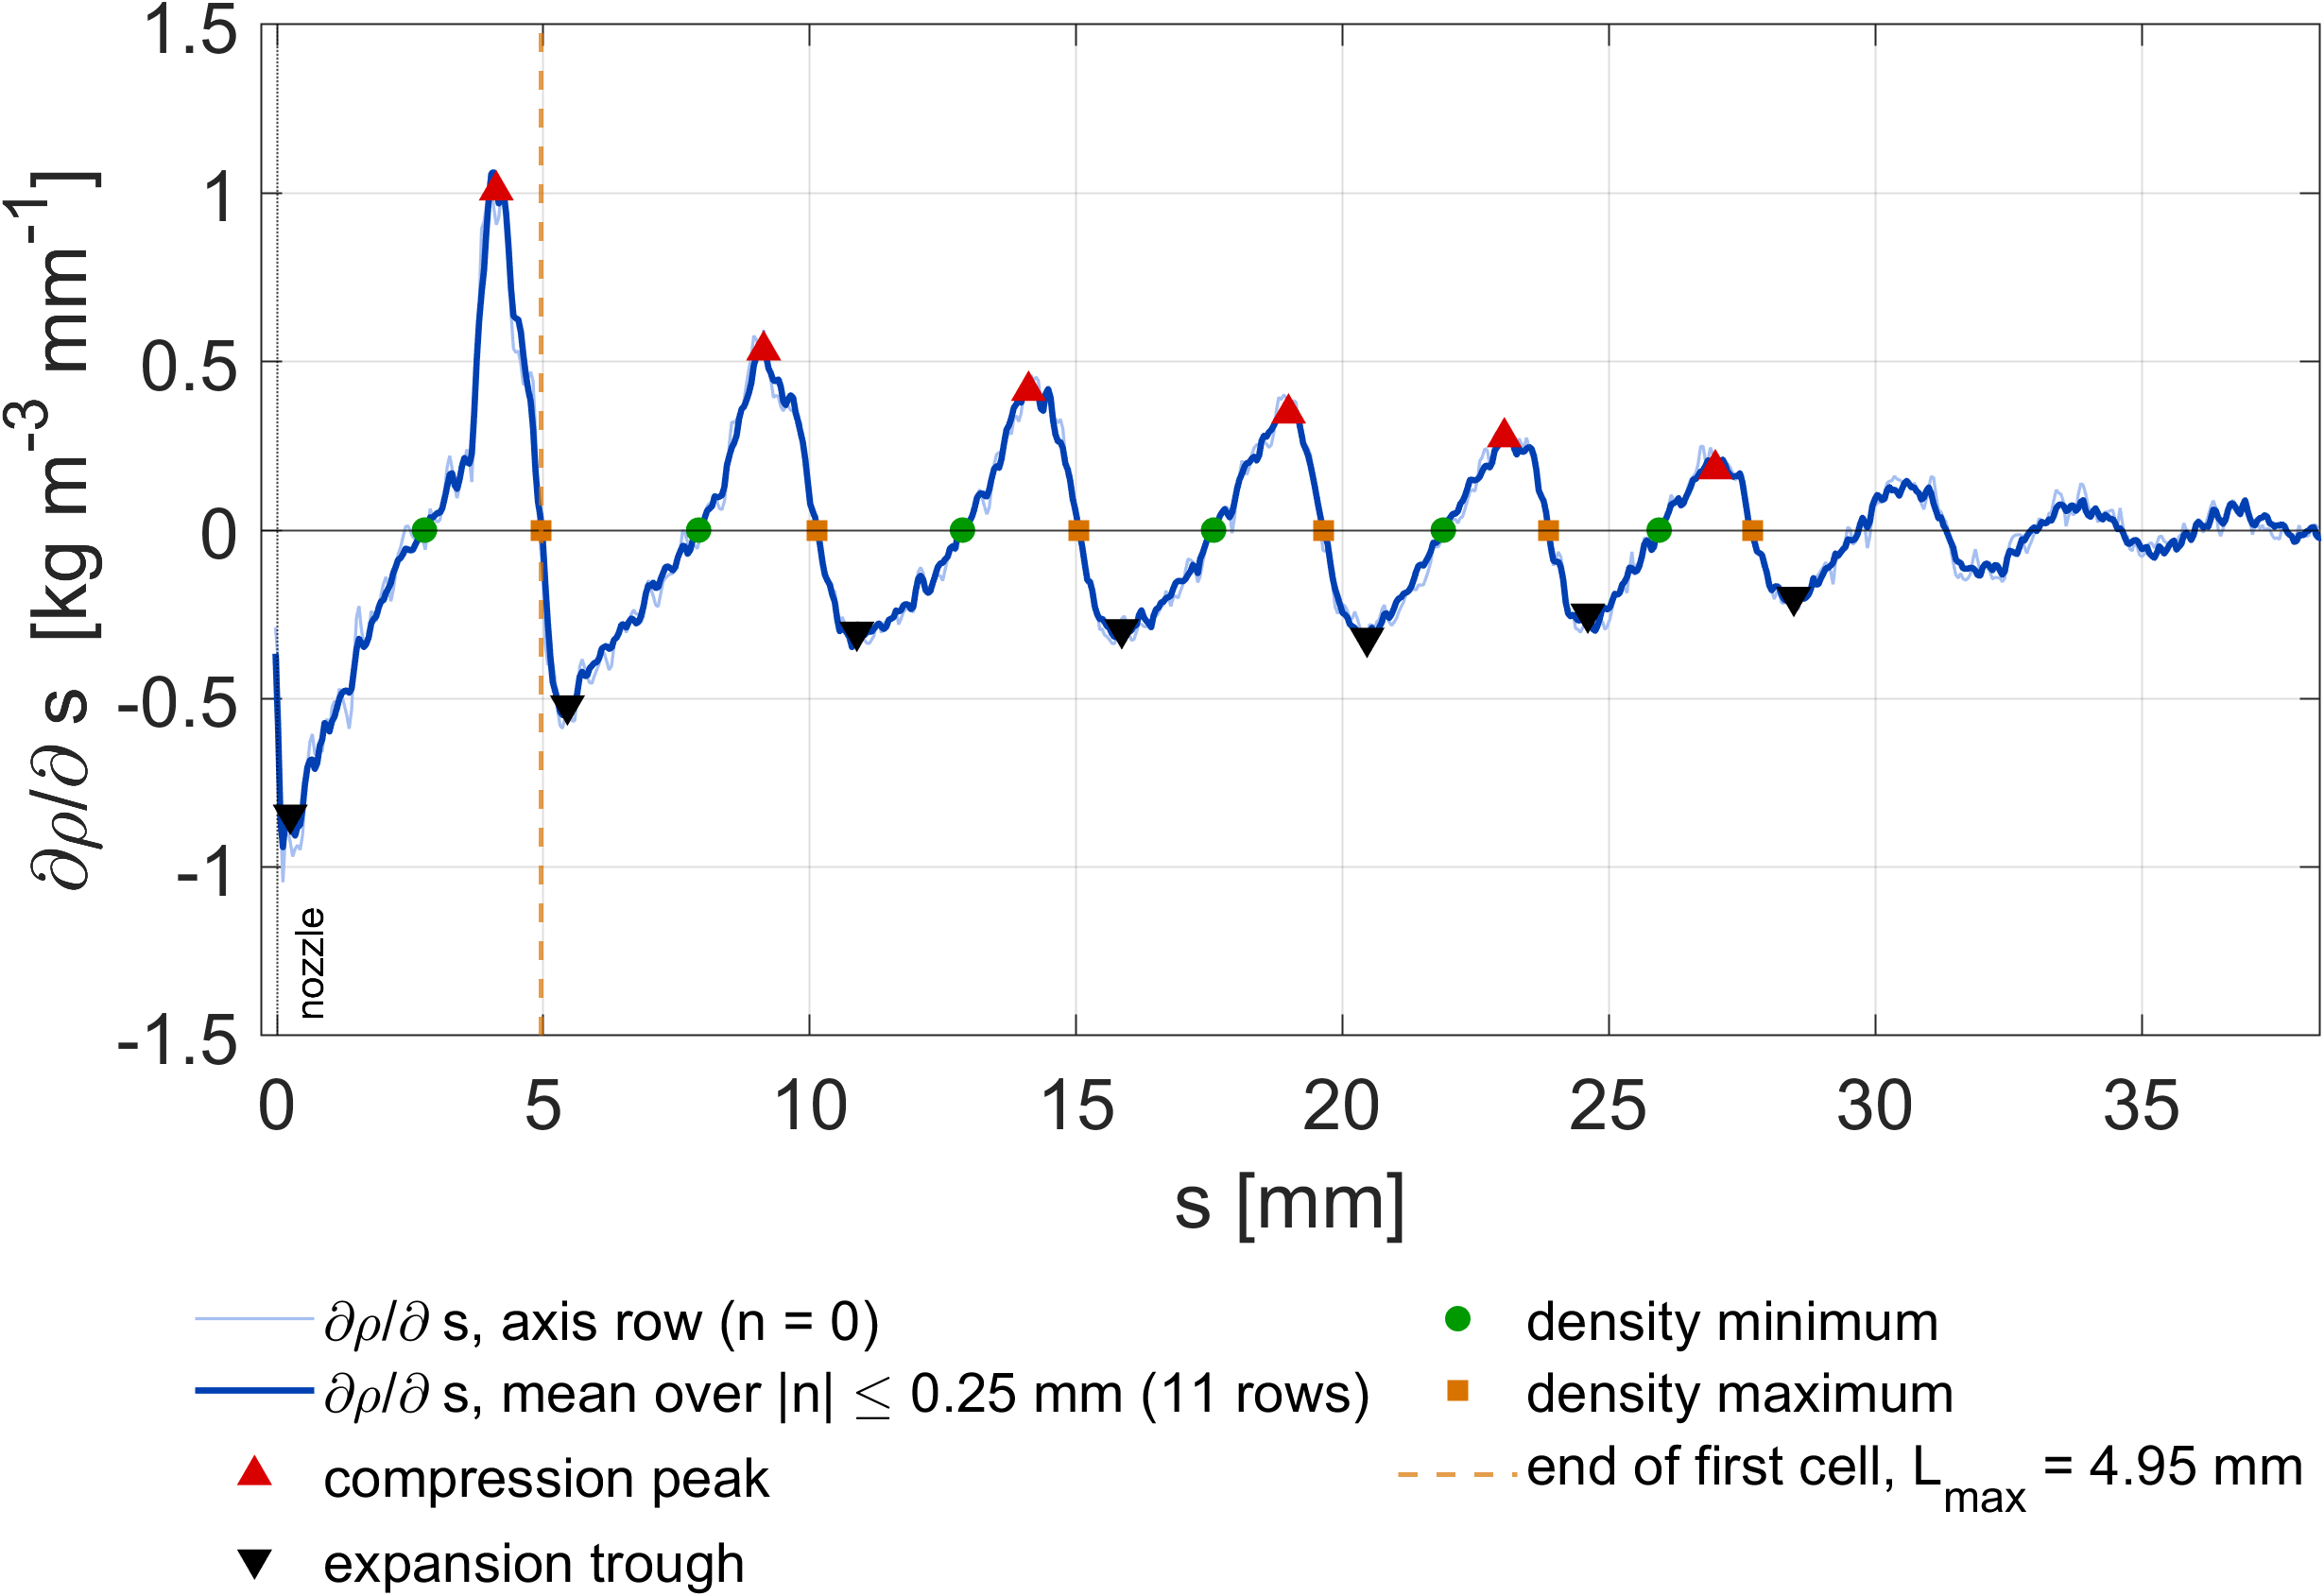
\includegraphics[width=\textwidth]{figures/centerline density gradient dataset e.png}
        \caption{Dataset e, with respective $NPR = 3.344$ and $L_s = 4.95$ mm}
        \label{fig: centerline density gradient dataset e}
    \end{subfigure}
    \hfill
    \begin{subfigure}[b]{0.32\textwidth}
        \centering
        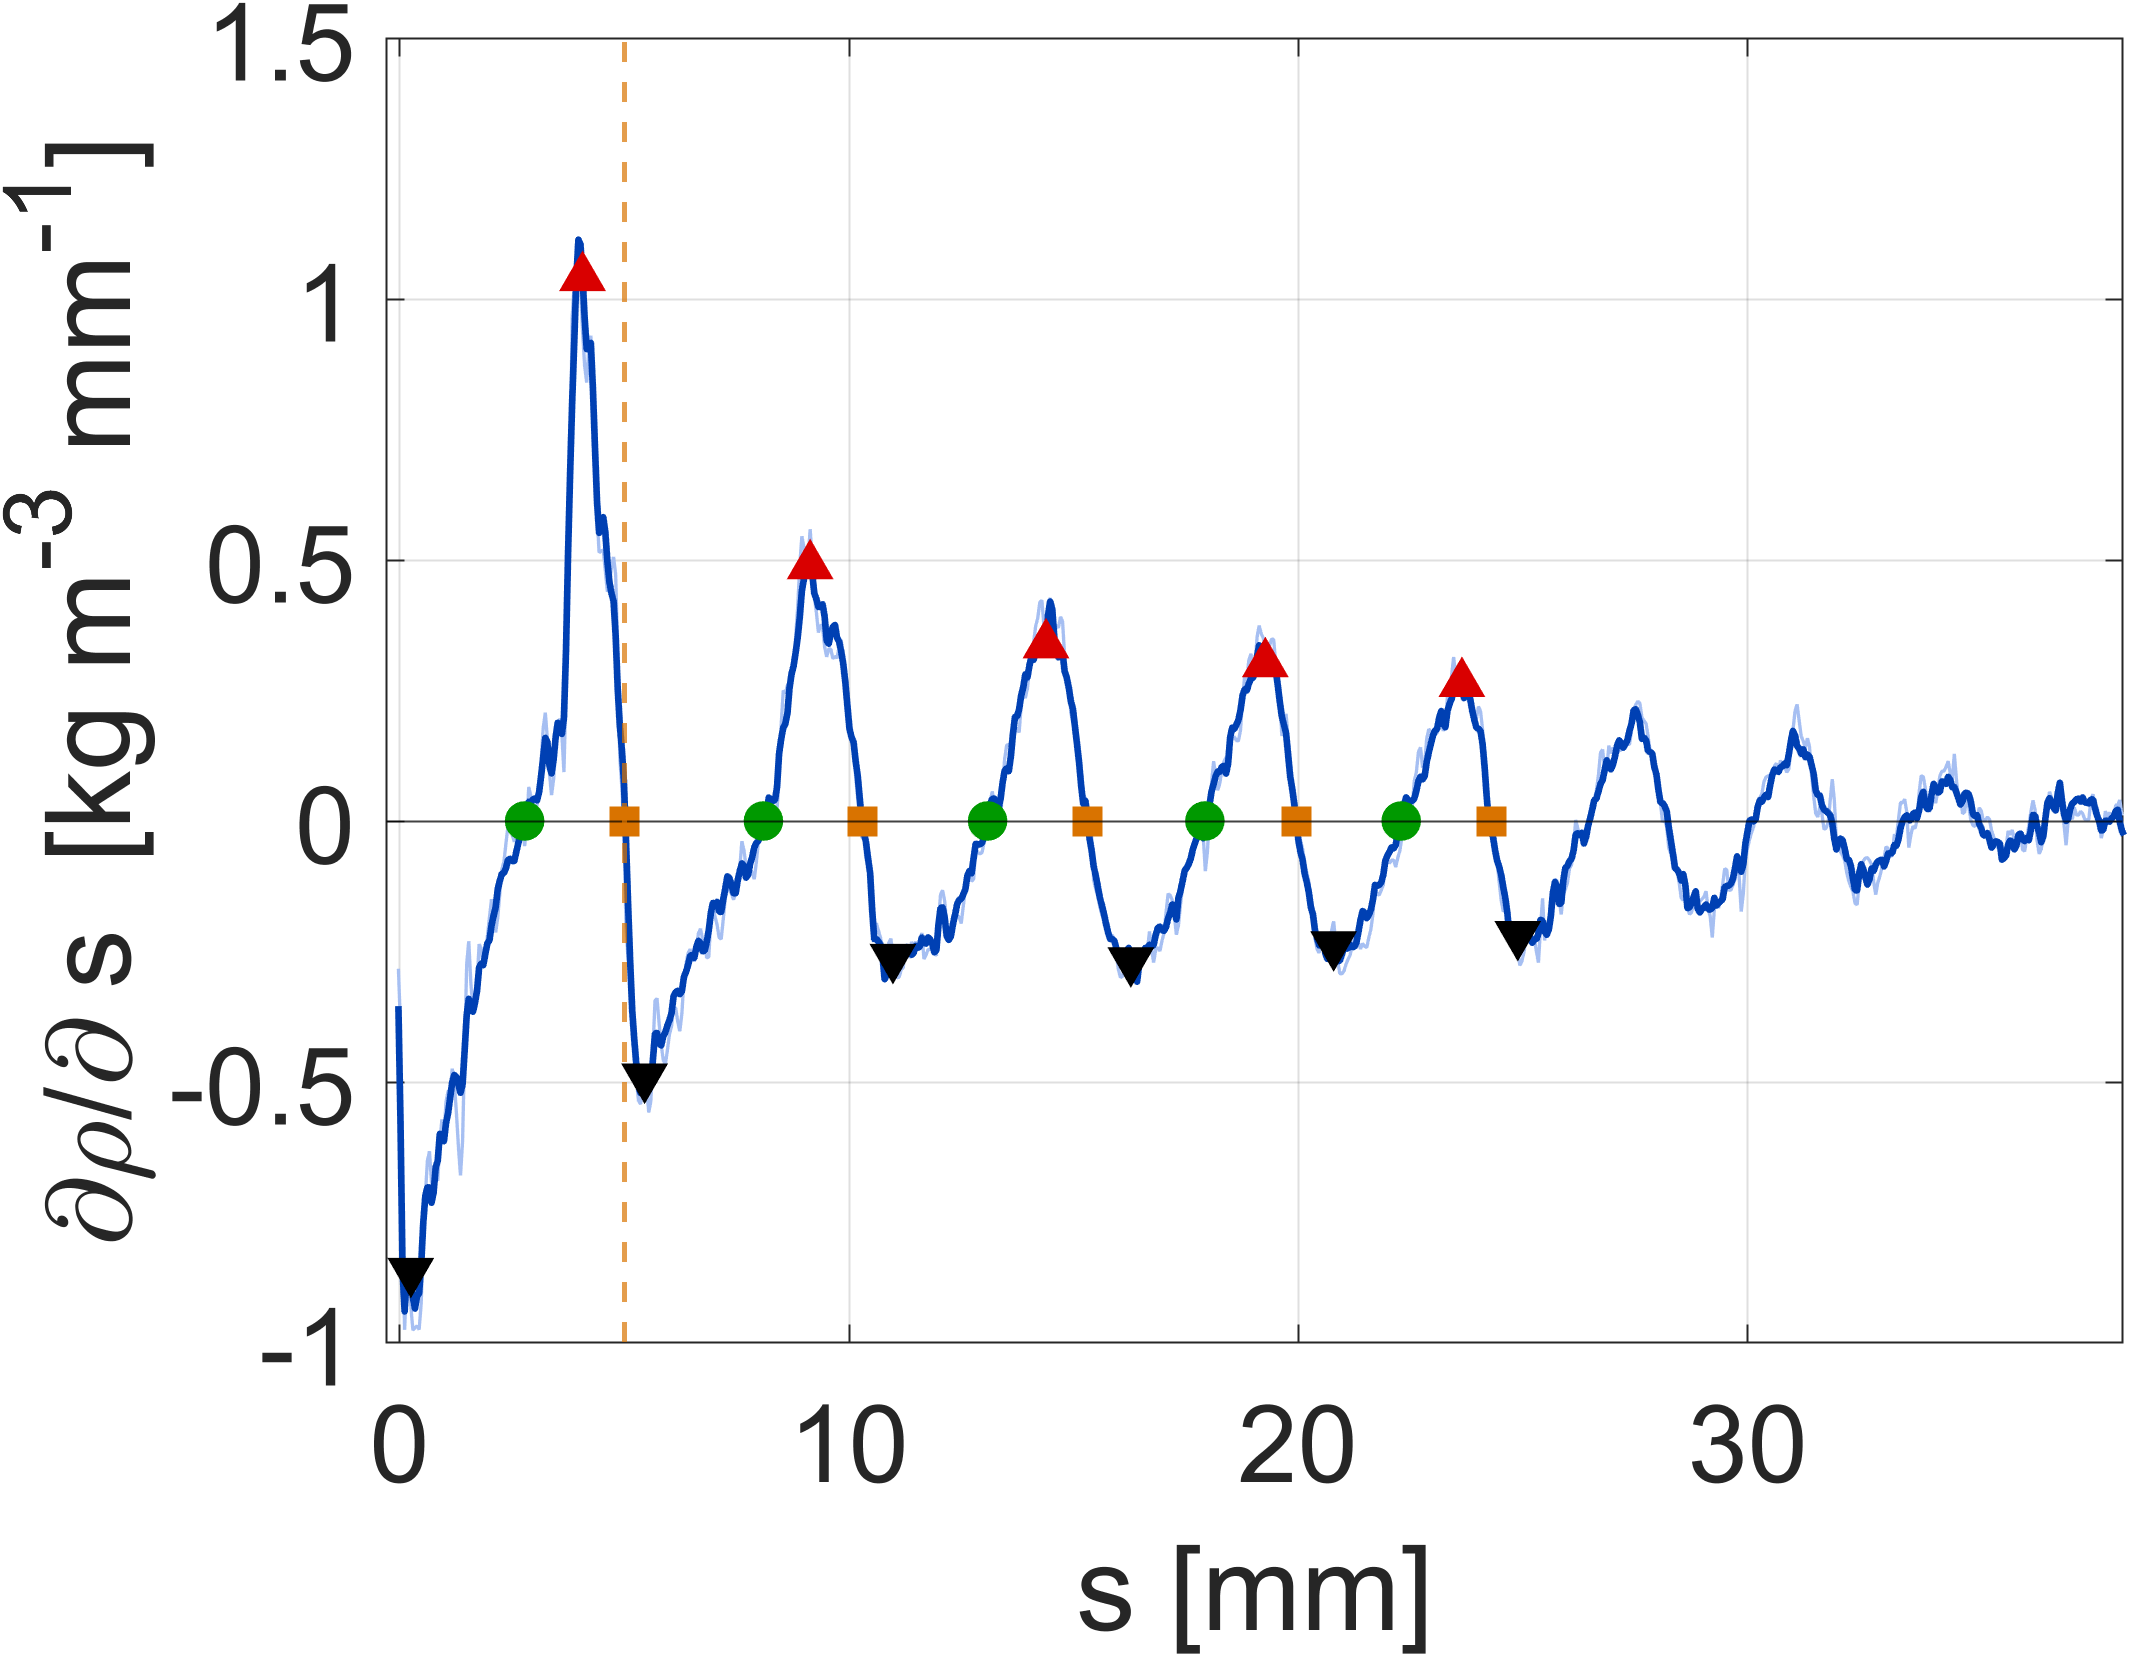
\includegraphics[width=\textwidth]{figures/centerline density gradient dataset f.png}
        \caption{Dataset f, with respective $NPR = 3.875$ and $L_s = 5.00$ mm}
        \label{fig: centerline density gradient dataset f}
    \end{subfigure}
    \caption{Centerline density gradient in the s direction for datasets a to f, obtained assuming a planar field. The light blue line is the gradient at the axis row $n = 0$ and the dark blue line its mean over $|n| \leq 0.25$ mm. Red upward triangles mark the compression peaks, black downward triangles the expansion valleys, green circles the density minima and orange squares the density maxima detected along the centerline. The dashed orange line marks the end of the first shock cell, $L_s$}
    \label{fig: centerline density gradients}
\end{figure}

% REVIEW: L_s is defined here as the distance between consecutive maxima, but the caption and the values use the nozzle to the first maximum. The NPR used for the fit comes from the shear layer angle, so the literature comparison checks consistency rather than validating the NPR independently.
The 6 plots in Figure \ref{fig: centerline density gradients} allow the identification of important marks in the shock cell structure. The periodicity and dissipation effect is clear, each cell is marked by an expansion valley and a compression peak and its amplitude decreases until atmospheric conditions are reached. The density maxima and minima are also distinguishable as the points where the gradient is zero. The distance between two consecutive maxima marks the length of the shock cell. For each dataset, the lengths of the first shock cell $L_s$ have been retrieved and they are displayed in their respective plot caption. The data confirms the previous qualitative visual evaluations regarding the shock cells sizes, as it shows that $L_s$ increases monotonically with $NPR$, meaning that the shock cells stretch further at increasing nozzle pressure ratios. It is also notable that more cells are present at higher pressures. Now that a more realistic estimate of the $NPR$ and $L_s$ have been achieved, it is possible to correlate both quantities using the formats of Equations \ref{equation: Emden Formula} and \ref{equation: Lazarus-Hartmann Formula} and compare to Emden's and Hartmann-Lazarus' formulation respectively, this way validating the application with literature data.

%Add shock cell length picture 

% REVIEW: Figure \ref{} is empty. The fitted L_s is the first cell, but Emden k = 0.88, Prandtl k = 1.2 and Hartmann-Lazarus k = 1.06 describe the later cells (average of later cells?); only the Hartmann-Lazarus constant-term formula (0.98, 0.30) is for the first cell. "Can be said to be satisfactory" is weak for a conclusion.
The fitted curves using Emden's and Hartmann-Lazarus' formulations are displayed together with the literature solutions in Figure \ref{}. The obtained values for the constants are: $k = 1.16, a = 0.894$ and $b = 0.28$. The $k$ value differs from Emden's $0.88$ figure, however, it is in line with other estimates such as Prandtl-Pack's $k = 1.2$ and Hartmann-Lazarus' $k= 1.06$ \cite{Emden1899, Hartmann1941, Powell2010}. Visually, the data is positioned in-between Hartmann-Lazarus' equation and Emden's formulation, as it slightly underestimates the former and considerably overestimates the latter. Regarding the fits, the Hartmann-Lazarus equation better describes the data behavior as the Emden format diverges significantly to the last point. Given that the data follows a trend format previously observed in the literature, is positioned in between two established results, and given the limitations of the measurements, the results can be said to be satisfactory.

\subsection{Quantitative Density Field results}
\label{subsection: Quantitative Density Field results}

One of the goals of the compressible jet experiment was the quantitative reproduction of its density field using the displacement data gathered with SBOS. In order to achieve that, the vector field had to go through a series of post-processing steps, integration schemes and noise regularization. The first ones were already mentioned, where the median of the background vector was removed and the image translated and rotated to position the jet axis horizontally at n = 0. Furthermore, the resulting displacements were averaged folded along n = 0. For the even function $\partial \rho / \partial s$  the symmetric components were summed and halved, while for the odd function $\partial \rho / \partial n$ the sum of the absolute symmetric components was halved. Placing the jet axis at n = 0 and folding it is of utmost importance for the implementation of the next step, as any anti-axissymetric feature will introduce errors. Next, an Abel inversion algorithm was implemented following the integration and inversion steps in the theory of section \ref{subsection: Axisymmetric Refractive Field}. An onion-peeling integration method described by Dasch \cite{} was implemented, together with a Tikhonov regularization scheme to smooth out noise, as studied by Daun \cite{}, with Generalized Cross Verification of Golub \cite{} to choose the Tikhonov parameter.

\section{Aerospike Experiment Results}
\chapter{Conclusion}
\label{chapter: Conclusion}

This thesis investigated the implementation of Laser-Speckled Background Oriented Schlieren in a supersonic wind tunnel. The method was approached through four experimental campaigns of increasing complexity that tackle each of its three main components: the optical configuration, the speckle generator and the refractive object. First, Chapter \ref{chapter: methodology} presented a design methodology developed to balance the sensitivity and spatial resolution of a SBOS setup to reach an optimal physical layout. This methodology was applied, tested and refined to design the experimental setups described in Chapter \ref{chapter: Experimental Setups}. Different optical configurations were tested to image the distortions produced by a simple refractive object, which allowed for the validation of the methodology and comparison of the various setups' performance parameters. A dedicated campaign investigated the production of speckle patterns, arriving at a configuration capable of producing speckles with average diameters between 2--5 px. Then, an under-expanded compressible jet served as a test subject for the quantitative density reconstruction of a real schlieren object using displacement fields obtained through SBOS. The final experimental campaign used the method to study the flow of a linear aerospike nozzle in a high-speed wind tunnel environment. The results gathered and discussed in Chapter \ref{chapter: Results} make it possible to answer the main research question and the five sub-questions posed at the start of this thesis in Chapter \ref{chapter: introduction}.

\section{Practical guidelines for the design of a SBOS setup}
\label{section: Research question 1}

The first research sub-question intended to discover what should be the practical guidelines for designing a SBOS setup. Chapter \ref{chapter: methodology} partially answered this question by summarizing the design guidelines resulting from the analysis of the design space surface maps. These recommendations survived the implementation in real experimental setups. However, further recommendations were collected throughout the duration of the thesis and can now be presented as a whole to aid the implementation of this technique by other researchers.

\textbf{Optical configuration.} The recommendations below follow from the design space analysis of Chapter \ref{chapter: methodology} and were confirmed, or qualified, by the angled glass campaign of Section \ref{section: Angled Glass Experiment Results}.

\begin{itemize}
    \item \textbf{A negative defocus configuration is preferable to a positive one.} For the same object field of view it reaches a higher optical magnification, which raises the sensitivity-resolution ratio of Equation \ref{equation: S over smin}. The slider experiment showed that the advantage comes from the shorter focal distance rather than from the sign of $l$, as the measured sensitivities are symmetric about the axis in Figure \ref{fig: S vs l slider experiment}.

    \item \textbf{A higher f-stop is desirable, within the limits imposed by the speckle size.} A larger $f_\#$ improves the trade-off without altering any physical distance, which makes it the most convenient parameter to adjust. It also reduces the illumination reaching the sensor and enlarges the speckle through Equation \ref{equation: Rayleigh Limit}, so it should be raised only while the pattern remains within the 2--5 pixel range.

    \item \textbf{A longer focal length tends to make the setup more robust.} A longer $f$ widens the spacing between isolines in the design space, so the performance parameters become less sensitive to positioning errors during assembly. It also raises the sensitivity ceiling of a positive defocus setup, given by Equation \ref{equation: BOS Sensitivity limit}. A moderately shorter lens can be adopted when the physical size of the setup is constrained, at little cost in sensitivity and spatial resolution.

    \item \textbf{The SR criterion can be used to match the optical and processing resolutions.} Equation \ref{equation: SR} expresses the minimum distinguishable feature in pixels, which allows the interrogation window to be selected so that neither the optics nor the cross-correlation limits the measurement unnecessarily.

    \item \textbf{Very short defocus distances are better avoided.} Although a short $|l|$ is favorable in a negatively defocused setup, the uncertainty budget of Table \ref{tab: measurement uncertainty} shows the contribution of $l$ becoming dominant below roughly 10 mm, where the combined uncertainty reaches 6.75\%.

    \item \textbf{The magnification is better measured on site than taken from the design.} The distances prescribed by the design methodology could not be reproduced exactly with a compound camera lens, since the equivalent thin lens position shifts with the imaging distance. The optical magnification should therefore be taken from a calibration target at the in-focus plane rather than from the design values.
\end{itemize}

\textbf{Speckle generator.} The recommendations below were obtained from the speckle pattern investigation of Section \ref{section: Speckle Pattern Experiment Results}, and several of them correct assumptions made before that campaign.

\begin{itemize}
    \item \textbf{A low power laser is sufficient.} The class 2 continuous laser of 0.5 mW used in this work produced a pattern of adequate contrast, because the speckle field is imaged directly rather than reflected from a printed background. The high luminous contrast also permits the short exposure times required to freeze fast phenomena.

    \item \textbf{The diffuser and the beam should be sized to the field of view.} The diffuser should be large enough to cover the desired object field of view, and the beam should be expanded to illuminate it. A beam that is too narrow becomes diffraction limited at the diffuser rather than at the lens pupil, which enlarges the speckle and removes its dependence on the aperture. This was the cause of the oversized speckles of the first campaign, where a diffuser of 1.27 cm was used with an unexpanded beam, and it is quantified in Figure \ref{fig: speckle dGG sweep}.

    \item \textbf{The speckle size is best tuned with the f-stop.} The measured speckle size followed the aperture as expected, whereas sweeping the optical magnification produced almost no change, as displayed in Section \ref{subsection: Speckle Aperture and Magnification}. With a compound camera lens the aperture appears to be the only reliable handle on the speckle size.

    \item \textbf{The Rayleigh limit is better treated as a preliminary estimate.} Once the beam was properly expanded the measured sizes fell within the same order of magnitude as Equation \ref{equation: Rayleigh Limit}, but deviations of up to 2.88 px remained. The relation is useful for sizing a setup and should not be relied upon for a final figure.

    \item \textbf{Either generation method may be used.} Projected and directed speckles produced patterns of comparable size and deviation, so the choice depends on practical considerations. Projected speckles suit applications with a single optical access or a laser powerful enough to damage the sensor, while directed speckles provide more intensity and therefore shorter exposures.

    \item \textbf{The diffuser should be isolated from vibration.} Any movement of the diffuser displaces the whole pattern, which introduces a spurious uniform shift and may lead to decorrelation.
\end{itemize}

\textbf{Refractive object.} The final set of recommendations concerns the object under study, and follows from the compressible jet and aerospike campaigns of Sections \ref{section: Compressible Jet Experiment Results} and \ref{section: Aerospike Experiment Results}.

\begin{itemize}
    \item \textbf{The defocus should be matched to the strength of the density gradients.} In a flow with strong gradients and considerable turbulence, the defocused configurations blurred the speckle pattern to the point of decorrelation, and the resulting displacement fields were dominated by noise, as shown in Figure \ref{fig: aerospike displacement points 1-3}. The blur originates partly from the flow itself and cannot be removed by reducing the aperture alone.

    \item \textbf{Focusing inside the test section might be preferable when the gradients are strong.} Placing the in-focus plane within the flow removed the decorrelation and produced the most detailed results of the aerospike campaign, capable of rivaling the schlieren images of the same condition.

    \item \textbf{The sensitivity can be recovered from the ratio of measured displacements.} When the in-focus plane lies inside the test section the sensitivity cannot be estimated as $S = l \cdot M_{ag}$. If the same flow is imaged at a second configuration of known sensitivity, Equation \ref{equation: S ratio} provides an estimate, which agreed with the geometric value within 5\% in Table \ref{tab: S ratio}.

    \item \textbf{The thickness of the test section should be accounted for.} Where the flow is separated from the camera by windows, the lever arm becomes $l_{eff} = l + G + W/2$, which degrades the spatial resolution. In the wind tunnel campaign this doubled the minimum distinguishable feature from 10 to 20 pixels, and it should be included in the design rather than added afterwards.

    \item \textbf{The density gradients can be verified through an independent configuration.} Imaging the same flow condition twice, with different optical arrangements, allows the scaling from displacement to density gradient to be checked by comparing the peak values, as presented in Table \ref{tab: aerospike gradient peaks}.

    \item \textbf{The nominal flow conditions might not be reliable.} The nozzle pressure ratios estimated from the wall gauge disagreed with the observed shock cell structure, and the losses through the line exceeded 40\%. A ratio estimated from the flow itself, in this case from the shear layer angle at the nozzle lip, proved considerably more reliable, as displayed in Table \ref{tab: compressible jet NPR estimates}.
\end{itemize}





%% Prevent urls running into margins in bibliography
\setcounter{biburlnumpenalty}{7000}
\setcounter{biburllcpenalty}{7000}
\setcounter{biburlucpenalty}{7000}

%% Add bibliography
\printbibliography[heading=bibintoc,title=References]

%% ----------------------------------------------------------------------
%%    Appendix (Letters for chapters)
%% ----------------------------------------------------------------------

\appendix

\chapter{Derivation of the Circle of Confusion}
\label{Appendix: CoC derivation}

The Circle of Confusion estimates through classical optical theory the amount of blur present in the image of an out of focus object, as explained by Greenleaf \cite{Greenleaf1950}. As shown in Figure \ref{fig: CoC geometry}, an object $O$ at a distance $d_f$ of a converging lens, with focal length $f$ and aperture $D$, produces an image $I$ at a distance $Z$ of this lens, as per the ideal lens equation. If an object $O'$ finds itself behind of $O$ by a defocus distance $l$, its image will form at $Z'$ on the opposite side of the converging lens. However, a point in object $O'$ will appear smeared into a circle in the plane of image $I$, as it is out of focus. To calculate the size of this circle, classic optics and geometry can be used.

\begin{figure}[htbp]
    \centering
    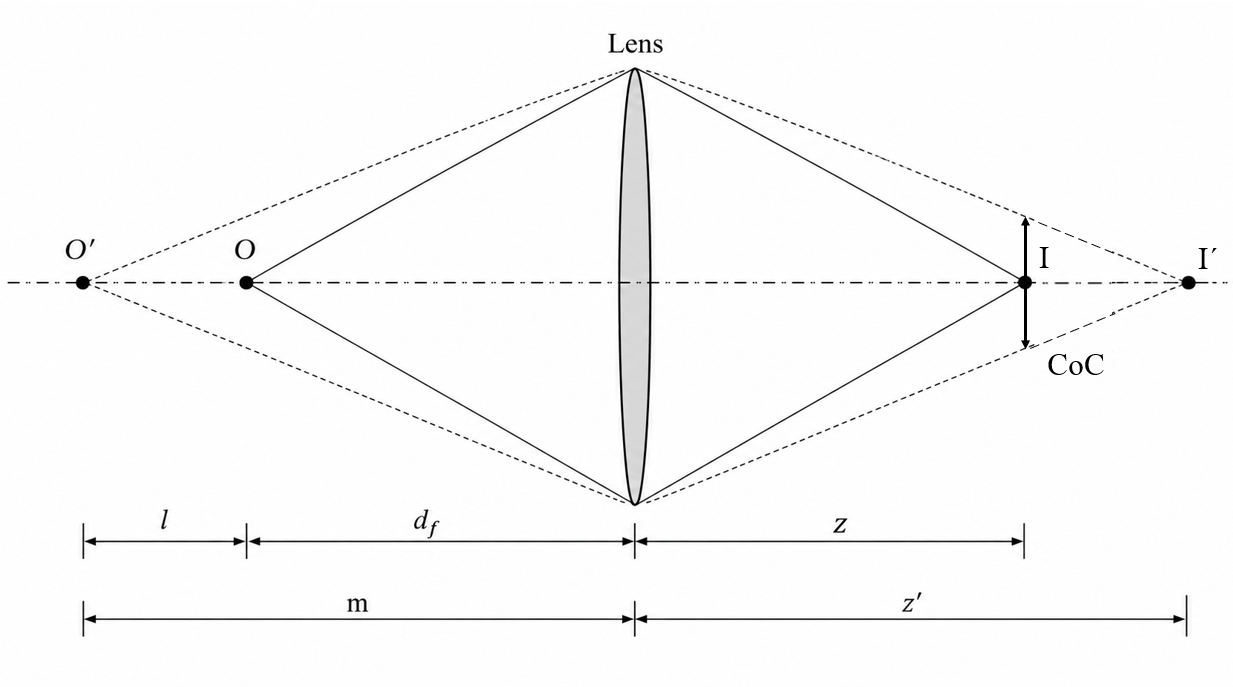
\includegraphics[width=0.8\textwidth]{figures/CoC drawing.png}
    \caption{Geometry of an out of focus object used to derive the CoC}
    \label{fig: CoC geometry}
\end{figure}

Through the ideal lens equation, $Z$ and $Z'$ can be written in the following form:


\begin{align}
    \label{equation: Z and Zprime}
    &Z = \frac{fd_f}{d_f-f}   & Z' = \frac{fm}{m - f}
\end{align}

Using triangle similarity, the relationship below can be established:

\begin{equation}
    \label{equation: CoC triangle similarity}
    \frac{CoC}{Z' - Z} = \frac{D}{Z'}
\end{equation}

Substituting Eq. \ref{equation: Z and Zprime} in relationship \ref{equation: CoC triangle similarity} and doing the necessary simplification, an explicit equation for $CoC$ is obtained:

\begin{equation}
    \label{equation: CoC explicit}
    CoC = \frac{f^2l}{f_\#m(d_f-f)}
\end{equation}

Where $f_\# = \frac{f}{D}$ is the lens f-stop number.

\par In Chapter \ref{chapter: methodology}, the sign of $l$ was considered to change depending on its position relative to the in-focus plane. This way, if an object finds itself behind the in-focus plane, Eq. \ref{equation: CoC explicit} will result in a negative $CoC$, while if the object is in front, it will be positive. Since the circle of confusion is a length, its absolute value can be considered in these cases.

\par Equation \ref{equation: CoC explicit} can also be modified by substituting it with Eq. \ref{equation: M and S definitions}, which define the magnification $Mag$ and sensitivity $S$

\begin{align}
        \label{equation: M and S definitions}
        &Mag = \frac{f}{d_f-f} & S = lMag
\end{align}

Resulting in:

\begin{align}
    \label{equation: CoC in M and S}
    & CoC = \frac{flMag}{f_\#m} & CoC = \frac{fS}{f_\#m}
\end{align}

The CoC is also in the core of another important parameter in optics called depth of field (DoF) \cite{Greenleaf1950}. The depth of field is the region around the in-focus plane where the $CoC$ is below a threshold deemed acceptable. This way, the depth of field can be interpreted as the thickness of the in-focus plane, where the image of all the objects inside this region is considered sharp enough. By definition, DoF can be calculated by subtracting the object distances $m_+$ and $m_-$ that produces the same $CoC$ when in front of the in-focus plane and behind it, respectively.

\chapter{Optics of a Blurred Object}
\label{Appendix: Blurred Object}

When an imaged object is blurred, its features do not converge to a single distinct point but are instead smeared around an area called circle of confusion. Figure \ref{fig: Blurred object geometry} shows an object of height $H'$ and how light travels from the highest point of the object to interact with the convergent lens in the sketch. The image also shows an object in focus with height $H$ and its image height $h$. Notice how the light rays from the in-focus object make a triangle with its image, it's this geometry that allows for the derivation of relationship between distances $d_f, f $ and $Z$ called thin lens equation, described in equation \ref{equation: Thin Lens equation}. For an out-of-focus object, the relationship between object distance $m$, image distance $Z$ and $f$ is no longer described through the thin lens equation as the geometry of the system has changed. Nevertheless, It is possible to use this new geometry to define new concepts, such as the blurred object magnification $M_{obj}$, which corresponds to the ratio between the size of the out-of-focus object and the image of the in-focus object that shares the light ray that crosses the middle of the lens with the out-of-focus object.

\begin{figure}[htbp]
    \centering
    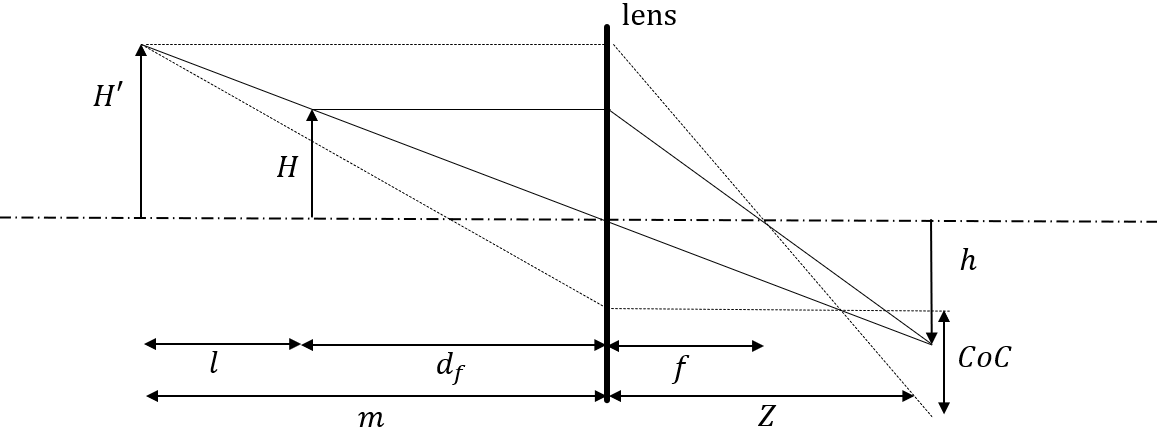
\includegraphics[width=0.8\textwidth]{figures/Blurred Object geometry.png}
    \caption{Geometry of an out of focus object}
    \label{fig: Blurred object geometry}
\end{figure}


\begin{equation}
    \label{equation: Mobj definition}
    M_{obj} = \frac{h}{H'} = \frac{Z}{m}
\end{equation}

This magnification can also be written in terms of the focal length and the in-focus magnification:

\begin{equation}
    \label{equation: Mobj in f and M}
    M_{obj} = \frac{f(1+M)}{m}
\end{equation}

Equivalently to how $M$ can be used to transfer a length from the image plane to the object plane and vice-versa by dividing or multiplying it by $M$, respectively. The same can be done with $M_{obj}$. This way, it is possible to transfer the $CoC$ from the image plane to the blurred object plane. In this same way, $L_{FoV_{obj}}$ was derived in equation \ref{equation: LFoVobj BOS}.

\begin{equation}
    \label{equation: CoCobj transfer}
    CoC_{obj} = \frac{CoC}{M_{obj}}
\end{equation}

By combining equations \ref{equation: CoC in M and S}, \ref{equation: Mobj in f and M} and \ref{equation: CoCobj transfer}, it is possible to obtain:

\begin{equation}
    \label{equation: CoCobj compact}
    CoC_{obj} = \frac{lM}{f_\#(1+M)}
\end{equation}

and rearranging equations \ref{equation: CoCobj transfer} and \ref{equation: Mobj definition}, following the geometry of Figure \ref{fig: Geometry BOS}:

\begin{equation}
    \label{equation: CoCobj expanded}
    CoC_{obj} = \frac{CoC}{M} \frac{m}{d_f} = \frac{CoC}{M} \left( 1 - \frac{l}{m+l}\right)
\end{equation}

Given the spatial resolution $\delta_t$ derived by Gojani \& Obayashi, described by equation 10 on their article \cite{Gojani&Obayashi}.

\begin{equation}
\label{equation: Gojani SR formulation}
    \delta_t = \frac{lM}{f_\#(1+M)} + \frac{\Delta_t}{M} \left( 1 - \frac{l}{m+l}\right)
\end{equation}

If $\Delta_t$ corresponds to the $CoC$ as it is mentioned in Gojani's paper, his blurred circle becomes $\delta_t = 2 \cdot CoC_{obj}$ through equations \ref{equation: CoCobj compact} and \ref{equation: CoCobj expanded}. It is thus proven that Gojani’s formulation predicts a blur circle twice the size of the one established experimentally by Schwarz and Braukmann \cite{Gojani&Obayashi, Schwarz&Braukmann}.

\chapter{Extended Design Space Surface Maps}
\label{Appendix: Supplementary Surface Maps}

\par This appendix collects the surface maps that were computed by the design space exploration of Chapter \ref{chapter: methodology} but were not reproduced in the main text. They are provided for completeness and to support the validation of the design strategy during the first experimental campaign.

\section{Pixel density and in-focus field of view}
\label{section: Appendix pixel density}

\par Figure \ref{fig: Px pitch and LFOV surfmap SBOS} displays the pixel density $\rho_{px}$ and the field of view of the in-focus plane $L_{FoV}$ for the negative defocus setup of Section \ref{subsection: Surface Maps for SBOS}. Both quantities depend only on the optical magnification, through Equation \ref{equation: Px density} and $L_{FoV} = L_{sens}/M_{ag}$, so they present the same trends as $M_{ag}$ in Figure \ref{fig: M,m and df design surfmap SBOS}. The pixel density increases with $l$ and decreases with $f$, while $L_{FoV}$ shows the inverse behavior. The in-focus plane is where the calibration plate is positioned, therefore these maps can be directly compared to the measured values during the experimental campaign.

\begin{figure}[htbp]
    \centering
    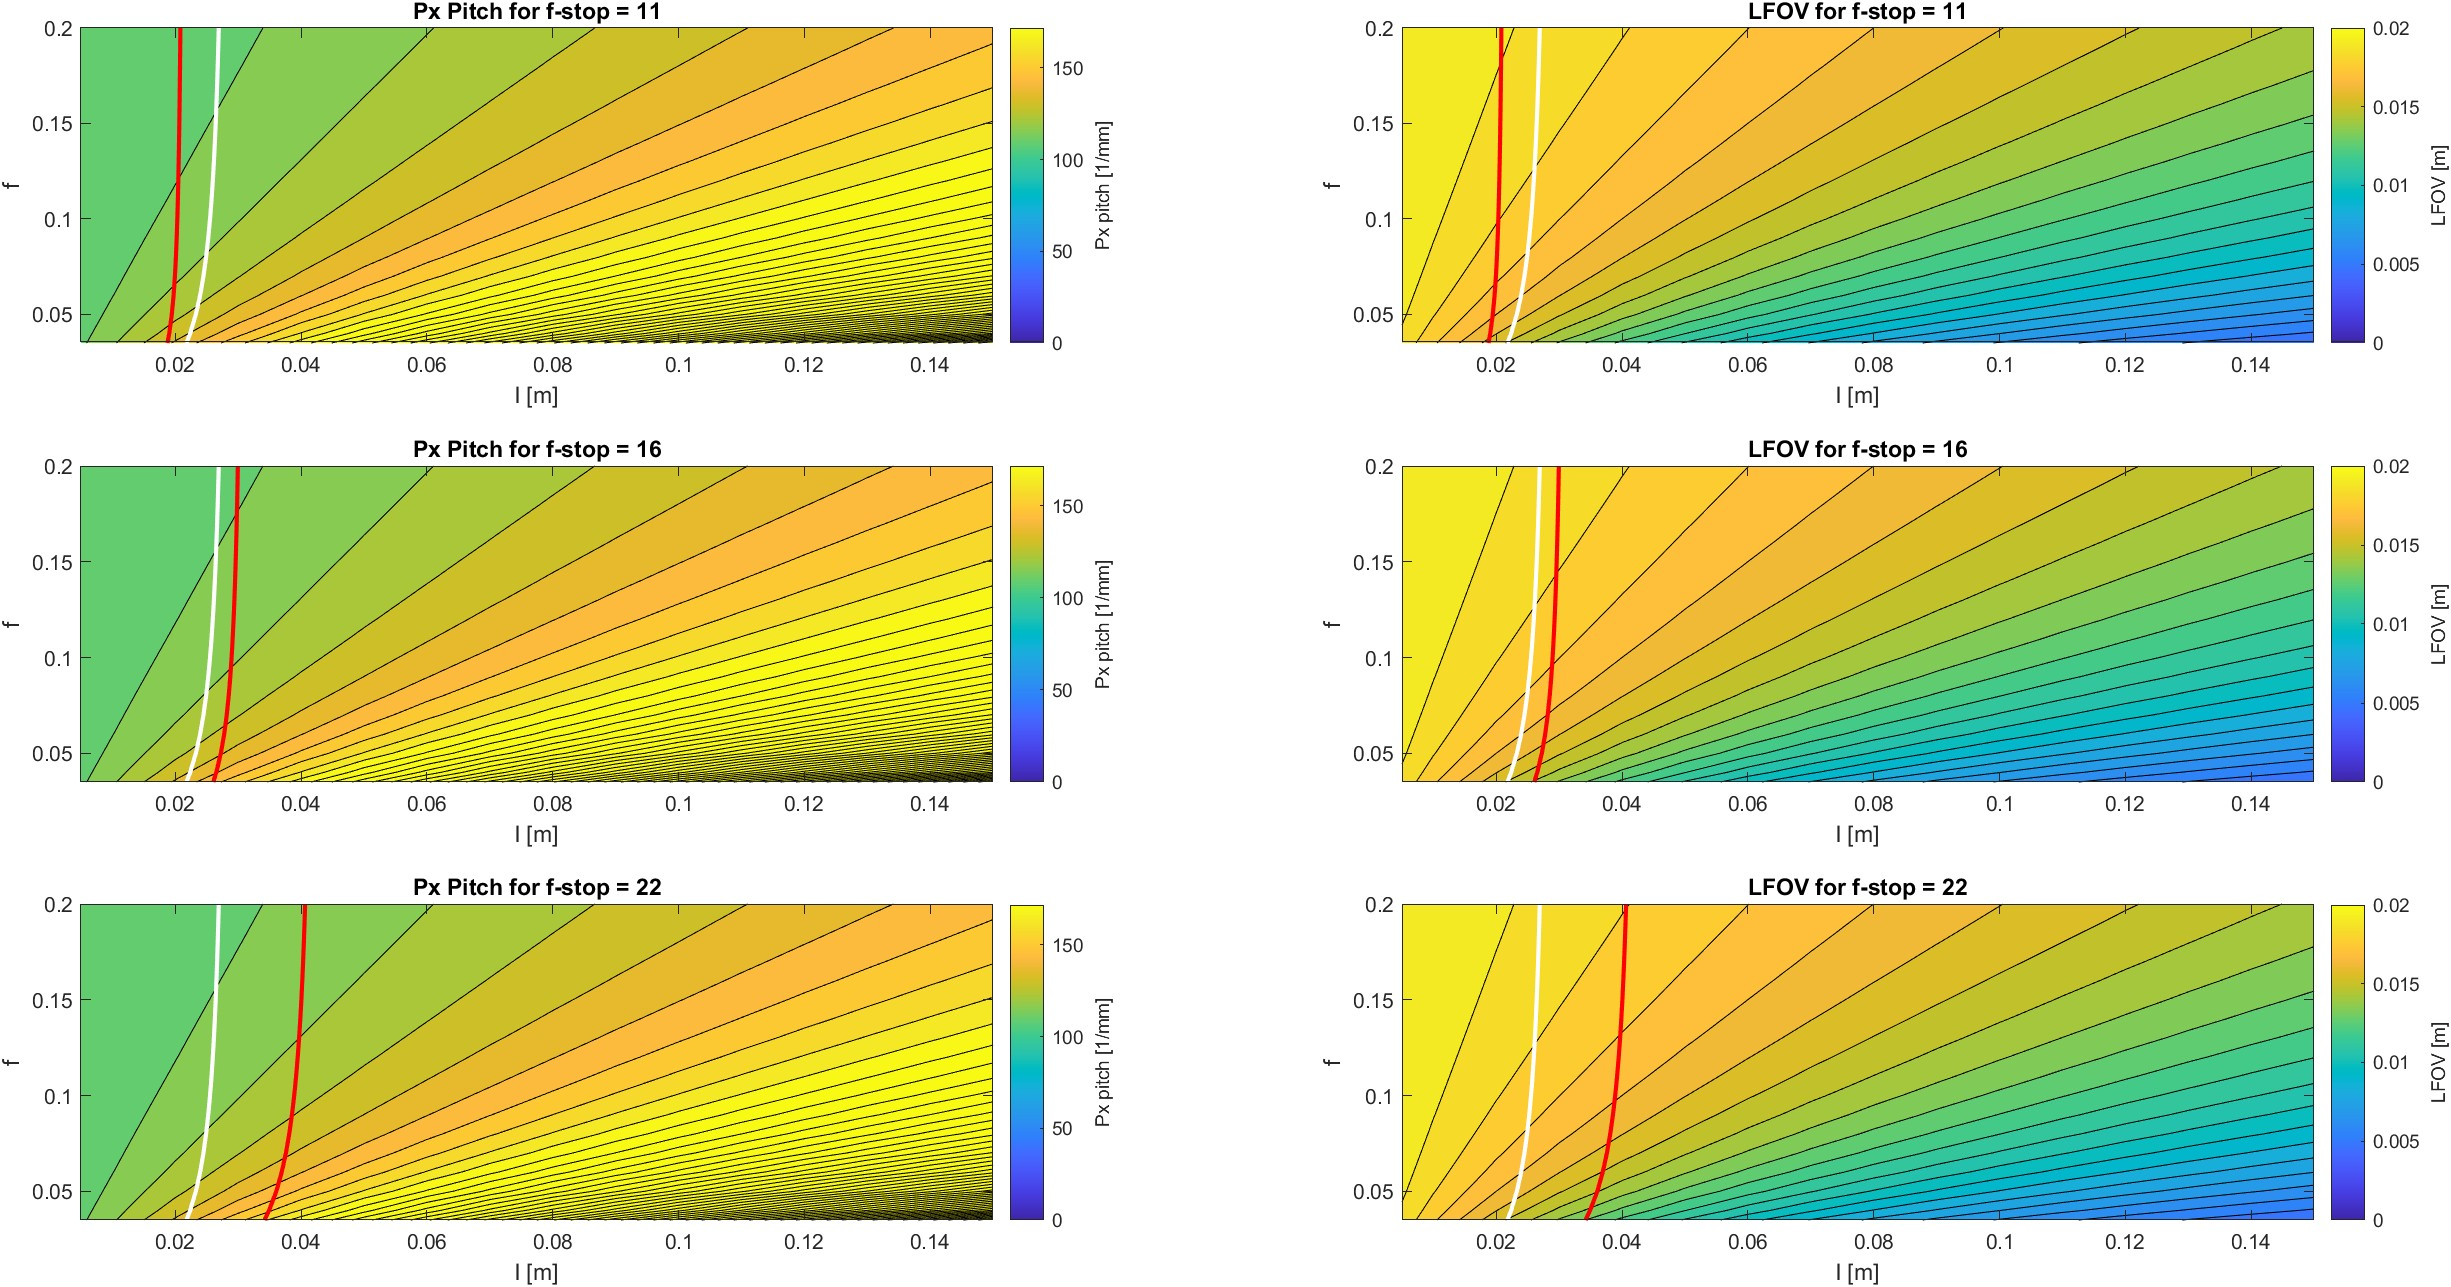
\includegraphics[width=1\textwidth]{figures/Px pitch and LFOV SBOS surf map.jpg}
    \caption{Surface maps of $\rho_{px}$ and $L_{FoV}$ for $f_\# \in $ [11,16,22],  $f \in $ (0.035,0.200), $l \in$ (0.005,0.15) and $L_{FoV_{obj}}=$ 2cm of a negative defocus setup, with the red isoline representing the points where $s_{min}$ =0.0004 m and the white line showing $S=0.02$.}
    \label{fig: Px pitch and LFOV surfmap SBOS}
\end{figure}

\section{Speckle size for positive defocus}
\label{section: Appendix speckle size BOS}

\par Figure \ref{fig: Delta s surfmap BOS} displays the speckle size of the positive defocus setup of Section \ref{subsection: Surface maps for BOS}. As in the negative defocus case, $\Delta s$ follows the trends of $M_{ag}$ through Equation \ref{equation: Rayleigh Limit}. It decreases with $l$ and increases with $f$, which is the inverse of the trend in Figure \ref{fig: Delta s design surfmap SBOS}. The smaller magnification of the positive defocus setup results in smaller speckles for the same $f_\#$, and both configurations converge to the same speckle size as $l$ approaches zero.

\begin{figure}[htbp]
    \centering
    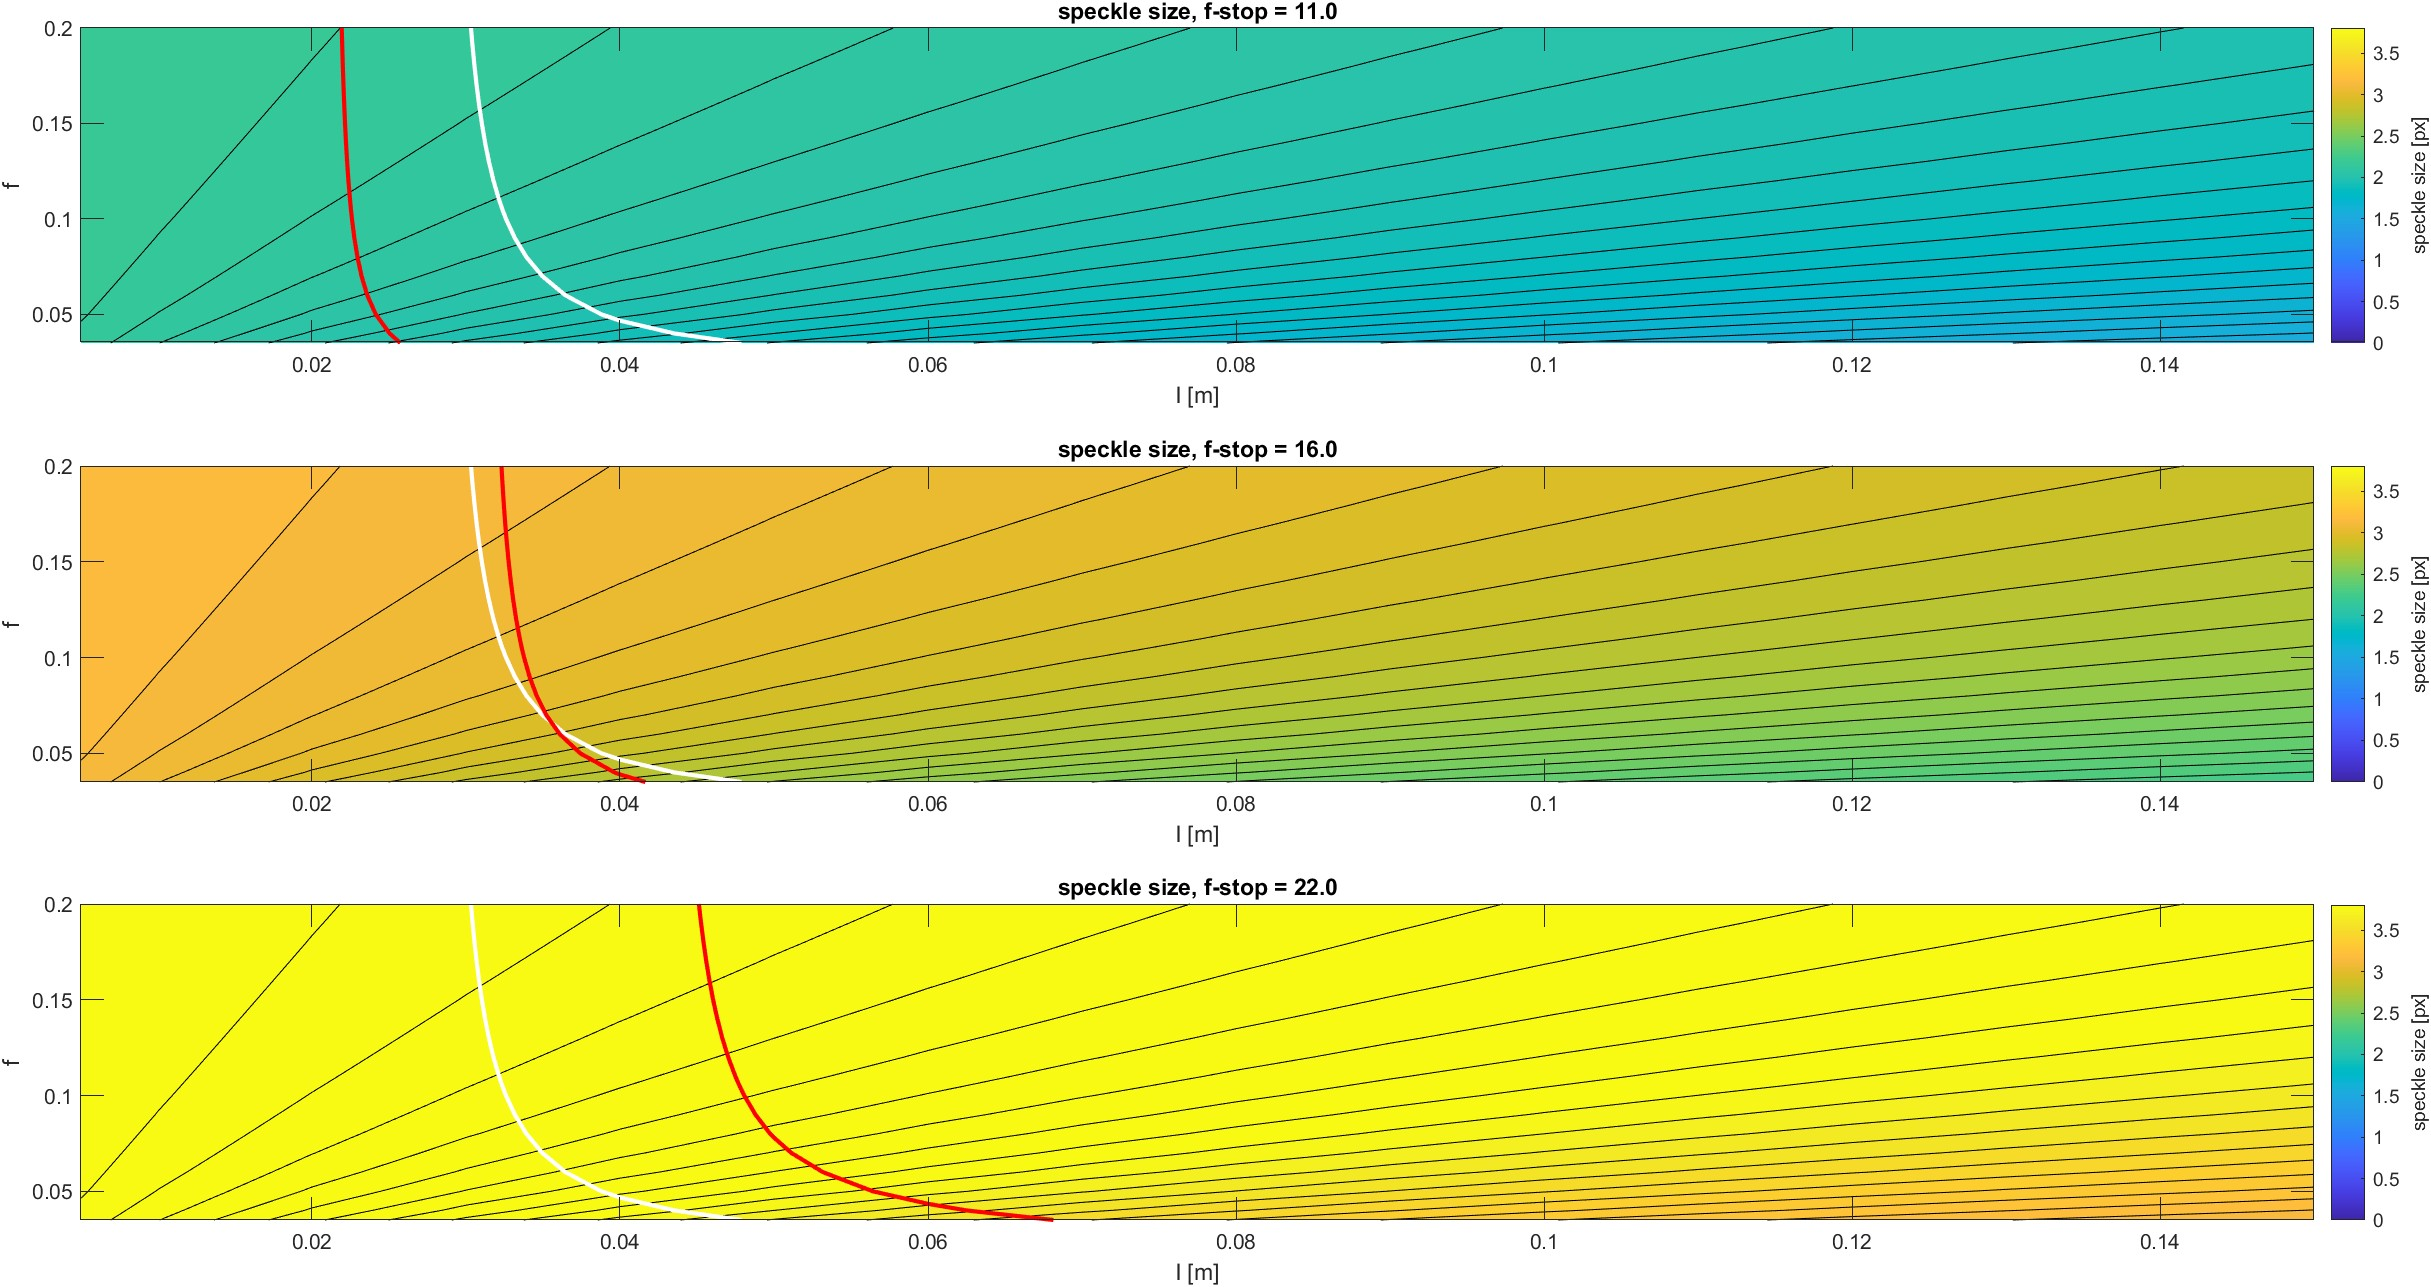
\includegraphics[width=1\textwidth]{figures/Speckle size surf map BOS.jpg}
    \caption{Surface maps of $\Delta s$ for $f_\# \in $ [11,16,22],  $f \in $ (0.035,0.200), $l \in$ (0.005,0.15) and $L_{FoV_{obj}}=$ 2cm of a positive defocus setup, with the red isoline representing the points where $s_{min}$ =0.0004 m and the white line showing $S=0.02$.}
    \label{fig: Delta s surfmap BOS}
\end{figure}

\section{Surface maps for a 7 cm field of view}
\label{section: Appendix 7cm FoV}

\par Figures \ref{fig: M,m,df surfmap SBOS 70mm} and \ref{fig: M,m,df surfmap BOS 70mm} display $M_{ag}$, $m$ and $d_f$ of the negative and positive defocus setups for $L_{FoV_{obj}} = 7$ cm, while Figure \ref{fig: Delta s surfmap 70mm} displays the respective speckle sizes. The trends are the same as the ones found for $L_{FoV_{obj}} = 2$ cm in Section \ref{section: Design Strategy}. The larger field of view, however, requires smaller magnifications and larger distances $m$ and $d_f$, which explains the smaller $S$ and $s_{min}$ discussed in Section \ref{subsection: Effects of FoV}. The smaller magnification also reduces the speckle size through Equation \ref{equation: Rayleigh Limit}.

\begin{figure}[htbp]
    \centering
    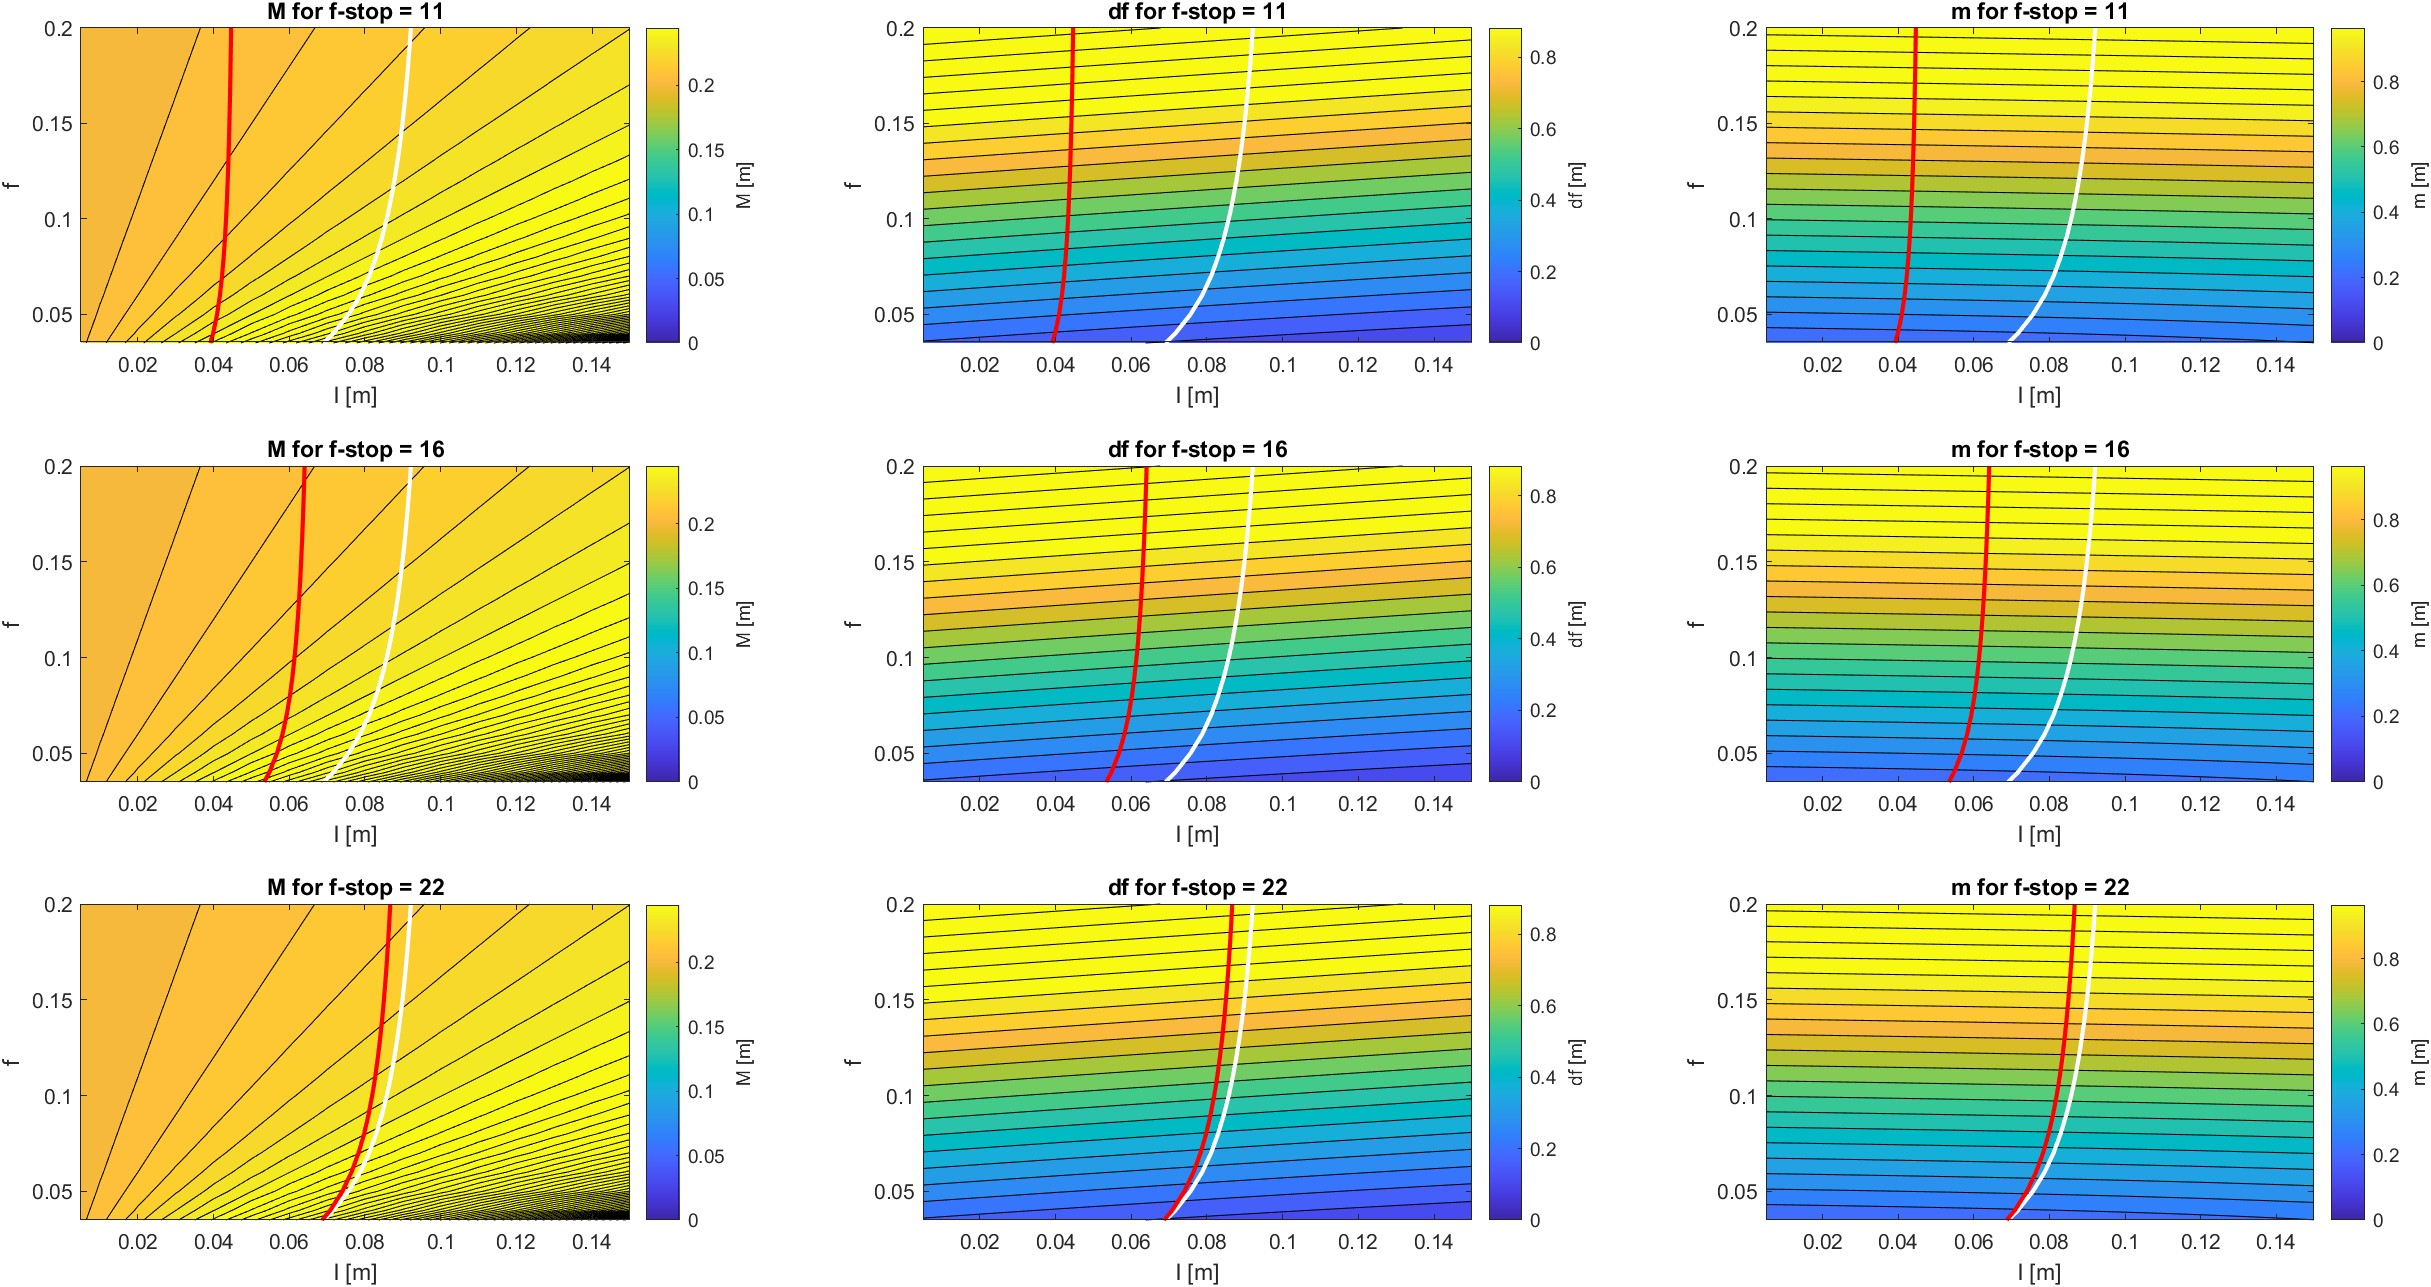
\includegraphics[width=1\textwidth]{figures/M,m,df surfmaps SBOS 70mm.jpg}
    \caption{Surface maps of $M_{ag}$, $m$ and $d_f$ for $f_\# \in $ [11,16,22],  $f \in $ (0.035,0.200), $l \in$ (0.005,0.15) and $L_{FoV_{obj}}=$ 7cm of a negative defocus setup, with the red isoline representing the points where $s_{min}$ =0.00035 m and the white line showing $S=0.02$.}
    \label{fig: M,m,df surfmap SBOS 70mm}
\end{figure}

\begin{figure}[htbp]
    \centering
    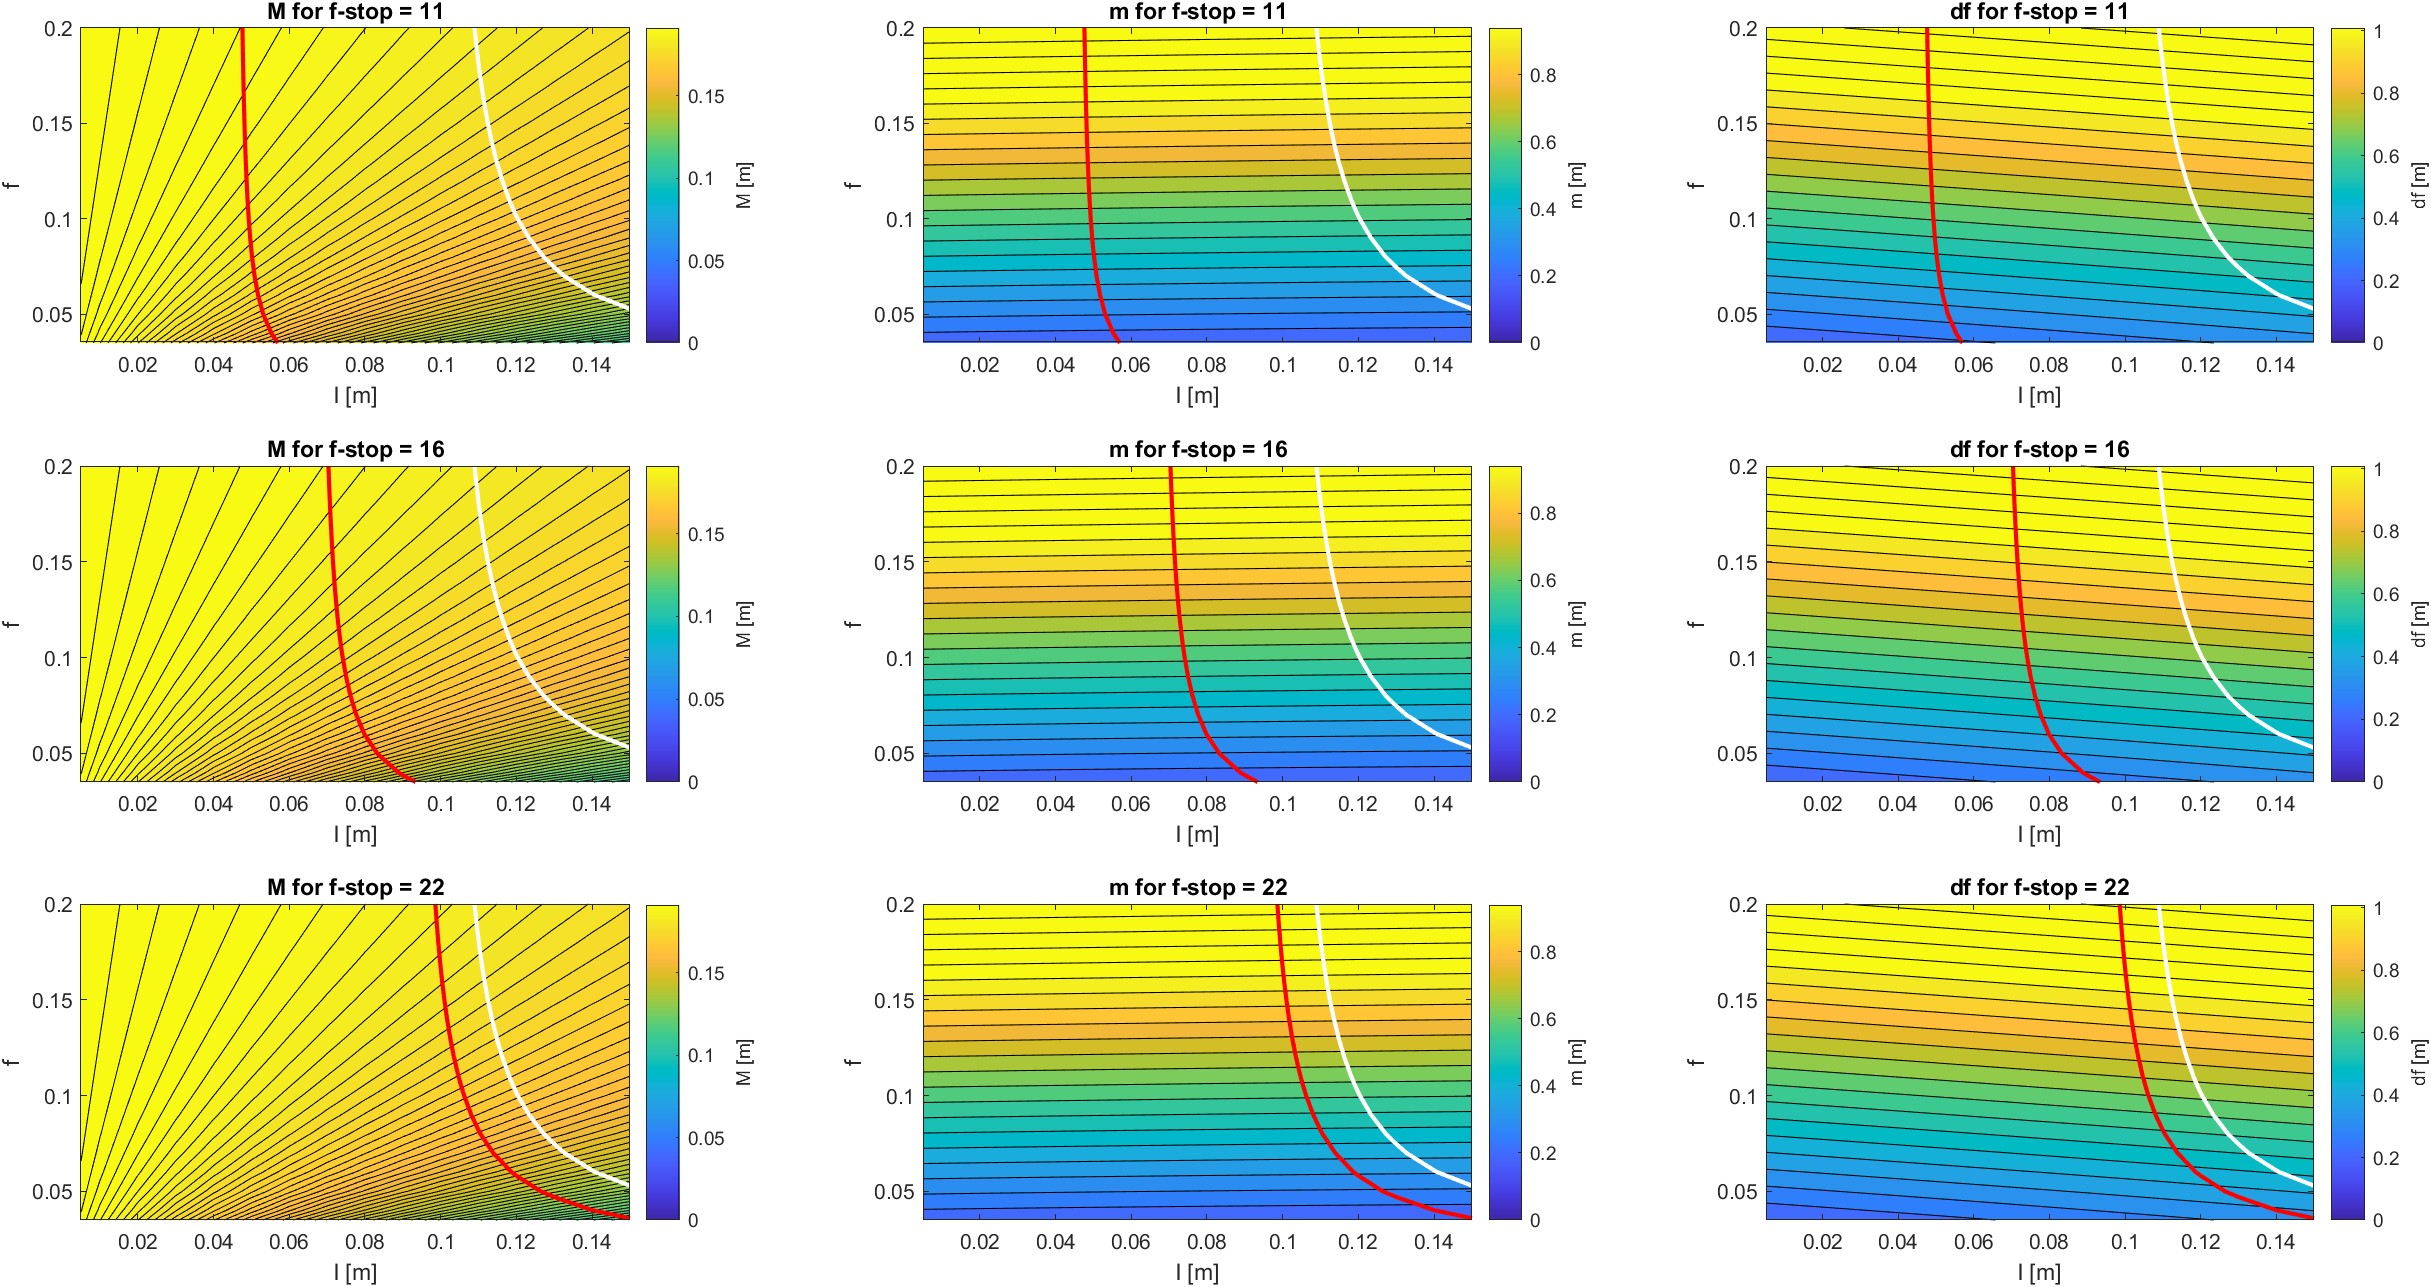
\includegraphics[width=1\textwidth]{figures/M,m,df surfmaps BOS 70mm.jpg}
    \caption{Surface maps of $M_{ag}$, $m$ and $d_f$ for $f_\# \in $ [11,16,22],  $f \in $ (0.035,0.200), $l \in$ (0.005,0.15) and $L_{FoV_{obj}}=$ 7cm of a positive defocus setup, with the red isoline representing the points where $s_{min}$ =0.00035 m and the white line showing $S=0.02$.}
    \label{fig: M,m,df surfmap BOS 70mm}
\end{figure}

\begin{figure}[htbp]
  \centering
  \begin{subfigure}{0.9\textwidth}
    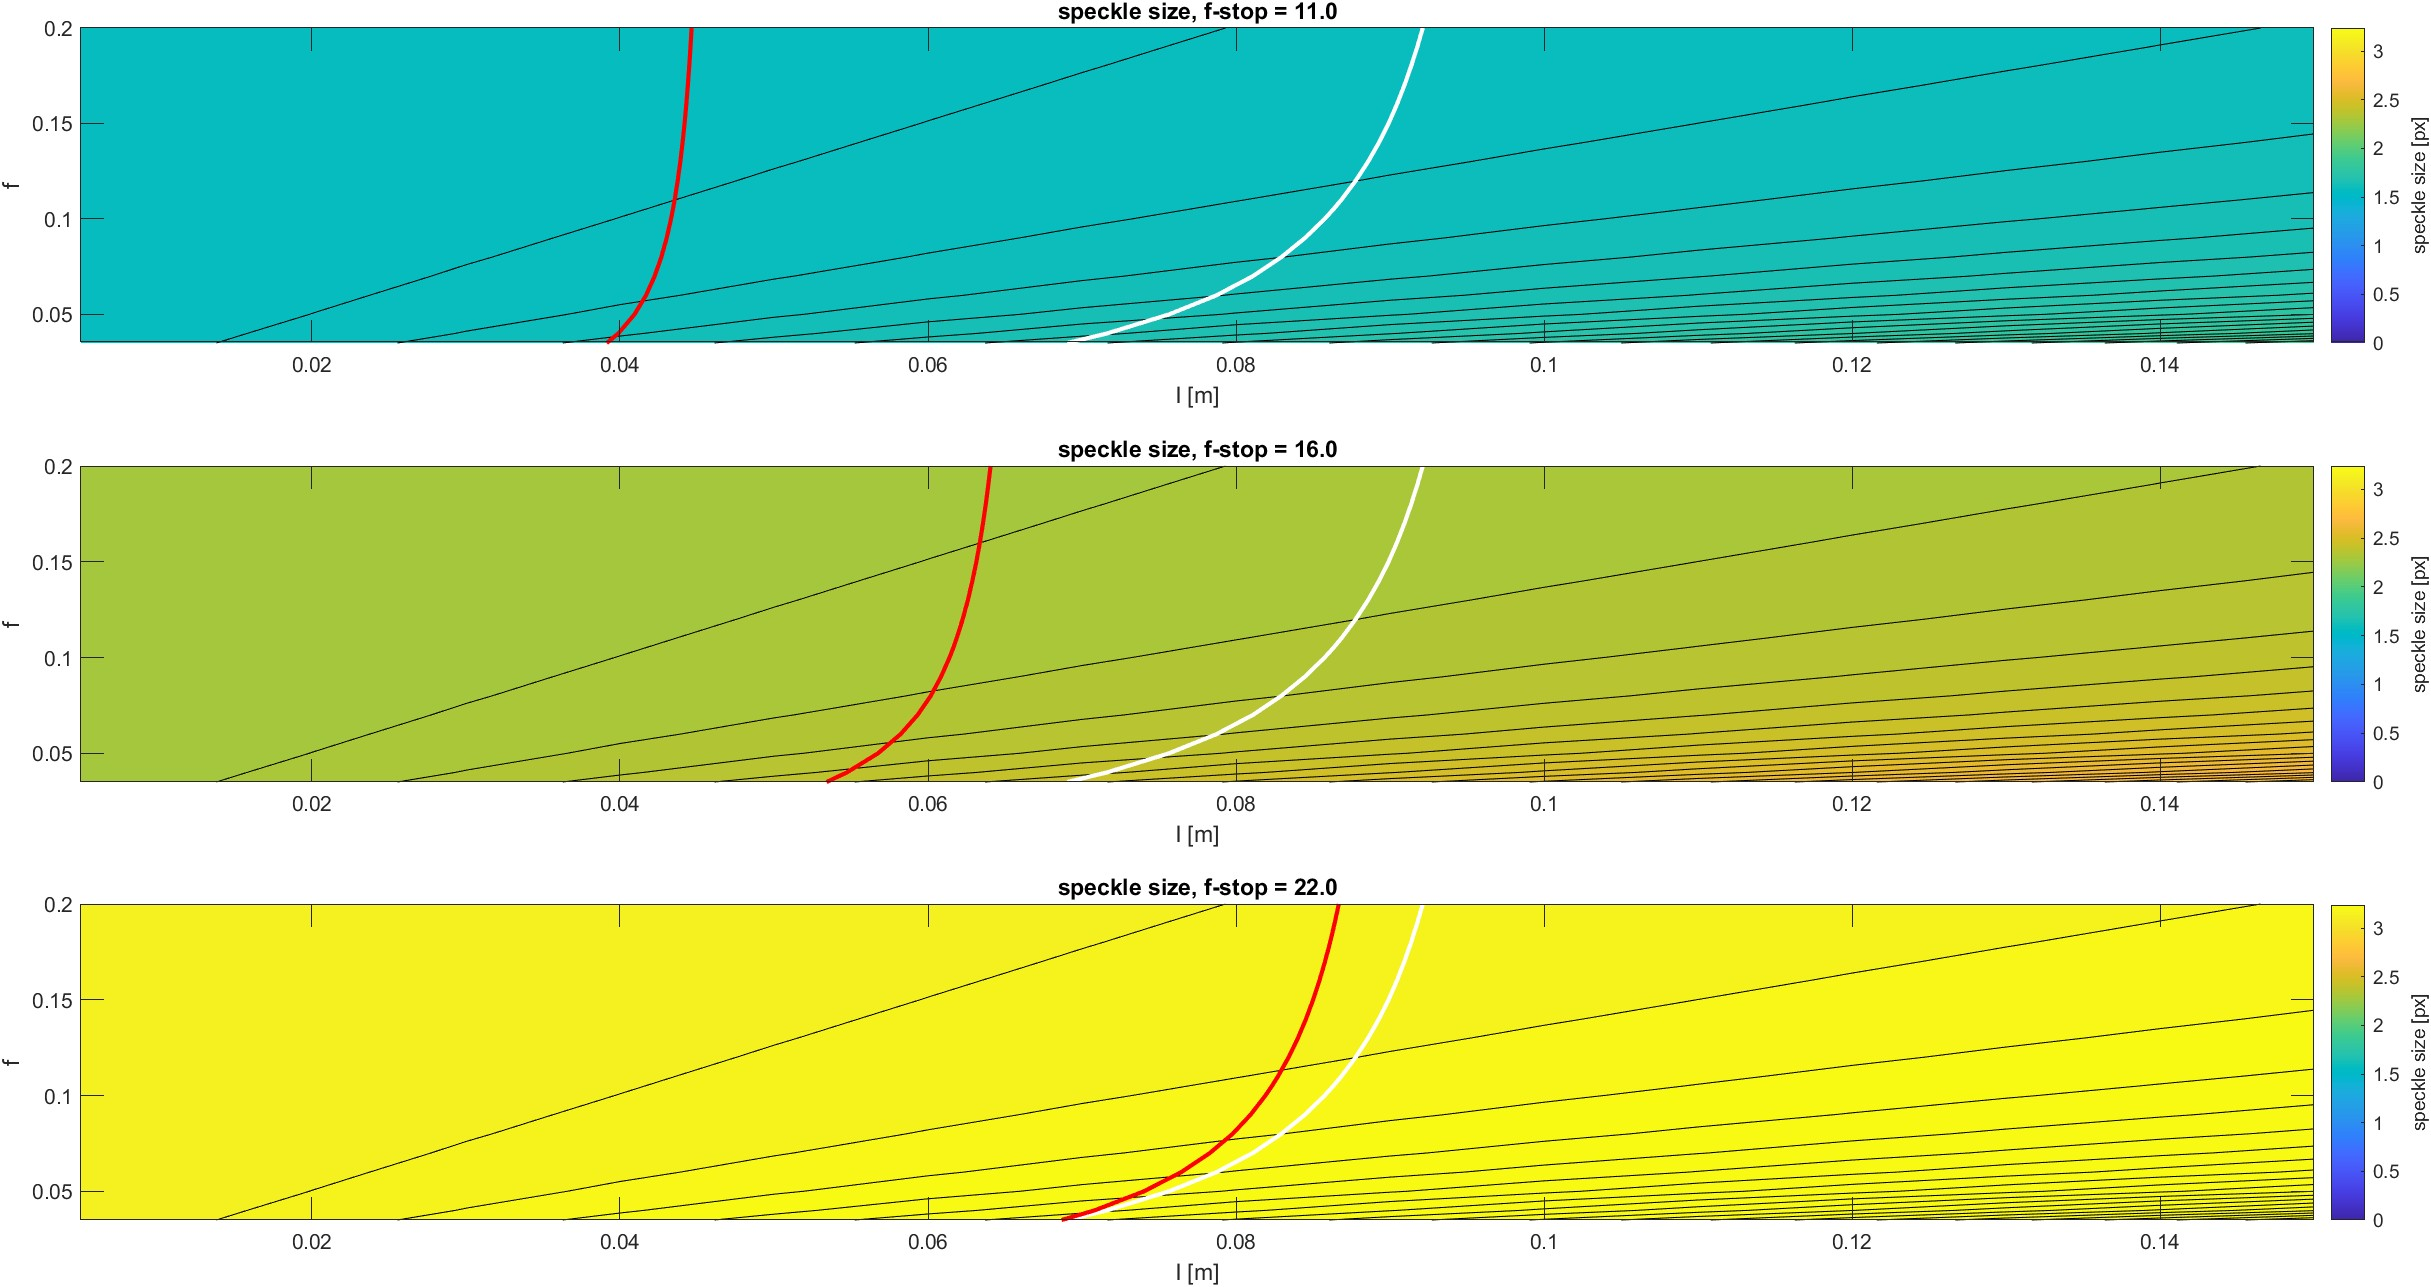
\includegraphics[width=\textwidth]{figures/Speckle size surf map SBOS 70mm.jpg}
    \caption{}
    \label{fig: Delta s surfmap SBOS 70mm}
  \end{subfigure}

  \begin{subfigure}{0.9\textwidth}
    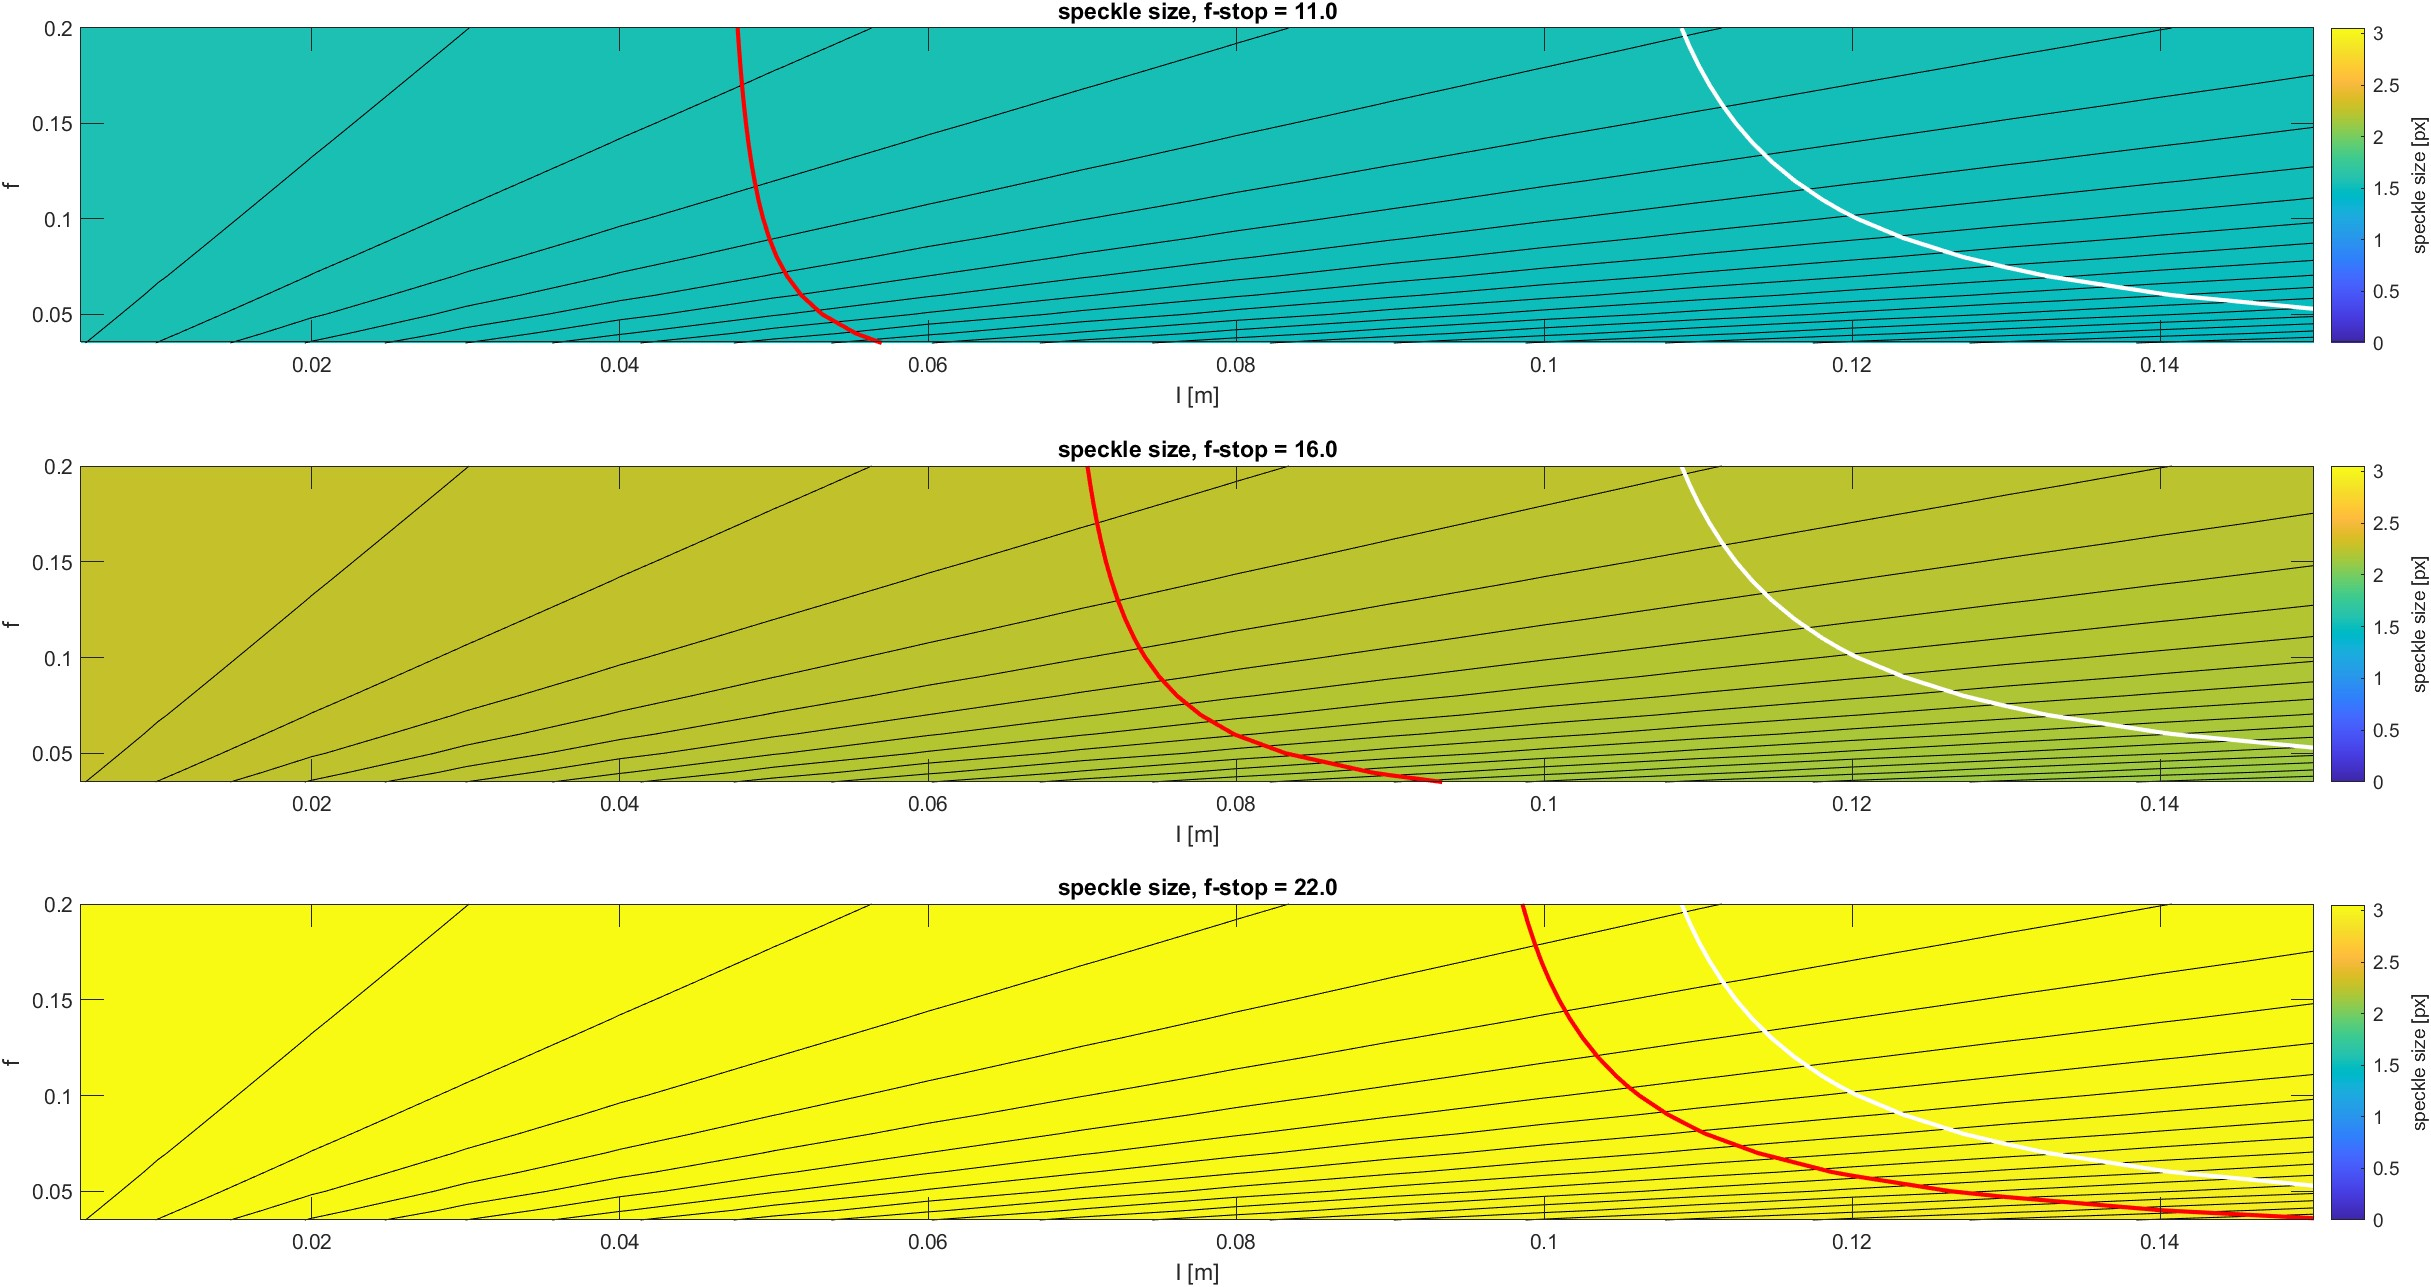
\includegraphics[width=\textwidth]{figures/Speckle size surf map BOS 70mm.jpg}
    \caption{}
    \label{fig: Delta s surfmap BOS 70mm}
  \end{subfigure}
  \caption{Surface maps of $\Delta s$ for $f_\# \in $ [11,16,22],  $f \in $ (0.035,0.200), $l \in$ (0.005,0.15) and $L_{FoV_{obj}}=$ 7cm of a negative defocus setup (a) and a positive defocus setup (b), with the red isoline representing the points where $s_{min}$ =0.00035 m and the white line showing $S=0.02$.}
  \label{fig: Delta s surfmap 70mm}
\end{figure}


\end{document}
